%% Generated by Sphinx.
\def\sphinxdocclass{report}
\documentclass[letterpaper,11pt,catalan]{sphinxmanual}
\ifdefined\pdfpxdimen
   \let\sphinxpxdimen\pdfpxdimen\else\newdimen\sphinxpxdimen
\fi \sphinxpxdimen=.75bp\relax

\usepackage[utf8]{inputenc}
\ifdefined\DeclareUnicodeCharacter
 \ifdefined\DeclareUnicodeCharacterAsOptional\else
  \DeclareUnicodeCharacter{00A0}{\nobreakspace}
\fi\fi
\usepackage{cmap}
\usepackage[T1]{fontenc}
\usepackage{amsmath,amssymb,amstext}
\usepackage{babel}
\usepackage{times}
\usepackage[Sonny]{fncychap}
\usepackage{longtable}
\usepackage{sphinx}

\usepackage{geometry}
\usepackage{multirow}
\usepackage{eqparbox}

% Include hyperref last.
\usepackage{hyperref}
% Fix anchor placement for figures with captions.
\usepackage{hypcap}% it must be loaded after hyperref.
% Set up styles of URL: it should be placed after hyperref.
\urlstyle{same}
\addto\captionscatalan{\renewcommand{\contentsname}{Continguts:}}

\addto\captionscatalan{\renewcommand{\figurename}{Fig.}}
\addto\captionscatalan{\renewcommand{\tablename}{Table}}
\addto\captionscatalan{\renewcommand{\literalblockname}{Listing}}

\addto\extrascatalan{\def\pageautorefname{page}}

\setcounter{tocdepth}{1}



\title{Software d'integració d'escaneig i gestió documental}
\date{jul. 03, 2017}
\release{Memòria}
\author{Francesc Puig Plana}
\newcommand{\sphinxlogo}{}
\renewcommand{\releasename}{Versió}
\makeindex

\begin{document}

\maketitle
\sphinxtableofcontents
\phantomsection\label{\detokenize{index::doc}}



\chapter{Introducció, motivacions, propòsit i objectius del projecte}
\label{\detokenize{index:software-dintegracio-global-descaneig-i-gestio-documental}}\label{\detokenize{index:introduccio-motivacions-proposit-i-objectius-del-projecte}}

\section{Introducció}
\label{\detokenize{index:introduccio}}
Cada cop és més necessari la utilització de documents en format digital, amb tot
el que això comporta. Digitalitzar, emmagatzemar, distribuir, ordenar, consultar i modificar un gran volum
de documents pot arribar a ser una tasca tediosa.

Això fa que moltes empreses es proposin buscar una solució per automatitzar aquests processos.
El primer pas és comptar amb una base informàtica, i després plantejar com organitzar aquests documents.
Existeixen diverses solucions software, i una bona base és la metodologia que
proposen els gestors documentals. Un gestor documental intenta integrar totes aquestes
característiques i fer molt més fàcil els processos que respecten al tractament dels fitxers,
automatitzant les tasques típiques d'aquests, tant l'obtenció del document en format digital,
com l'edició i la postclassificació.
Automatitzant tasques es pot arribar a aconseguir un procés molt més àgil. En països hispans s'utilitza el terme
gestió documental, tot i que comptant amb les característiques actuals de les empreses és més correcte
utilitzar el terme anglosaxó \sphinxstyleemphasis{Enterprise Content Manager -ECM-}, atès que les empreses utilitzen un
ampli ventall de tipus d'arxius digitals.

De la necessitat de contribuir amb el medi ambient i el maldecap que suposa l'emmagatzemament en format paper
dels documents, ha sorgit la metodologia \sphinxstylestrong{paperless}, que concretament proposa la unificació de dades digitalitzades
i l'estalvi de documents en format paper. Ja no només es parla d'estalvi de paper, sinó de classificació i espai,
que pot arribar a ser un verdader maldecap. Però amb tal volum de dades digitalitzades cal remarcar
que l'organització hi juga un paper clau, i és aquí on entra el rol de la gestió documental. Si
es pensa i s'analitza la quantitat de documents que genera tan sols una petita/mitjana empresa
en el seu dia a dia, de seguida sorgeix la necessitat d'una bona base per gestionar-ho, i no tan sols per l'organització,
sinó per l'obtenció, visualització... d'aquests documents. Això no vol dir que no s'estigui preparat,
però altres metodologies com aquesta fan clar l'estalvi de temps, recursos... i això òbviament es pot
traduir en guanys econòmics. Parlant d'estar preparats, qualsevol pot tenir el seu sistema, però
subjectivament sóc partidari d'indagar amb la nova tecnologia, que no només ha de servir per tenir
una vida quotidiana plena d'avantatges i/o facilitats. Al primer graó de la tecnologia vanguardista
hi ha d'haver aquella que ajudi al progrés de les empreses.

Anàlogament un sistema de gestió documental permet augmentar l'eficiència de treball
automatitzant i agilitzant tasques molt comunes del dia a dia en la gran majoria d'empreses, en
el que el tractament de documents es refereix.
Observant l'esmentat anteriorment, són moltes les funcionalitats que pot tenir un software d'aquestes
característiques, l'aplicació pot integrar processos de reconeixement de fitxers, visualitzadors
per categoria, analitzadors de malware o documents erronis, processos post classificació...
Bàsicament ajuden a l'usuari a gestionar aquests processos, segons la necessitat de cadascú,
i afegeix intel·ligència per tal de classificar, comprovar... o el que sigui necessari amb aquesta
base de documents.

Per tal de donar una cara més familiar a un gestor documental, es pot definir en paraules trivials
com un \sphinxstyleemphasis{contenidor} de documents intel·ligent, que no només ajuda amb l'obtenció del fitxer (foto, vídeo, document
de text pla...), sinó que t'organitza en directoris, seccions... (el que es vulgui), aquests documents.
A més se li poden aplicar les característiques que es vulguin (edició de documents, filtratge antimalware,
màscares de documents...), i proporciona una base classificada de tots aquests arxius. A tall
d'exemple, es podria veure com una biblioteca ben organitzada de documents amb
un empleat que no tan sols organitza i posa a disposició de qui ho necessiti certs fitxers, sinó que
ajuda i automatitza la mateixa obtenció dels esmentats.

Per posar color a la temàtica, ara suposem una tasca que realitzaria un empleat d'una empresa x
per digitalitzar i adjuntar una factura d'un cert client, sense cap base gestió documental.
Pensem que el client es persona a la suposada empresa, juntament amb més clients que esperen
impacients el seu torn. L'empleat escaneja el document, l'aplicació demana on desar-lo,
el desa en qualsevol directori del pc físic, busca el programa, l'obre, busca el client, es
dirigeix a l'apartat de factures, busca la referència, selecciona \sphinxstyleemphasis{adjuntar factura},
busca en el directori la factura que acaba de digitalitzar, la selecciona i l'adjunta al programa.
Ara suposem que aquest empleat té un software
d'integració i gestió documental: Obre el programa, cerca el client i digitalitza el document.
El mateix software ha aconseguit digitalitzar i classificar la factura respectiva al client
seleccionat, no calen més passos i ja pot atendre al següent client. Vegem-ho en forma de diagrama.

Cas 1


\includegraphics{graphviz-730df8cc302261870b3aa4a08e51901844830eb1.pdf}

Cas 2

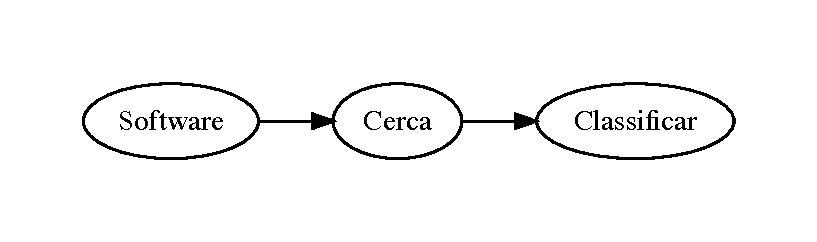
\includegraphics{graphviz-c379de371ff5e28e2a5a8c8e959c158df1237304.pdf}

El procés de digitalització de documents és fonamental per representar digitalment el mapa de
bits d'un document en format paper, mitjançant aquest procés s'emmagatzema en una base de dades a la
qual tindran accés les persones autoritzades de l'arxiu o informació capturada. Al final el procés
sempre és el mateix i es basa en convertir un origen no digital a una representació digital. El gran
embroll de tot això és l'organització, si en format paper és complicat, en format digital també
pot suposar un problema, ja que no només és necessari un espai en disc sinó que calen mètodes
d'organització i accés.

La necessitat d'aquest tipus de software, la proposta feta pels mentors i les ganes
d'indagar en una metodologia desconeguda han estat claus per l'elecció d'aquest projecte.
Tot discutint mentalment en què dedicaria les hores en els següents mesos, en els que em
tocava fer el projecte, tenia clar que volia fer quelcom que m'apassionés, que m'aportés coneixement
i motivació. Tenia diverses idees mig difuminades quan em varen donar l'oportunitat de realitzar
aquest projecte, no vaig dubtar. Al veure les cares dels qui m'ho proposaven vaig veure que
era un projecte necessari, i interessant. Mai no he cregut en els projectes de fons d'armari,
que acaben oblidats sota un munt de folis.


\section{Motivacions i propòsit}
\label{\detokenize{index:motivacions-i-proposit}}
Com a opinió personal em reservo el dret de dir que qualsevol projecte o treball a realitzar és
molt important que hom se'l faci seu, que el senti tangible i que sobretot cregui en la importància d'aquest.
D'aquesta manera es torna motivador realitzar-lo, i sempre es rep un feedback positiu quan és així.
Clar està que treballant a gust fa que tot es torni més de cara. D'aquesta manera les coses surten
millor, el projecte avança fluidament i a més a canvi n'obtens una satisfacció, no només per estar o
haver realitzat un projecte o treball sinó d'estar-ne aprofitant la avinentesa per gaudir i créixer
en l'àmbit de treball en què es realitza. Grans empreses conegudes com Google utilitzen mètodes
de treball motivadors per als seus empleats al·legant que un treballador content realitza un volum més
ampli de feina i de més qualitat. Els beneficis de treballar així no tan sols es veuen reflectits
en el producte final sinó que ajuden a fer passional allò que s'està fent en cada moment del qual dura
el procés. Per tant, invertir una mica més de temps en buscar un bon tema, una bona proposta, un bon
entorn de treball, i la motivació, són claus per aconseguir tot el relatat. A més, com a extra està bé
aprofitar l'ocasió per escollir metodologies i estils de treball que sempre havies volgut provar,
donant més força així a la motivació del treball.

Anecdòticament el dia que vaig tenir clar el tema, vaig tenir una conversa on sense jo explicar
sobre el que volia fer el TFG, em van expressar el necessari que seria un software d'aquestes
característiques, comentant un tema relacionat amb l'advocacia, va ser llavors quan em va
fer il·lusió comentar que precisament el treball que començava tractava del mateix.

Per situar el lector en el marc d'aquest treball, aquest TFG es realitza a l'empresa GISCE-TI, S.L.
Un client havia demanat un software d'integració d'escaneig i gestió documental. En capítols posteriors
es detallaran més a fons les característiques i el treball empresa - client, però és interessant
deixar clar que aquest projecte es desenvolupa a l'empresa per servir el producte al client
que l'ha sol·licitat. Per tant ja està \sphinxquotedblleft{}col·locat\sphinxquotedblright{} abans de presentar-lo, ja que es desenvoluparà
per al client.


\section{L'Empresa}
\label{\detokenize{index:l-empresa}}
El projecte es desenvolupa a l'empresa, i a fi de presentar la situació actual, es tracta breument
les característiques d'aquesta.
L'empresa on es realitza aquest TFG és GISCE-TI, S.L. una empresa Gironina especialitzada en
servir solucions software a les empreses del sector elèctric, tant distribuïdores com comercialitzadores.
A GISCE, hi treballa un equip de programadors per assolir i desenvolupar aquestes solucions
software. El producte estrella és un ERP integral que ajuda a satisfer les necessitats d'aquests
tipus d'empreses. També hi ha el departament d'Enginyeria que es dedica a inspeccions, auditories...

Aquest TFG tracta de desenvolupar una solució software sol·licitada per una empresa client, que es pugui
integrar també en el treball funcional i diari d'aquest ERP, i que més endavant hi hagi
la possibilitat de desplegar-ho a altres clients.

Els productes que serveix l'empresa, són Software lliure, i la filosofía de treball que
utilitzen és donar suport a les empreses que sol·liciten els productes, a nivell usuari o
a nivell informàtic. També ajuden a l'automatització de tasques administratives o legislatives
dels clients...

Al ser Software lliure, el software es pot desplegar on es vulgui i per qui vulgui, però l'empresa
es nodreix de donar suport, dels molts casos que surten, els nous desplegaments, actualitzacions,
canvis en el software sota demanda del client (a mida)...

Aquest apartat no busca descriure extensament com és i com treballa aquesta empresa, ja que queda fora de l'abast d'aquest document,
sinó donar a conèixer l'entorn actual on es desenvolupa el TFG per entrar una mica més
en la temàtica i poder entendre més el perquè de certs conceptes.


\section{Objectius}
\label{\detokenize{index:objectius}}
L'objectiu d'aquest TFG és desenvolupar l'anàlisi, disseny i implementació d'un sistema que permeti la gestió documental,
aprofitant l'ocasió per iniciar-se i aprendre altres metodologies de treball, nous entorns i noves característiques. En definitiva
no limitar-se a marcar un sol objectiu de finalitzar i entregar un producte final, sinó també buscar altres objectius per aprendre, com per exemple:
nous mètodes d'organització de la feina, noves característiques dels llenguatges de programació o fins i tot
generació de la documentació per a la memòria. Aquestes petites fites són les següents:
\begin{itemize}
\item {} 
Metodologia Scrum

\item {} 
Documentation Generator

\item {} 
Python Cheat Sheet

\item {} 
React Introduction

\item {} 
Tests

\item {} 
Free Software

\end{itemize}

Entrant més en detall en aquests punts, a continuació es detalla cadascun:


\subsection{Scrum}
\label{\detokenize{index:scrum}}
A l'hora d'organitzar la feina, em marco com a objectiu aprendre a treballar amb metodologies scrum, que en capítols
posteriors es detallaran millor, però és un procés que s'utilitzen de forma regular les bones
pràctiques per treballar colaborativament, en equip i obtenir el millor resultat possible pel projecte.
S'aprofitarà per aprendre a treballar amb metodologies iteratives de tasques.


\subsection{Documentation Generator}
\label{\detokenize{index:documentation-generator}}
El fet d'haver de redactar una memòria també es pot aprofitar per aprendre noves tècniques per
generar documents. Els documentation generator són precisament això, auto generadors
de documents que converteixen fitxers en un format concret en HTML, PDF o altres formats. Interpreten
el codi font que ha escrit l'usuari i reconeixen les marques pròpies del llenguatge de marques que s'està
utilitzant per generar automàticament la documentació. Els avantatges són que es poden utilitzar automatismes ràpids
per escriure en notació matemàtica, crear gràfiques, inserció d'imatges, creació de títols, indexs
automàtics i un munt d'avantatges més. En concret s'aprendrà i s'utilitzarà \sphinxstyleemphasis{Sphinx} que utilitza
\sphinxstyleemphasis{ReStructuredText} com a llenguatge de marques lleuger.


\subsection{Python Cheat Sheet}
\label{\detokenize{index:python-cheat-sheet}}
Fins ara havia treballat molt poc amb \sphinxstyleemphasis{Python2.7}, i a l'iniciar un projecte nou, és una bona pensada
canviar i començar a utilitzar la versió de Python més nova que hi ha en el mercat (actualment \sphinxstyleemphasis{Python3.6}).
Per tant l'objectiu és aprofundir en les novetats d'aquesta versió i aprendre els \sphinxstyleemphasis{cheat sheets} de Python.
En aquest mateix apartat també apareix un nou objectiu, i és utilitzar més una programació amb consciència i
conseqüència, és a dir, invertir més temps en deixar una línia de codi més clara i fàcil de reimplementar,
que no deixar-la funcionant però que es pugui millorar molt més. Per sort el llenguatge ho permet, ja que és
molt polivalent i compta amb moltes eines per ajudar al programador a escriure un codi funcional, llegible
i perquè no divertit. De fet el seu epònim és Monty Python perquè en els orígens, el seu creador Guido van
Rossum va voler crear un llenguatge divertit i fàcil d'utilitzar, fent honor així a una sèrie d'humor del
qual era fan el van Rossum, els Monty Python.


\subsection{React Introduction}
\label{\detokenize{index:react-introduction}}
Si es té temps, s'intentarà desplegar un \sphinxquotedblleft{}visor\sphinxquotedblright{} web per gestionar la base del gestor documental, bàsicament
per aconseguir navegar entre els documents digitalitzats i classificats en una base informàtica. Com que
aquest projecte estarà casat en l'entorn de treball d'una empresa, de moment aquest visualitzador s'intentarà
adaptar a la base informàtica d'aquesta. Per fer això s'utilitzarà una infraestructura que no he utilitzat
mai, React js, per tant com a objectiu si hi ha temps, és aprendre a desplegar una aplicació web en aquesta llibreria.


\subsection{Tests}
\label{\detokenize{index:tests}}
És d'important incumbència pel programador realitzar el màxim de proves i tests si es vol que
el software sigui estable, pugui anar corrent i escalant versions, i que sigui fàcil de mantenir.
Però hi ha moltes i moltes maneres de testejar un software, i com a objectiu em marco provar-ne
una de la qual desconec però em sembla interessant, el TDD: Test-Driven Development, una tècnica
de disseny de software que consisteix en escriure primer les proves, després que el codi passi una
validació d'aquestes proves i finalment refactoritzar-lo. Aconseguint un codi molt més robust,
mantenible i resistent a fallades.


\subsection{Anàlisi, disseny, i implementació}
\label{\detokenize{index:analisi-disseny-i-implementacio}}
L'objectiu en si d'aquest TFG és dissenyar, implementar i desplegar una plataforma de
digitalització (escaneig) i un mòdul de gestió documental. Queden en segon pla per tant
la visualització d'aquesta gestió mitjançant una aplicació web. En aquest mateix apartat
se'n detallen més endavant les característiques d'aquest projecte, per definir més bé
quins són els objectius marcats en un principi.

Dins aquest objectiu coexisteixen subobjectius o objectius més atòmics, a tall d'exemple
no sols es desenvoluparà l'aplicació final i punt, sinó que s'intentarà anar més enllà i
investigar el que realment pot fer diferent i atractiu el producte. Ja d'entrada donant un cop
d'ull a projectes similars, o software de mercat, no n'hi ha cap que sigui \sphinxquotedblleft{}independent\sphinxquotedblright{}, que
sigui escalable, modelable, adaptable, i per tant s'intentarà construir una
infraestructura totalment escalable, modelable i que es pugui utilitzar de forma independent
al sistema. És obvi que ja existeixen alguns softwares d'integració global de digitalització
i gestió documental, per tant la proposta és realitzar quelcom nou, desenvolupar un software
que es pugui utilitzar en diferents infraestructures i cadascuna de les parts del software (mòduls)
sigui independent. Per tant l'objectiu és la creació de mòduls independents, per tal de poder
utilitzar-los tots o només els que es desitgi. A més que sigui fàcil i àgil d'adaptar a altres
metodologies si es vol canviar la comunicació, l'accés a la base de dades...

A grans trets s'hauria de poder aprofitar la part que es vulgui del software per altres propòsits,
comunicacions... Si s'aconsegueix fer petits mòduls de cada apartat o característica
de l'aplicació final, queda un producte ensamblat com si cada mòdul fos una peça de
construcció. D'aquesta manera es pot intercanviar qualsevol d'aquestes peces, o simplement utilitzar-les
de forma unitària.

\noindent{\hspace*{\fill}\sphinxincludegraphics[scale=0.15]{{bricks_software}.png}\hspace*{\fill}}


\subsection{Free Software}
\label{\detokenize{index:free-software}}
Més que un objectiu, una metodologia, el free software s'adapta totalment al tipus de
software que es pretén desplegar, per les seves característiques i per la filosofia
ben marcada que defineix l'empresa (GISCE-TI) on es desenvolupa aquesta aplicació.
\begin{itemize}
\item {} 
Característiques d'aplicació:

En aquest mateix apartat es senyala la importància de
desplegar un tipus d'infraestructura que no es trobi al mercat. El que ho fa especial és
que no sigui un software dependent i que es pugui adaptar molt fàcilment. El fet que
sigui reutilitzable per qualsevol programador fa necessari aplicar aquesta filosofia,
per tal de fer-lo accessible i \sphinxquotedblleft{}modelable\sphinxquotedblright{} a gust de tothom. Si el software es torna adaptable,
però per temes legals que marca la llicència de software no es pot modificar, no s'obté
cap guany en aquest aspecte.

\item {} 
Filosofia i carisma de l'empresa:

És una empresa que sempre ha treballat amb Free Software,
de fet, tant les eines de \sphinxstyleemphasis{development} com el software que serveixen és tot Software lliure.

\end{itemize}

Per tant un dels objectius també és aprendre les característiques, la utilització i distribució
d'aquests tipus de llicència.

\begin{sphinxVerbatim}[commandchars=\\\{\}]
\PYG{n}{Aquest} \PYG{n}{software} \PYG{n}{utilitza} \PYG{n}{llicència} \PYG{n}{MIT}
\end{sphinxVerbatim}


\section{Punt de partida}
\label{\detokenize{index:punt-de-partida}}
Havent donat a conèixer l'entorn de l'empresa on es desenvolupa el TFG, com a concepte previ
als capítols que prossegueixen, és important mencionar la base que inicia el projecte, i quins
en podran ser els punts claus. Es demana per tant que el software a desenvolupar pugui
anar integrat amb l'ERP, però alhora que treballi de manera independent.

Inicialment es parteix de la base que aquest ERP està muntat en l'entorn de treball i es podrà
començar a treballar amb el projecte de manera independent, fins a arribar al punt d'integració,
que és on es necessitarà afegir funcionalitats a l'ERP per tal de treballar amb el software.
En quant al programa, no hi ha res fet, excepte unes proves de concepte que es van fer en
el seu dia, però cal decidir, dissenyar, engegar i desplegar tot l'entorn i funcionalitats per
desenvolupar de 0 el software.

Aquest ERP utilitza un sistema d'adjunts per adjuntar en cada recurs d'aquest. Per exemple
una pòlissa pot tenir adjuntades factures, un subministrament pot tenir adjuntats els BOEs
corresponents amb les normatives i canvis... Això ja està fet, el que es pretén és desplegar
tot el sistema de digitalització i obtenció d'aquests adjunts així com la classificació
i procés d'adjuntar de forma intel·ligent i automàtica, així com altres temes tractats i
exposats ja en aquest treball.


\chapter{Estudi de viabilitat}
\label{\detokenize{index:estudi-de-viabilitat}}
Un client de l'empresa on estic fent aquest TFG va sol·licitar un gestor documental, els hi
era molt necessari per a estalviar temps. Concretament quan els hi arribaven varis
clients alhora, i quan havien de digitalitzar un document i adjuntar-lo a la secció
corresponent de l'ERP tardaven molt, ja que el procés d'escanejar, guardar, cercar la secció
a l'ERP, anar a buscar-lo i adjuntar-lo és llarg i quan es torna repetitiu, automatitzar aquest
procés pot significar un estalvi de temps molt gran. A més desenvolupar-ne un per un client,
significa que els altres amb un grau molt alt de probabilitat, també el voldran, i es podrà
comercialitzar i desplegar amb molts altres clients. Al ser un mòdul apart de l'ERP, és
opcional, però ja que hi ha una integració directa amb els clients, es podria canviar la paraula opcional per
\sphinxquotedblleft{}obligat\sphinxquotedblright{} perfectament.

Cal subratllar que aquest TFG engloba una part del desenvolupament d'aquest software. Realment
el que es demana des de la meva empresa és que es pugui continuar amb l'ampliació de noves
característiques que s'escapen a l'abast d'aquest treball. Si es pretén un enfoc molt més
genèric sobre la viabilitat actual d'un software d'aquestes característiques, es poden
tenir en compte dos punts importants:
\begin{quote}

1. Preocupació i ocupació:
Tal com s'introdueïx en apartats anteriors, un problema vital de moltes empreses
és la generació i posterior tractament/classificació dels documents. Senzillament
una necessitat crea una ocupació, per tant es pot parlar de preocupació-ocupació.
Això fa evident que la viabilitat d'aquest projecte és directament proporcional
a la necessitat de l'esmentat en el mercat d'empreses.

2. Necessitat en el mercat:
Si es revisa el software que hi ha d'aquestes característiques, en trobem de dos tipus.
\begin{enumerate}
\item {} 
De pagament i tancats

\item {} 
Desenvolupat i utilitzat única i exclusivament per una empresa

\end{enumerate}

Realment donant una ullada per internet i estudiant el mercat actual d'aquest tipus de
software, hom s'adona que tan si s'enfoca des de la vessant directiva, com
del departament de IT d'una empresa, les limitacions són moltes i les solucions poques.
Si una petita/mitjana empresa no compta amb departament de IT, ha de comprar o encarregar
a mida un software d'aquestes característiques. I si el té, els desenvolupadors han
de començar pràcticament de 0 existint molt pocs móduls per fer aquest tipus de feina, i
que realment s'ha de fer una adaptació. Per tant el que planteja aquest projecte és unificar
això per tal de:
\begin{quote}
\begin{enumerate}
\item {} 
S'utilitza a nivell usuari: una empresa contracta aquest software

\item {} 
A nivell de programació: un programador podrà fer el que vulgui amb l'aplicació:

\end{enumerate}
\begin{itemize}
\item {} 
Desplegar-la íntegrament

\item {} 
Utilitzar certs mòduls de l'aplicació \sphinxstyleemphasis{casant-los} amb els seus (la comunicació per exemple)

\item {} 
Contribuir en canvis de l'aplicació

\item {} 
Tot això distribuït amb software lliure

\end{itemize}
\end{quote}
\end{quote}


\section{Recursos necessaris}
\label{\detokenize{index:recursos-necessaris}}
A part de les eines de desenvolupament i una màquina física per desenvolupar el software,
és necessari un escàner per digitalitzar documents.


\section{Viabilitat tecnològica i econòmica}
\label{\detokenize{index:viabilitat-tecnologica-i-economica}}
Subjectivament aquest producte es ven sol, ja que l'ha solicitat el client, probablement
s'aplicarà als altres, i que només cal veure l'atenció tant per part dels
mentors a l'empresa, com els clients, que realment demostren atenció i seguiment
de com evoluciona la fase de desenvolupament d'aquest software. \sphinxquotedblleft{}Ho estan esperant
amb candeletes\sphinxquotedblright{}. Apuntant en un enfocament de futur i durabilitat, per analitzar bé la viabilitat
tecnològica que pot tenir aquest software, es pot veure que serà un software en creixement
continuu. Sempre s'hi podran afegir coses noves, sigui per iniciativa de l'empresa o del client.
A tall d'exemple pensem que les possibilitats són tantes com fins on ens voli la imaginació: filtres
OCR, protecció de documents, antivirus de documents, seguretat, consultes des d'un smartphone, i un llarg etc.
Per tant es pot considerar que tecnològica i econòmicament és més que viable.


\chapter{Metodologia}
\label{\detokenize{index:metodologia}}
Les metodologies Ágile són una de les metodologies més utilitzades a l'hora de treballar en
el seguiment d'un desenvolupament de software.
Es proposa treballar amb iteracions per setmana o un temps establert, a més durant el desenvolupament del TFG
es mantindrà un feedback directe amb el client per tal de portar un control sobre el software.
També hi haurà versionat de software cada `x' temps, sortirà una versió alpha/beta del programa
per desplegar i fer una demo de cara al client. A partir d'aquestes demos, poden anar
sortint millores i modificacions no contemplades inicialment. Aquest és un bon mètode
de treball per resoldre petits malentesos de captar una idea inicial dels requisits d'un software.
A més aquest feedback amb el client també serà visible pels membres de l'empresa, per poder estar alerta dels canvis i de l'evolució de l'aplicació.
Una de les primeres coses que s'ensenyen en docéncia d'Enginyeria del Software és la següent:

\noindent{\hspace*{\fill}\sphinxincludegraphics[scale=0.59]{{es_example}.jpg}\hspace*{\fill}}

Aquest tipus de metodologia i el treball colze a colze amb el client ajuden a solucionar
aquests problemes. A poc a poc es pot construir un software fidel a la idea del client i a
la visió del desenvolupador.


\section{Treball amb iteracions}
\label{\detokenize{index:treball-amb-iteracions}}
Relacionat amb el treball d'iteracions, ajuda molt més a portar un seguiment fidedigna
al producte final. Si s'intenta complir els requisits que marquen aquest tipus de
metodologies, s'obté una ajuda molt bona a l'hora de construir una aplicació de manera incremental. Si no, es pot
tornar un \sphinxstyleemphasis{caos} i seria com començar la casa pel teulat.

En aquest TFG s'ha seguit el següent:
Aquest tipus de treball consisteix en un desenvolupament iteratiu i incremental, on
els requisits i solucions evolucionen segons la necessitat del projecte. El desenvolupament
iteratiu i incremental marca la creació d'iteracions o \sphinxstyleemphasis{sprints} per realitzar una sèrie
de tasques en cadascuna d'aquestes iteracions o \sphinxstyleemphasis{sprints}.
Les iteracions o \sphinxstyleemphasis{sprints} consten d'un temps predeterminat fixat anteriorment, i que el/els desenvolupadors
han d'intentar complir exhaustivament. Aquestes tasques com es menciona anteriorment es
fixen amb consciència i coneixement del desenvolupament, és important fixar les tasques
de manera ordenada, incremental i seguint una estructura lògica. Com és obvi durant
la fase de desenvolupament s'aniran afegint i tancant tasques.

Cada iteració inclou: planificació, anàlisi dels requisits, disseny, codificació, tests
i documentació. És de vital importància el concepte de \sphinxquotedblleft{}Finalitzat\sphinxquotedblright{} (\sphinxstyleemphasis{Done}), ja que
la idea és afegir funcionalitats al software i deixar-lo estable.
Per tant una tasca única i exclusivament es passarà a \sphinxstyleemphasis{Done}, si està realment
acabada, provada i funcional.

En resum es treballarà amb iteracions per la realització de tasques, es farà servir
un sistema Scrum per mantenir un feedback millor amb el client i un sistema de versionat
per tal d'avançar entre versions (releases).

A més a més, s'han utilitzat paràmetres que ajuden més a la identificació, organització,
realització... de les tasques:
\begin{itemize}
\item {} 
Labels: s'assignaran etiquetes a les tasques, per tenir una relació de quin tipus de tasca es tracta, a que afecta... :
\begin{itemize}
\item {} 
Bug

\item {} 
Core

\item {} 
Enhancement

\item {} 
Feature

\item {} 
WIP

\item {} 
Question

\item {} 
Wontfix

\end{itemize}

\item {} 
Issue / PR: sistema de creació d'issue i Pull Request que la tanqui

\item {} 
Branches: cada funcionalitat nova es desenvoluparà paral·lelament en una o més branques de git

\item {} 
Milestones: S'associen a les iteracions

\item {} 
Assignes: Responsable de la tasca (per si s'amplia el projecte)

\end{itemize}


\subsection{Labels}
\label{\detokenize{index:labels}}
La següent figura mostra els labels utilitzats per controlar les Issues i les PR del
projecte:

\noindent{\hspace*{\fill}\sphinxincludegraphics[scale=0.5]{{labels}.png}\hspace*{\fill}}

\begin{DUlineblock}{0em}
\item[] 
\end{DUlineblock}


\subsection{Iteracions}
\label{\detokenize{index:iteracions}}
La imatge que es mostra a continuació mostra la pissarra amb les tasques que es van realitzant dia
a dia:

\noindent{\hspace*{\fill}\sphinxincludegraphics[scale=0.5]{{iterations}.png}\hspace*{\fill}}

\begin{DUlineblock}{0em}
\item[] 
\item[] 
\end{DUlineblock}

A continuació es llisten les eines que s'utilitzaran per fer tot això:
\begin{itemize}
\item {} 
Treball d'iteracions
GitHub: \sphinxurl{https://github.com/}

\item {} 
Versionat
GitHub: \sphinxurl{https://github.com/}

\item {} 
Scrum
Trello: \sphinxurl{https://trello.com/}

\end{itemize}


\chapter{Planificació}
\label{\detokenize{index:planificacio}}

\section{Aclariments previs}
\label{\detokenize{index:aclariments-previs}}
La mitjana de dedicació ha estat en unes 4 hores diàries 5 dies a la setmana des del mes
de Gener.

Molt temps ha estat invertit en l'aprenentatge de característiques de la llibreria per
digitalitzar documents i en modificacions del software.

La planificació s'ha fet mitjançant una data d'entrega i dividint les iteracions en
una certa durada establerta. Genèricament les iteracions es comptava que serien d'una
setmana, però per dedicació, volum de feina i molts més aspectes influents es poden
haver allargat més, definit-ho així a l'apartat de temporització.


\section{Tasques proposades}
\label{\detokenize{index:tasques-proposades}}
A continuació es proposa una llista de tasques a realitzar per la realització del projecte:
\begin{itemize}
\item {} 
Anàlisi de requeriments

\item {} 
Models de treball

\item {} 
Estructura esquemàtica del projecte

\item {} 
Creació dels models de treball

\item {} 
Definició diagrames de casos d'ús, classe i seqüència

\item {} 
Estudi de llibreries segons els requeriments de l'aplicació

\item {} 
Disseny de l'ús de les llibreries

\item {} 
Disseny d'activitats i tasques

\item {} 
Definir projecte scrum

\item {} 
Instal·lació de l'entorn de treball

\item {} 
Creació del repositori

\item {} 
Definició de la llicència de software

\item {} 
Definició de l'estructura de classes del projecte

\item {} 
Estudi d'entorn gràfic i modelats d'accés als recursos

\item {} 
Definir estructura de dades

\item {} 
Anàlisi de casos d'ús per un primer disseny d'interfície d'usuari

\item {} 
Definició d'interfície d'usuari

\item {} 
Definició de la comunicació

\item {} 
Estudi de llibreria per sockets

\item {} 
Definició i utilització de llibreria per comunicació amb escànners

\item {} 
Implementació de les primeres classes

\item {} 
Disseny de l'API

\item {} 
Implementació de la comunicació

\item {} 
Definir model E/R de dades

\item {} 
Estudi de llibreria per la creació de la base de dades

\item {} 
Creació de la base de dades

\item {} 
Obtenir document amb escàner

\item {} 
Obtenir detalls del document obtingut

\item {} 
Implementació de les preferències d'escaneig

\item {} 
Guardar a la base de dades

\item {} 
Protocol base de Source Manager

\item {} 
Definir paths del projecte

\item {} 
Creació i desenvolupament base del sistema

\item {} 
Conversors de documents

\item {} 
Desenvolupament de l'interfície d'usuari

\item {} 
Desenvolupament d'un client de la vista

\item {} 
Desenvolupament de la comunicació

\item {} 
Desenvolupament de l'API

\item {} 
Definició del protocol Source Manager

\item {} 
Implementació del protocol Source Manager

\item {} 
Definició del plugin a ERP

\item {} 
Creació del plugin a l'ERP

\item {} 
Estudi de llibreria per executable i instal·lador

\item {} 
Definició de les dependències pel setup

\item {} 
Creació del setup

\item {} 
Preparació de versió

\item {} 
Tests

\item {} 
Versió estable

\end{itemize}

Per seguir un bon procés de treball, és bo que cada funcionalitat quan es fan les tasques
de desenvolupament es faci un procés de tests i desplegament. De fet es treballa amb un
repositori a github, i s'estructura el treball amb branques. La filosofia a seguir és que
una funcionalitat no entri a màster fins que no s'hagi desenvolupat i testejat exhaustivament.
Es podria desenvolupar una funcionalitat i incloure-la al master del projecte es té la percepció de que funciona,
posteriorment fer una versió i testejar totes les funcionalitats, però per estalviar problemes
i una feina posterior a esbrinar d'on prové l'errada, totes les tasques de desenvolupament
constaran de 2 o 3 etapes segons si s'ha de desplegar a casa el client:
\begin{itemize}
\item {} 
Desenvolupament

\item {} 
Test

\item {} 
Versió i desplegament

\end{itemize}

En el següent cronograma es marca de color blau (veure història), les tasques de cada iteració que
han de passar per aquestes fases.

A més, el projecte es realitza a través d'un seguiment continu amb el client, això fa que cada x temps s'hagi
de preparar una versió i tenir una reunió per desplegar-la a casa el client.

Com que les reunions per desplegar versió van d'acord amb els \sphinxstyleemphasis{sprints} de l'empresa, no s'inclouen en el
cronograma, entenguen que cada tasca o grup de tasques es farà versionat i es desplegarà de cares al client.
I que moltes tasques poden anar sortint amb el pas dels dies i les propostes per part de l'empresa o del client.


\section{Cronograma temporal}
\label{\detokenize{index:cronograma-temporal}}\begin{description}
\item[{Història:}] \leavevmode\begin{itemize}
\item {} 
En verd: Tasca/PR ok

\item {} 
En verd: Test, versió i desplagament

\item {} 
Fases: S'estimen a un temps determinat

\end{itemize}

\end{description}

\noindent{\hspace*{\fill}\sphinxincludegraphics[scale=0.45]{{cronograma}.png}\hspace*{\fill}}

\begin{DUlineblock}{0em}
\item[] 
\end{DUlineblock}


\section{Fases de treball}
\label{\detokenize{index:fases-de-treball}}\begin{quote}

(es presuposen iteracions setmanals aprox.)
\begin{enumerate}
\item {} 
Fase 1 Inici:

\end{enumerate}
\begin{quote}

Iteracions: \sphinxstylestrong{IT1}

Requisits, idees, eines i \sphinxstyleemphasis{maquetatje} de l'aplicació: Inicialment només es compta amb
la petició per part del client. Per tal calia preparar i definir un funcionament
bàsic de l'aplicació, així com escollir les eines per fer-ho i fer un estudi dels aventatges
i possibles inconvenients de la utilització d'una o altre.

En aquesta fase és important escollir unes bones eines per desenvolupar el software.
Quan es tracta d'un projecte una mica gran, s'ha de tenir diverses coses en compte
abans de començar:

Tasques:
\begin{itemize}
\item {} 
Adaptabilitat entre versions

\item {} 
Suport

\item {} 
Multi Arquitectura

\item {} 
Anàlisi de requeriments

\item {} 
Models de treball

\item {} 
Estructura esquemàtica del projecte

\item {} 
Creació dels models de treball

\end{itemize}

També en aquesta fase toca omplir pissarres i pissarres d'un petit esquema d'aplicació.
Entre els mentors a l'empresa i jo vam fer com un petit \sphinxstyleemphasis{brainstorming} per començar
a dibuixar i maquetar l'aplicació.

Cal definir una bona base de l'estructura esquemàtica del projecte abans de començar en
temes de disseny. Cal tenir clar que es vol fer primer de tot abans de saber com es vol
fer.
\end{quote}
\begin{enumerate}
\item {} 
Fase 2 Diseny:

\end{enumerate}
\begin{quote}

Iteracions: \sphinxstylestrong{IT2}, \sphinxstylestrong{IT3}

Definició i disseny del funcionament bàsic d'aplicació: Definir-ne el funcionament bàsic, així
com les opcions, característiques, menús, accessos... del software. Bàsicament emplenar més
pissarres a mode d'esbós per començar a generar una idea del funcionament bàsic.

Utilització del llenguatge UML per definir esquemes i diagrames de disseny de l'aplicació.
Esquemes de disseny:
\begin{itemize}
\item {} 
Disseny del diagrama de casos d'ús de context

\item {} 
Disseny del diagrama de classes principal: Es defineix el diagrama de classes principal així
com els seus mètodes

\item {} 
Disseny de diagrames de seqüència: Diagrames de seqüència dels principals casos d'ús, com són:
\begin{itemize}
\item {} 
Obtenir document

\item {} 
Adjuntar document

\item {} 
Crear preferències

\end{itemize}

\end{itemize}

També es defineixen les estructures bàsiques del projecte, i es fa un replantejament de les
llibreries que millor compleixin els requisits i les funcionalitats a desenvolupar, i es realitza
un estudi exhaustiu de les mateixes tal com una utilització bàsica per fer una extracció d'avantatges
i limitacions.

Tasques a realitzar:
\begin{itemize}
\item {} 
Definició diagrames de casos d'ús, classe i seqüència

\item {} 
Estudi de llibreries segons els requeriments de l'aplicació

\item {} 
Disseny de l'ús de les llibreries

\item {} 
Disseny d'activitats i tasques

\item {} 
Definir projecte scrum

\end{itemize}
\end{quote}
\begin{enumerate}
\item {} 
Fase 3 Entorn de treball:

\end{enumerate}
\begin{quote}

Iteracions: \sphinxstylestrong{IT3}

Es compta que l'ERP està instal·lat i funcionant, però cal configurar el marc de treball necessari
per desenvolupar, testejar i compilar tant la part d'aplicació d'escriptori, com la part web.

Inicialment es decideix la utilització de certes llibreries i entorns de treball, però les necessitats
que requereixi l'avançament en el desenvolupament del software farà que se'n necessitin i n'apareguin
de noves. En capítols posteriors es definirà l'entorn de treball.

Tasques a realitzar:
\begin{itemize}
\item {} 
Instal·lació de l'entorn de treball

\end{itemize}
\end{quote}
\begin{enumerate}
\item {} 
Fase 4 Creació/Start:

\end{enumerate}
\begin{quote}

Iteracions: \sphinxstylestrong{IT4}, \sphinxstylestrong{IT5}, \sphinxstylestrong{IT6}

En aquesta fase es crea el projecte, amb una estructura bàsica definida en fases
anteriors. És important tenir escollida la metodologia de desenvolupament, ja que
es tracta d'un projecte de software i és interessant utilitzar sistemes que
estan a la nostra disposició com git.

Aspectes a tenir en compte:

Repositori: Es crea un repositori a GitHub per seguir el treball.

Implementació de classes: Seguint l'estructura definida es maqueten les classes
principals amb funcionalitats molt bàsiques per utilitzar un desenvolupament
escalar tot fent cas del mètode \sphinxquotedblleft{}divideix i venç\sphinxquotedblright{}

Comunicació: Per comunicar els diferents mòduls de l'aplicació s'utilitzen crides
IPC a través de \sphinxstyleemphasis{sockets}.

Entorn gràfic: Esbós per maquetar la vista d'usuari.

Tasques:
\begin{itemize}
\item {} 
Creació del repositori

\item {} 
Definició de la llicència de software

\item {} 
Definició de l'estructura de classes del projecte

\item {} 
Estudi d'entorn gràfic i modelats d'accés als recursos

\item {} 
Definir estructura de dades

\item {} 
Anàlisi de casos d'ús per un primer disseny d'interfície d'usuari

\item {} 
Definició d'interfície d'usuari

\item {} 
Definició de la comunicació

\item {} 
Estudi de llibreria per sockets

\item {} 
Definició i utilització de llibreria per comunicació amb escànners

\item {} 
Implementació de les primeres classes

\end{itemize}
\end{quote}
\begin{enumerate}
\item {} 
Fase 5 Desenvolupament:

\end{enumerate}
\begin{quote}

Iteracions: de la \sphinxstylestrong{IT7} a la \sphinxstylestrong{IT18}

Aquesta fase inclou totes les tasques de desenvolupament per crear una versió
que compleixi els requisits funcionals plantejats.
En aquesta fase és molt important tornar-se metòdic i organitzar molt bé les tasques
Es proposa:
\begin{itemize}
\item {} 
Implementar poques o fins i tot una funcionalitat alhora:
\begin{itemize}
\item {} 
Per cada funcionalitat crear: Issue, Pull Request, Branca i tag

\end{itemize}

\item {} 
Durant la implementació centrar-se en deixar llesta la funcionalitat

\item {} 
Tests: un cop \sphinxquotedblleft{}acabada\sphinxquotedblright{} es realitzarán testos exhaustius amb un patró
de tests, sempre seguint els mateixos i comprovant testos anteriors. És a dir
comprovar que l'agregació d'aquesta nova funcionalitat no interferèixi o canvii
el comportament de les que s'havien realitzat fins ara.

\end{itemize}

La fase de desenvolupament va molt lligada a l'ús de certes llibreries, les quals
és necessari conèixer una sèrie de característiques, que prèviament s'hauran pogut
estudiar o analitzar. A l'avanç del programa, aniran sortint diverses necessitats, i
d'aquestes es necessitaran cobrir, moltes amb certs paquets. És per això que aquest
punt detalla la planificació inicial, però que òbviament no serà exactament fidel
en tot el desenvolupament, ja que sempre poden sortir coses noves, i objectivament
és bo per l'aplicació.

Algunes de les iteracions més importants d'aquesta fase inclouen:
\begin{itemize}
\item {} 
Connexió d'un escàner de proves, obtenir accés amb una certa llibreria que es presentarà
més endavant, i operacions amb la llibreria

\item {} 
Scanner-Plugin: Implementació d'un plugin a l'ERP pel Gestor documental.

\item {} 
Reestructuració d'aplicació: Els requeriments del software i la idea i ganes de desplegar
una arquitectura modelable fan que es replantegin alguns elements del disseny de l'aplicació,
per tant es dedica aquesta fase a afinar certs mòduls, crear-ne de nous, definir-los i separar-los
bé utilitzant mètodes d'herència...

\item {} 
Base de dades: disseny i implementació de la base de dades per guardar els perfils i
preferències de digitalització.

\item {} 
Drivers: Treball amb controladors d'escàners i versions entre 32 bits i 64 bits

\item {} 
VPN: Obrir un enllaç cap a la VPN de l'empresa que sol·licita el producte, per tal d'obtenir
accés a un escàner seu per realitzar proves.

\item {} 
Realització de proves amb el software que es desenvolupa amb un cert escàner, testeig de drivers,
compatibilitats amb la llibreria d'accés als escàners.

\item {} 
Desplegar primera versió a preproducció: Desplegar la primera versió del software a preproducció,
demo, tests i comprovacions amb el client. Discussió de possibles millores, detecció d'errors i
correcció d'aquests últims

\end{itemize}

Tasques:
\begin{itemize}
\item {} 
Disseny de l'API

\item {} 
Implementació de la comunicació

\item {} 
Definir model E/R de dades

\item {} 
Estudi de llibreria per la creació de la base de dades

\item {} 
Creació de la base de dades

\item {} 
Obtenir document amb escàner

\item {} 
Obtenir detalls del document obtingut

\item {} 
Implementació de les preferències d'escaneig

\item {} 
Guardar a la base de dades

\item {} 
Protocol base de Source Manager

\item {} 
Definir paths del projecte

\item {} 
Creació i desenvolupament base del sistema

\item {} 
Conversors de documents

\item {} 
Desenvolupament de l'interfície d'usuari

\item {} 
Desenvolupament d'un client de la vista

\item {} 
Desenvolupament de la comunicació

\item {} 
Desenvolupament de l'API

\item {} 
Definició del protocol Source Manager

\item {} 
Implementació del protocol Source Manager

\item {} 
Definició del plugin a ERP

\item {} 
Creació del plugin a l'ERP

\end{itemize}
\end{quote}
\begin{enumerate}
\item {} 
Fase 6:

\end{enumerate}
\begin{quote}

Iteracions: de la \sphinxstylestrong{IT19}, \sphinxstylestrong{IT20}, \sphinxstylestrong{IT21}

Per últim cal generar una versió final i estable del software per poder-la desplegar a
casa al client. Òbviament durant el procés del projecte s'aniran creant i desplegant
versions, però com a fi de TFG es generarà una versió final del producte, tot i
que un cop acabat es continuaran fent versions per al client i millorar el producte.

Tasques:
\begin{itemize}
\item {} 
Estudi de llibreria per executable i instal·lador

\item {} 
Definició de les dependències pel

\item {} 
Creació del setup

\item {} 
Preparació de versió

\item {} 
Tests

\item {} 
Versió estable

\end{itemize}
\end{quote}
\end{quote}


\section{Valoració de la planificació}
\label{\detokenize{index:valoracio-de-la-planificacio}}
Les tasques s'han anat complint d'acord amb la planificació excepte algunes que s'han
allargat fins a la iteració següent. Això és normal degut que quan es fa una planificació
s'ha de ser optimista però s'ha de tenir en compte que el marge de decisió és molt gran.
És a dir, inicialment quan es planteja una tasca es pressuposa que no hi haurà limitacions o
traves que provoquin un endarreriment, doncs bé, això passa, i és ben real. Ja sigui per motius
de limitació d'una llibreria, o per motius de requeriments no previstos... A més cal comptar
que aquest software es desenvolupa sota demanda del client, i que durant el desenvolupament, s'han demanat moltes
funcionalitats noves que en un principi no es contemplaven.

Per ocupació de l'aplicació principal, ha quedat fora de l'abast d'aquest treball el desplegament web. S'ha començat amb React.js i
s'ha iniciat una interfície bàsica que es mostra a l'apartat de resultats. En un treball futur
es continuarà amb el desenvolupament de la web.


\section{Freqüència de desenvolupament}
\label{\detokenize{index:frequencia-de-desenvolupament}}
Tal com es marca en la planificació, les fases d'iteracions han estat constants
i regulars.
Si s'observa el següent gràfic es pot apreciar que els tancaments dels
sprints són els dijous, per tant els dimecres cal deixar tancades totes les tasques
que sigui possibles (veure càrrega de treball), així no s'arrosseguen d'una iteració a l'altre.

Gràfica de la càrrega i freqüència de desenvolupament:

\noindent{\hspace*{\fill}\sphinxincludegraphics{{freq_desenv_1}.png}\hspace*{\fill}}

\noindent{\hspace*{\fill}\sphinxincludegraphics{{freq_desenv_2}.png}\hspace*{\fill}}

És evident que la planificació del temps estimat d'una tasca no sempre concordarà en el temps real
de realització, però és important intentar cenyir-se al màxim a les iteracions per
treure suc a aquest tipus de metodologia. Utilitzant el sentit comú i les bones pràctiques,
es torna un mètode eficient.


\chapter{Marc de treball i conceptes previs}
\label{\detokenize{index:marc-de-treball-i-conceptes-previs}}
Abans de posar-se a desenvolupar directament, s'ha de fer un estudi previ i obtenir els coneixements
necessaris per desenvolupar en un seguit de llibreries, \sphinxstyleemphasis{frameworks}, motors gràfics...

Amb la intenció de situar al lector en el marc actual de treball, a continuació es descriuen
les característiques generals del sistema:
\begin{itemize}
\item {} 
El sistema treballarà independentment

\item {} 
Comunicació paral·lela amb l'ERP del client

\item {} 
Sistemes Windows: s'haurà de desenvolupar una versió per windows, ja que les màquines
del client que ha solicitat el sofware treballen amb aquest sistema. En aquest treball
es dissenya i es defineix un sistema multiplataforma, però l'abast del desenvolupament
queda centrat en sistemes windows. En capítols posteriors es detalla millor el perquè i el com.

\end{itemize}

En termes d'aquest TFG, per fer una breu introducció a l'estructura, a continuació es comparteixen els
detalls necessaris per entendre l'estructura inicial, el funcionament bàsic, i l'estructura a desenvolupar.

El principal és crear un software que es comuniqui amb un ERP per tal de transferir-hi els documents acabats
de digitalitzar i així automatitzar el procés de classificació.
Definides les característiques de treball, fóra bo senyalar com funciona i com està
desplegada cada característica per tal de situar al lector en un marc més familiar.


\section{ERP}
\label{\detokenize{index:erp}}
Basat en OpenERP, i atacat generalment en Python, actualment \sphinxcode{Python 2.7}. Com que en aquest projecte
es treballarà de manera paral·lela en aquest ERP, inclòs es desenvoluparà algun
mòdul per tal d'integrar-hi el software de digitalització i gestió documental, val la pena
fer-ne un petit esment.
Aquest ERP està desplegat en els servidors de producció de cada
client, i per tant es treballa amb l'ERP instal·lat físicament a cada màquina, sinó
que està en un entorn distribuït. Això és un gran avantatge a l'hora de desplegar canvis, possibles
fallades d'una màquina física en concret... Els empleats es connecten i treballen amb aquest ERP.
El mètode de treball i desenvolupament sobre aquest ERP és interessant, ja que se segueixen
unes directrius molt marcades a l'hora de preparar versió, realitzar canvis amb un sistema
organitzat de branques amb developer, integració... però l'únic que interessa en aquest
treball és saber que per desenvolupar el mòdul necessari pel software caldrà seguir
aquestes pautes correctament.
Per desenvolupar en aquest entorn cal tenir accés al repositori, d'aquí es descarregarà
el codi, i es desenvoluparà el necessari directament amb un IDE de programació. Cal senyalar
que per treballar correctament es crearà una branca de treball per poder aplicar els
canvis de manera sistemàtica i còmode.

\sphinxstylestrong{Nota}: Com a concepte previ, remarcar que ja existeix una versió de l'ERP per sistemes Windows.
És una versió client (OpenERPClient) que es connecta al servidor on està desplegat l'ERP,
i que per instal·lar-lo hi ha preparada una versió \sphinxcode{.exe} per executar-lo.
Un cop desenvolupada la part de l'ERP es pot utilitzar un fitxer setup.py per generar un
nou executable per afegir els canvis a la nova versió.


\section{Base de Dades}
\label{\detokenize{index:base-de-dades}}
Cal tractar encara que sigui breument aquest tema, ja que quan es treballa en documents,
una de les coses més importants és la persistència en disc i la consistència de tals.
A l'empresa, per gestionar l'ERP, s'utilitzen dos motors de base de dades: \sphinxtitleref{PSQL} i \sphinxtitleref{MongoDB}.
El primer s'utilitza per a tot el tractament de les dades, i el segon en ser un sistema no
relacional és molt avantatjós per la persistència d'arxius en disc.


\section{Entorn bàsic de desenvolupament}
\label{\detokenize{index:entorn-basic-de-desenvolupament}}
GISCE es preocupa pel software lliure, tots els desenvolupadors
utilitzen un S.O. software lliure, i la majoria d'eines per no dir totes també segueixen
les mateixes directrius. Però el software que es desenvoluparà durant aquest TFG haurà de
córrer en sistemes Windows, ja que els usuaris que utilitzaran aquest software
i l'ERP, utilitzen aquest tipus de sistemes. Òbviament es podria desenvolupar amb el
sistema que es vulgui i compilar-lo posteriorment per Windows, però per interactuar amb
els escàners, es farà servir una llibreria feta per Windows. Com que ha de desplegar-se
en Windows, cal si o si una llibreria que funcioni en aquest sistema. Per tant es desenvoluparà en aquesta plataforma. Quan es toquin mòduls de l'ERP o es desenvolupi
el visor web (si hi acompanya la temporització), s'utilitzaran probablement, sistemes Unix.
Apuntar que s'utilitzarà una màquina virtual muntada sobre un sistema
de virtualització, i anotar que Microsoft Windows posa a disposició una sèrie de sistemes
virtualitzats per desenvolupadors, testers o simplement usuaris que necessitin un sistema
Windows de curta durada sense haver d'obtenir-ne la llicència. Aquests sistemes són
totalment legals i no violen cap dret de la propietat intel·lectual.

\sphinxurl{https://developer.microsoft.com/en-us/microsoft-edge/tools/vms/}

Fent una visió general, el \sphinxstyleemphasis{material} necessari per desenvolupar és: Un IDE de programació,
intèrpret de Python, un entorn virtual... Vegem-ne la llista:
\begin{itemize}
\item {} 
IDE: PyCharm (llicència educativa / Community)

\item {} 
Intèrpret de Python: \sphinxtitleref{Python 3.6} i \sphinxtitleref{Python 2.5} en una versió antiga de l'ERP Client

\item {} 
Git

\item {} 
Windows Virtualitzat: (Virtualbox, testejant amb versions x86 i x64)

\item {} 
OpenVPN: Per realitzar proves amb l'escàner del client

\end{itemize}


\section{Sistema a desenvolupar}
\label{\detokenize{index:sistema-a-desenvolupar}}
Per entrar més en matèria i tenir una idea més clara del projecte a desenvolupar i les respectives
tasques, a continuació se'n fa una descripció:

La idea més bàsica sense definir els detalls de les funcionalitats i extres del sistema, és desenvolupar
un software d'escriptori que permeti:
\begin{quote}
\begin{enumerate}
\item {} 
Digitalitzar documents amb unes certes característiques

\end{enumerate}
\begin{quote}

1.1. Format de sortida
1.2. Color
1.3. Resolució
1.4. Multipàgina
1.5. ...
\end{quote}

2. \sphinxstyleemphasis{Validations}: Comprovació de documents vàlids
2. Modificar, visualitzar... els documents
3. Adjuntar i classificar de manera automàtica cap al software de l'altre extrem (en aquest cas l'ERP)
\begin{quote}

3.1. Qualsevol software és vàlid, ja que el software és adaptable. L'abast
d'aquest treball se centra en un ERP
\end{quote}
\begin{enumerate}
\setcounter{enumi}{3}
\item {} 
Gestió del document via ERP

\item {} 
Gestió del document via Web

\end{enumerate}
\begin{quote}

5.1 Consulta dels documents
5.2 Visualització dels documents
\end{quote}
\end{quote}

A continuació es detalla una gràfica bàsica amb procés de treball del sistema:

\noindent{\hspace*{\fill}\sphinxincludegraphics[scale=0.7]{{tips_diagram}.png}\hspace*{\fill}}

Com mostra l'anterior figura, l'usuari gestionarà l'aplicació des del seu escriptori per digitalitzar
els documents necessaris, un cop acabada la tasca, el software adjuntarà de manera
automàtica i intel·ligent els documents on correspongui de l'ERP.

Per tenir una idea més amplia de la seva utilització, es detalla a mode llista
el treball de l'usuari:
\begin{enumerate}
\item {} 
Usuari està amb l'ERP i vol escanejar

\item {} 
Utilitza un botó que obre el programa per digitalitzar

\item {} 
Digitalitza el/els documents

\item {} 
Revisa, edita, previsualitza els documents

\item {} 
Confirma que ha acabat de treballar amb el programa

\item {} 
El programa es tanca i adjunta automàticament els documents

\end{enumerate}

La intel·ligència del software fa que els documents s'adjuntin de manera classificada.


\section{Marc de treball per desenvolupar un programa d'escriptori}
\label{\detokenize{index:marc-de-treball-per-desenvolupar-un-programa-d-escriptori}}
En la primera i les següents fases de desenvolupament d'aquest TFG es defineixen els motors, eines, llibreries...
necessaris per desenvolupar-ne el treball. Però és evident que l'avanç del mateix pot necessitar
readaptar-se o se'n poden anar afegint característiques que requereixin l'ús de noves eines. Per definició el software
d'escriptori que es vol desplegar necessita de:
\begin{itemize}
\item {} 
Una vista d'usuari

\item {} 
Una base de dades per guardar preferències i perfils de digitalització

\item {} 
Comunicar-se amb altres processos

\item {} 
Utilitzar-se paral·lelament des d'un altre software

\item {} 
Obtenir accés als escàners (Twain en Windows i Sane en Unix)

\end{itemize}


\subsection{Vista d'usuari}
\label{\detokenize{index:vista-d-usuari}}
Es presenta a l'usuari un entorn amigable de finestres per tal d'interactuar amb l'aplicació. PyQt ha
estat l'eina escollida per desenvolupar aquest sistema.


\subsection{Base de Dades de Preferències i perfils de digitalització}
\label{\detokenize{index:base-de-dades-de-preferencies-i-perfils-de-digitalitzacio}}
Permet a l'usuari predefinir unes preferències de digitalització. És a dir, permet escollir
les preferències en què es volen digitalitzar els documents (color, resolució, doble cara, on guardar el document...).
A més una ampliació que presenta l'aplicació és que molts, per no dir tots els drivers
dels escàners no permeten escollir el format de sortida (pdf, png, bmp...).
Aquesta aplicació permetrà escollir aquesta preferència. Les preferències bàsiques seleccionades es podran guardar
i utilitzar sempre que es vulgui. Fent així molt més ràpid el seu ús.
El sistema guarda aquestes preferències perquè estiguin sempre disponibles.
A més permetrà definir un sistema de perfils, per guardar i tenir diversos perfils amb diferents preferències cadascun.


\subsection{Comunicar-se entre processos}
\label{\detokenize{index:comunicar-se-entre-processos}}
Previ als temes següents cal senyalar que l'aplicació d'escriptori, en el marc d'aquest treball
no \sphinxstyleemphasis{correrà} sola. És dir serà una aplicació que treballarà de la mà de l'ERP mencionat anteriorment.
És important senyalar que és una aplicació apart d'aquest ERP, però que si caldrà comunicar-s'hi, per
tal d'afegir una intel·ligència a l'hora d'adjuntar documents. El sistema serà iniciat des de l'ERP.
És a dir, l'usuari estarà treballant amb aquest, i quan decideixi digitalitzar un document, sols haurà de navegar amb l'ERP a on necessiti (pòlissa d'un client,
empreses, facturació...), fer clic a un botó i directament passarà a treballar amb aquest software.


\subsection{Obtenir accés als escàners}
\label{\detokenize{index:obtenir-acces-als-escaners}}
Com a conceptes tècnics, per tal de treballar amb els escàners, s'utilitzarà la llibreria
twain, que es detalla en capítols posteriors.


\section{Marc de treball per desplegar una aplicació web}
\label{\detokenize{index:marc-de-treball-per-desplegar-una-aplicacio-web}}
Es desplegarà una petita aplicació web per tal de navegar amb els documents obtinguts a través
del software d'escriptori que s'ha desenvolupat.

Aquest apartat és un objectiu del treball, i si la temporització i la feina que doni
l'apartat principal no hi acompanyen, quedarà fora de l'abast d'aquest TFG.

La idea és un navegador de documents, per poder navegar entre els objectes i documents
adjunts persistents a la base de dades de l'ERP.


\section{Nom comercial ScannerApp}
\label{\detokenize{index:nom-comercial-scannerapp}}
Com a nom comercial pel software a desenvolupar s'ha escollit \sphinxstyleemphasis{ScannerApp}, i serà
freqüent a partir d'ara, referir-se a l'aplicació amb aquest nom.


\chapter{Requisits del sistema}
\label{\detokenize{index:requisits-del-sistema}}
Aquest software ha de permetre a la digitalització, organització, visualització... de
documents. Entrant en detall de les funcionalitats i no funcionalitats dels requisits
del sistema, a continuació se'n llisten les característiques:


\section{Iniciar el software des de l'ERP}
\label{\detokenize{index:iniciar-el-software-des-de-l-erp}}
ScannerApp permet treballar independentment o en paral·lel amb un altre software. En
el marc d'aquest TFG treballarà directament amb l'ERP de l'empresa. Tot i que corren
dos processos separats, cal mencionar-ne els detalls:
Ha de permetre a l'usuari iniciar el software a través d'un botó de l'ERP. Per
més claredat s'exposa el funcionament:
L'usuari estarà treballant amb l'ERP, quan vulgui digitalitzar un document,
haurà de seleccionar el botó \sphinxquotedblleft{}Plugins\sphinxquotedblright{} - \sphinxquotedblleft{}Scan\sphinxquotedblright{}.
A continuació s'iniciarà el programa, on podrà treballar amb les funcionalitats
que s'exposen a continuació


\section{Classificació de documents}
\label{\detokenize{index:classificacio-de-documents}}
És important senyalar, que el software \sphinxstyleemphasis{classificarà i adjuntarà els documents} al recurs de l'ERP des d'on s'hagi iniciat l'ScannerApp. Els recursos de l'ERP són els apartats i objectes típics amb els quals treballen les empreses elèctriques. La pòlissa d'un client, empresa, facturació, CUPS, etc.
Per exemple: Si l'usuari està treballant amb la pòlissa d'un client, i inicia l'ScannerApp, tots els documents que obtingui, s'adjuntaran automàticament en aquesta pòlissa.

Aquest procés automàtic de classificació és molt ràpid i aporta molts avantatges, ja que els clients estan acostumats a treballar des de l'ERP a \sphinxstyleemphasis{mode llista}, que és quan van recorrent recurs a recurs de l'ERP fent les tasques necessàries, si s'han d'adjuntar diversos documents, l'ScannerApp és molt còmode perquè permet abstreure al client d'aquesta classificació, anant recurs a recurs en mode llista i digitalitzant la pila de documents que pugui tenir. Potser el gran avantatge és quan el client està treballant amb l'ERP, i arriben diversos clients alhora a entregar documents (molt freqüent a l'empresa on han demanat el software, de fet un dels grans motius pel qual l'han demanat és aquest), el client treballant amb l'ERP només s'haurà de preocupar de navegar fins al recurs corresponent de l'ERP, i al treballar amb l'ScannerApp, s'abstreu totalment de: si ha barrejat documents, o no sap on els ha desat, o si els adjunta i
després els vol previsualitzar, o si ha de repetir el document i després no sap quin és el bo, o
si ha d'anar a la carpeta a eliminar-lo, o si ha de canviar el nom del document, o de si n'ha
adjuntat uns quants i ha perdut el recurs on treballava, o de si cada cop ha de seleccionar el mateix escàner i
les preferències de digitalització, o que cada controlador de l'escàner sigui diferent, o si... I de tot això no se n'ha de preocupar perquè els documents d'aquella sessió es classificaran al recurs actual, i la feina amb l'ScannerApp haurà estat fàcil, ràpida i metòdica.


\section{Escàners disponibles}
\label{\detokenize{index:escaners-disponibles}}
Aquesta característica informa a l'usuari dels escàners disponibles. Per utilitzar
aquesta funcionalitat, es proporciona un botó, per tal de comprovar quins orígens
estan instal·lats i disponibles. Aquesta característica permet tenir coneixement
de si l'origen està ben instal·lat i funcional, si els controladors estan en funcionament, etc.
\sphinxstylestrong{nota}: orígens, es refereix a un dispositiu de digitalització de documents (escàner, càmera...)


\section{Preferències}
\label{\detokenize{index:preferencies}}
És molt freqüent voler o haver de digitalitzar un document amb una sèrie de característiques,
color, resolució...
L'aplicació ha de permetre a l'usuari escollir unes preferències. Per fer-ho disposarà
d'un botó que llançarà una finestra amb un selector de preferències a escollir. Entre
aquestes:
\begin{itemize}
\item {} 
Escàner: es proporciona una llista d'escàners disponibles, en seleccionar-ne un, és guarda com a escàner per defecte

\item {} 
Color: permet escollir entre color, escala de grisos o blanc i negre

\item {} 
Dpi: permet escollir la resolució del document a digitalitzar

\item {} 
Format de sortida: permet escollir entre bmp, pdf o tiff

\item {} 
Eliminar documents al sortir: marcant aquesta opció, els documents no persisteixen en disc

\end{itemize}


\section{Digitalització Nativa}
\label{\detokenize{index:digitalitzacio-nativa}}
L'usuari tindrà l'opció de digitalitzar els documents utilitzant el controlador
de l'escàner. Per detallar-ho més aquest és el procés:
\begin{itemize}
\item {} 
Usuari selecciona digitalització nativa: l'aplicació disposa d'un botó per fer-ho

\item {} 
Seleccionar origen: Si l'usuari no ha predefinit cap escàner, se li proporciona
una finestra per escollir quin escàner vol utilitzar en aquest procés de digitalització

\item {} 
Controladors natius: A continuació se li presenta a l'usuari una finestra proporcionada
pels controladors instal·lats al sistema, on pot escollir els paràmetres que el fabricant
proporciona

\item {} 
Previsualització: l'usuari pot previsualitzar el document abans d'iniciar la digitalització
per estar segur de que és el que vol i està com vol

\end{itemize}

Aquest procés és interessant per adaptar-se totalment a les necessitats de l'usuari, així pot
digitalitzar d'una forma coneguda i còmode pel seu ús de treball.


\section{Digitalització}
\label{\detokenize{index:digitalitzacio}}
Una de les tasques més tedioses quan s'ha de realitzar un procés de digitalització repetitiu,
és seleccionar cada cop el mateix origen (escàner), configurar-ne les preferències, inclús
depèn del fabricant, primer obliga a previsualitzar el document i després digitalitzar-lo,
tot aquest temps es fa molt llarg si es té clar el que es vol, es podria dir que és sobrant.
Aquesta opció permet a l'usuari amb el sol clic d'un botó, digitalitzar un document, sense
preocupar-se de res més. Això és gràcies al fet que llegeix les preferències que ha definit l'usuari,
i són persistents a la base de dades. Per tant en seleccionar aquesta opció l'usuari no
s'ha de preocupar absolutament de res.


\section{Perfils}
\label{\detokenize{index:perfils}}
L'aplicació permet la creació de perfils, per tal que l'usuari pugui establir diferents
perfils de digitalització, i utilitzar-ne els que vulgui en cada moment.


\section{Edició i previsualització}
\label{\detokenize{index:edicio-i-previsualitzacio}}
L'usuari pot visualitzar i editar les característiques del document obtingut segons
uns formats típics, com els que es detallen a continuació:


\subsection{PDF}
\label{\detokenize{index:pdf}}
Es disposa d'un previsualitzador enriquit de documents PDF, on entre d'altres podrà
navegar entre pàgines (si és el cas), canviar el nom del document, obrir-lo des del
sistema d'arxius... També permet obtenir informació del document
com la mida, la resolució, l'hora d'obtenció...


\subsection{BMP}
\label{\detokenize{index:bmp}}
Permet una vista prèvia de la imatge, així com el canvi de nom del document, i obrir-lo
des del sistema d'arxius. També permet obtenir informació del document
com la mida, la resolució, l'hora d'obtenció...


\subsection{TIFF}
\label{\detokenize{index:tiff}}
Permet una vista prèvia de la imatge, així com el canvi de nom del document, i obrir
el document des del sistema d'arxius. També permet obtenir informació del document
com la mida, la resolució, l'hora d'obtenció...

Aquesta funcionalitat es maneja a través d'un sistema de navegació de pestanyes,
que es defineix més àmpliament al següent apartat.


\section{Tractament i selecció}
\label{\detokenize{index:tractament-i-seleccio}}
L'aplicació inclou una vista principal que conté una llista interactiva amb els arxius
obtinguts. Per cada document se'n mostra el següent:
\begin{itemize}
\item {} 
Nom i ruta completa: El nom i la ruta absoluta del document.

\item {} 
Mida: La mida de l'arxiu.

\item {} 
Hora: Hora en precisió dia, mes, any, hora, minut i segons de la digitalització del document.

\item {} 
Format: Extensió del document.

\item {} 
Edició: Existeixen dues maneres per editar i previsualitzar un document:
\begin{itemize}
\item {} 
\sphinxstyleemphasis{clickable}: En fer dos clics sobre el document s'entrarà al mode seleccionat

\item {} 
Botó edició: En seleccionar un document, s'activa un botó per entrar al mode edició

\end{itemize}

\item {} 
Eliminació: Cada document té un botó extra per eliminar-lo.

\end{itemize}

\sphinxstylestrong{nota}: en el repositori del projecte s'hi deixa un fitxer de requeriments per desplegar
l'entorn de desenvolupament en qualsevol màquina que disposi d'un intèrpret de Python.


\section{Systray Icon}
\label{\detokenize{index:systray-icon}}
Afegeix una icona de control del programa al systray. En capítols posteriors es tracten
temes de disseny intern de l'aplicació, però a tall de resum, cal dir que l'aplicació
consta de dos processos, un de \sphinxquotedblleft{}pare\sphinxquotedblright{} que posa en marxa el \sphinxquotedblleft{}fill\sphinxquotedblright{}. El pare no té interfície
gràfica i per donar un feedback i agregar funcionalitats pràctiques al programa, permet
un control des de la icona de systray. Imaginem que el procés \sphinxquotedblleft{}pare\sphinxquotedblright{} està en funcionament,
però no ha sol·licitat l'engegada del procés \sphinxquotedblleft{}fill\sphinxquotedblright{}, si no tenim interfície gràfica és un punt
incòmode haver de consultar els processos del sistema per saber si el programa està corrent,
en canvi amb el systray icon, no cal fer res, la icona a la barra systray ja ens indica que
està corrent.

Modes de selecció:
\begin{itemize}
\item {} 
Obrir els logs

\item {} 
Ocultar icona

\item {} 
Tancar programa

\end{itemize}

\sphinxstylestrong{nota}: totes les icones de l'ScannerApp són Public Domain, extretes del lloc web: \sphinxurl{https://thenounproject.com/},
pel qual no tenen llicències Creative Commons i no cal citar-ne l'autor.


\section{Requisits no funcionals}
\label{\detokenize{index:requisits-no-funcionals}}

\subsection{Emmagatzemament i ús}
\label{\detokenize{index:emmagatzemament-i-us}}
El software està dissenyat per tal de poder funcionar en una màquina o servidor. El sistema
està pensat per poder executar-se en diferents arquitectures, però queda fora de l'abast
d'aquest treball. Actualment està treballant sobre sistemes Microsoft Windows. Tot i que
es pot executar en sistemes diferents a Windows, el funcionament no seria el correcte,
ja que una de les llibreries principals que utilitza és per Windows.

Cal disposar d'una màquina amb un espai lliure mínim de 70mb aprox. per realitzar la instal·lació,
i un espai addicional per si utilitzem la funció de guardar els documents al sortir (com es detalla
en capítols anteriors, una de les funcionalitats del sistema és escollir la persistència dels documents
a disc).


\subsection{Fiabilitat}
\label{\detokenize{index:fiabilitat}}
Sens dubte una tasca important a l'hora de desenvolupar un sistema o software és tenir en compte la fiabilitat,
òbviament és una gran responsabilitat del programador, tot i que a vegades hi ha factors
que es poden escapar a la previsió inicial o que simplement surten del marc o de l'entorn
de treball habitual del sistema.

Aquest software s'ha desenvolupat tenint molt en compte aquest aspecte, principalment
perquè a través del seguiment client-desenvolupador que s'ha anat seguint durant el procés,
a l'hora de desplegar les diferents versions d'aquest software, una de les coses més importants
a què no tingui fallades és la fiabilitat. Amb això es pretén explicar que a l'hora de fer
les reunions de cada \sphinxstyleemphasis{sprint} que entrava una versió nova d'aquest software, era important
que fos fiable, per diversos motius, però és clar també perquè no fallés directament a
la màquina del client.

Tot sovint no és trivial detectar certs errors, és clar que amb unes bones pràctiques i debugant
es detecten i se solucionen uns amb més facilitat que d'altres, però aquest punt vol tractar
errors més difícils de detectar, més complicats d'aparèixer i més atípics.

El software incorpora dos grans sistemes de controls d'errors i monitoratge:


\subsubsection{Sentry}
\label{\detokenize{index:sentry}}
Sentry és un sistema de monitoratge i captura d'events i excepcions. Permet capturar
events de l'aplicació i llençar-los al sistema sentry per poder detectar errors. Sentry
té diversos nivells de captura d'errors, però és interessant saber que és una opció molt
bona de cara al monitoratge i captura d'errors, ja que envia al sistema sentry
tot el \sphinxcode{traceback} d'error, el moment just, el servidor o màquina on s'ha produït la fallada,
quin era l'estat de l'aplicació i les dades en el moment de la fallada.

Genera un informe complet de tot el que passa i el que ha passat. En la següent figura
es mostra el sentry integrat en el projecte:

\noindent{\hspace*{\fill}\sphinxincludegraphics[scale=0.33]{{sentry}.png}\hspace*{\fill}}

Com ja s'ha anat comentant, el projecte avança paral·lelament amb els esprints de l'empresa
que ha demanat el software. Al desplegar l'aplicació en aquesta empresa, sentry pot ajudar
molt a monitoritzar les fallades i saber que passa a la màquina o servidor del client. En
aquest cas l'empresa que ha sol·licitat el producte i que actualment ja té desplegada una de
les primeres versions del projecte es troba a Andalusia, òbviament Sentry hi juga un paper
més clau, ja que ens acosta directament al que està passant. La següent figura mostra de manera
detallada la captura d'una fallada en el software desplegat allà. Sense haver-nos de moure,
sabem exactament qué ha fallat, en quin moment, i a on.

\noindent{\hspace*{\fill}\sphinxincludegraphics[scale=0.33]{{sentry_fallades}.png}\hspace*{\fill}}

L'adreça de monitoratge del Sentry és: \sphinxurl{http://sentry.gisce.net/devel/scannerapp/}


\subsubsection{Logger}
\label{\detokenize{index:logger}}
El sistema anota informacions i fallades en fitxers \sphinxcode{.log} per tal de tenir una noció
més completa del que passa.
Els fitxers log es poden consultar navegant fins al directori per defecte. Aquests
fitxers es guarden per defecte al \sphinxquotedblleft{}home\sphinxquotedblright{} de l'usuari. Aquesta ruta es pot canviar si es prefereix,
però per temes de permisos s'utilitza aquesta en fases de desenvolupament.

El logger consta de dues parts:
\begin{itemize}
\item {} 
Logger de Vista

\item {} 
Logger de Servidor

\end{itemize}

En la ruta predefinida es troben els dos logs amb nom per defecte: logs\_gui, server\_logs.
Els dos informen cada cop que s'inicia el software, qualsevol fallada, obertura de sockets...
En registra d'on prové i l'hora de la captura.

\sphinxstylestrong{nota}: Ruta d'accés als logs: \sphinxcode{\%userprofile\%} ó \sphinxcode{\$home}


\chapter{Estudis i decisions}
\label{\detokenize{index:estudis-i-decisions}}

\section{Requisits segons el sistema de l'empresa}
\label{\detokenize{index:requisits-segons-el-sistema-de-l-empresa}}
El desenvolupament d'aquest software es realitza a l'empresa, i per tant
està integrat en aquesta. L'aplicació ha de poder-se iniciar des de l'ERP,
tot i que és un software apart, ha de permetre integrar-se de manera correcta.
El desenvolupament va de la mà dels requisits del sistema de l'empresa. Per desenvolupar i
fer que sigui un sistema funcional cal el següent:
\begin{itemize}
\item {} 
Escàners

\item {} 
Sistema Operatiu Windows

\item {} 
ERP de l'empresa:
Aquest software és propietat de l'empresa GISCE-TI, S.L. i aquest TFG pretén
integrar el software que es desenvolupa a mode \sphinxstyleemphasis{plugin} en aquest ERP.

\end{itemize}

Els punts esmentats són els requisits mínims de l'entorn de treball i defineixen
l'estructura bàsica de treball, sense fer esment a les eines, llibreries... que
s'utilitzen per desenvolupar el software. A continuació se'n detallen les bàsiques,
i el perquè s'han escollit aquestes.

És molt important escollir unes bones eines de desenvolupament. Subjectivament sóc
partidari d'invertir més temps en una bona preparació, definició i configuració de
l'entorn de treball, per la qual s'acaba recuperant el temps invertit, ja que el treball es torna metòdic i àgil.

El llenguatge de programació principal per al gestor documental s'ha escollit
Python. Concretament la versió \sphinxcode{Python 3.6}.


\section{El perquè de Python}
\label{\detokenize{index:el-perque-de-python}}\begin{itemize}
\item {} 
Fàcil utilització

\item {} 
Llenguatge interpretat

\item {} 
Empresa consagrada en aquest llenguatge

\item {} 
Suport

\item {} 
Bon manteniment

\item {} 
Moltes llibreries

\item {} 
Software Lliure

\end{itemize}


\section{Accés a Escànners}
\label{\detokenize{index:reference-twain}}\label{\detokenize{index:acces-a-escanners}}
La llibreria escollida per accedir a un escàner, i poder treballar
amb ell a través de la programació és: \sphinxcode{TWAIN}

De fet, twain és un estàndard definit pel grup twain.org, destinat a l'adquisició
d'arxius des d'una font digital com és un escàner, càmera... Una API de captura
d'imatges per Sistemes Operatius Windows i Apple Macintosh.

Per la utilització i accés d'aquests estàndards amb Python, existeix una llibreria
coneguda com a \sphinxcode{pytwain}

Per instal·lar pytwain, es pot fer mitjançant PyPi, pip, easy\_install... Objectivament
l'eina més utilitzada és pip.

Pip és un gestor de paquets, que a més de les funcionalitats bàsiques permet actualitzacions,
cerques, desinstal·lacions, instal·lacions des d'un fitxer de requeriments, i és capaç de mostrar
l'informació de les versions específiques de cada paquet instal·lat en el sistema. Pip està inclòs
en la majoria de versions de l'intèrpret de Python, excepte si s'utilitzen versions molt antigues i pràcticament
obsoletes. Llavors s'ha d'obtenir pip mitjançant un mètode anomenat: get-pip.

Per tenir una idea bàsica de funcionament de Pip, es posa com a exemple la instal·lació
de la llibreria \sphinxcode{pytwain}.

Per buscar paquets:

\begin{sphinxVerbatim}[commandchars=\\\{\}]
\PYG{n}{pip} \PYG{n}{search} \PYG{n}{twain}
\end{sphinxVerbatim}

Per instal·lar la llibreria:

\begin{sphinxVerbatim}[commandchars=\\\{\}]
\PYG{n}{pip} \PYG{n}{install} \PYG{n}{pytwain}
\end{sphinxVerbatim}

Per mostrar les versions de llibreries instal·lades al sistema:

\begin{sphinxVerbatim}[commandchars=\\\{\}]
\PYG{n}{pip} \PYG{n}{freeze}
\end{sphinxVerbatim}

o

\begin{sphinxVerbatim}[commandchars=\\\{\}]
\PYG{n}{pip} \PYG{n+nb}{list}
\end{sphinxVerbatim}

Per instal·lar versions concretes:

\begin{sphinxVerbatim}[commandchars=\\\{\}]
\PYG{n}{pip} \PYG{n}{install} \PYG{n}{pytwain}\PYG{o}{==}\PYG{l+m+mf}{2.0}\PYG{o}{.}\PYG{l+m+mi}{1}

\PYG{n}{pip} \PYG{n}{install} \PYG{n}{pytwain}\PYG{o}{\PYGZgt{}}\PYG{l+m+mi}{2}

\PYG{n}{pip} \PYG{n}{install} \PYG{n}{pytwain}\PYG{o}{\PYGZlt{}}\PYG{l+m+mi}{2}
\end{sphinxVerbatim}

Per instal·lar llibreries des d'un fitxer requirements.txt:
\begin{quote}

Python permet crear un fitxer pla amb els requeriments que
el software necessita per treballar. Això és molt útil per
desplegar el software en diversos sistemes, a l'hora de fer-ho
Pip dóna la facilitat d'instal·lar automàticament tots els
requeriments esmentats en el fitxer de requeriments. Per fer-ho
cal crear un fitxer pla amb el nom dels mòduls a instal·lar, i
opcionalment la versió de cada un. Si no s'especifica cap versió,
automàticament pip instal·larà la més nova. Per utilitzar un fitxer
de requeriments només cal:

\begin{sphinxVerbatim}[commandchars=\\\{\}]
\PYG{n}{pip} \PYG{n}{install} \PYG{o}{\PYGZhy{}}\PYG{n}{r} \PYG{n}{requirements}\PYG{o}{.}\PYG{n}{txt}
\end{sphinxVerbatim}
\end{quote}

Twain permet accedir i treballar directament amb el que anomenen Data Source.
Pot treballar amb càmeres, escàners... En aquest TFG s'utilitzen els Data
Source de tipus escàner.

El que proposa aquesta llibreria és una graph d'estats, els quals cadascun
defineix un estat de l'aplicació i un tipus d'accés. Twain proposa un \sphinxquotedblleft{}camí\sphinxquotedblright{} per
saltar d'un estat a un altre. Per definir-ho d'una manera més trivial, ens imaginem
que hem d'accedir a un escàner i digitalitzar. Posem a tall d'exemple que accedir
a un escàner és l'estat 1, i digitalitzar és l'estat 2. Twain proposa: que per
accedir a l'estat 2 s'ha de passar per l'estat 1, no es pot accedir a l'estat
2 estant en cap altre estat.

A continuació es detalla com funciona twain, i més endevant es detallaran alguns
aspectes bàsics de com ha ajudat aquesta llibreria en el projecte, i com s'ha utilitzat.

Els 3 elements claus de twain són:
\begin{enumerate}
\item {} \begin{description}
\item[{Application Software:}] \leavevmode
S'ha de modificar l'aplicació per treballar amb twain. És l'aplicació base
per parlar i instancair twain.

\end{description}

\item {} \begin{description}
\item[{Source Manager Software:}] \leavevmode
Aquest software proporciona les interaccions entre l'aplicació i la font. Proporciona
el kit d'eines per desenvolupadors twain.

\end{description}

\item {} \begin{description}
\item[{Source Software:}] \leavevmode
És el software que controla el dispositiu d'adquisició d'imatges i està preparat
per funcionar en el desenvolupament del dispositiu per complir les especificacions
que marca twain. A nivell de dispositiu. S'accedeix i es gestiona un o diversos
dispositius d'obtenció d'imatges.

\end{description}

\end{enumerate}

\noindent{\hspace*{\fill}\sphinxincludegraphics{{twain2.1_specs}.png}\hspace*{\fill}}


\subsection{Arquitectura}
\label{\detokenize{index:arquitectura}}
La transferència de dades és possible gràcies als 3 elements claus de twain comentats en l'apartat
anterior.
Aquests elements utilitzen una arquitectura definida per comunicar-se, que té l'aspecte
de la figura:

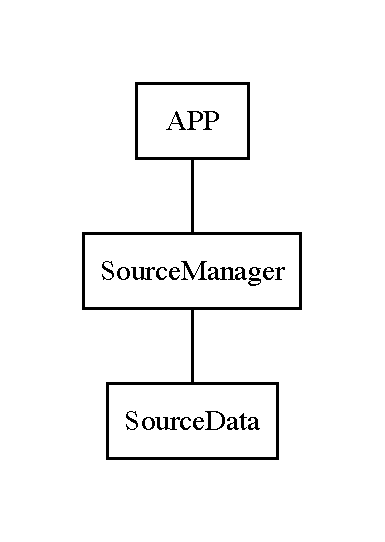
\includegraphics{graphviz-8ae89fd08ac2fd1f7bd8986e95108909e98b122b.pdf}

Aquesta arquitectura ocupa 4 capes:
\begin{enumerate}
\item {} 
Aplicació

\item {} 
Protocol

\item {} 
Adquisició

\item {} 
Dispositiu

\end{enumerate}

Els elements de twain ocupen aquestes capes tal com mostra la següent figura:

\noindent{\hspace*{\fill}\sphinxincludegraphics{{twain_layers}.png}\hspace*{\fill}}

Cada capa es descriu en les seccions que segueixen.


\subsubsection{Aplicació}
\label{\detokenize{index:aplicacio}}
En aquesta capa s'executa el software d'aplicació d'usuari.
Twain defineix les directrius de la interfície d'usuari per desenvolupar
aplicacions respecte a com accedir a les funcionalitats de twain, però
en cap moment marca com implementar l'aplicació, sinó com interactuar amb
twain.


\subsubsection{Protocol}
\label{\detokenize{index:protocol}}
El llenguatge parlat i la sintaxis utilitzada per twain. Implementa les comunicacions
per cada transferència de dades.
La capa de protocol inclou:
\begin{itemize}
\item {} 
Interfície de comunicació entre el software i twain

\item {} 
Administració de Source Manager

\item {} 
Administració dels Source Data

\end{itemize}


\subsubsection{Adquisició}
\label{\detokenize{index:adquisicio}}
Els dispositius d'adquisició poden ser físics (p.ex: escàner) o lògics (p.ex: una imatges de base de dades).
Els elements de software per controlar aquests dispositius s'anomenen fonts i són els membres
principals d'aquesta capa. Aquesta capa presenta opcionalment una interfície d'usuari de control
del dispositiu. També es pot presentar una propia interfície d'usuari, o simplement cap.
En aquest projecte s'utilitzen vàries formes de fer-ho.


\subsubsection{Dispositiu}
\label{\detokenize{index:dispositiu}}
És on resideixen els drivers dels dispositius. Converteixen els dispositius específics de hardware
en accions específiques pel dispositiu en particular. És una traducció HW-SW. Les aplicacions
que utilitzen twain no necessiten enviar els controladors del dispositiu, ja que són part de la font (Source Data),
però si que permet treballar directament amb ells.


\subsubsection{Interfície}
\label{\detokenize{index:interficie}}
Quan es construeix un software que utilitza twain, el procés d'adquisició és similar al
de la figura:

\noindent{\hspace*{\fill}\sphinxincludegraphics{{twain_userinterface}.png}\hspace*{\fill}}


\subsection{Ajuda de twain en el projecte}
\label{\detokenize{index:ajuda-de-twain-en-el-projecte}}
El que proposa la figura vista anteriorment és que l'aplicació parli directament amb el SourceManager. El
que es proposa és obrir un SourceManager, aquesta interfície permet llistar els source data, obtenir
disponibilitat i característiques dels source data, definir el sistema de finestres a utilitzar... Amb
aquest Source Manager es pot obrir i treballar directament amb un varis Source Data.

Per veure un exemple molt bàsic d'utilització, primer fixem-nos en el següent codi:

\begin{sphinxVerbatim}[commandchars=\\\{\}]
\PYG{k+kn}{import} \PYG{n+nn}{twain}
\PYG{n}{sm} \PYG{o}{=} \PYG{n}{twain}\PYG{o}{.}\PYG{n}{SourceManager}\PYG{p}{(}\PYG{l+m+mi}{0}\PYG{p}{)}
\PYG{n}{sd} \PYG{o}{=} \PYG{n}{sm}\PYG{o}{.}\PYG{n}{open\PYGZus{}source}\PYG{p}{(}\PYG{p}{)}
\end{sphinxVerbatim}

Aquest tall de codi importa la llibreria, obté un Source Manager, i llança un prompt a l'usuari
per seleccionar l'escàner amb el qual vol treballar. Òbviament és un exemple molt bàsic \sphinxquotedblleft{}d'instanciació\sphinxquotedblright{}
per començar a treballar amb un escàner, i el mètode de creació d'un Source Manager permet moltes opcions
de configuració com el nivell de finestres, el protocol... I el source data compta amb molts més detalls.

\sphinxstylestrong{nota}: A partir d'aquest punt sm = Source Manager, sd = Source Data.

Per una explicació bàsica, cal apuntar que sempre obrirem un Source Manager per treballar, i si és el cas
d'obrir un Data Source, és convenient tancar-lo a l'hora d'utilitzar-ne un altre, o quan s'ha acabat
de treballar. Seguint en l'exemple anterior:

\begin{sphinxVerbatim}[commandchars=\\\{\}]
\PYG{n}{sm}\PYG{o}{.}\PYG{n}{close}\PYG{p}{(}\PYG{p}{)}
\PYG{n}{sm}\PYG{o}{.}\PYG{n}{destroy}\PYG{p}{(}\PYG{p}{)}
\end{sphinxVerbatim}

Aquests dos mètodes permeten tancar el Source Data.
És important comentar que twain treballa amb el sistema d'estats comentat anteriorment,
i que per tant és molt important respectar l'ordre i les normes per canviar d'un estat
a un altre. Altrament la llibreria llança una excepció d'error de seqüència.


\subsubsection{Obtenir una llista de Source Data}
\label{\detokenize{index:obtenir-una-llista-de-source-data}}
Ex:

\begin{sphinxVerbatim}[commandchars=\\\{\}]
\PYG{n}{sm}\PYG{o}{.}\PYG{n}{GetSourcesList}\PYG{p}{(}\PYG{p}{)}
\end{sphinxVerbatim}

Retorn: \sphinxcode{{[}{]}} o \sphinxcode{Exception: TWCC\_NODS}
Retorna una llista de source datas o una excepció si no hi han Data Sources disponibles.


\subsubsection{Adquisició}
\label{\detokenize{index:id1}}
Hi han diverses maneres d'obtenir imatges des de la llibreria de twain, principalment
en el projecte s'han enfocat 3 de diferents, algunes més complexes d'altres.
A tall d'exemple es comenta una de les més bàsiques, pressuposant que en l'estat de l'aplicació
està en un nivell correcte, que els estats de twain romanen en el punt adient, que els Data
Sources tenen les dlls necessàries per treballar, que tenim un DSM instal·lat, que hem
configurat un Source Manager... Com es pot comprovar el procés d'interacció amb twain és
complicat i farragós. Presuposant tot això i un munt de coses més vegem-ne un exemple bàsic

\begin{sphinxVerbatim}[commandchars=\\\{\}]
\PYG{n}{sm}\PYG{o}{.}\PYG{n}{open\PYGZus{}source}\PYG{p}{(}\PYG{n}{sm}\PYG{o}{.}\PYG{n}{GetSourcesList}\PYG{p}{(}\PYG{p}{)}\PYG{p}{[}\PYG{l+m+mi}{0}\PYG{p}{]}\PYG{p}{)}
\PYG{n}{sd}\PYG{o}{.}\PYG{n}{RequestAcquire}\PYG{p}{(}\PYG{l+m+mi}{1}\PYG{p}{,} \PYG{l+m+mi}{0}\PYG{p}{)}
\PYG{n}{rv} \PYG{o}{=} \PYG{n}{sd}\PYG{o}{.}\PYG{n}{XferImageNatively}\PYG{p}{(}\PYG{p}{)}

\PYG{k}{if} \PYG{n}{rv}\PYG{p}{:}
    \PYG{p}{(}\PYG{n}{handle}\PYG{p}{,} \PYG{n}{count}\PYG{p}{)} \PYG{o}{=} \PYG{n}{rv}
\PYG{n}{twain}\PYG{o}{.}\PYG{n}{DIBToBMFile}\PYG{p}{(}\PYG{n}{handle}\PYG{p}{,} \PYG{n}{path}\PYG{p}{)}
\PYG{n}{ret\PYGZus{}value} \PYG{o}{=} \PYG{n}{handle}

\PYG{n}{sm}\PYG{o}{.}\PYG{n}{close}\PYG{p}{(}\PYG{p}{)}
\PYG{n}{sm}\PYG{o}{.}\PYG{n}{destroy}\PYG{p}{(}\PYG{p}{)}
\PYG{n}{sd}\PYG{o}{.}\PYG{n}{close}\PYG{p}{(}\PYG{p}{)}
\PYG{n}{sd}\PYG{o}{.}\PYG{n}{destroy}\PYG{p}{(}\PYG{p}{)}
\PYG{p}{(}\PYG{n}{sm}\PYG{p}{,} \PYG{n}{sd}\PYG{p}{)} \PYG{o}{=} \PYG{p}{(}\PYG{k+kc}{None}\PYG{p}{,} \PYG{k+kc}{None}\PYG{p}{)}
\end{sphinxVerbatim}

Un resum ràpid de què aconsegueix aquest tall de codi és: obrir una font i fer peticions
twain per fer una adquisició. Existeixen varis tipus de peticions, en aquest exemple es
fa una petició d'adquisició mostrant un prompt a l'usuari, i s'indica a twain que l'aplicació
està llesta per digitalitzar. Cal anotar que és vital respectar sempre els estats de twain.
Com aquesta hi han moltíssimes formes de fer una adquisició. També es poden utilitzar \sphinxstyleemphasis{callbacks}
i subscriren-s a twain, i rebre informació dels events o canvis d'estat a través d'ells.
Per certs motius com la digitalització nativa, la digitalització sense controladors o amb preferències,
s'han utilitzat diversos mètodes per l'adquisició de documents. En aquesta part no es contempla,
però la llibreria twain pot ser tan aprofundida com es vulgui, i s'han utilitzat moltes
funcions per utilitzar preferències d'escaneig, formats...


\subsubsection{Subscripció d'events}
\label{\detokenize{index:subscripcio-d-events}}
Permet subscriure's als events o canvis d'estat:

\begin{sphinxVerbatim}[commandchars=\\\{\}]
\PYG{k}{def} \PYG{n+nf}{subscribe\PYGZus{}twain}\PYG{p}{(}\PYG{n}{event}\PYG{p}{)}\PYG{p}{:}
    \PYG{k}{try}\PYG{p}{:}
        \PYG{k}{if} \PYG{n}{event} \PYG{o}{==} \PYG{n}{twain}\PYG{o}{.}\PYG{n}{MSG\PYGZus{}XFERREADY}\PYG{p}{:}
            \PYG{n}{sd}\PYG{o}{.}\PYG{n}{ProcessXFer}\PYG{p}{(}\PYG{p}{)}
        \PYG{k}{elif} \PYG{n}{event} \PYG{o}{==} \PYG{n}{twain}\PYG{o}{.}\PYG{n}{MSG\PYGZus{}CLOSEDSREQ}\PYG{p}{:}
            \PYG{n}{sd}\PYG{o}{.}\PYG{n}{close}\PYG{p}{(}\PYG{p}{)}
            \PYG{n}{sd}\PYG{o}{.}\PYG{n}{destroy}\PYG{p}{(}\PYG{p}{)}
            \PYG{n}{sd} \PYG{o}{=} \PYG{k+kc}{None}
    \PYG{k}{except}\PYG{p}{:}
        \PYG{k+kn}{import} \PYG{n+nn}{sys}\PYG{o}{,} \PYG{n+nn}{traceback}
        \PYG{n}{ei} \PYG{o}{=} \PYG{n}{sys}\PYG{o}{.}\PYG{n}{exc\PYGZus{}info}\PYG{p}{(}\PYG{p}{)}
        \PYG{n}{traceback}\PYG{o}{.}\PYG{n}{print\PYGZus{}exception}\PYG{p}{(}\PYG{n}{ei}\PYG{p}{[}\PYG{l+m+mi}{0}\PYG{p}{]}\PYG{p}{,} \PYG{n}{ei}\PYG{p}{[}\PYG{l+m+mi}{1}\PYG{p}{]}\PYG{p}{,} \PYG{n}{ei}\PYG{p}{[}\PYG{l+m+mi}{2}\PYG{p}{]}\PYG{p}{)}

\PYG{n}{sm}\PYG{o}{.}\PYG{n}{SetCallback}\PYG{p}{(}\PYG{n+nb+bp}{self}\PYG{o}{.}\PYG{n}{subscribe\PYGZus{}twain}\PYG{p}{)}
\end{sphinxVerbatim}

Es pot subscriure a qualsevol nivell de missatges. És interessant, ja que twain
està molt acostumat en treballar amb l'ús d'excepcions. I en el marc d'aquest treball,
s'han de controlar totes les possibles accions o previsions, encara que siguin d'usuari.
A tall d'exemple imaginem-nos que l'usuari cancela la digitalització, o tanca l'escàner, o...
Twain envia informació a nivell d'excepcions, i per tant l'aplicació podria deixar de funcionar
en qualsevol moment. Per tant aquesta funció ajuda molt a controlar el que ha de fer a cada cas,
altrament la casuística augmenta considerablement, fent que sigui complicat contemplar el
gran nombre de casos. Cal fer notar que en aquest TFG no només s'utilitza twain per digitalitzar, sinó per un munt
de coses més, definir preferències, obrir Data Sources, analitzar compatibilitats amb twain,
explorar característiques dels Data Sources, anàlisis de versions...
Òbviament existeixen altres maneres de subscriure's als events o capturar-los.


\subsubsection{Capabilities}
\label{\detokenize{index:capabilities}}
Existeixen diversos tipus de capabilities per configurar característiques amb la següent nomenclatura:
\begin{itemize}
\item {} 
CAP: Capabilities Generals

\item {} 
ICAP: Capabilities d'Imatge

\item {} 
ACAP: Capabilities d'Audio

\end{itemize}

Comprovar capabilities:

la funció \sphinxstyleemphasis{GetCapability} permet analitzar una propietat específica segons un Source Data donat:

\begin{sphinxVerbatim}[commandchars=\\\{\}]
\PYG{n+nb+bp}{self}\PYG{o}{.}\PYG{n}{sd}\PYG{o}{.}\PYG{n}{GetCapability}\PYG{p}{(}\PYG{n}{twain}\PYG{o}{.}\PYG{n}{ICAP\PYGZus{}PIXELTYPE}\PYG{p}{)}
\end{sphinxVerbatim}

Aquesta funció s'utilitza per retornar l'informació de la capability del Data Source. Si no s'admet la capability retorna una excepció. El tipus de retorn és:

\begin{sphinxVerbatim}[commandchars=\\\{\}]
\PYG{n}{Tupla} \PYG{k}{del} \PYG{n}{tipus} \PYG{p}{(}\PYG{n}{TWTY\PYGZus{}} \PYG{o}{*}\PYG{p}{)} \PYG{n}{i} \PYG{n}{un} \PYG{n}{valor}\PYG{o}{.}
\end{sphinxVerbatim}

El format dels valors depèn del tipus de contenidor. Les caps poden estar en els següents:

\begin{sphinxVerbatim}[commandchars=\\\{\}]
\PYG{n}{singleton}\PYG{p}{,} \PYG{n+nb}{range}\PYG{p}{,} \PYG{n}{enumerator} \PYG{o+ow}{or} \PYG{n}{array}
\end{sphinxVerbatim}

ex:

\begin{sphinxVerbatim}[commandchars=\\\{\}]
\PYG{p}{(}\PYG{l+m+mi}{1}\PYG{p}{,} \PYG{p}{(}\PYG{l+m+mi}{0}\PYG{p}{,} \PYG{l+m+mi}{0}\PYG{p}{,} \PYG{p}{[}\PYG{l+m+mi}{1}\PYG{p}{,} \PYG{l+m+mi}{2}\PYG{p}{,} \PYG{l+m+mi}{4}\PYG{p}{]}\PYG{p}{)}
\end{sphinxVerbatim}

L'últim array indica els valors permesos de la capability. Seguint l'exemple els valors assignables a la capability són: TWPT\_BW, TWPT\_GRAY, TWPT\_PDF, ja que 1, 2, 4 són el valor
d'aquestes respectivament

CAPS:

\begin{sphinxVerbatim}[commandchars=\\\{\}]
\PYG{n}{twain}\PYG{o}{.}\PYG{n}{TWPT\PYGZus{}BW}
\PYG{n}{twain}\PYG{o}{.}\PYG{n}{TWPT\PYGZus{}GRAY}
\PYG{n}{twain}\PYG{o}{.}\PYG{n}{TWPT\PYGZus{}RGB}
\end{sphinxVerbatim}


\section{PyQt}
\label{\detokenize{index:pyqt}}
Per presentar una vista de l'aplicació s'ha utilitzat l'entorn de treball PyQt, que implementa
els estàndards Qt amb Python.
Qt està fet amb C++, i PyQt permet la utilització de Qt amb el llenguatge Python.

És interessant escollir un bon sistema de vista o GUI. Les raons perqué s'ha escollit Qt són les
següents:
\begin{itemize}
\item {} 
Multisistema

\item {} 
Utilitza elements natius de cada sistema *

\item {} 
Fitxer xml per estils

\item {} 
Software de designer

\item {} 
Molta documentació

\item {} 
Suport

\end{itemize}
\begin{itemize}
\item {} 
Utilitza els elements de finestres, estils colors... de cada sistema

\end{itemize}

A part del gran suport que té Qt, s'utilitza per desenvolupar software fiable i que s'ha
anat fent popular. S'utilitza per dissenyar smart tv's, ordinadors a bord d'alguns
cotxes, smartwatches i per descomptat aplicacions, moltes aplicacions. Si els més grans
l'l'escullen, serà per alguna cosa. I els avantatges que s'han analitzat per utilitzar
Qt com a sistema GUI en són moltes, algunes esmentades a la llista anterior.

Òbviament PyQt té molta documentació com s'ha esmentat, però a més a més és una gran sort que,
sigui un sistema tant utilitzat, ja que de forma molt ràpid algú et pot donar suport. D'exemple
es pot veure la Issue que es va obrir per un dubte d'aquest projecte, i que es va resoldre de
forma molt ràpida:

\sphinxurl{https://stackoverflow.com/questions/43913716/pyqt5-focus-qmainwindow-as-first-window}

Quan es desenvolupa en un sistema GUI, el mètode de treball sol ser similar per tots, però el que
el fa característic, és la facilitat o no d'accés, i la visibilitat.

\sphinxstylestrong{Fitxers .ui}: La responsabilitat més important del programador és que la vista sigui funcional,
queda més en segon pla o com a segona tasca el disseny. Prenent més importància la funcionalitat
dels elements i menys el disseny de tals. Això és degut a que un element p.ex: del tipus botó,
pot ser molt agradable per la vista, però si no fa res, o no funciona, o no fa el que hauria
de fer, no serveix per res. Per tant interessa centrar-se més en la funcionalitat, i una de les
eines que es poden utilitzar en PyQt és \sphinxstyleemphasis{QtDesigner}, que abstreu al programador de dissenyar una
interfície de vista purament per codi, sinó que permet dissenyar a mode gràfic una vista agradable,
i posteriorment carregar-la al programa i encarregar-se de la funcionalitat dels elements ara si
via codi.

PyQt treballa amb una herència molt definida, posa a la disposició elements abstractes, i elements
cada cop a nivell més concret que hereden d'aquests primers.

Existeixen varies versions de PyQt, i un dels canvis més notoris entre versions és la separació
dels \sphinxstyleemphasis{packages}. S'ha utilitzat la versió 5. Els elements de Qt es divideixen en 4 grans \sphinxstyleemphasis{packages}
segons l'accés i la funcionalitat:
\begin{itemize}
\item {} 
Core: nucli de Qt, accés a característiques i definició de posicionats d'elements...

\item {} 
Ui: accés a fitxers .ui, i càrrega dels mateixos

\item {} 
Gui: accés a interfície bàsica, i pintat de marcs

\item {} 
Widgets: accés a elements visuals de la vista (botons, menús, layouts...)

\end{itemize}

PyQt treballa amb una estructura de comunicació típica de les GUI's. Els usuaris produeixen una acció,
l'element capta tal acció i reacciona. Aquesta metodologia es sol treballar a través de callbacks i senyals.
A PyQt es parla de senyals i slots.
\begin{itemize}
\item {} 
Senyals: són les senyals que emeten els elements al produir-se una acció

\item {} 
Slots: són les funcions que es connecten a les senyals

\end{itemize}

connexió de botons: com s'ha mencionat abans, podem connectar elements de la vista amb accions. L'acció del clic d'un botó es connecta a una funció de la seguent manera:

\begin{sphinxVerbatim}[commandchars=\\\{\}]
\PYG{n+nb+bp}{self}\PYG{o}{.}\PYG{n}{name\PYGZus{}button}\PYG{o}{.}\PYG{n}{clickec}\PYG{o}{.}\PYG{n}{connect}\PYG{p}{(}\PYG{n+nb+bp}{self}\PYG{o}{.}\PYG{n}{name\PYGZus{}function}\PYG{p}{)}
\end{sphinxVerbatim}

Pot ser interessant conèixer propietats del botò o reaprofitar una funció en varis botons.
Podem fer ús del self.sender()
En aquest exemple pràctic es mostra com determinar quin botò ha enviat la senyal

\begin{sphinxVerbatim}[commandchars=\\\{\}]
\PYG{n+nb+bp}{self}\PYG{o}{.}\PYG{n}{button\PYGZus{}1}\PYG{o}{.}\PYG{n}{clicked}\PYG{o}{.}\PYG{n}{connect}\PYG{p}{(}\PYG{n+nb+bp}{self}\PYG{o}{.}\PYG{n}{name\PYGZus{}function}\PYG{p}{)}
\PYG{n+nb+bp}{self}\PYG{o}{.}\PYG{n}{button\PYGZus{}2}\PYG{o}{.}\PYG{n}{clicked}\PYG{o}{.}\PYG{n}{connect}\PYG{p}{(}\PYG{n+nb+bp}{self}\PYG{o}{.}\PYG{n}{name\PYGZus{}function}\PYG{p}{)}

\PYG{k}{def} \PYG{n+nf}{name\PYGZus{}function}\PYG{p}{(}\PYG{n+nb+bp}{self}\PYG{p}{)}\PYG{p}{:}
    \PYG{n+nb}{print}\PYG{p}{(}\PYG{n+nb+bp}{self}\PYG{o}{.}\PYG{n}{sender}\PYG{p}{(}\PYG{p}{)}\PYG{p}{)}
\end{sphinxVerbatim}

També es permet passar paràmetres directament amb l'ús de les lambdes de python

\begin{sphinxVerbatim}[commandchars=\\\{\}]
self.button\PYGZus{}1.clicked.connect(lambda: self.name\PYGZus{}function(1))
self.button\PYGZus{}2.clicked.connect(lambda: self.name\PYGZus{}function(2))

def name\PYGZus{}function(self, numer):
    print(“Button “, number, “ clicked”)
\end{sphinxVerbatim}

Altres elements com Combobox, TableView, ListView... es poden connectar a senyals.
Combobox: ens serà interessant saber quan i si hem canviat un element del nostre combobox.

Sovint és interessant realitzar un procés de \sphinxstyleemphasis{customització} de una GUI mitjançant codi. PyQt posa a disposició una sèrie de funcions per tal de estilitzar una vista. Cuidant molt l’herència i delegant responsabilitats s’ofereixen mètodes per afegir, decorar, eliminar... components.
Cada canvi té assignat un responsable, és a dir que el canvi de un component s’haurà de fer sobre el mateix. Un possible exemple és el que segueix: Quan s’intenta canviar
el \sphinxstyleemphasis{header} d’una taula, s’atacarà directament sobre aquest \sphinxstyleemphasis{header} i no sobre la taula. A continuació es detalla en aquest fragment de codi:

\begin{sphinxVerbatim}[commandchars=\\\{\}]
\PYG{n+nb+bp}{self}\PYG{o}{.}\PYG{n}{table\PYGZus{}name}\PYG{p}{(}\PYG{p}{)}
\PYG{n+nb+bp}{self}\PYG{o}{.}\PYG{n}{table\PYGZus{}name}\PYG{o}{.}\PYG{n}{horizontalHeader}\PYG{p}{(}\PYG{p}{)}\PYG{o}{.}\PYG{n}{setSectionResizeMode}\PYG{p}{(}\PYG{n}{QHeaderView}\PYG{o}{.}\PYG{n}{Fixed}\PYG{p}{)}
\end{sphinxVerbatim}

En l'exemple vist, es canvia el mode en el qual els elements d'un \sphinxstyleemphasis{header} canvien de tamany. En aquest cas es posa a fixed, fent que l'usuari no pugui fer \sphinxstyleemphasis{resize} directament a la vista. Però l'interessant és veure com es deleguen les responsabilitats als elements de Qt. Com que es canvia una propietat del \sphinxstyleemphasis{header} s'ataca directament al \_horitzontalHeader\_, y no a la taula. I la propietat corresponent
és pertanyent a la vista d'un header, per tant es passa a la funció un element del tipus QHeaderView.

PyQt té un munt de coses interessants, per exemple a comentar. En aquest software s'utilitza una icona
de sistema per donar un feedback a l'usuari de que el programa està corrent i que tot està correcte. PyQt
posa a la disposició un SystrayIcon.


\section{ØMQ}
\label{\detokenize{index:omq}}
Després d'un estudi i petit disseny de la comunicació, es va decidir utilitzar sockets per
una comunicació del tipus IPC.
El llenguatge Python incorpora una llibreria de sockets, però ja que aquest projecte té previsió
de desplegar-se en diverses empreses, dins de les quals es mouran forces dades, les mètriques
de temps podrien augmentar considerablement. I una bona solució és utilitzar una plataforma
per la comunicació via sockets molt ràpida.

ØMQ és una plataforma que segons \sphinxurl{http://zeromq.org/} permet:
\begin{itemize}
\item {} 
Connectar el codi en qualsevol llenguatge i en qualsevol sistema.

\item {} 
Utilitzar les arquitectures: IPC, TCP, TIPC, i multicast.

\item {} 
Ús de patrons pub-sub, push-pull i router-dealer.

\item {} 
Motors E/S asíncrons d'alta velocitat

\item {} 
Construir qualsevol arquitectura: centralitzada, distribuïda, petita o gran.

\item {} 
Software lliure

\end{itemize}

Es proposa la meto socket-client i també la creació d'un socket PUBLISHER, i
altres SUBSCRIBERS, que es subscriuren a aquest PUBLISHER, però que a més es poden subscriure
a certs nivells de missatges, i per tant els sockets SUBSCRIBER només recolliran els
missatges necessaris.

És interessant en aquest treball utilitzar dues metodologies de sockets, que en propers
capítols es detallaran.
Un d'estructura client - servidor, i l'altre publisher-subscibers

\noindent{\hspace*{\fill}\sphinxincludegraphics[scale=0.7]{{zmq}.png}\hspace*{\fill}}

ØMQ conegut també per zmq, facilita molt l'enviament de dades en format tipus JSON. Actualment s'està tornant
un format molt estàndard, i zmq dóna les facilitats d'enviar un paquet en del tipus, string,
llista, diccionari... i parsejar-ho com a JSON. A l'altre banda del socket es podrà rebre
en el format que es necessiti. És un avantatge poder fer una bona abstracció de dades
gràcies a facilitats com la d'enviament de dades en format JSON, ja que no tots els sockets
en altres versions no ho permeten o és de difícil utilització.

El llenguatge Python pot incorporar la llibreria \sphinxcode{pyzmq} que proporciona l'ús i l'accés
a zmq.

Anteriorment s'ha comentat que són dos les arquitectures de sockets que s'utilitzaran en
aquest projecte. A mode d'exemple a continuació es mostra la creació d'un socket \sphinxstylestrong{REP}
d'arquitectura REQ - REP, que s'ha utilitzat en el projecte:

\sphinxstylestrong{Nota:} El següent bloc de codi utilitza la importació de @IP, \#PORT i Protocol des d'un
fitxer de configuració, per tal de que sigui més fàcil la configuració i el despleguement de
l'aplicació en diferents entorns.

\begin{sphinxVerbatim}[commandchars=\\\{\}]
\PYG{k+kn}{import} \PYG{n+nn}{configparser}
\PYG{k+kn}{import} \PYG{n+nn}{pyzmq}

\PYG{n+nd}{@property}
\PYG{k}{def} \PYG{n+nf}{route}\PYG{p}{(}\PYG{n+nb+bp}{self}\PYG{p}{)}\PYG{p}{:}
    \PYG{n}{parser} \PYG{o}{=} \PYG{n}{configparser}\PYG{o}{.}\PYG{n}{ConfigParser}\PYG{p}{(}\PYG{p}{)}
    \PYG{n}{parser}\PYG{o}{.}\PYG{n}{read}\PYG{p}{(}\PYG{l+s+s1}{\PYGZsq{}}\PYG{l+s+s1}{config.cfg}\PYG{l+s+s1}{\PYGZsq{}}\PYG{p}{)}
    \PYG{n}{port} \PYG{o}{=} \PYG{n}{parser}\PYG{o}{.}\PYG{n}{getint}\PYG{p}{(}\PYG{l+s+s1}{\PYGZsq{}}\PYG{l+s+s1}{PORT}\PYG{l+s+s1}{\PYGZsq{}}\PYG{p}{,} \PYG{l+s+s1}{\PYGZsq{}}\PYG{l+s+s1}{port}\PYG{l+s+s1}{\PYGZsq{}}\PYG{p}{)}
    \PYG{n}{ip} \PYG{o}{=} \PYG{n}{parser}\PYG{o}{.}\PYG{n}{items}\PYG{p}{(}\PYG{l+s+s1}{\PYGZsq{}}\PYG{l+s+s1}{HOST}\PYG{l+s+s1}{\PYGZsq{}}\PYG{p}{)}\PYG{p}{[}\PYG{l+m+mi}{0}\PYG{p}{]}\PYG{p}{[}\PYG{l+m+mi}{1}\PYG{p}{]}
    \PYG{n}{protocol} \PYG{o}{=} \PYG{n}{parser}\PYG{o}{.}\PYG{n}{items}\PYG{p}{(}\PYG{l+s+s1}{\PYGZsq{}}\PYG{l+s+s1}{PROTOCOL}\PYG{l+s+s1}{\PYGZsq{}}\PYG{p}{)}\PYG{p}{[}\PYG{l+m+mi}{0}\PYG{p}{]}\PYG{p}{[}\PYG{l+m+mi}{1}\PYG{p}{]}

    \PYG{k}{return} \PYG{l+s+s1}{\PYGZsq{}}\PYG{l+s+si}{\PYGZob{}0\PYGZcb{}}\PYG{l+s+s1}{://}\PYG{l+s+si}{\PYGZob{}1\PYGZcb{}}\PYG{l+s+s1}{:}\PYG{l+s+si}{\PYGZob{}2\PYGZcb{}}\PYG{l+s+s1}{\PYGZsq{}}\PYG{o}{.}\PYG{n}{format}\PYG{p}{(}\PYG{n}{protocol}\PYG{p}{,} \PYG{n}{ip}\PYG{p}{,} \PYG{n}{port}\PYG{p}{)}

\PYG{k}{def} \PYG{n+nf}{sock\PYGZus{}connect}\PYG{p}{(}\PYG{n+nb+bp}{self}\PYG{p}{)}\PYG{p}{:}
    \PYG{n}{context} \PYG{o}{=} \PYG{n}{zmq}\PYG{o}{.}\PYG{n}{Context}\PYG{p}{(}\PYG{p}{)}
    \PYG{n+nb+bp}{self}\PYG{o}{.}\PYG{n}{publisher} \PYG{o}{=} \PYG{n}{context}\PYG{o}{.}\PYG{n}{socket}\PYG{p}{(}\PYG{n}{zmq}\PYG{o}{.}\PYG{n}{PUB}\PYG{p}{)}
    \PYG{n+nb+bp}{self}\PYG{o}{.}\PYG{n}{publisher}\PYG{o}{.}\PYG{n}{bind}\PYG{p}{(}\PYG{n+nb+bp}{self}\PYG{o}{.}\PYG{n}{route}\PYG{p}{)}
\end{sphinxVerbatim}


\section{SQLite}
\label{\detokenize{index:sqlite}}\label{\detokenize{index:reference-sqlite}}
Cal gestionar una base de dades per guardar les preferències i els perfils que gestionin
els usuaris. SQLite (\sphinxurl{https://www.sqlite.org/}) és una base de dades relacional que proporciona l'emmagatzemament de
la base de dades en un fitxer que conté la definició de l'estructura de les taules i les dades.
Es proposa un sistema eficient i \sphinxstyleemphasis{light}, ja que es necessita una base de dades lleugera, on
el volum de dades a emmagatzemar és relativament petit. A més, no és un sistema de gestió de
base de dades que funcioni amb una metodologia client-servidor, sinó que està integrat
totalment dins el programa. Per tant a l'hora d'analitzar els requisits necessaris per la
creació i gestió de la base de dades, SQLite s'ajusta molt bé a les necessitats proposades.

Existeix una llibreria de Python anomenada sqlite3, per gestionar una base
de dades amb SQLite en aquest llenguatge. A continuació es detalla el funcionament
bàsic:

Es proposa crear un connector a la base de dades i un cursor per realitzar
operacions sobre aquesta. La base de dades està persistida en un fitxer \sphinxstylestrong{.db}.
Si la base de dades no existeix, SQLite la crea automàticament.

\begin{sphinxVerbatim}[commandchars=\\\{\}]
\PYG{k+kn}{import} \PYG{n+nn}{sqlite3}
\PYG{n}{conn} \PYG{o}{=} \PYG{n}{sqlite3}\PYG{o}{.}\PYG{n}{connect}\PYG{p}{(}\PYG{l+s+s1}{\PYGZsq{}}\PYG{l+s+s1}{foo.db}\PYG{l+s+s1}{\PYGZsq{}}\PYG{p}{)}
\PYG{n}{cursor} \PYG{o}{=} \PYG{n}{conn}\PYG{o}{.}\PYG{n}{cursor}\PYG{p}{(}\PYG{p}{)}
\end{sphinxVerbatim}

\sphinxstylestrong{Create table:}

\begin{sphinxVerbatim}[commandchars=\\\{\}]
\PYG{n}{cursor}\PYG{o}{.}\PYG{n}{execute}\PYG{p}{(}\PYG{l+s+s1}{\PYGZsq{}\PYGZsq{}\PYGZsq{}}\PYG{l+s+s1}{Create table if not exists Foo (id\PYGZus{}foo, name)}\PYG{l+s+s1}{\PYGZsq{}\PYGZsq{}\PYGZsq{}}\PYG{p}{)}
\end{sphinxVerbatim}

Amb \sphinxcode{{}`create table if not exists{}`}, ens assegurem que que no es llanci una excepció de taula
ja existent. Després de cada operació, o de varies, es graven els canvis utilitzant
el connector:

\begin{sphinxVerbatim}[commandchars=\\\{\}]
\PYG{n}{conn}\PYG{o}{.}\PYG{n}{commit}\PYG{p}{(}\PYG{p}{)}
\end{sphinxVerbatim}

\sphinxstylestrong{Inserts:} Es permeten inserts unitaris o multiregistre.

\begin{sphinxVerbatim}[commandchars=\\\{\}]
\PYG{n}{cursor}\PYG{o}{.}\PYG{n}{execute}\PYG{p}{(}\PYG{l+s+s1}{\PYGZsq{}\PYGZsq{}\PYGZsq{}}\PYG{l+s+s1}{Insert into Foo values (1, }\PYG{l+s+s1}{\PYGZsq{}}\PYG{l+s+s1}{name}\PYG{l+s+s1}{\PYGZsq{}}\PYG{l+s+s1}{)}\PYG{l+s+s1}{\PYGZsq{}\PYGZsq{}\PYGZsq{}}\PYG{p}{)}
\PYG{n}{conn}\PYG{o}{.}\PYG{n}{commit}\PYG{p}{(}\PYG{p}{)}
\PYG{n}{\PYGZus{}values} \PYG{o}{=} \PYG{p}{[}\PYG{p}{(}\PYG{l+m+mi}{1}\PYG{p}{,}\PYG{l+s+s1}{\PYGZsq{}}\PYG{l+s+s1}{name\PYGZus{}1}\PYG{l+s+s1}{\PYGZsq{}}\PYG{p}{)}\PYG{p}{,}\PYG{p}{(}\PYG{l+m+mi}{2}\PYG{p}{,}\PYG{l+s+s1}{\PYGZsq{}}\PYG{l+s+s1}{name\PYGZus{}2}\PYG{l+s+s1}{\PYGZsq{}}\PYG{p}{)}\PYG{p}{,}\PYG{p}{(}\PYG{l+m+mi}{3}\PYG{p}{,}\PYG{l+s+s1}{\PYGZsq{}}\PYG{l+s+s1}{name\PYGZus{}3}\PYG{l+s+s1}{\PYGZsq{}}\PYG{p}{)}\PYG{p}{]}
\PYG{n}{cursor}\PYG{o}{.}\PYG{n}{executemany}\PYG{p}{(}\PYG{l+s+s1}{\PYGZsq{}}\PYG{l+s+s1}{Insert into Foo values (?, ?)}\PYG{l+s+s1}{\PYGZsq{}}\PYG{p}{,}\PYG{n}{\PYGZus{}values}\PYG{p}{)}
\PYG{n}{conn}\PYG{o}{.}\PYG{n}{commit}\PYG{p}{(}\PYG{p}{)}
\end{sphinxVerbatim}

\sphinxstylestrong{Query:} Les consultes són del tipus registre unitari o multiregistre.

\begin{sphinxVerbatim}[commandchars=\\\{\}]
\PYG{n}{cursor}\PYG{o}{.}\PYG{n}{execute}\PYG{p}{(}\PYG{l+s+s1}{\PYGZsq{}\PYGZsq{}\PYGZsq{}}\PYG{l+s+s1}{select * from Foo}\PYG{l+s+s1}{\PYGZsq{}\PYGZsq{}\PYGZsq{}}\PYG{p}{)}
\PYG{n}{result} \PYG{o}{=} \PYG{n}{cursor}\PYG{o}{.}\PYG{n}{fetchone}\PYG{p}{(}\PYG{p}{)}

\PYG{n}{cursor}\PYG{o}{.}\PYG{n}{execute}\PYG{p}{(}\PYG{l+s+s1}{\PYGZsq{}\PYGZsq{}\PYGZsq{}}\PYG{l+s+s1}{select * from Foo}\PYG{l+s+s1}{\PYGZsq{}\PYGZsq{}\PYGZsq{}}\PYG{p}{)}
\PYG{n}{result} \PYG{o}{=} \PYG{n}{cursor}\PYG{o}{.}\PYG{n}{fetchmany}\PYG{p}{(}\PYG{p}{)}

\PYG{l+s+sd}{\PYGZsq{}\PYGZsq{}\PYGZsq{}equivalent al cursor.fetchmany\PYGZsq{}\PYGZsq{}\PYGZsq{}}
\PYG{k}{for} \PYG{n}{row} \PYG{o+ow}{in} \PYG{n}{cursor}\PYG{o}{.}\PYG{n}{execute}\PYG{p}{(}\PYG{l+s+s1}{\PYGZsq{}\PYGZsq{}\PYGZsq{}}\PYG{l+s+s1}{Select * from Foo}\PYG{l+s+s1}{\PYGZsq{}\PYGZsq{}\PYGZsq{}}\PYG{p}{)}\PYG{p}{:}
    \PYG{n+nb}{print}\PYG{p}{(}\PYG{n}{row}\PYG{p}{)}
\end{sphinxVerbatim}

Vegem-ne una petita utilització en el projecte:

\begin{sphinxVerbatim}[commandchars=\\\{\}]
\PYG{k}{def} \PYG{n+nf}{insert\PYGZus{}one}\PYG{p}{(}\PYG{n+nb+bp}{self}\PYG{p}{,} \PYG{n}{field}\PYG{p}{,} \PYG{n}{value}\PYG{p}{)}\PYG{p}{:}
    \PYG{k}{try}\PYG{p}{:}
        \PYG{n}{query} \PYG{o}{=} \PYG{l+s+s1}{\PYGZsq{}}\PYG{l+s+si}{\PYGZob{}0\PYGZcb{}}\PYG{l+s+si}{\PYGZob{}1\PYGZcb{}}\PYG{l+s+si}{\PYGZob{}2\PYGZcb{}}\PYG{l+s+si}{\PYGZob{}3\PYGZcb{}}\PYG{l+s+si}{\PYGZob{}4\PYGZcb{}}\PYG{l+s+s1}{\PYGZsq{}}\PYG{o}{.}\PYG{n}{format}\PYG{p}{(}\PYG{l+s+s1}{\PYGZsq{}\PYGZsq{}\PYGZsq{}}\PYG{l+s+s1}{Insert into preferences (}\PYG{l+s+s1}{\PYGZsq{}\PYGZsq{}\PYGZsq{}}\PYG{p}{,} \PYG{n}{field}\PYG{p}{,} \PYG{l+s+s1}{\PYGZsq{}\PYGZsq{}\PYGZsq{}}\PYG{l+s+s1}{) values(}\PYG{l+s+s1}{\PYGZdq{}}\PYG{l+s+s1}{\PYGZsq{}\PYGZsq{}\PYGZsq{}}\PYG{p}{,} \PYG{n}{value}\PYG{p}{,} \PYG{l+s+s1}{\PYGZsq{}\PYGZsq{}\PYGZsq{}}\PYG{l+s+s1}{\PYGZdq{}}\PYG{l+s+s1}{)}\PYG{l+s+s1}{\PYGZsq{}\PYGZsq{}\PYGZsq{}}\PYG{p}{)}
        \PYG{n+nb+bp}{self}\PYG{o}{.}\PYG{n}{cursor}\PYG{o}{.}\PYG{n}{execute}\PYG{p}{(}\PYG{n}{query}\PYG{p}{)}
        \PYG{n+nb+bp}{self}\PYG{o}{.}\PYG{n}{conn}\PYG{o}{.}\PYG{n}{commit}\PYG{p}{(}\PYG{p}{)}

        \PYG{n+nb+bp}{self}\PYG{o}{.}\PYG{n}{logger}\PYG{o}{.}\PYG{n}{info}\PYG{p}{(}\PYG{n+nb+bp}{self}\PYG{o}{.}\PYG{n}{cursor}\PYG{o}{.}\PYG{n}{execute}\PYG{p}{(}\PYG{l+s+s1}{\PYGZsq{}}\PYG{l+s+s1}{select * from preferences}\PYG{l+s+s1}{\PYGZsq{}}\PYG{p}{)}\PYG{o}{.}\PYG{n}{fetchone}\PYG{p}{(}\PYG{p}{)}\PYG{p}{)}
    \PYG{k}{except} \PYG{n}{sqlite3}\PYG{o}{.}\PYG{n}{OperationalError}\PYG{p}{:}
        \PYG{n+nb+bp}{self}\PYG{o}{.}\PYG{n}{logger}\PYG{o}{.}\PYG{n}{info}\PYG{p}{(}\PYG{l+s+s1}{\PYGZsq{}}\PYG{l+s+s1}{\PYGZsh{}\PYGZsh{}\PYGZsh{}\PYGZsh{}\PYGZsh{}\PYGZsh{}\PYGZsh{} NO INSERT FIELD}\PYG{l+s+s1}{\PYGZsq{}}\PYG{p}{)}

\PYG{k}{def} \PYG{n+nf}{update\PYGZus{}one}\PYG{p}{(}\PYG{n+nb+bp}{self}\PYG{p}{,} \PYG{n}{field}\PYG{p}{,} \PYG{n}{value}\PYG{p}{)}\PYG{p}{:}
    \PYG{k}{try}\PYG{p}{:}
        \PYG{n}{query} \PYG{o}{=} \PYG{l+s+s1}{\PYGZsq{}}\PYG{l+s+si}{\PYGZob{}0\PYGZcb{}}\PYG{l+s+si}{\PYGZob{}1\PYGZcb{}}\PYG{l+s+si}{\PYGZob{}2\PYGZcb{}}\PYG{l+s+si}{\PYGZob{}3\PYGZcb{}}\PYG{l+s+si}{\PYGZob{}4\PYGZcb{}}\PYG{l+s+s1}{\PYGZsq{}}\PYG{o}{.}\PYG{n}{format}\PYG{p}{(}\PYG{l+s+s1}{\PYGZsq{}\PYGZsq{}\PYGZsq{}}\PYG{l+s+s1}{update preferences set }\PYG{l+s+s1}{\PYGZsq{}\PYGZsq{}\PYGZsq{}}\PYG{p}{,} \PYG{n}{field}\PYG{p}{,} \PYG{l+s+s1}{\PYGZsq{}\PYGZsq{}\PYGZsq{}}\PYG{l+s+s1}{=}\PYG{l+s+s1}{\PYGZdq{}}\PYG{l+s+s1}{\PYGZsq{}\PYGZsq{}\PYGZsq{}}\PYG{p}{,} \PYG{n}{value}\PYG{p}{,} \PYG{l+s+s1}{\PYGZsq{}\PYGZsq{}\PYGZsq{}}\PYG{l+s+s1}{\PYGZdq{}}\PYG{l+s+s1}{\PYGZsq{}\PYGZsq{}\PYGZsq{}}\PYG{p}{)}
        \PYG{n+nb+bp}{self}\PYG{o}{.}\PYG{n}{cursor}\PYG{o}{.}\PYG{n}{execute}\PYG{p}{(}\PYG{n}{query}\PYG{p}{)}
        \PYG{n+nb+bp}{self}\PYG{o}{.}\PYG{n}{conn}\PYG{o}{.}\PYG{n}{commit}\PYG{p}{(}\PYG{p}{)}

        \PYG{n+nb+bp}{self}\PYG{o}{.}\PYG{n}{logger}\PYG{o}{.}\PYG{n}{info}\PYG{p}{(}\PYG{n+nb+bp}{self}\PYG{o}{.}\PYG{n}{cursor}\PYG{o}{.}\PYG{n}{execute}\PYG{p}{(}\PYG{l+s+s1}{\PYGZsq{}}\PYG{l+s+s1}{select * from preferences}\PYG{l+s+s1}{\PYGZsq{}}\PYG{p}{)}\PYG{o}{.}\PYG{n}{fetchall}\PYG{p}{(}\PYG{p}{)}\PYG{p}{)}
    \PYG{k}{except} \PYG{n}{sqlite3}\PYG{o}{.}\PYG{n}{OperationalError}\PYG{p}{:}
        \PYG{n+nb+bp}{self}\PYG{o}{.}\PYG{n}{logger}\PYG{o}{.}\PYG{n}{info}\PYG{p}{(}\PYG{l+s+s1}{\PYGZsq{}}\PYG{l+s+s1}{\PYGZsh{}\PYGZsh{}\PYGZsh{}\PYGZsh{}\PYGZsh{}\PYGZsh{}\PYGZsh{} NO UPDATE FIELD}\PYG{l+s+s1}{\PYGZsq{}}\PYG{p}{)}
\end{sphinxVerbatim}


\section{cx\_Freeze}
\label{\detokenize{index:cx-freeze}}
Aquesta llibreria permet generar executables en llenguatge Python. Aquest projecte es desplegarà
en un Sistema Operatiu Windows, i \sphinxcode{{}`CX FREEZE{}`} ajuda a crear fitxers \sphinxcode{{}`.exe{}`} o instal·ladors
\sphinxcode{{}`msi{}`}.

Per utilitzar aquesta eina es pot instal·lar via pip igual com s'ha mostrat amb altres
llibreries d'aquest capítol.

\begin{sphinxVerbatim}[commandchars=\\\{\}]
\PYG{n}{pip} \PYG{n}{install} \PYG{n}{cx\PYGZus{}Freeze}
\end{sphinxVerbatim}

Aquesta eina llegeix un fitxer de setup: \sphinxcode{{}`setup.py{}`}, i genera l'executable. Per tant
cal crear un fitxer amb l'estructura que proposa cx\_Freeze.

La forma més senzilla de generar un primer setup és utilitzar la comanda:

\begin{sphinxVerbatim}[commandchars=\\\{\}]
\PYG{n}{cxfreeze}\PYG{o}{\PYGZhy{}}\PYG{n}{quickstart}
\end{sphinxVerbatim}

Ens demanarà el nom del projecte, la versió...
En realitat l'únic que fa és crear un arxiu \sphinxcode{{}`setup.py{}`} amb la versió, nom...
Però és interessant saber que en aquest fitxer s'han d'incloure totes les
dependències, paquets, paths...
Per fer-ho cal seguir l'estructura que proposa CX FREEZE.
Un cop programat el setup, només cal executar-lo amb les opcions que es necessiten:

\begin{sphinxVerbatim}[commandchars=\\\{\}]
\PYG{n}{python} \PYG{n}{setup}\PYG{o}{.}\PYG{n}{py} \PYG{p}{[}\PYG{n}{options}\PYG{p}{]}
\end{sphinxVerbatim}

Opcions interessants:

\sphinxstylestrong{Construïr un executable}:

\begin{sphinxVerbatim}[commandchars=\\\{\}]
\PYG{n}{python} \PYG{n}{setup}\PYG{o}{.}\PYG{n}{py} \PYG{n}{build}
\end{sphinxVerbatim}

\sphinxstylestrong{Construïr un instal·lador}:

\begin{sphinxVerbatim}[commandchars=\\\{\}]
\PYG{n}{python} \PYG{n}{setup}\PYG{o}{.}\PYG{n}{py} \PYG{n}{bdist\PYGZus{}msi}
\end{sphinxVerbatim}

En el projecte interessa construir un instal·lador.

Setup actual

\begin{sphinxVerbatim}[commandchars=\\\{\}]
\PYG{k+kn}{from} \PYG{n+nn}{cx\PYGZus{}Freeze} \PYG{k}{import} \PYG{n}{setup}\PYG{p}{,} \PYG{n}{Executable}
\PYG{k+kn}{import} \PYG{n+nn}{sys}
\PYG{k+kn}{import} \PYG{n+nn}{os}
\PYG{n}{base} \PYG{o}{=} \PYG{l+s+s1}{\PYGZsq{}}\PYG{l+s+s1}{Win32GUI}\PYG{l+s+s1}{\PYGZsq{}} \PYG{k}{if} \PYG{n}{sys}\PYG{o}{.}\PYG{n}{platform} \PYG{o}{==} \PYG{l+s+s1}{\PYGZsq{}}\PYG{l+s+s1}{win32}\PYG{l+s+s1}{\PYGZsq{}} \PYG{k}{else} \PYG{k+kc}{None}

\PYG{n}{shortcut\PYGZus{}table} \PYG{o}{=} \PYG{p}{[}
  \PYG{p}{(}\PYG{l+s+s2}{\PYGZdq{}}\PYG{l+s+s2}{DesktopShortcut}\PYG{l+s+s2}{\PYGZdq{}}\PYG{p}{,}           \PYG{c+c1}{\PYGZsh{} Shortcut}
   \PYG{l+s+s2}{\PYGZdq{}}\PYG{l+s+s2}{DesktopFolder}\PYG{l+s+s2}{\PYGZdq{}}\PYG{p}{,}             \PYG{c+c1}{\PYGZsh{} Directory\PYGZus{}}
   \PYG{l+s+s2}{\PYGZdq{}}\PYG{l+s+s2}{ScannerApp Connector}\PYG{l+s+s2}{\PYGZdq{}}\PYG{p}{,}      \PYG{c+c1}{\PYGZsh{} Name}
   \PYG{l+s+s2}{\PYGZdq{}}\PYG{l+s+s2}{TARGETDIR}\PYG{l+s+s2}{\PYGZdq{}}\PYG{p}{,}                 \PYG{c+c1}{\PYGZsh{} Component\PYGZus{}}
   \PYG{l+s+s2}{\PYGZdq{}}\PYG{l+s+s2}{[TARGETDIR]connector.exe}\PYG{l+s+s2}{\PYGZdq{}}\PYG{p}{,}  \PYG{c+c1}{\PYGZsh{} Target}
   \PYG{k+kc}{None}\PYG{p}{,}                        \PYG{c+c1}{\PYGZsh{} Arguments}
   \PYG{k+kc}{None}\PYG{p}{,}                        \PYG{c+c1}{\PYGZsh{} Description}
   \PYG{k+kc}{None}\PYG{p}{,}                        \PYG{c+c1}{\PYGZsh{} Hotkey}
   \PYG{k+kc}{None}\PYG{p}{,}                        \PYG{c+c1}{\PYGZsh{} Icon}
   \PYG{k+kc}{None}\PYG{p}{,}                        \PYG{c+c1}{\PYGZsh{} IconIndex}
   \PYG{k+kc}{None}\PYG{p}{,}                        \PYG{c+c1}{\PYGZsh{} ShowCmd}
   \PYG{l+s+s1}{\PYGZsq{}}\PYG{l+s+s1}{TARGETDIR}\PYG{l+s+s1}{\PYGZsq{}}                  \PYG{c+c1}{\PYGZsh{} WkDir}
   \PYG{p}{)}
  \PYG{p}{]}

\PYG{c+c1}{\PYGZsh{} Creació de la taula d\PYGZsq{}accessos}
\PYG{n}{msi\PYGZus{}data} \PYG{o}{=} \PYG{p}{\PYGZob{}}\PYG{l+s+s1}{\PYGZsq{}}\PYG{l+s+s1}{Shortcut}\PYG{l+s+s1}{\PYGZsq{}}\PYG{p}{:} \PYG{n}{shortcut\PYGZus{}table}\PYG{p}{\PYGZcb{}}

\PYG{c+c1}{\PYGZsh{} Change les opcions MSI per defecte i especifica l\PYGZsq{}ús de la taula definida}
\PYG{n}{bdist\PYGZus{}msi\PYGZus{}options} \PYG{o}{=} \PYG{p}{\PYGZob{}}\PYG{l+s+s1}{\PYGZsq{}}\PYG{l+s+s1}{data}\PYG{l+s+s1}{\PYGZsq{}}\PYG{p}{:} \PYG{n}{msi\PYGZus{}data}\PYG{p}{\PYGZcb{}}

\PYG{n}{options} \PYG{o}{=} \PYG{p}{\PYGZob{}}
  \PYG{l+s+s1}{\PYGZsq{}}\PYG{l+s+s1}{build\PYGZus{}exe}\PYG{l+s+s1}{\PYGZsq{}}\PYG{p}{:} \PYG{p}{\PYGZob{}}
      \PYG{l+s+s1}{\PYGZsq{}}\PYG{l+s+s1}{include\PYGZus{}files}\PYG{l+s+s1}{\PYGZsq{}}\PYG{p}{:} \PYG{p}{[}
          \PYG{l+s+s1}{\PYGZsq{}}\PYG{l+s+s1}{scannerapp/GUI/templates}\PYG{l+s+s1}{\PYGZsq{}}\PYG{p}{,}
          \PYG{l+s+s1}{\PYGZsq{}}\PYG{l+s+s1}{scannerapp/GUI/images}\PYG{l+s+s1}{\PYGZsq{}}\PYG{p}{,}
          \PYG{l+s+s1}{\PYGZsq{}}\PYG{l+s+s1}{scannerapp/agent/config.cfg}\PYG{l+s+s1}{\PYGZsq{}}\PYG{p}{,}
          \PYG{l+s+s1}{\PYGZsq{}}\PYG{l+s+s1}{scannerapp/GUI/images/printer.png}\PYG{l+s+s1}{\PYGZsq{}}\PYG{p}{,}
          \PYG{n}{os}\PYG{o}{.}\PYG{n}{path}\PYG{o}{.}\PYG{n}{join}\PYG{p}{(}\PYG{n}{sys}\PYG{o}{.}\PYG{n}{base\PYGZus{}prefix}\PYG{p}{,} \PYG{l+s+s1}{\PYGZsq{}}\PYG{l+s+s1}{DLLs}\PYG{l+s+s1}{\PYGZsq{}}\PYG{p}{,} \PYG{l+s+s1}{\PYGZsq{}}\PYG{l+s+s1}{sqlite3.dll}\PYG{l+s+s1}{\PYGZsq{}}\PYG{p}{)}\PYG{p}{,}
          \PYG{n}{os}\PYG{o}{.}\PYG{n}{path}\PYG{o}{.}\PYG{n}{join}\PYG{p}{(}\PYG{n}{sys}\PYG{o}{.}\PYG{n}{base\PYGZus{}prefix}\PYG{p}{,} \PYG{l+s+s1}{\PYGZsq{}}\PYG{l+s+s1}{DLLs}\PYG{l+s+s1}{\PYGZsq{}}\PYG{p}{,} \PYG{l+s+s1}{\PYGZsq{}}\PYG{l+s+s1}{tk86t.dll}\PYG{l+s+s1}{\PYGZsq{}}\PYG{p}{)}\PYG{p}{,}
          \PYG{n}{os}\PYG{o}{.}\PYG{n}{path}\PYG{o}{.}\PYG{n}{join}\PYG{p}{(}\PYG{n}{sys}\PYG{o}{.}\PYG{n}{base\PYGZus{}prefix}\PYG{p}{,} \PYG{l+s+s1}{\PYGZsq{}}\PYG{l+s+s1}{DLLs}\PYG{l+s+s1}{\PYGZsq{}}\PYG{p}{,} \PYG{l+s+s1}{\PYGZsq{}}\PYG{l+s+s1}{tcl86t.dll}\PYG{l+s+s1}{\PYGZsq{}}\PYG{p}{)}\PYG{p}{,}
      \PYG{p}{]}\PYG{p}{,}
      \PYG{l+s+s1}{\PYGZsq{}}\PYG{l+s+s1}{packages}\PYG{l+s+s1}{\PYGZsq{}}\PYG{p}{:} \PYG{p}{[}
          \PYG{l+s+s1}{\PYGZsq{}}\PYG{l+s+s1}{PyQt5.uic}\PYG{l+s+s1}{\PYGZsq{}}\PYG{p}{,}
          \PYG{l+s+s1}{\PYGZsq{}}\PYG{l+s+s1}{PyQt5.QtGui}\PYG{l+s+s1}{\PYGZsq{}}\PYG{p}{,}
          \PYG{l+s+s1}{\PYGZsq{}}\PYG{l+s+s1}{PyQt5.QtWidgets}\PYG{l+s+s1}{\PYGZsq{}}\PYG{p}{,}
          \PYG{l+s+s1}{\PYGZsq{}}\PYG{l+s+s1}{PyQt5.QtCore}\PYG{l+s+s1}{\PYGZsq{}}\PYG{p}{,}
          \PYG{l+s+s1}{\PYGZsq{}}\PYG{l+s+s1}{PIL}\PYG{l+s+s1}{\PYGZsq{}}\PYG{p}{,}
          \PYG{l+s+s1}{\PYGZsq{}}\PYG{l+s+s1}{zmq}\PYG{l+s+s1}{\PYGZsq{}}\PYG{p}{,}
          \PYG{l+s+s1}{\PYGZsq{}}\PYG{l+s+s1}{os}\PYG{l+s+s1}{\PYGZsq{}}\PYG{p}{,}
          \PYG{l+s+s1}{\PYGZsq{}}\PYG{l+s+s1}{tkinter}\PYG{l+s+s1}{\PYGZsq{}}\PYG{p}{,}
          \PYG{l+s+s1}{\PYGZsq{}}\PYG{l+s+s1}{raven}\PYG{l+s+s1}{\PYGZsq{}}\PYG{p}{,}
      \PYG{p}{]}\PYG{p}{,}
      \PYG{l+s+s1}{\PYGZsq{}}\PYG{l+s+s1}{excludes}\PYG{l+s+s1}{\PYGZsq{}}\PYG{p}{:} \PYG{p}{[}
          \PYG{l+s+s1}{\PYGZsq{}}\PYG{l+s+s1}{django}\PYG{l+s+s1}{\PYGZsq{}}\PYG{p}{,}
          \PYG{l+s+s1}{\PYGZsq{}}\PYG{l+s+s1}{Image}\PYG{l+s+s1}{\PYGZsq{}}\PYG{p}{,}
          \PYG{l+s+s1}{\PYGZsq{}}\PYG{l+s+s1}{PyQt5.Qt}\PYG{l+s+s1}{\PYGZsq{}}\PYG{p}{,}
      \PYG{p}{]}\PYG{p}{,}
  \PYG{p}{\PYGZcb{}}\PYG{p}{,}
  \PYG{l+s+s1}{\PYGZsq{}}\PYG{l+s+s1}{bdist\PYGZus{}msi}\PYG{l+s+s1}{\PYGZsq{}}\PYG{p}{:} \PYG{n}{bdist\PYGZus{}msi\PYGZus{}options}\PYG{p}{,}
\PYG{p}{\PYGZcb{}}

\PYG{n}{executables} \PYG{o}{=} \PYG{p}{[}
  \PYG{n}{Executable}\PYG{p}{(}\PYG{n}{script}\PYG{o}{=}\PYG{l+s+s1}{\PYGZsq{}}\PYG{l+s+s1}{scannerapp/GUI/GUI.py}\PYG{l+s+s1}{\PYGZsq{}}\PYG{p}{,} \PYG{n}{base}\PYG{o}{=}\PYG{n}{base}\PYG{p}{)}\PYG{p}{,}
  \PYG{n}{Executable}\PYG{p}{(}\PYG{n}{script}\PYG{o}{=}\PYG{l+s+s1}{\PYGZsq{}}\PYG{l+s+s1}{scannerapp/agent/connector.py}\PYG{l+s+s1}{\PYGZsq{}}\PYG{p}{,} \PYG{n}{base}\PYG{o}{=}\PYG{n}{base}\PYG{p}{)}
\PYG{p}{]}

\PYG{n}{setup}\PYG{p}{(}
  \PYG{n}{name}\PYG{o}{=}\PYG{l+s+s1}{\PYGZsq{}}\PYG{l+s+s1}{ScannerApp}\PYG{l+s+s1}{\PYGZsq{}}\PYG{p}{,}
  \PYG{n}{version}\PYG{o}{=}\PYG{l+s+s1}{\PYGZsq{}}\PYG{l+s+s1}{0.2.5a0}\PYG{l+s+s1}{\PYGZsq{}}\PYG{p}{,}
  \PYG{n}{description}\PYG{o}{=}\PYG{l+s+s1}{\PYGZsq{}}\PYG{l+s+s1}{Scanner application integration}\PYG{l+s+s1}{\PYGZsq{}}\PYG{p}{,}
  \PYG{n}{options}\PYG{o}{=}\PYG{n}{options}\PYG{p}{,}
  \PYG{n}{executables}\PYG{o}{=}\PYG{n}{executables}\PYG{p}{,}
  \PYG{n}{author}\PYG{o}{=}\PYG{l+s+s1}{\PYGZsq{}}\PYG{l+s+s1}{GISCE\PYGZhy{}TI, S.L.}\PYG{l+s+s1}{\PYGZsq{}}\PYG{p}{,}
  \PYG{n}{license}\PYG{o}{=}\PYG{l+s+s1}{\PYGZsq{}}\PYG{l+s+s1}{MIT}\PYG{l+s+s1}{\PYGZsq{}}\PYG{p}{,}
  \PYG{n}{skip\PYGZus{}build}\PYG{o}{=}\PYG{k+kc}{True}
\PYG{p}{)}
\end{sphinxVerbatim}


\section{Diagrama bàsic de funcionament}
\label{\detokenize{index:diagrama-basic-de-funcionament}}
Exposades les llibreries, els conceptes que engloben el marc d'aquest TFG, i les eines
utilitzades es mostren en la següent figura:

\noindent{\hspace*{\fill}\sphinxincludegraphics[scale=0.7]{{diagrama_funcionament}.png}\hspace*{\fill}}


\chapter{Anàlisi i disseny del sistema}
\label{\detokenize{index:analisi-i-disseny-del-sistema}}

\section{Estructura modular}
\label{\detokenize{index:estructura-modular}}
Una de les responsabilitats més importants del programador és generar un codi net, ordenat
i funcional. Es parla de responsabilitats degut a la necessitat de reimplementació i reutilització.
Si es desenvolupa sense ocupació d'aquests detalls, el software es torna tancat. D'altra manera podem
reimplementar-lo,
o qualsevol en podrà reutilitzar mòduls del software.
El projecte es divideix en diferents parts, cadascuna com si fos una peça de puzzle modelable.
Parlem d'agent, comunicació, vista i API base, que es tractaran en capítols posteriors.


\section{Anàlisi de Responsabilitats}
\label{\detokenize{index:analisi-de-responsabilitats}}
La primera fase d'anàlisi de l'aplicació és vital pel desenvolupament. Tot projecte, per
petit que sigui requereix una fase d'anàlisi i disseny posterior abans de passar a la fase
d'implementació, i encara més en un TFG.

Per tal que les funcionalitats estiguin en mòduls separats i que el software es
torni modelable, s'analitzarà des d'un punt de vista de canvi. És a dir, el que
es va fer va ser el següent: Pensar i analitzar quines peces podrien canviar-se
en un futur o haver de funcionar per si soles. El motiu de proposar un canvi en un
futur no és perquè es vulgui canviar. No tindria sentit desenvolupar de bon principi
una aplicació d'una manera que saps que en breus en canviaràs la implementació. El
sentit és més per si es vol distribuir el software independentment, per si algun
sistema passa a \sphinxcode{depercated}, per si algú en vol utilitzar tan sols una part...
Com s'ha esmentat en capítols anteriors, existeixen gestors documentals, però es fa
difícil trobar-ne en obert, i que siguin tan adaptables com aquest. Per fer-se una
idea amb les \sphinxquotedblleft{}peces\sphinxquotedblright{} que es llisten a continuació, qualsevol pot agafar la part de
l'api i construir-se la seva vista amb el seu programa, o simplement utilitzar el
software implementant la seva comunicació, definir-se una API pròpia, o integrar-ho
en un altre ERP o software que desitgi entre d'altres. Per tant analitzant quines
funcionalitats podrien haver de treballar independentment o canviar-se, ens surt una
llista com la següent:
\begin{itemize}
\item {} 
Connectar amb l'ERP

\item {} 
Possibilitat de canviar la vista

\item {} 
Possibilitat de canviar la comunicació

\item {} 
Possibilitat de canviar l'API

\item {} 
Possibilitat de canviar el protocol d'accés als escàners

\end{itemize}

A partir d'aquest punt es defineixen els mòduls que poden anar bé per aconseguir el
detallat.
\begin{itemize}
\item {} 
Per connectar amb l'ERP:
es necessita un connector, per parlar atendre a l'ERP,
que en qualsevol moment li pot indicar: obre't, vull escanejar. Es proposa fer un:
\begin{quote}

\sphinxstylestrong{Connector}
\end{quote}

\item {} 
Per la vista:
es vol independència total, la vista no s'ha d'assabentar com es fan
les coses més enllà. L'únic que s'ha d'encarregar és de pintar els events i demanar
el que els usuaris indiquin a través de clics o inputs... Per tant es proposa crear
una vista i separadament un client, per tal que aquest últim faci les peticions
que indiqui la vista, de tal manera que la vista simplement renderitzarà allò que
se li demani, i demanarà al client el que vol, sense importar-li a qui ho demana o
com ho fa. A més és obvi que si s'implementa d'aquesta manera, si es vol es té la
possiblitat d'usar el programa a mode consola, fent peticions al client, que és
el que fa la vista. Això pot anar molt bé per fer canvis ràpids a la vista, implementar-ne
una de nova, o simplement utilitzar el programa sense interfície d'usuari. Es proposa fer:
\begin{quote}

\sphinxstylestrong{Client}

\sphinxstylestrong{GUI}
\end{quote}

\item {} 
Per la comunicació:
el Client podria fer directament peticions al protocol d'escaneig,
però i si es vol canviar, o simplement es vol fer servir més d'un protocol? Per resoldre
això es proposa una API, que serà fàcilment adaptable i de canvis ràpids, si el client
té independència del protocol. És a dir, el client farà peticions a l'API, amb independència
del protocol que s'utilitzi a l'altre extrem. D'aquesta manera l'API podrà implementar els
protocols que vulgui. Es proposa un dispatcher per posar en funcionament una API.
\begin{quote}

\sphinxstylestrong{Dispatcher}
\end{quote}

\item {} 
Possibilitat de canviar el protocol d'accés als escàners:
Si s'implementa un mòdul intermediari de seleccionar el protocol adequat, s'aconsegueix
afegir o canviar tantes vegades el protocol com es vulgui. Es proposa un mòdul encarregat
de rebre peticions directament des del dispatcher i seleccionar el protocol a utilitzar. En
resum, aquest mòdul podria rebre la petició d'escanejar, i triar segons els paràmetres
que es vulgui el protocol d'accés a escàners, per exemple twain o sane. Per tant es proposa
un mòdul agent i els altres de protocol. En aquest cas:
\begin{quote}

\sphinxstylestrong{ScannAgent}

\sphinxstylestrong{TwainBase}

\sphinxstylestrong{SaneBase}
\end{quote}

\end{itemize}

Un altre dels temes importants a tractar és l'adaptació del programa amb l'ERP. Per fer-ho es
proposa crear una extensió a l'ERP a mode plugin per comunicar els dos programes i que treballin
conjuntament. Cal recordar que per objectius el programa es comunica directament amb l'ERP, però
la implementació ha fet que sigui una opció decidible, ja que pot treballar sol, amb un ERP, o
amb qualsevol altre programa de qualsevol altre sistema. Per tant s'introdueix un nou mòdul al
projecte:
\begin{quote}

\sphinxstylestrong{ERPlugin}
\end{quote}

En aquest punt els mòduls queden definits, però falta associar-los i dissenyar com
serà la interacció entre ells.
\begin{quote}

ERP - CONNECTOR - Dispatcher - SCAGENT - TWBASEPROT
GUI - CLIENT - CONNECTOR
\end{quote}

Ara tenim el qué (mòduls), el perquè (interaccions) però falta el com. En aquest punt
es detalla com es comunicaran els mòduls:

Durant el disseny de l'aplicació es va decidir que seria molt interessant que certs mòduls
no haguessin de córrer per força en la mateixa màquina física. D'aquesta manera es podria
tenir perfectament un mòdul en una màquina, i un altre al servidor...
Anàlogament una manera molt interessant de dur a terme aquesta tasca és la utilització
de sockets. Per tal d'entendre amb més detall els sockets que es necessiten vegem el següent:
\begin{quote}
\begin{itemize}
\item {} 
Interessa separar: Interfície gràfica del procés d'escaneig

\item {} 
Interessa separar: Plugin de l'erp del procés d'escaneig

\end{itemize}

El primer punt tal com es detalla en capítols anteriors és interessant per no tenir
dependència de la vista, i poder interactuar amb el procés de la manera que es vulgui
o es necessiti. És a dir que es podrà canviar la vista o usar el programa sense vista
en qualsevol moment.

El segon punt intenta comunicar dos processos independents com és l'ERP i el programa
d'escaneig i gestió documental.

D'aquests dos punts en surten dos sockets de la següent manera:
\begin{itemize}
\item {} 
ERP - Connector

\item {} 
Connector - GUI

\end{itemize}

El connector rep aquest nom precisament per la funció que fa, connectar. És la peça clau
encarregada de connectar el software del primer extrem (en aquest cas ERP) amb la interfície
de l'altre (en aquest cas vista amb PyQt), i connectar les funcions del software d'escaneig
i gestió documental amb la vista.

Cal recordar que, com es comenta en el capítol de requisits, l'erp guarda els documents al recurs de l'ERP en que
s'està en el moment d'engegar l'ScannerApp.
\end{quote}


\section{Disseny de l'API}
\label{\detokenize{index:disseny-de-l-api}}
L'API ha estat dissenyada per atendre les peticions del client de la vista.
Amb la interacció de l'usuari, bé sigui amb una interfície gràfica o sense, demanarà recursos, i l'API les obtindrà i les servirà.

L'API, principalment utilitza l'empaquetament de dades en format \sphinxstyleemphasis{JSON}.
Està construïda amb una llibreria anomenada \sphinxquotedblleft{}werkzeug\sphinxquotedblright{}, que a la fase d'implementació es detallarà millor.

Aquest és el disseny principal de les peticions a l'API i els respectius formats de retorn:

Llistar escàners:

\begin{sphinxVerbatim}[commandchars=\\\{\}]
\PYG{n}{GET} \PYG{o}{/}\PYG{n}{scanners}
\end{sphinxVerbatim}

Return: \sphinxcode{{[}scanners: n{]}} o \sphinxcode{{[}'NO SCANNERS'{]}}

Llistar escàner:

\begin{sphinxVerbatim}[commandchars=\\\{\}]
\PYG{n}{GET} \PYG{o}{/}\PYG{n}{scanner}\PYG{o}{/}\PYG{o}{\PYGZlt{}}\PYG{n}{scanner\PYGZus{}id}\PYG{o}{\PYGZgt{}}
\end{sphinxVerbatim}

Return: \sphinxcode{{[}scanner: 1{]}} o \sphinxcode{{[}'NO SCANNER'{]}}

Obtenir format de sortida:

\begin{sphinxVerbatim}[commandchars=\\\{\}]
\PYG{n}{GET} \PYG{o}{/}\PYG{n+nb}{format}
\end{sphinxVerbatim}

Return: \sphinxcode{'format'} o \sphinxcode{'ERROR'}

Obtenir path per defecte on es guarden els documents a disc:

\begin{sphinxVerbatim}[commandchars=\\\{\}]
\PYG{n}{GET} \PYG{o}{/}\PYG{n}{path}
\end{sphinxVerbatim}

Return: \sphinxcode{'path'} o \sphinxcode{'ERROR'}

Actualitzar o crear preferencies:

\begin{sphinxVerbatim}[commandchars=\\\{\}]
\PYG{n}{POST} \PYG{o}{/}\PYG{n}{scanner}\PYG{o}{/}\PYG{p}{\PYGZob{}}
  \PYG{n}{scanner\PYGZus{}default}\PYG{p}{:} \PYG{n}{string}\PYG{p}{,}
  \PYG{n}{color}\PYG{p}{:} \PYG{n}{string}\PYG{p}{,}
  \PYG{n}{dpi}\PYG{p}{:} \PYG{n}{integer}\PYG{p}{,}
  \PYG{n}{disposicion}\PYG{p}{:} \PYG{n}{string}\PYG{p}{,}
  \PYG{n}{path}\PYG{p}{:} \PYG{n}{string}\PYG{p}{,}
  \PYG{n}{delete\PYGZus{}files}\PYG{p}{:} \PYG{n}{boolean}
\PYG{p}{\PYGZcb{}}\PYG{o}{/}\PYG{n}{preferences}
\end{sphinxVerbatim}

Return: \sphinxcode{'OK'} o \sphinxcode{'ERROR'}

Obtenir preferències:

\begin{sphinxVerbatim}[commandchars=\\\{\}]
\PYG{n}{GET} \PYG{o}{/}\PYG{n}{preferences}
\end{sphinxVerbatim}

Return:

\begin{sphinxVerbatim}[commandchars=\\\{\}]
\PYG{p}{\PYGZob{}}
  \PYG{n}{scanner\PYGZus{}default}\PYG{p}{:} \PYG{n}{string}\PYG{p}{,}
  \PYG{n}{color}\PYG{p}{:} \PYG{n}{string}\PYG{p}{,}
  \PYG{n}{dpi}\PYG{p}{:} \PYG{n}{integer}\PYG{p}{,}
  \PYG{n}{disposicion}\PYG{p}{:} \PYG{n}{string}\PYG{p}{,}
  \PYG{n}{path}\PYG{p}{:} \PYG{n}{string}\PYG{p}{,}
  \PYG{n}{delete\PYGZus{}files}\PYG{p}{:} \PYG{n}{boolean}
\PYG{p}{\PYGZcb{}}
\end{sphinxVerbatim}

Eliminar preferències:

\begin{sphinxVerbatim}[commandchars=\\\{\}]
\PYG{n}{DELETE} \PYG{o}{/}\PYG{n}{preferences}
\end{sphinxVerbatim}

Return: \sphinxcode{'OK'} o \sphinxcode{'ERROR'}

Actualitzar la id de la vista:

\begin{sphinxVerbatim}[commandchars=\\\{\}]
\PYG{n}{POST} \PYG{o}{/}\PYG{n}{windowID}\PYG{o}{/}\PYG{o}{\PYGZlt{}}\PYG{n+nb}{int}\PYG{o}{\PYGZgt{}}
\end{sphinxVerbatim}

Return: \sphinxcode{'OK'} o \sphinxcode{'ERROR'}


\section{Diagrama de casos d'ús}
\label{\detokenize{index:diagrama-de-casos-d-us}}
Els principals casos d'ús com són: digitalitzar, gestionar preferències, gestionar documents, enviar documents...
es detallen en el següent diagrama de casos d'ús de context de dos nivells d'especificació:

\noindent{\hspace*{\fill}\sphinxincludegraphics{{diagrama_casos_dus}.png}\hspace*{\fill}}


\section{Diagrama de classes bàsic}
\label{\detokenize{index:diagrama-de-classes-basic}}
En un principi es proposa un diagrama de classes bàsic, modelant-ne les classes candidates
a gestionar el sistema com el següent:

\noindent{\hspace*{\fill}\sphinxincludegraphics[scale=0.9]{{diagrama_classes_basic}.png}\hspace*{\fill}}

\begin{DUlineblock}{0em}
\item[] 
\end{DUlineblock}

De totes maneres, tal com es comenta en apartats anteriors, es busca la implementació a mode modular i
adaptativa. És per això que es fa un replantejament de l'estructura de l'aplicació segons aquestes necessitats.

\begin{DUlineblock}{0em}
\item[] 
\item[] 
\item[] 
\end{DUlineblock}


\section{Diagrama de classes principal}
\label{\detokenize{index:diagrama-de-classes-principal}}
\noindent{\hspace*{\fill}\sphinxincludegraphics{{diagrama_classes}.png}\hspace*{\fill}}

\begin{DUlineblock}{0em}
\item[] 
\item[] 
\item[] 
\item[] 
\item[] 
\item[] 
\item[] 
\item[] 
\end{DUlineblock}


\section{Diagrama de seqüència Llistar Escàners}
\label{\detokenize{index:diagrama-de-sequencia-llistar-escaners}}
A continuació es mostra el diagrama de seqüència \sphinxstylestrong{Llistar escàners}

\noindent{\hspace*{\fill}\sphinxincludegraphics[scale=0.35]{{diagrama_sequencia_llistar_escaners}.png}\hspace*{\fill}}

En aquest diagrama de classes es pot observar com s'utilitza una petició específica
per obtenir els escàners disponibles. Aquestes peticions s'utilitzaran freqüentment
en el sistema. Per no reescriure cada cop aquestes peticions, s'ha creat un diagrama
de seqüència per peticions genèriques. UML posa a disposició els diagrames SM, per tal
d'incloure fragments de diagrames dins d'altres per tal d'aprofitar espai i poder donar
una visibilitat i comprensió més bones. Així podrem utilitzar aquest diagrama en altres
utilitzant el requadre \sphinxstyleemphasis{SD} per inclore'l. Per donar una referència el diagrama ha de
tenir un nom, en aquest cas és el \sphinxstylestrong{Request}:


\section{Diagrama de seqüència Request}
\label{\detokenize{index:diagrama-de-sequencia-request}}
A continuació es mostra el diagrama de seqüència \sphinxstylestrong{Request}

\noindent{\hspace*{\fill}\sphinxincludegraphics[scale=0.35]{{diagrama_sequencia_request}.png}\hspace*{\fill}}


\section{Diagrama de seqüència Crear perfil}
\label{\detokenize{index:diagrama-de-sequencia-crear-perfil}}
A continuació es mostra el diagrama de seqüència \sphinxstylestrong{Crear perfil}

\noindent{\hspace*{\fill}\sphinxincludegraphics[scale=0.25]{{diagrama_sequencia_crear_perfil}.png}\hspace*{\fill}}


\section{Diagrama de seqüència Obtenir document}
\label{\detokenize{index:diagrama-de-sequencia-obtenir-document}}
A continuació es mostra el diagrama de seqüència \sphinxstylestrong{Obtenir document}

\noindent{\hspace*{\fill}\sphinxincludegraphics[scale=0.43]{{diagrama_sequencia_obtenir_document}.png}\hspace*{\fill}}


\section{Assignació de responsabilitats}
\label{\detokenize{index:assignacio-de-responsabilitats}}
Per fer un anàlisi exhaustiu de com desplegar aquests mòduls, s'ha utilitzat el mètode d'assignació de
responsabilitats, que consisteix en analitzar i determinar qui és el responsable de cada
acció. No a nivell de mètode, això queda a un abast llunyà d'aquesta fase, sinó a nivell
de classes. Cal fer una llista dels requisits del sistema i les funcionalitats que haurà
d'agregar. A partir d'aquesta llista es van determinant els components, i cada funcionalitat
serà afegida al component que tingui la responsabilitat de realitzar-la.

Per fer-ho s'han utilitzat els patrons GRASP d'assignació de responsabilitats.


\subsection{Patró de responsabilitats base}
\label{\detokenize{index:patro-de-responsabilitats-base}}
El següent diagrama mostra les responsabilitats bàsiques de l'aplicació:

\noindent{\hspace*{\fill}\sphinxincludegraphics[scale=0.5]{{grasp_decorator_gui}.png}\hspace*{\fill}}


\subsection{Patró de responsabilitats de la interfície gràfica}
\label{\detokenize{index:patro-de-responsabilitats-de-la-interficie-grafica}}
El següent diagrama mostra les responsabilitats bàsiques de la interfície gràfica:

\noindent{\hspace*{\fill}\sphinxincludegraphics[scale=0.45]{{grasp_creator_gui}.png}\hspace*{\fill}}


\section{Models de dades}
\label{\detokenize{index:models-de-dades}}
Com que els documents s'adjunten i classifiquen directament al recurs de l'ERP des d'on s'hagi iniciat l'ScannerApp, per definir el diagrama de models de dades, com que no sabem quin és, es pressuposa un recurs amb els paràmetres més típics de la majoria de models de l'ERP. Cal apuntar també que la taula documents no es modela a la base de dades, ja que es guarden les dades per aquella sessió, i després no calen més perquè es crea l'attachment i es classifica i adjunta a l'ERP, on en aquest sistema si que es modela el document (taula attachment).

A continuació es mostren els diagrames E/R per documents i preferències:

\noindent{\hspace*{\fill}\sphinxincludegraphics[scale=0.4]{{modelat_dades}.png}\hspace*{\fill}}

Els documents queden persistents a la base de dades mongoDB del servidor de l'ERP,
i les preferències queden persistents a la base de dades SQLite de l'ordinador de
cada client. Els perfils no es comparteixen, a diferència dels documents.


\chapter{Implementació i proves}
\label{\detokenize{index:implementacio-i-proves}}
Aquest capítol tracta els problemes apareguts durant el procés d'implementació així com
les respectives solucions. També els tests realitzats per tal de certificar que les
funcionalitats que es van afegint al software estiguin operatives.


\section{Adaptació sockets natius de Python amb sockets ZMQ}
\label{\detokenize{index:adaptacio-sockets-natius-de-python-amb-sockets-zmq}}
La necessitat d'haver d'usar comunicació ZMQ va fer que es realitzés un estudi de la utilització de la llibreria ZMQ per Python2.5.
Després de documentar-se al respecte i fer un anàlisis, i primeres proves, va sorgir un problema.
El problema és el següent:

\sphinxcode{Python2.5 support is depercated}

La solució proposada va ser, intentar l'adaptació de sockets ZMQ als natius de Python.
És una bona solució, però poden sorgir alguns problemes. Recordem primer quina és la metodologia de
treball dels sockets en la majoría de llenguatges com C, C++, Java...

Server

\begin{sphinxVerbatim}[commandchars=\\\{\}]
\PYG{n}{HOST} \PYG{o}{=} \PYG{l+s+s2}{\PYGZdq{}}\PYG{l+s+s2}{X}\PYG{l+s+s2}{\PYGZdq{}}
\PYG{n}{PORT} \PYG{o}{=} \PYG{n+nb}{int}
\PYG{n}{servidor}\PYG{o}{.}\PYG{n}{bind}\PYG{p}{(}\PYG{p}{(}\PYG{n}{HOST}\PYG{p}{,} \PYG{n}{PORT}\PYG{p}{)}\PYG{p}{)}
\PYG{n}{client} \PYG{o}{=} \PYG{n}{servidor}\PYG{o}{.}\PYG{n}{accept}\PYG{p}{(}\PYG{p}{)} \PYG{c+c1}{\PYGZsh{}es queda esperant una connexió}
\end{sphinxVerbatim}

Client

\begin{sphinxVerbatim}[commandchars=\\\{\}]
\PYG{n}{HOST} \PYG{o}{=} \PYG{l+s+s2}{\PYGZdq{}}\PYG{l+s+s2}{X}\PYG{l+s+s2}{\PYGZdq{}}
\PYG{n}{PORT} \PYG{o}{=} \PYG{n+nb}{int}
\PYG{n}{client}\PYG{o}{.}\PYG{n}{connect}\PYG{p}{(}\PYG{p}{(}\PYG{n}{HOST}\PYG{p}{,} \PYG{n}{PORT}\PYG{p}{)}\PYG{p}{)}
\end{sphinxVerbatim}

Finalment quan el client fa la petició de connect, el servidor rep un token del client, que pot ser servir per enviar o rebre:

\begin{sphinxVerbatim}[commandchars=\\\{\}]
\PYG{n}{SERVER}
\PYG{o}{\PYGZhy{}}\PYG{o}{\PYGZhy{}}\PYG{o}{\PYGZhy{}}\PYG{o}{\PYGZhy{}}\PYG{o}{\PYGZhy{}}\PYG{o}{\PYGZhy{}}
\PYG{n}{client}\PYG{o}{.}\PYG{n}{send}\PYG{p}{(}\PYG{p}{)}
\PYG{n}{reciv} \PYG{o}{=} \PYG{n}{client}\PYG{o}{.}\PYG{n}{recv}\PYG{p}{(}\PYG{p}{)}
\PYG{c+c1}{\PYGZsh{}pot manejar més conexions amb client2 = servidor.accept()}
\end{sphinxVerbatim}

Notar que el servidor necessita un token del client per enviar resposta. A ZMQ en la majoría d'arquitectures no passa això.
Posem-ne un exemple: volem disposar de un Client i un Servidor, tan sols un. Per tant utilitzarem REQ, REP, i ni el
client ni el servidor necessitarán tokens, ja que estaràn orientats a la connexió i s'hi connectarà quan faci el connect,
ningù es quedarà en accept. El problema surgeix quan amb un ZMQ STREAM es vol enviar a un socket natiu que si que espera
un recv en concret amb un token en concret. La solució passa en desencapsular el primer missatge que rep el server,
ja que és del tipus

\begin{sphinxVerbatim}[commandchars=\\\{\}]
\PYG{p}{[}\PYG{n}{client\PYGZus{}id}\PYG{p}{,} \PYG{n}{message}\PYG{p}{]}
\end{sphinxVerbatim}

Amb aquest client\_id es pot fer que el servidor envii missatges tipus multipart especificant el token del client (client\_id) i
incloent-hi el missatge


\section{Twain}
\label{\detokenize{index:twain}}
L'ús d'aquesta llibreria, ha donat diversos errors relacionats amb compatibilitats entre
Sistemes de 32 bits i 64 bits, controladors d'escànners amb certes versions per
diferents arquitectures... El qué i el com d'aquestes fallades es detallen més extensament
en capítols posteriors referents a la implantació, ja que cronològicament amb la definició
i explicació del desenvolupament seran més acords amb l'esquema d'aquest document.


\section{Visors PDF}
\label{\detokenize{index:visors-pdf}}
S'havia d'implementar una vista per previsualitzar PDFs generats/obtinguts amb l'ScannerApp.
Potser pot semblar un aspecte trivial, però ha portat més maldecaps de l'ho esperat. Per
situar el lector en l'entorn, en el moment de desenvolupar aquesta funcionalitat, ja
estava implementada la previsualització d'imatges. S'utilitza una llibreria anomenada \sphinxcode{Pillow},
pel tractament d'imatges. Però un PDF és un altre món completament diferent. La previsualització
de tots els documents ha d'estar integrada completament a la vista de l'ScannerApp, i donar la
possibilitat d'obrirlos amb el programa definit per defecte al sistema. Aquest últim és
relativament senzill ja que s'utilitza una crida nativa del sistema per obrir el document, sigui
una imatge, un pdf, un fitxer d'audio...

El PDF per tant havia d'integrar-se dins la vista, que recordem està programada amb PyQt.
PyQt no té cap widget preparat per fer això, però si que en proposa solucions. Es plantejen dos
problemes:
\begin{enumerate}
\item {} 
Visor poc elegant

\item {} 
Falta de suport de la llibreria

\end{enumerate}

No és massa bo desenvolupar una tasca pel simple fet de que funcioni, per tant a l'hora
d'integrar nous components a l'aplicació, sempre s'intenta fer un estudi previ dels avantatges
i els inconvenients que poden sorgir. Intentant seguir les indicacions que proposa la pàgina oficial de PyQt,
ens adonem que el visor que proposen és poc funcional, és com una vista repintada dins un component natiu
de la pròpia vista. A més a més, intentant trobar la solució amb la llibreria proposada, es va detectar
un error en el software causat per una dependència. En aquest punt es va analitzar el repositori original
i comprovar si hi havia alguna Issue oberta sobre aquest tema. N'hi havia una, però ningú es va dedicar
a resoldre-la, o a respondre amb una solució. Òbviament quan es detecta això, cal fugir i evitar conflictes
en un futur. Per tant es va decidir buscar una altra solució.

Enllaç de la Issue: \sphinxurl{https://github.com/wbsoft/python-poppler-qt5/issues/14}

PyQt incorpora un paquet anomenat \sphinxcode{QtWebEngineWidgets}, que com el seu nom introdueix,
s'utilitza per treballar amb aspectes o característiques web. Si es prova d'obrir un
fitxer PDF en un navegador mitjanament modern, veiem que es previsualitza correctament. La solució
al problema implicava crear un navegador web integrat a la vista i previsualitzar-ne el
document a dins. Era una solució molt més elegant i funcional que el que proposa directament
PyQt. Aquest navegador web es genera i s'inclou a la vista de la següent manera:

\begin{sphinxVerbatim}[commandchars=\\\{\}]
\PYG{n}{layout} \PYG{o}{=} \PYG{n}{QVBoxLayout}\PYG{p}{(}\PYG{p}{)}

\PYG{n}{web} \PYG{o}{=} \PYG{n}{QtWebEngineWidgets}\PYG{o}{.}\PYG{n}{QWebEngineView}\PYG{p}{(}\PYG{p}{)}
\PYG{n}{web}\PYG{o}{.}\PYG{n}{settings}\PYG{p}{(}\PYG{p}{)}\PYG{o}{.}\PYG{n}{setAttribute}\PYG{p}{(}\PYG{n}{QtWebEngineWidgets}\PYG{o}{.}\PYG{n}{QWebEngineSettings}\PYG{o}{.}\PYG{n}{PluginsEnabled}\PYG{p}{,} \PYG{k+kc}{True}\PYG{p}{)}
\PYG{n}{web}\PYG{o}{.}\PYG{n}{load}\PYG{p}{(}\PYG{n}{QtCore}\PYG{o}{.}\PYG{n}{QUrl}\PYG{p}{(}\PYG{l+s+s1}{\PYGZsq{}}\PYG{l+s+s1}{file:///path\PYGZus{}to\PYGZus{}file/test.html}\PYG{l+s+s1}{\PYGZsq{}}\PYG{p}{)}\PYG{p}{)}  \PYG{c+c1}{\PYGZsh{} local url}
\PYG{n}{web}\PYG{o}{.}\PYG{n}{show}\PYG{p}{(}\PYG{p}{)}

\PYG{n}{layout}\PYG{o}{.}\PYG{n}{addWidget}\PYG{p}{(}\PYG{n}{web}\PYG{p}{)}
\end{sphinxVerbatim}

Interessa obrir una URL local en comptes de fer una petició en una pàgina web, és per això que
s'utilitza el paràmetre file:///. Però el navegadro que es genera amb PyQt, no és un navegador
modern, no té Javascript, no té la majoría de funcionalitats que tenen els navegadors actuals,
i per tant no té un \sphinxcode{renderitzador} de pdfs. Per tant a l'executar això, no fallava res, però
senzillament no es previsualitzava el PDF. Existeix una solució proposada per l'empresa Mozilla,
utilitzada per analitzar i renderitzar PDFs en un navegador web estàndard, desenvolupada amb Javascript.
\sphinxurl{https://mozilla.github.io/pdf.js/}

Es pot descarregar una versió estable de l'enllaç anterior, o descarregar-se el codi font:

\begin{sphinxVerbatim}[commandchars=\\\{\}]
\PYG{n}{git} \PYG{n}{clone} \PYG{n}{git}\PYG{p}{:}\PYG{o}{/}\PYG{o}{/}\PYG{n}{github}\PYG{o}{.}\PYG{n}{com}\PYG{o}{/}\PYG{n}{mozilla}\PYG{o}{/}\PYG{n}{pdf}\PYG{o}{.}\PYG{n}{js}\PYG{o}{.}\PYG{n}{git}
\PYG{n}{cd} \PYG{n}{pdf}\PYG{o}{.}\PYG{n}{js}
\end{sphinxVerbatim}

Aquesta eina que porta el nom de pdf.js, consta de una capa de display: \sphinxcode{pdf.js} i una capa
de nucli \sphinxcode{pdf.worker.js}, que renderitzen en un visor web predefinit un fitxer PDF donat (capa de vista).

Per utilitzar aquesta eina, sols s'ha de passar a la capa vista el fitxer PDF, i sense executar res més,
a l'utilitzar aquest PDF, la capa de vista agrega les funcionalitats Javascript per renderitzar-lo.

Però pdf.js té moltes més versions, i aquesta funcionalitat és la bàsica, i no quedava un visor elegant, ja
que simplement renderitza el pdf sense agregar una capçalera de vista, o una funcionalitat per ampliar el
document...

Aquest punt va ser un autèntic maldecap, perquè subjectivament no dónen un bon suport, i no hi ha una
bona documentació per entendre com funcionen les altres característiques de \sphinxcode{pdfjs}. I simplement
es volia agregar una capçalera al visor.

Així que va tocar entendre com funcionaven les altres característiques, i desenvolupar amb Javascript
una funcionalitat per poder agregar el visor.
La capçalera agrega un component a la capa de vista \sphinxcode{viewer.js}. No va ser trivial agregar aquesta
funcionalitat, perquè amb aquesta nova capa no n'hi havia prou passant el PDF, a més es va haver
d'analitzar com funcionava i proposar-ne una solució, ja que aquesta capa espera un document del tipus
binari per crear una instància de \sphinxcode{Uint8Array}. La solució va ser codificar el document en base64,
decodificar-lo per passar-lo a una classe que ho converteix al tipus Uint8Array i utilitzar la funció \sphinxcode{PDFViewerApplication.open(content)}
per renderitzar el document PDF. es van crear varis fitxers per guardar i parsejar el document en base 64,
codificar i decodificar el document, com segueix:

render.py

\begin{sphinxVerbatim}[commandchars=\\\{\}]
\PYG{k+kn}{import} \PYG{n+nn}{base64}

\PYG{k}{class} \PYG{n+nc}{PDFRender}\PYG{p}{(}\PYG{n+nb}{object}\PYG{p}{)}\PYG{p}{:}
    \PYG{k}{def} \PYG{n+nf}{\PYGZus{}\PYGZus{}init\PYGZus{}\PYGZus{}}\PYG{p}{(}\PYG{n+nb+bp}{self}\PYG{p}{,} \PYG{n}{pdf\PYGZus{}file}\PYG{p}{)}\PYG{p}{:}
        \PYG{n+nb+bp}{self}\PYG{o}{.}\PYG{n}{tmpl} \PYG{o}{=} \PYG{l+s+s1}{\PYGZsq{}}\PYG{l+s+s1}{../pdfjs/web/open\PYGZus{}b64.js}\PYG{l+s+s1}{\PYGZsq{}}
        \PYG{n+nb+bp}{self}\PYG{o}{.}\PYG{n}{pdf\PYGZus{}file} \PYG{o}{=} \PYG{n}{pdf\PYGZus{}file}

    \PYG{k}{def} \PYG{n+nf}{render}\PYG{p}{(}\PYG{n+nb+bp}{self}\PYG{p}{,} \PYG{n}{output}\PYG{p}{)}\PYG{p}{:}
        \PYG{k}{try}\PYG{p}{:}
            \PYG{k}{with} \PYG{n+nb}{open}\PYG{p}{(}\PYG{n+nb+bp}{self}\PYG{o}{.}\PYG{n}{tmpl}\PYG{p}{,} \PYG{l+s+s1}{\PYGZsq{}}\PYG{l+s+s1}{r}\PYG{l+s+s1}{\PYGZsq{}}\PYG{p}{)} \PYG{k}{as} \PYG{n}{f}\PYG{p}{:}
                \PYG{n}{tmpl} \PYG{o}{=} \PYG{n}{f}\PYG{o}{.}\PYG{n}{read}\PYG{p}{(}\PYG{p}{)}
            \PYG{k}{with} \PYG{n+nb}{open}\PYG{p}{(}\PYG{n+nb+bp}{self}\PYG{o}{.}\PYG{n}{pdf\PYGZus{}file}\PYG{p}{,} \PYG{l+s+s1}{\PYGZsq{}}\PYG{l+s+s1}{rb}\PYG{l+s+s1}{\PYGZsq{}}\PYG{p}{)} \PYG{k}{as} \PYG{n}{f}\PYG{p}{:}
                \PYG{n}{b64} \PYG{o}{=} \PYG{n}{base64}\PYG{o}{.}\PYG{n}{b64encode}\PYG{p}{(}\PYG{n}{f}\PYG{o}{.}\PYG{n}{read}\PYG{p}{(}\PYG{p}{)}\PYG{p}{)}
            \PYG{k}{with} \PYG{n+nb}{open}\PYG{p}{(}\PYG{n}{output}\PYG{p}{,} \PYG{l+s+s1}{\PYGZsq{}}\PYG{l+s+s1}{w}\PYG{l+s+s1}{\PYGZsq{}}\PYG{p}{)} \PYG{k}{as} \PYG{n}{f}\PYG{p}{:}
                \PYG{n}{f}\PYG{o}{.}\PYG{n}{write}\PYG{p}{(}\PYG{n}{tmpl} \PYG{o}{\PYGZpc{}} \PYG{n}{b64}\PYG{o}{.}\PYG{n}{decode}\PYG{p}{(}\PYG{l+s+s1}{\PYGZsq{}}\PYG{l+s+s1}{utf\PYGZhy{}8}\PYG{l+s+s1}{\PYGZsq{}}\PYG{p}{)}\PYG{p}{)}  \PYG{c+c1}{\PYGZsh{} b\PYGZsq{}\PYGZsq{} to str()}
        \PYG{k}{except} \PYG{n+ne}{Exception} \PYG{k}{as} \PYG{n}{err}\PYG{p}{:}
            \PYG{n+nb}{print}\PYG{p}{(}\PYG{n}{err}\PYG{p}{)}

  \PYG{k}{if} \PYG{n+nv+vm}{\PYGZus{}\PYGZus{}name\PYGZus{}\PYGZus{}} \PYG{o}{==} \PYG{l+s+s1}{\PYGZsq{}}\PYG{l+s+s1}{\PYGZus{}\PYGZus{}main\PYGZus{}\PYGZus{}}\PYG{l+s+s1}{\PYGZsq{}}\PYG{p}{:}
    \PYG{n}{render} \PYG{o}{=} \PYG{n}{PDFRender}\PYG{p}{(}\PYG{l+s+s1}{\PYGZsq{}}\PYG{l+s+s1}{proyecto.pdf}\PYG{l+s+s1}{\PYGZsq{}}\PYG{p}{)}
    \PYG{n}{render}\PYG{o}{.}\PYG{n}{render}\PYG{p}{(}\PYG{l+s+s1}{\PYGZsq{}}\PYG{l+s+s1}{open\PYGZus{}b64.js}\PYG{l+s+s1}{\PYGZsq{}}\PYG{p}{)}
\end{sphinxVerbatim}

open\_b64.js

\begin{sphinxVerbatim}[commandchars=\\\{\}]
\PYG{n}{function} \PYG{n}{open\PYGZus{}b64}\PYG{p}{(}\PYG{p}{)} \PYG{p}{\PYGZob{}}
  \PYG{n}{var} \PYG{n+nb}{bin} \PYG{o}{=} \PYG{n}{atob}\PYG{p}{(}\PYG{l+s+s1}{\PYGZsq{}}\PYG{l+s+si}{\PYGZpc{}s}\PYG{l+s+s1}{\PYGZsq{}}\PYG{p}{)}\PYG{p}{;}
  \PYG{n}{var} \PYG{n}{content} \PYG{o}{=} \PYG{n}{new} \PYG{n}{Uint8Array}\PYG{p}{(}\PYG{n+nb}{bin}\PYG{o}{.}\PYG{n}{length}\PYG{p}{)}\PYG{p}{;}
  \PYG{k}{for} \PYG{p}{(}\PYG{n}{var} \PYG{n}{i} \PYG{o}{=} \PYG{l+m+mi}{0}\PYG{p}{;} \PYG{n}{i} \PYG{o}{\PYGZlt{}} \PYG{n+nb}{bin}\PYG{o}{.}\PYG{n}{length}\PYG{p}{;} \PYG{n}{i}\PYG{o}{+}\PYG{o}{+}\PYG{p}{)} \PYG{p}{\PYGZob{}}
    \PYG{n}{content}\PYG{p}{[}\PYG{n}{i}\PYG{p}{]} \PYG{o}{=} \PYG{n+nb}{bin}\PYG{o}{.}\PYG{n}{charCodeAt}\PYG{p}{(}\PYG{n}{i}\PYG{p}{)}\PYG{p}{;}
  \PYG{p}{\PYGZcb{}}
  \PYG{n}{PDFViewerApplication}\PYG{o}{.}\PYG{n}{open}\PYG{p}{(}\PYG{n}{content}\PYG{p}{)}\PYG{p}{;}
\PYG{p}{\PYGZcb{}}

\PYG{k}{if} \PYG{p}{(}\PYG{n}{document}\PYG{o}{.}\PYG{n}{readyState} \PYG{o}{==}\PYG{o}{=} \PYG{l+s+s1}{\PYGZsq{}}\PYG{l+s+s1}{interactive}\PYG{l+s+s1}{\PYGZsq{}} \PYG{o}{\textbar{}}\PYG{o}{\textbar{}} \PYG{n}{document}\PYG{o}{.}\PYG{n}{readyState} \PYG{o}{==}\PYG{o}{=} \PYG{l+s+s1}{\PYGZsq{}}\PYG{l+s+s1}{complete}\PYG{l+s+s1}{\PYGZsq{}}\PYG{p}{)} \PYG{p}{\PYGZob{}}
  \PYG{n}{open\PYGZus{}b64}\PYG{p}{(}\PYG{p}{)}\PYG{p}{;}
\PYG{p}{\PYGZcb{}} \PYG{k}{else} \PYG{p}{\PYGZob{}}
 \PYG{n}{document}\PYG{o}{.}\PYG{n}{addEventListener}\PYG{p}{(}\PYG{l+s+s1}{\PYGZsq{}}\PYG{l+s+s1}{DOMContentLoaded}\PYG{l+s+s1}{\PYGZsq{}}\PYG{p}{,} \PYG{n}{open\PYGZus{}b64}\PYG{p}{,} \PYG{n}{true}\PYG{p}{)}\PYG{p}{;}
\end{sphinxVerbatim}

A més hi havia una inconsistència per utilitzar-lo en el nostre cas. Aquesta capçalera
integra moltes funcions i realment és molt còmode i interessant d'utilitzar, però una
de les funcions és carregar un PDF. Òbviament si s'està treballant des de l'ScannerApp,
i es visualitza un document, s'esta visualitzant \sphinxstyleemphasis{aquest} document, i per tant no es pot
carregar cap altre, sino es perd accés al primer, i es torna inconsistent, ja que s'ha
obtingut un document A i s'hi carrega un document B. Per desactivar aquesta opció
es va fer un estudi de la capa de vista \sphinxcode{view.js} i es va desactivar aquesta funcionalitat:

\begin{sphinxVerbatim}[commandchars=\\\{\}]
\PYG{n}{appConfig}\PYG{o}{.}\PYG{n}{toolbar}\PYG{o}{.}\PYG{n}{openFile}\PYG{o}{.}\PYG{n}{setAttribute}\PYG{p}{(}\PYG{l+s+s1}{\PYGZsq{}}\PYG{l+s+s1}{hidden}\PYG{l+s+s1}{\PYGZsq{}}\PYG{p}{,} \PYG{l+s+s1}{\PYGZsq{}}\PYG{l+s+s1}{true}\PYG{l+s+s1}{\PYGZsq{}}\PYG{p}{)}\PYG{p}{;}
\PYG{n}{appConfig}\PYG{o}{.}\PYG{n}{secondaryToolbar}\PYG{o}{.}\PYG{n}{openFileButton}\PYG{o}{.}\PYG{n}{setAttribute}\PYG{p}{(}\PYG{l+s+s1}{\PYGZsq{}}\PYG{l+s+s1}{hidden}\PYG{l+s+s1}{\PYGZsq{}}\PYG{p}{,} \PYG{l+s+s1}{\PYGZsq{}}\PYG{l+s+s1}{true}\PYG{l+s+s1}{\PYGZsq{}}\PYG{p}{)}\PYG{p}{;}
\end{sphinxVerbatim}


\section{Instal·lador}
\label{\detokenize{index:installador}}
Existeixen diverses solucions per crear un executable o un instal·lador d'un programa
per Windows amb Python. En capítols anteriors s'han donat detalls de la llibreria escollida
per crear l'instal·lador que es necessita en aquest projecte \sphinxcode{cx\_Freeze}. N'hi ha d'altres
com \sphinxcode{py2exe}, però s'ha quedat enrrere en comparativa a la utilitzada.
A l'hora de desenvolupar cal tenir molt en compte que les coses no ocorren igual, i s'han detectat
algunes funcionalitats no ben complertes a l'hora de desplegar-ho en la màquina del client.
Un dels problemes apareixia a l'executar el programa instal·lat a la màquina del client, ja
que demanava executar-se sempre a mode administrador. Provenia ja que a l'hora de fer la creació de la base de dades
amb l'instal·lador a la màquina del client, s'havia configurat el setup de \sphinxcode{cx\_Freeze} de tal manera realitzés una importació de la
base de dades a una ruta en concret on demanava permisos d'administrador per executar-la. Es va solucionar
situant-la a una ruta del perfil de l'usuari.

També ha calgut un estudi exhaustiu a l'hora d'importar algunes de les dependències necessàries pel que
respecte a les llibreries requerides pel programa. Per incloure les llibreries en la versió instal·lable,
cal crear un diccionari de diccionaris \sphinxcode{options}, i afegir-hi una llista de \sphinxcode{packages}, que conté els paquets necessaris.

\begin{sphinxVerbatim}[commandchars=\\\{\}]
\PYG{n}{options} \PYG{o}{=} \PYG{p}{\PYGZob{}}
    \PYG{l+s+s1}{\PYGZsq{}}\PYG{l+s+s1}{build\PYGZus{}exe}\PYG{l+s+s1}{\PYGZsq{}}\PYG{p}{:} \PYG{p}{\PYGZob{}}
        \PYG{l+s+s1}{\PYGZsq{}}\PYG{l+s+s1}{packages}\PYG{l+s+s1}{\PYGZsq{}}\PYG{p}{:} \PYG{p}{[}
            \PYG{l+s+s1}{\PYGZsq{}}\PYG{l+s+s1}{PyQt5.uic}\PYG{l+s+s1}{\PYGZsq{}}\PYG{p}{,}
            \PYG{l+s+s1}{\PYGZsq{}}\PYG{l+s+s1}{PyQt5.QtGui}\PYG{l+s+s1}{\PYGZsq{}}\PYG{p}{,}
            \PYG{l+s+s1}{\PYGZsq{}}\PYG{l+s+s1}{PyQt5.QtWidgets}\PYG{l+s+s1}{\PYGZsq{}}\PYG{p}{,}
            \PYG{l+s+s1}{\PYGZsq{}}\PYG{l+s+s1}{PyQt5.QtCore}\PYG{l+s+s1}{\PYGZsq{}}\PYG{p}{,}
            \PYG{l+s+s1}{\PYGZsq{}}\PYG{l+s+s1}{PIL}\PYG{l+s+s1}{\PYGZsq{}}\PYG{p}{,}
            \PYG{l+s+s1}{\PYGZsq{}}\PYG{l+s+s1}{zmq}\PYG{l+s+s1}{\PYGZsq{}}\PYG{p}{,}
            \PYG{l+s+s1}{\PYGZsq{}}\PYG{l+s+s1}{os}\PYG{l+s+s1}{\PYGZsq{}}\PYG{p}{,}
            \PYG{l+s+s1}{\PYGZsq{}}\PYG{l+s+s1}{tkinter}\PYG{l+s+s1}{\PYGZsq{}}\PYG{p}{,}
            \PYG{l+s+s1}{\PYGZsq{}}\PYG{l+s+s1}{raven}\PYG{l+s+s1}{\PYGZsq{}}\PYG{p}{,}
        \PYG{p}{]}
    \PYG{p}{\PYGZcb{}}
\PYG{p}{\PYGZcb{}}
\end{sphinxVerbatim}

Un dels problemes residia en la llibreria PIL, que s'utilitzava el paquet Image de la mateixa.
Per no carregar l'instal·lador de Mb innecessaris s'intenten fer imports relatius als paquets
que s'utilitzen, i no de tota la llibreria. Per tant s'utilitzava l'import de PIL.Image. Però
quan s'instal·lava el programa no funcionava correctament una funcionalitat de PIL relacionada
amb els PDF, en canvi en la versió no compilada, funcionava sense problemes. Es va obrir un tema
a StackOverflow: \sphinxurl{https://stackoverflow.com/questions/43804832/python-image-library-cant-convert-to-pdf},
però finalment sense aquesta ajuda es va trobar la solució. El problema provenia de que la llibreria
utilitzava un paquet pilpdf que no estava inclòs en el paquet Image, però la versió no compilada
tenia coneixença del source de PIL i sabía trobar aquest paquet, en canvi la versió instal·lada
no el tenia i per tant importava i copiava només el paquet Image, per tant no es trobava. Això
es va detectar fent un estudi d'aquesta llibreria i es va solucionar substituïnt: \sphinxcode{PIL.Image} per \sphinxcode{PIL}.


\section{Accés directe del software automàticament}
\label{\detokenize{index:acces-directe-del-software-automaticament}}
S'havia parlat amb el client, que era interessant incloure un accés directe del programa
a l'escriptori de forma automàtica, just després de finalitzar el procés d'instal·lació. \sphinxcode{cx\_Freeze} proposa
utilitzar el paràmetre \sphinxcode{shortcutDir}, font: \sphinxurl{http://cx-freeze.readthedocs.io/en/latest/distutils.html},
però al realitzar la instal·lació, es crea l'accés directe però no té el paràmetre \sphinxstyleemphasis{Iniciar en},
per tant és com una còpia de l'accés directe, i no té el path d'on s'han d'executar els recursos, cosa que
provocava un mal funcionament. Per solucionar això cal donar la taula d'accessos de la següent
forma:

\begin{sphinxVerbatim}[commandchars=\\\{\}]
  \PYG{n}{shortcut\PYGZus{}table} \PYG{o}{=} \PYG{p}{[}
  \PYG{p}{(}\PYG{l+s+s2}{\PYGZdq{}}\PYG{l+s+s2}{DesktopShortcut}\PYG{l+s+s2}{\PYGZdq{}}\PYG{p}{,}           \PYG{c+c1}{\PYGZsh{} Shortcut}
   \PYG{l+s+s2}{\PYGZdq{}}\PYG{l+s+s2}{DesktopFolder}\PYG{l+s+s2}{\PYGZdq{}}\PYG{p}{,}             \PYG{c+c1}{\PYGZsh{} Directory\PYGZus{}}
   \PYG{l+s+s2}{\PYGZdq{}}\PYG{l+s+s2}{ScannerApp Connector}\PYG{l+s+s2}{\PYGZdq{}}\PYG{p}{,}      \PYG{c+c1}{\PYGZsh{} Name}
   \PYG{l+s+s2}{\PYGZdq{}}\PYG{l+s+s2}{TARGETDIR}\PYG{l+s+s2}{\PYGZdq{}}\PYG{p}{,}                 \PYG{c+c1}{\PYGZsh{} Component\PYGZus{}}
   \PYG{l+s+s2}{\PYGZdq{}}\PYG{l+s+s2}{[TARGETDIR]connector.exe}\PYG{l+s+s2}{\PYGZdq{}}\PYG{p}{,}  \PYG{c+c1}{\PYGZsh{} Target}
   \PYG{k+kc}{None}\PYG{p}{,}                        \PYG{c+c1}{\PYGZsh{} Arguments}
   \PYG{k+kc}{None}\PYG{p}{,}                        \PYG{c+c1}{\PYGZsh{} Description}
   \PYG{k+kc}{None}\PYG{p}{,}                        \PYG{c+c1}{\PYGZsh{} Hotkey}
   \PYG{k+kc}{None}\PYG{p}{,}                        \PYG{c+c1}{\PYGZsh{} Icon}
   \PYG{k+kc}{None}\PYG{p}{,}                        \PYG{c+c1}{\PYGZsh{} IconIndex}
   \PYG{k+kc}{None}\PYG{p}{,}                        \PYG{c+c1}{\PYGZsh{} ShowCmd}
   \PYG{l+s+s1}{\PYGZsq{}}\PYG{l+s+s1}{TARGETDIR}\PYG{l+s+s1}{\PYGZsq{}}                  \PYG{c+c1}{\PYGZsh{} WkDir}
   \PYG{p}{)}
  \PYG{p}{]}

\PYG{c+c1}{\PYGZsh{} Crear taula d\PYGZsq{}accessos}
\PYG{n}{msi\PYGZus{}data} \PYG{o}{=} \PYG{p}{\PYGZob{}}\PYG{l+s+s1}{\PYGZsq{}}\PYG{l+s+s1}{Shortcut}\PYG{l+s+s1}{\PYGZsq{}}\PYG{p}{:} \PYG{n}{shortcut\PYGZus{}table}\PYG{p}{\PYGZcb{}}

\PYG{c+c1}{\PYGZsh{} Canviar opcions per defecte MSI i especificar la taula definida}
\PYG{n}{bdist\PYGZus{}msi\PYGZus{}options} \PYG{o}{=} \PYG{p}{\PYGZob{}}\PYG{l+s+s1}{\PYGZsq{}}\PYG{l+s+s1}{data}\PYG{l+s+s1}{\PYGZsq{}}\PYG{p}{:} \PYG{n}{msi\PYGZus{}data}\PYG{p}{\PYGZcb{}}
\end{sphinxVerbatim}


\section{Compiled Version vs Uncompiled Version}
\label{\detokenize{index:compiled-version-vs-uncompiled-version}}
Un cop instal·lada la versió previament compilada, les coses canvien versus a la versió
no compilada que s'utilitza per desenvolupar i treballar in-situ.
A l'hora d'executar el programa amb la versió instal·lada canvien algunes coses:
canvia el path per exemple, tot allò que es presuposa que s'executa des d'un cert directori haurà
canviat, per exemple, Windows instal·la els programes per defecte a \sphinxcode{C:\textbackslash{}Program Files}. Les dependències,
si el software utilitza una certa llibreria, també l'ha de saber trobar des del directori d'instal·lació, i
un llarg etc. de característiques que són necessàries tenir clares. Per tant cal entendre bé el que fa la llibreria a l'hora
de crear l'instal·lador i conèixer les característiques internes del llenguatge, en aquest cas Python.

Es necessitava executar des de un script de Python, un altre script de Python, i en la versió
instal·lada no funcionava.
Tampoc funcionaven certes llibreries.

Per treure l'entrellat del problema, com es comenta primer s'ha d'entendre el següent:

Python és un llenguatge interpretat, que s'executa utilitzant un programa intèrpret, enlloc
de compilar el codi a llenguatge màquina que es pugui comprendre i executar directament
a la màquina. Aquests tipus de llenguatge són molt ràpids, i el que realment fa l'intèrpret
de Python és traduïr el codi font a un pseudocodi màquina, el bytecode en arxius \sphinxcode{.pyc}.

cx\_Freeze que és la llibreria per crear l'instal·lador, realitza un paquet en un directori
copiant el source de les llibreries marcades com a dependències, interpreta el programa
i genera els arxius en bytecode \sphinxcode{.pyc}, incloent-los també en el directori, i per
últim genera els \sphinxcode{.exe} marcats en el fitxer de setup com a executables, i també
els inclou dins el directori. Quedant una estructura d'arbre totalment diferent de la
de la versió no compilada.

Òbviament canvien molts les coses, i es va haver d'analitzar com treballava aquesta llibreria
i buscar una solució per diferenciar una versió de l'altre per actuar en conseqüència.
Un altre detall és que en aquesta versió no s'executen els fitxers \sphinxcode{.py}, sinó que
ho han de fer els \sphinxcode{.exe}. Per tant calia un mètode per esbrinar quina versió estava
corrent per muntar una estructura o un altre, o per executar uns fitxers o uns altres.

Es van proposar dues coses, la primera és un mètode per detectar el tipus de versió:

\begin{sphinxVerbatim}[commandchars=\\\{\}]
\PYG{k}{if} \PYG{n+nb}{getattr}\PYG{p}{(}\PYG{n}{sys}\PYG{p}{,} \PYG{l+s+s1}{\PYGZsq{}}\PYG{l+s+s1}{frozen}\PYG{l+s+s1}{\PYGZsq{}}\PYG{p}{,} \PYG{k+kc}{False}\PYG{p}{)}\PYG{p}{:}
    \PYG{c+c1}{\PYGZsh{} frozen version}
\PYG{k}{else}\PYG{p}{:}
    \PYG{c+c1}{\PYGZsh{} unfrozen version}
\end{sphinxVerbatim}

I la segona, amb intenció de generar un codi funcional i reutilitzable, és crear un path
general com a constant \sphinxcode{SCAN\_PATH}. Per fer-ho la llibreria \sphinxcode{os} inclosa com a paquet
bàsic de Python, incorpora la funcionalitat \sphinxcode{os.getcwd()}, que retorna en format string
el path actual de treball. Cal anotar que al canviar l'estructura, on abans ens cercaven
els fitxers, ara haurà canviat degut a l'estructura que ha muntat cx\_Freeze. Per tant
haurem de traçar camins diferents. D'aquesta manera es pot distingir entre versions
i anar a buscar les coses on són, i actuar en conseqüència. Anteriorment s'ha parlat
de que un procés Python necessitava executar-ne un altre, a continuació es mostra com
s'ha solucionat això per poder fer-ho amb les dues versions:

\begin{sphinxVerbatim}[commandchars=\\\{\}]
\PYG{k+kn}{import} \PYG{n+nn}{subprocess}
    \PYG{k}{if} \PYG{n+nb}{getattr}\PYG{p}{(}\PYG{n}{sys}\PYG{p}{,} \PYG{l+s+s1}{\PYGZsq{}}\PYG{l+s+s1}{frozen}\PYG{l+s+s1}{\PYGZsq{}}\PYG{p}{,} \PYG{k+kc}{False}\PYG{p}{)}\PYG{p}{:}
        \PYG{c+c1}{\PYGZsh{} frozen}
        \PYG{n}{path} \PYG{o}{=} \PYG{l+s+sa}{r}\PYG{l+s+s1}{\PYGZsq{}}\PYG{l+s+si}{\PYGZob{}0\PYGZcb{}}\PYG{l+s+si}{\PYGZob{}1\PYGZcb{}}\PYG{l+s+s1}{\PYGZsq{}}\PYG{o}{.}\PYG{n}{format}\PYG{p}{(}\PYG{n}{SCAN\PYGZus{}PATH}\PYG{p}{,} \PYG{l+s+s1}{\PYGZsq{}}\PYG{l+s+s1}{/GUI.exe}\PYG{l+s+s1}{\PYGZsq{}}\PYG{p}{)}
        \PYG{n+nb+bp}{self}\PYG{o}{.}\PYG{n}{subprocess} \PYG{o}{=} \PYG{n}{subprocess}\PYG{o}{.}\PYG{n}{Popen}\PYG{p}{(}\PYG{n}{path}\PYG{p}{)}
    \PYG{k}{else}\PYG{p}{:}
        \PYG{c+c1}{\PYGZsh{} unfrozen}
        \PYG{n}{path} \PYG{o}{=} \PYG{l+s+sa}{r}\PYG{l+s+s1}{\PYGZsq{}}\PYG{l+s+si}{\PYGZob{}0\PYGZcb{}}\PYG{l+s+s1}{ }\PYG{l+s+si}{\PYGZob{}1\PYGZcb{}}\PYG{l+s+si}{\PYGZob{}2\PYGZcb{}}\PYG{l+s+s1}{\PYGZsq{}}\PYG{o}{.}\PYG{n}{format}\PYG{p}{(}\PYG{l+s+s1}{\PYGZsq{}}\PYG{l+s+s1}{python}\PYG{l+s+s1}{\PYGZsq{}}\PYG{p}{,} \PYG{n}{SCAN\PYGZus{}PATH}\PYG{o}{.}\PYG{n}{rsplit}\PYG{p}{(}\PYG{l+s+s1}{\PYGZsq{}}\PYG{l+s+s1}{agent}\PYG{l+s+s1}{\PYGZsq{}}\PYG{p}{)}\PYG{p}{[}\PYG{l+m+mi}{0}\PYG{p}{]}\PYG{p}{,} \PYG{l+s+s1}{\PYGZsq{}}\PYG{l+s+s1}{GUI/GUI.py}\PYG{l+s+s1}{\PYGZsq{}}\PYG{p}{)}
        \PYG{n+nb+bp}{self}\PYG{o}{.}\PYG{n}{subprocess} \PYG{o}{=} \PYG{n}{subprocess}\PYG{o}{.}\PYG{n}{Popen}\PYG{p}{(}\PYG{n}{path}\PYG{p}{)}
\end{sphinxVerbatim}

Notem que en el primer cas s'executa el \sphinxcode{.exe}, i en el segon el \sphinxcode{.py}.
Aquesta solució no només ha servit per aquest tipus de fitxers, sinó per molts altres temes,
com els fitxers de vista. Recordar que són fitxers \sphinxcode{.ui} amb la definició xml del disseny
de la interfície d'usuari.


\section{Navegació ERP}
\label{\detokenize{index:navegacio-erp}}
Per iniciar l'ScannerApp cal estar dins un element de l'ERP, ja que un cop acabada la feina
del programa, de forma intel·ligent buscarà la o les id's d'aquest element per classificar-hi
els documents adjunts, i pujar-los a l'ERP. No té iniciar l'ScannerApp des de
cap objecte, perquè no s'està indicant la classificació necessària. Per tal de preveure errors,
s'ha proposat llançar un prompt a l'usuari i no permetre l'inici del programa si no s'està a cap
element de l'ERP:

\begin{sphinxVerbatim}[commandchars=\\\{\}]
\PYG{k+kn}{import} \PYG{n+nn}{common}
\PYG{n}{common}\PYG{o}{.}\PYG{n}{warning}\PYG{p}{(}\PYG{l+s+s1}{\PYGZsq{}}\PYG{l+s+s1}{You must resource a object}\PYG{l+s+s1}{\PYGZsq{}}\PYG{p}{,} \PYG{l+s+s1}{\PYGZsq{}}\PYG{l+s+s1}{Warning}\PYG{l+s+s1}{\PYGZsq{}}\PYG{p}{)}
\end{sphinxVerbatim}


\chapter{Implantació i resultats}
\label{\detokenize{index:implantacio-i-resultats}}
Per descriure el treball desenvolupat per implantar el sistema, es divideix la documentació següent
en diferents apartats:


\section{Integració Sentry i Logger}
\label{\detokenize{index:integracio-sentry-i-logger}}
En el capítol de requisits, s'exposa l'integració de l'aplicació amb dos sistemes, sentry i logger,
pel monitoratge i control d'errors. A partir d'aquest punt del projecte serà habitual veure
talls de codi on s'utilitza la captura de certs events. Per estar més familiaritzats, a continuació
s'exposa com s'ha integrat l'aplicació amb Sentry i Logger.

A la classe principal on es vulgui capturar events, s'integrarà el Sentry i el Logger. Les classes
instanciades, derivades, heredades... d'aquestes principals es podran subscriure als missatges i
utilitzar-ne el mateix sistema de captura d'events o errors. Per tant només caldrà integrar aquests
dos sistemes a les classes principals de cada procés, en l'àmbit d'aquest treball (connector i client).

\begin{sphinxVerbatim}[commandchars=\\\{\}]
\PYG{k}{def} \PYG{n+nf}{setup\PYGZus{}log}\PYG{p}{(}\PYG{p}{)}\PYG{p}{:}
    \PYG{n}{logger} \PYG{o}{=} \PYG{n}{logging}\PYG{o}{.}\PYG{n}{getLogger}\PYG{p}{(}\PYG{l+s+s1}{\PYGZsq{}}\PYG{l+s+s1}{connector}\PYG{l+s+s1}{\PYGZsq{}}\PYG{p}{)}
    \PYG{n}{formatter} \PYG{o}{=} \PYG{n}{logging}\PYG{o}{.}\PYG{n}{Formatter}\PYG{p}{(}\PYG{l+s+s1}{\PYGZsq{}}\PYG{l+s+si}{\PYGZpc{}(asctime)s}\PYG{l+s+s1}{ \PYGZhy{} }\PYG{l+s+si}{\PYGZpc{}(name)s}\PYG{l+s+s1}{ \PYGZhy{} }\PYG{l+s+si}{\PYGZpc{}(levelname)s}\PYG{l+s+s1}{ \PYGZhy{} }\PYG{l+s+si}{\PYGZpc{}(message)s}\PYG{l+s+s1}{\PYGZsq{}}\PYG{p}{)}
    \PYG{n}{user\PYGZus{}path} \PYG{o}{=} \PYG{l+s+sa}{r}\PYG{l+s+s1}{\PYGZsq{}}\PYG{l+s+si}{\PYGZob{}0\PYGZcb{}}\PYG{l+s+s1}{/}\PYG{l+s+si}{\PYGZob{}1\PYGZcb{}}\PYG{l+s+s1}{\PYGZsq{}}\PYG{o}{.}\PYG{n}{format}\PYG{p}{(}\PYG{n}{environ}\PYG{p}{[}\PYG{l+s+s1}{\PYGZsq{}}\PYG{l+s+s1}{USERPROFILE}\PYG{l+s+s1}{\PYGZsq{}}\PYG{p}{]}\PYG{p}{,}\PYG{l+s+s1}{\PYGZsq{}}\PYG{l+s+s1}{logs.log}\PYG{l+s+s1}{\PYGZsq{}}\PYG{p}{)}
    \PYG{n}{hdlr} \PYG{o}{=} \PYG{n}{logging}\PYG{o}{.}\PYG{n}{FileHandler}\PYG{p}{(}\PYG{n}{user\PYGZus{}path}\PYG{p}{)}
    \PYG{n}{hdlr}\PYG{o}{.}\PYG{n}{setFormatter}\PYG{p}{(}\PYG{n}{formatter}\PYG{p}{)}
    \PYG{n}{logger}\PYG{o}{.}\PYG{n}{addHandler}\PYG{p}{(}\PYG{n}{hdlr}\PYG{p}{)}
    \PYG{n}{logger}\PYG{o}{.}\PYG{n}{setLevel}\PYG{p}{(}\PYG{n}{logging}\PYG{o}{.}\PYG{n}{INFO}\PYG{p}{)}

    \PYG{n}{sentry} \PYG{o}{=} \PYG{n}{Client}\PYG{p}{(}\PYG{l+s+s1}{\PYGZsq{}}\PYG{l+s+s1}{http://id@sentry.gisce.net/103}\PYG{l+s+s1}{\PYGZsq{}}\PYG{p}{)}
    \PYG{n}{logs} \PYG{o}{=} \PYG{p}{(}\PYG{n}{sentry}\PYG{p}{,} \PYG{n}{logger}\PYG{p}{)}

    \PYG{k}{return} \PYG{n}{logs}

\PYG{k}{if} \PYG{n+nv+vm}{\PYGZus{}\PYGZus{}name\PYGZus{}\PYGZus{}} \PYG{o}{==} \PYG{l+s+s1}{\PYGZsq{}}\PYG{l+s+s1}{\PYGZus{}\PYGZus{}main\PYGZus{}\PYGZus{}}\PYG{l+s+s1}{\PYGZsq{}}\PYG{p}{:}
    \PYG{n}{sentry\PYGZus{}client}\PYG{p}{,} \PYG{n}{logger} \PYG{o}{=} \PYG{n}{setup\PYGZus{}log}\PYG{p}{(}\PYG{p}{)}
    \PYG{n}{app} \PYG{o}{=} \PYG{n}{NameClass}\PYG{p}{(}\PYG{n}{sentry\PYGZus{}client}\PYG{p}{,} \PYG{n}{logger}\PYG{p}{)}
    \PYG{n}{app}\PYG{o}{.}\PYG{n}{main}\PYG{p}{(}\PYG{p}{)}
\end{sphinxVerbatim}


\section{Sockets configurables}
\label{\detokenize{index:sockets-configurables}}
Per la configuració de @IP, \#Port i Protocol dels sockets, s'ha utilitzat una llibreria anomenada configparser. Que obté informació d'un o diversos fitxers de configuració.
Això és molt còmode, ja que si es necessiten canviar aquestes configuracions, ja que només s'ha de canviar l'arxiu de configuració, sense haver de tocar el codi font. O
quan s'hagi de desplegar a diversos clients, cadascun podrà tenir el seu fitxer de configuració.
També presenta un codi més elegant, ja que no és massa bo deixar algunes coses en \sphinxstyleemphasis{hardcode}
El fitxer de configuració utilitzat du el nom de \sphinxcode{config.cfg}
En el projecte s'ha utilitzat el configparser de la següent manera:

\begin{sphinxVerbatim}[commandchars=\\\{\}]
\PYG{k+kn}{import} \PYG{n+nn}{configparser}

\PYG{n}{parser} \PYG{o}{=} \PYG{n}{configparser}\PYG{o}{.}\PYG{n}{ConfigParser}\PYG{p}{(}\PYG{p}{)}
\PYG{n}{parser}\PYG{o}{.}\PYG{n}{read}\PYG{p}{(}\PYG{l+s+s1}{\PYGZsq{}}\PYG{l+s+s1}{config.cfg}\PYG{l+s+s1}{\PYGZsq{}}\PYG{p}{)}
\PYG{n}{port} \PYG{o}{=} \PYG{n}{parser}\PYG{o}{.}\PYG{n}{getint}\PYG{p}{(}\PYG{l+s+s1}{\PYGZsq{}}\PYG{l+s+s1}{PORT}\PYG{l+s+s1}{\PYGZsq{}}\PYG{p}{,} \PYG{l+s+s1}{\PYGZsq{}}\PYG{l+s+s1}{port}\PYG{l+s+s1}{\PYGZsq{}}\PYG{p}{)}
\PYG{n}{ip} \PYG{o}{=} \PYG{n}{parser}\PYG{o}{.}\PYG{n}{items}\PYG{p}{(}\PYG{l+s+s1}{\PYGZsq{}}\PYG{l+s+s1}{HOST}\PYG{l+s+s1}{\PYGZsq{}}\PYG{p}{)}\PYG{p}{[}\PYG{l+m+mi}{0}\PYG{p}{]}\PYG{p}{[}\PYG{l+m+mi}{1}\PYG{p}{]}
\PYG{n}{protocol} \PYG{o}{=} \PYG{n}{parser}\PYG{o}{.}\PYG{n}{items}\PYG{p}{(}\PYG{l+s+s1}{\PYGZsq{}}\PYG{l+s+s1}{PROTOCOL}\PYG{l+s+s1}{\PYGZsq{}}\PYG{p}{)}\PYG{p}{[}\PYG{l+m+mi}{0}\PYG{p}{]}\PYG{p}{[}\PYG{l+m+mi}{1}\PYG{p}{]}
\end{sphinxVerbatim}


\section{GUI}
\label{\detokenize{index:gui}}
A continuació es defineix la implementació de una vista d'usuari, per gestionar i interactuar
amb l'ScannerApp.

Atés a la guía de disseny de l'aplicació, es necessita crear una interfície d'usuari
independent del core de l'aplicació, per tal de poder utilitzar una altre vista si
es necessita o simplement utilitzar les funcionalitats de l'aplicació sense una interfície.
Per fer-ho s'ha implementat un client d'aplicació, el qual la interfície o la no
interfície utilitzarà per fer peticions de manera estàndard.

Per importar el client es fa de la següent manera:

\begin{sphinxVerbatim}[commandchars=\\\{\}]
\PYG{k+kn}{from} \PYG{n+nn}{scannerapp}\PYG{n+nn}{.}\PYG{n+nn}{GUI}\PYG{n+nn}{.}\PYG{n+nn}{client} \PYG{k}{import} \PYG{n}{Client}
\PYG{n}{client} \PYG{o}{=} \PYG{n}{Client}\PYG{p}{(}\PYG{p}{)}
\end{sphinxVerbatim}

Cal instanciar el client per tal de que inici una comunicació amb el nucli del software.

En capítols posteriors es venía comentant que és interessant abstreure al programador del disseny
de l'aplicació en el que la programació respecte. És a dir, que hi han eines que estalvien
fer un disseny, posicionat, maquetació... de tota l'interfície, i donen pas al que realment
ha d'importar més: les funcionalitats de cada element d'aquest disseny. Amb això no s'intenta
fer que el programador no hagi de dissenyar l'interfície d'usuari, sinó que pugui dissenyar-la
d'una manera més còmode i guanyar temps per centrar-se en l'implementació.

QtDesigner és una eina que permet dibuixar una interfície d'usuari i generar-ne un fitxer
de vista amb xml \sphinxcode{.ui}.

S'ha utilitzat aquesta eina per dibuixar l'interfície d'usuari, excepte alguns casos que
es tractaràn més endevant que han obligat a dibuixar-los i maquetarlos via codi font.

\noindent{\hspace*{\fill}\sphinxincludegraphics[scale=0.4]{{qtdesigner}.png}\hspace*{\fill}}

Per utilitzar aquests fitxers de vista amb PyQt, s'ha de fer de la següent manera:

\begin{sphinxVerbatim}[commandchars=\\\{\}]
\PYG{k}{class} \PYG{n+nc}{ScanGui}\PYG{p}{(}\PYG{n}{QMainWindow}\PYG{p}{)}\PYG{p}{:}
    \PYG{k}{def} \PYG{n+nf}{\PYGZus{}\PYGZus{}init\PYGZus{}\PYGZus{}}\PYG{p}{(}\PYG{n+nb+bp}{self}\PYG{p}{)}\PYG{p}{:}
        \PYG{n+nb}{super}\PYG{p}{(}\PYG{n}{ScanGui}\PYG{p}{,} \PYG{n+nb+bp}{self}\PYG{p}{)}\PYG{o}{.}\PYG{n+nf+fm}{\PYGZus{}\PYGZus{}init\PYGZus{}\PYGZus{}}\PYG{p}{(}\PYG{p}{)}
        \PYG{n}{uic}\PYG{o}{.}\PYG{n}{loadUi}\PYG{p}{(}\PYG{n}{\PYGZus{}template}\PYG{p}{,} \PYG{n+nb+bp}{self}\PYG{p}{)}
        \PYG{n+nb+bp}{self}\PYG{o}{.}\PYG{n}{show}\PYG{p}{(}\PYG{p}{)}
\end{sphinxVerbatim}


\subsection{Vista principal}
\label{\detokenize{index:vista-principal}}
A l'iniciar la vista, es carrega el fitxer de vista com es mostra en l'exemple anterior
per tenir accés a tots els elements de la vista, i posteriorment s'estableix l'estat
inicial de l'aplicació. En el nostre cas comptem amb diversos elements a la vista: botons,
pestanyes, containers... Generalment quan parlem d'elements de la vista utilitzarem el terme
widgets.

Si s'hagués de descriure cada línia de codi, s'ampliaría molt aquesta memòria. Per tant a
continuació es mostra el mètode principal i seguidament se'n comenten les operacions
més rellevants.

\begin{sphinxVerbatim}[commandchars=\\\{\}]
\PYG{k}{def} \PYG{n+nf}{init\PYGZus{}ui}\PYG{p}{(}\PYG{n+nb+bp}{self}\PYG{p}{)}\PYG{p}{:}
    \PYG{n+nb+bp}{self}\PYG{o}{.}\PYG{n}{setWindowIcon}\PYG{p}{(}\PYG{n}{QtGui}\PYG{o}{.}\PYG{n}{QIcon}\PYG{p}{(}\PYG{l+s+s1}{\PYGZsq{}}\PYG{l+s+si}{\PYGZob{}0\PYGZcb{}}\PYG{l+s+s1}{\PYGZbs{}}\PYG{l+s+si}{\PYGZob{}1\PYGZcb{}}\PYG{l+s+s1}{\PYGZsq{}}\PYG{o}{.}\PYG{n}{format}\PYG{p}{(}\PYG{n}{\PYGZus{}images}\PYG{p}{,} \PYG{l+s+s1}{\PYGZsq{}}\PYG{l+s+s1}{scan.png}\PYG{l+s+s1}{\PYGZsq{}}\PYG{p}{)}\PYG{p}{)}\PYG{p}{)}
    \PYG{n+nb+bp}{self}\PYG{o}{.}\PYG{n}{btn\PYGZus{}openfile}\PYG{o}{.}\PYG{n}{setIcon}\PYG{p}{(}\PYG{n}{QtGui}\PYG{o}{.}\PYG{n}{QIcon}\PYG{p}{(}\PYG{n}{QtGui}\PYG{o}{.}\PYG{n}{QPixmap}\PYG{p}{(}\PYG{l+s+sa}{r}\PYG{l+s+s1}{\PYGZsq{}}\PYG{l+s+si}{\PYGZob{}0\PYGZcb{}}\PYG{l+s+s1}{/}\PYG{l+s+si}{\PYGZob{}1\PYGZcb{}}\PYG{l+s+s1}{\PYGZsq{}}\PYG{o}{.}\PYG{n}{format}\PYG{p}{(}\PYG{n}{\PYGZus{}images}\PYG{p}{,} \PYG{l+s+s1}{\PYGZsq{}}\PYG{l+s+s1}{folder.png}\PYG{l+s+s1}{\PYGZsq{}}\PYG{p}{)}\PYG{p}{)}\PYG{p}{)}\PYG{p}{)}
    \PYG{n+nb+bp}{self}\PYG{o}{.}\PYG{n}{btn\PYGZus{}openfile}\PYG{o}{.}\PYG{n}{clicked}\PYG{o}{.}\PYG{n}{connect}\PYG{p}{(}\PYG{n+nb+bp}{self}\PYG{o}{.}\PYG{n}{open\PYGZus{}image}\PYG{p}{)}

    \PYG{l+s+sd}{\PYGZsq{}\PYGZsq{}\PYGZsq{} Buttons \PYGZsq{}\PYGZsq{}\PYGZsq{}}
    \PYG{n+nb+bp}{self}\PYG{o}{.}\PYG{n}{\PYGZus{}list\PYGZus{}btns} \PYG{o}{=} \PYG{p}{[}\PYG{n+nb+bp}{self}\PYG{o}{.}\PYG{n}{btn\PYGZus{}scan}\PYG{p}{,} \PYG{n+nb+bp}{self}\PYG{o}{.}\PYG{n}{btn\PYGZus{}preview}\PYG{p}{,} \PYG{n+nb+bp}{self}\PYG{o}{.}\PYG{n}{btn\PYGZus{}listscanners}\PYG{p}{,} \PYG{n+nb+bp}{self}\PYG{o}{.}\PYG{n}{btn\PYGZus{}scanner}\PYG{p}{]}

    \PYG{k}{for} \PYG{n}{button} \PYG{o+ow}{in} \PYG{n+nb+bp}{self}\PYG{o}{.}\PYG{n}{\PYGZus{}list\PYGZus{}btns}\PYG{p}{:}
        \PYG{n+nb}{type}\PYG{p}{,} \PYG{n}{method} \PYG{o}{=} \PYG{n+nb}{str}\PYG{o}{.}\PYG{n}{split}\PYG{p}{(}\PYG{n}{button}\PYG{o}{.}\PYG{n}{objectName}\PYG{p}{(}\PYG{p}{)}\PYG{p}{,} \PYG{l+s+s1}{\PYGZsq{}}\PYG{l+s+s1}{\PYGZus{}}\PYG{l+s+s1}{\PYGZsq{}}\PYG{p}{)}
        \PYG{n}{button}\PYG{o}{.}\PYG{n}{clicked}\PYG{o}{.}\PYG{n}{connect}\PYG{p}{(}\PYG{n+nb}{getattr}\PYG{p}{(}\PYG{n+nb+bp}{self}\PYG{p}{,} \PYG{n}{method}\PYG{p}{)}\PYG{p}{)}

    \PYG{n+nb+bp}{self}\PYG{o}{.}\PYG{n}{btn\PYGZus{}preferences}\PYG{o}{.}\PYG{n}{clicked}\PYG{o}{.}\PYG{n}{connect}\PYG{p}{(}\PYG{n+nb+bp}{self}\PYG{o}{.}\PYG{n}{print\PYGZus{}dialog}\PYG{p}{)}
    \PYG{n+nb+bp}{self}\PYG{o}{.}\PYG{n}{confirm\PYGZus{}button}\PYG{o}{.}\PYG{n}{clicked}\PYG{o}{.}\PYG{n}{connect}\PYG{p}{(}\PYG{n+nb+bp}{self}\PYG{o}{.}\PYG{n}{confirm}\PYG{p}{)}
    \PYG{n+nb+bp}{self}\PYG{o}{.}\PYG{n}{exit\PYGZus{}button}\PYG{o}{.}\PYG{n}{clicked}\PYG{o}{.}\PYG{n}{connect}\PYG{p}{(}\PYG{n+nb+bp}{self}\PYG{o}{.}\PYG{n}{exit}\PYG{p}{)}
    \PYG{n+nb+bp}{self}\PYG{o}{.}\PYG{n}{edit\PYGZus{}attachment\PYGZus{}button}\PYG{o}{.}\PYG{n}{clicked}\PYG{o}{.}\PYG{n}{connect}\PYG{p}{(}\PYG{k}{lambda}\PYG{p}{:} \PYG{n+nb+bp}{self}\PYG{o}{.}\PYG{n}{cell\PYGZus{}double\PYGZus{}clicked}\PYG{p}{(}\PYG{n+nb+bp}{self}\PYG{o}{.}\PYG{n}{tableWidget}\PYG{o}{.}\PYG{n}{currentItem}\PYG{p}{(}\PYG{p}{)}\PYG{p}{)}\PYG{p}{)}
    \PYG{n+nb+bp}{self}\PYG{o}{.}\PYG{n}{edit\PYGZus{}attachment\PYGZus{}button}\PYG{o}{.}\PYG{n}{setEnabled}\PYG{p}{(}\PYG{k+kc}{False}\PYG{p}{)}

    \PYG{l+s+sd}{\PYGZsq{}\PYGZsq{}\PYGZsq{} Actions \PYGZsq{}\PYGZsq{}\PYGZsq{}}
    \PYG{n+nb+bp}{self}\PYG{o}{.}\PYG{n}{actionSettings}\PYG{o}{.}\PYG{n}{triggered}\PYG{o}{.}\PYG{n}{connect}\PYG{p}{(}\PYG{n+nb+bp}{self}\PYG{o}{.}\PYG{n}{print\PYGZus{}dialog}\PYG{p}{)}
    \PYG{n+nb+bp}{self}\PYG{o}{.}\PYG{n}{actionNew}\PYG{o}{.}\PYG{n}{triggered}\PYG{o}{.}\PYG{n}{connect}\PYG{p}{(}\PYG{n+nb+bp}{self}\PYG{o}{.}\PYG{n}{open\PYGZus{}image}\PYG{p}{)}
    \PYG{n+nb+bp}{self}\PYG{o}{.}\PYG{n}{actionSave}\PYG{o}{.}\PYG{n}{triggered}\PYG{o}{.}\PYG{n}{connect}\PYG{p}{(}\PYG{n+nb+bp}{self}\PYG{o}{.}\PYG{n}{show\PYGZus{}file\PYGZus{}dialog}\PYG{p}{)}
    \PYG{n+nb+bp}{self}\PYG{o}{.}\PYG{n}{actionExit}\PYG{o}{.}\PYG{n}{triggered}\PYG{o}{.}\PYG{n}{connect}\PYG{p}{(}\PYG{n+nb+bp}{self}\PYG{o}{.}\PYG{n}{close\PYGZus{}app}\PYG{p}{)}

    \PYG{l+s+sd}{\PYGZsq{}\PYGZsq{}\PYGZsq{} Containers \PYGZsq{}\PYGZsq{}\PYGZsq{}}
    \PYG{n+nb+bp}{self}\PYG{o}{.}\PYG{n}{tableWidget}\PYG{o}{.}\PYG{n}{doubleClicked}\PYG{p}{[}\PYG{n}{QtCore}\PYG{o}{.}\PYG{n}{QModelIndex}\PYG{p}{]}\PYG{o}{.}\PYG{n}{connect}\PYG{p}{(}\PYG{n+nb+bp}{self}\PYG{o}{.}\PYG{n}{cell\PYGZus{}double\PYGZus{}clicked}\PYG{p}{)}
    \PYG{n+nb+bp}{self}\PYG{o}{.}\PYG{n}{tableWidget}\PYG{o}{.}\PYG{n}{clicked}\PYG{p}{[}\PYG{n}{QtCore}\PYG{o}{.}\PYG{n}{QModelIndex}\PYG{p}{]}\PYG{o}{.}\PYG{n}{connect}\PYG{p}{(}\PYG{n+nb+bp}{self}\PYG{o}{.}\PYG{n}{cell\PYGZus{}clicked}\PYG{p}{)}
    \PYG{n+nb+bp}{self}\PYG{o}{.}\PYG{n}{tableWidget}\PYG{o}{.}\PYG{n}{selectionModel}\PYG{p}{(}\PYG{p}{)}\PYG{o}{.}\PYG{n}{selectionChanged}\PYG{o}{.}\PYG{n}{connect}\PYG{p}{(}\PYG{n+nb+bp}{self}\PYG{o}{.}\PYG{n}{change\PYGZus{}state\PYGZus{}button}\PYG{p}{)}
    \PYG{n+nb+bp}{self}\PYG{o}{.}\PYG{n}{tableWidget}\PYG{o}{.}\PYG{n}{setSizeAdjustPolicy}\PYG{p}{(}\PYG{n}{QAbstractScrollArea}\PYG{o}{.}\PYG{n}{AdjustToContents}\PYG{p}{)}

    \PYG{l+s+sd}{\PYGZsq{}\PYGZsq{}\PYGZsq{} Fix resizes \PYGZsq{}\PYGZsq{}\PYGZsq{}}
    \PYG{n+nb+bp}{self}\PYG{o}{.}\PYG{n}{tableWidget}\PYG{o}{.}\PYG{n}{horizontalHeader}\PYG{p}{(}\PYG{p}{)}\PYG{o}{.}\PYG{n}{resizeSection}\PYG{p}{(}\PYG{l+m+mi}{0}\PYG{p}{,} \PYG{l+m+mi}{300}\PYG{p}{)}
    \PYG{n+nb+bp}{self}\PYG{o}{.}\PYG{n}{tableWidget}\PYG{o}{.}\PYG{n}{horizontalHeader}\PYG{p}{(}\PYG{p}{)}\PYG{o}{.}\PYG{n}{resizeSection}\PYG{p}{(}\PYG{l+m+mi}{2}\PYG{p}{,} \PYG{l+m+mi}{120}\PYG{p}{)}
    \PYG{n+nb+bp}{self}\PYG{o}{.}\PYG{n}{tableWidget}\PYG{o}{.}\PYG{n}{horizontalHeader}\PYG{p}{(}\PYG{p}{)}\PYG{o}{.}\PYG{n}{resizeSection}\PYG{p}{(}\PYG{l+m+mi}{3}\PYG{p}{,} \PYG{l+m+mi}{120}\PYG{p}{)}
    \PYG{n+nb+bp}{self}\PYG{o}{.}\PYG{n}{tableWidget}\PYG{o}{.}\PYG{n}{horizontalHeader}\PYG{p}{(}\PYG{p}{)}\PYG{o}{.}\PYG{n}{resizeSection}\PYG{p}{(}\PYG{l+m+mi}{4}\PYG{p}{,} \PYG{l+m+mi}{50}\PYG{p}{)}
    \PYG{n+nb+bp}{self}\PYG{o}{.}\PYG{n}{tableWidget}\PYG{o}{.}\PYG{n}{horizontalHeader}\PYG{p}{(}\PYG{p}{)}\PYG{o}{.}\PYG{n}{setSectionResizeMode}\PYG{p}{(}\PYG{n}{QHeaderView}\PYG{o}{.}\PYG{n}{Fixed}\PYG{p}{)}
    \PYG{n+nb+bp}{self}\PYG{o}{.}\PYG{n}{tableWidget}\PYG{o}{.}\PYG{n}{verticalHeader}\PYG{p}{(}\PYG{p}{)}\PYG{o}{.}\PYG{n}{setSectionResizeMode}\PYG{p}{(}\PYG{n}{QHeaderView}\PYG{o}{.}\PYG{n}{Fixed}\PYG{p}{)}

    \PYG{l+s+sd}{\PYGZsq{}\PYGZsq{}\PYGZsq{} Tabs \PYGZsq{}\PYGZsq{}\PYGZsq{}}
    \PYG{n+nb+bp}{self}\PYG{o}{.}\PYG{n}{tabWidget}\PYG{o}{.}\PYG{n}{setTabText}\PYG{p}{(}\PYG{l+m+mi}{0}\PYG{p}{,} \PYG{l+s+s2}{\PYGZdq{}}\PYG{l+s+s2}{Documents}\PYG{l+s+s2}{\PYGZdq{}}\PYG{p}{)}
    \PYG{n+nb+bp}{self}\PYG{o}{.}\PYG{n}{tabWidget}\PYG{o}{.}\PYG{n}{setTabText}\PYG{p}{(}\PYG{l+m+mi}{1}\PYG{p}{,} \PYG{l+s+s2}{\PYGZdq{}}\PYG{l+s+s2}{Preview}\PYG{l+s+s2}{\PYGZdq{}}\PYG{p}{)}
    \PYG{n+nb+bp}{self}\PYG{o}{.}\PYG{n}{tabWidget}\PYG{o}{.}\PYG{n}{setTabsClosable}\PYG{p}{(}\PYG{k+kc}{True}\PYG{p}{)}
    \PYG{n+nb+bp}{self}\PYG{o}{.}\PYG{n}{tabWidget}\PYG{o}{.}\PYG{n}{tabCloseRequested}\PYG{o}{.}\PYG{n}{connect}\PYG{p}{(}\PYG{n+nb+bp}{self}\PYG{o}{.}\PYG{n}{remove\PYGZus{}tab}\PYG{p}{)}
    \PYG{n+nb+bp}{self}\PYG{o}{.}\PYG{n}{tabWidget}\PYG{o}{.}\PYG{n}{currentChanged}\PYG{o}{.}\PYG{n}{connect}\PYG{p}{(}\PYG{n+nb+bp}{self}\PYG{o}{.}\PYG{n}{change\PYGZus{}tab}\PYG{p}{)}

    \PYG{l+s+sd}{\PYGZsq{}\PYGZsq{}\PYGZsq{}Window Hint\PYGZsq{}\PYGZsq{}\PYGZsq{}}
    \PYG{n+nb+bp}{self}\PYG{o}{.}\PYG{n}{setWindowFlags}\PYG{p}{(}\PYG{n}{QtCore}\PYG{o}{.}\PYG{n}{Qt}\PYG{o}{.}\PYG{n}{WindowStaysOnTopHint}\PYG{p}{)}
    \PYG{n+nb+bp}{self}\PYG{o}{.}\PYG{n}{show}\PYG{p}{(}\PYG{p}{)}
    \PYG{n+nb+bp}{self}\PYG{o}{.}\PYG{n}{setWindowFlags}\PYG{p}{(}\PYG{n}{QtCore}\PYG{o}{.}\PYG{n}{Qt}\PYG{o}{.}\PYG{n}{X11BypassWindowManagerHint}\PYG{p}{)}
    \PYG{n+nb+bp}{self}\PYG{o}{.}\PYG{n}{show}\PYG{p}{(}\PYG{p}{)}  \PYG{c+c1}{\PYGZsh{} You must call show() to make the widget visible again}
\end{sphinxVerbatim}

\sphinxstylestrong{Botons}: la connexió dels botons principals es fan aprofitant el mètode `'getattr()'' de Python, que
concretament obté un atribut o mètode de classe, tant self com externa. S'aprofita per crear una
nomenclatura de botons amb el següent prefix btn\_method. Ex: btn\_scan, btn\_listscanners. I posteriorment
connectar-los amb el seu mètode corresponent.

\sphinxstylestrong{Senyals}: per esbrinar els senyals que pot emetre cada widget, es pot revisar la
documentació de widgets de PyQt: \sphinxurl{http://doc.qt.io/qt-5/qtwidgets-module.html}.
Per exemple per mostrar una llista dels documents obtinguts s'utilitza un widget
anomenat qtablewidget, i ens podem connectar al senyal de doble click per mostrar
i previsualitzar el document. (s'utilitza també el mètode botó per donar més funcionalitat
a la vista).

\sphinxstylestrong{Accions}: tal com es connecta amb un senyal via slot, es poden connectar accions natives
de PyQt o accions predefinides. Per exemple, en el nostre cas si l'usuari tanca l'aplicació,
no interessa perdre els documents obtinguts, per tant ens connectem a l'acció `'actionExit'' i realitzem
el necessari.

\sphinxstylestrong{Pestanyes}: com es mostra en el passat tall de codi la vista incorpora un sistema de pestanyes
per mostrar la vista principal dels documents i anar obrint documents en pestanyes per editar-los
i visualitzar-los. Menys la pestanya principal, la resta les fem \sphinxstyleemphasis{closables}.

\sphinxstylestrong{Finestra principal}: per tal de mostrar la finestra al top de les possibles finestres obertes,
es pot utilitzar el mètode `'setWindowFlags'`

Aquest mètode pinta la vista com es mostra a la imatge que prossegueix:

\begin{DUlineblock}{0em}
\item[] 
\end{DUlineblock}

\noindent{\hspace*{\fill}\sphinxincludegraphics{{gui_scannerapp}.png}\hspace*{\fill}}


\subsubsection{Interacció amb el client}
\label{\detokenize{index:interaccio-amb-el-client}}
La vista actual utilitza les següents funcions del client:

\begin{sphinxVerbatim}[commandchars=\\\{\}]
\PYG{n+nb+bp}{self}\PYG{o}{.}\PYG{n}{client}\PYG{o}{.}\PYG{n}{set\PYGZus{}preferences}\PYG{p}{(}\PYG{p}{\PYGZob{}}\PYG{n}{prefkey}\PYG{p}{:} \PYG{n}{value}\PYG{p}{\PYGZcb{}}\PYG{p}{)}
\PYG{n+nb+bp}{self}\PYG{o}{.}\PYG{n}{client}\PYG{o}{.}\PYG{n}{get\PYGZus{}preferences}\PYG{p}{(}\PYG{p}{)}
\PYG{n+nb+bp}{self}\PYG{o}{.}\PYG{n}{client}\PYG{o}{.}\PYG{n}{list\PYGZus{}scanners}\PYG{p}{(}\PYG{p}{)}
\PYG{n+nb+bp}{self}\PYG{o}{.}\PYG{n}{client}\PYG{o}{.}\PYG{n}{get\PYGZus{}path}\PYG{p}{(}\PYG{p}{)}
\PYG{n+nb+bp}{self}\PYG{o}{.}\PYG{n}{client}\PYG{o}{.}\PYG{n}{scan}\PYG{p}{(}\PYG{p}{)}
\PYG{n+nb+bp}{self}\PYG{o}{.}\PYG{n}{client}\PYG{o}{.}\PYG{n}{scan\PYGZus{}native}\PYG{p}{(}\PYG{p}{)}
\PYG{n+nb+bp}{self}\PYG{o}{.}\PYG{n}{client}\PYG{o}{.}\PYG{n}{attach\PYGZus{}file}\PYG{p}{(}\PYG{n}{attachment}\PYG{p}{)}
\PYG{n+nb+bp}{self}\PYG{o}{.}\PYG{n}{client}\PYG{o}{.}\PYG{n}{delete\PYGZus{}file}\PYG{p}{(}\PYG{n}{attachment}\PYG{p}{)}
\PYG{n+nb+bp}{self}\PYG{o}{.}\PYG{n}{client}\PYG{o}{.}\PYG{n}{protocol\PYGZus{}version}\PYG{p}{(}\PYG{p}{)}
\PYG{n+nb+bp}{self}\PYG{o}{.}\PYG{n}{client}\PYG{o}{.}\PYG{n}{close}\PYG{p}{(}\PYG{p}{)}
\end{sphinxVerbatim}

D'aquesta manera l'interacció amb el nucli de l'aplicació és transparent per la vista.


\subsubsection{Sistema de prompts}
\label{\detokenize{index:sistema-de-prompts}}
És interessant utilitzar un sistema de prompts per informar a l'usuari d'un esdeveniment
a l'aplicació. Per fer-ho s'ha creat una classe que implementa 4 nivells d'informació:
\sphinxcode{information}, \sphinxcode{warning}, \sphinxcode{critical}, \sphinxcode{question}. Aquest últim mostra un combo
de butons \sphinxstyleemphasis{Ok}, \sphinxstyleemphasis{Cancel} per demanar confirmació a l'usuari.

\begin{sphinxVerbatim}[commandchars=\\\{\}]
\PYG{k}{class} \PYG{n+nc}{Promt}\PYG{p}{:}
  \PYG{k}{def} \PYG{n+nf}{show}\PYG{p}{(}\PYG{n+nb+bp}{self}\PYG{p}{,} \PYG{n}{message}\PYG{o}{=}\PYG{k+kc}{None}\PYG{p}{,} \PYG{n+nb}{type}\PYG{o}{=}\PYG{k+kc}{None}\PYG{p}{)}\PYG{p}{:}
      \PYG{l+s+sd}{\PYGZsq{}\PYGZsq{}\PYGZsq{} Types: QMessageBox.Question, QMessageBox.Information, QMessageBox.Warning, QMessageBox.Critical \PYGZsq{}\PYGZsq{}\PYGZsq{}}
      \PYG{n}{name} \PYG{o}{=} \PYG{l+s+s1}{\PYGZsq{}}\PYG{l+s+s1}{ScannerApp}\PYG{l+s+s1}{\PYGZsq{}}
      \PYG{k}{if} \PYG{o+ow}{not} \PYG{n+nb}{type}\PYG{p}{:}
          \PYG{n}{QMessageBox}\PYG{o}{.}\PYG{n}{information}\PYG{p}{(}\PYG{k+kc}{None}\PYG{p}{,} \PYG{n}{name}\PYG{p}{,} \PYG{n}{message}\PYG{p}{)}
      \PYG{k}{elif} \PYG{n+nb}{type} \PYG{o}{==} \PYG{l+s+s1}{\PYGZsq{}}\PYG{l+s+s1}{question}\PYG{l+s+s1}{\PYGZsq{}}\PYG{p}{:}
          \PYG{n}{QMessageBox}\PYG{o}{.}\PYG{n}{question}\PYG{p}{(}\PYG{k+kc}{None}\PYG{p}{,} \PYG{n}{name}\PYG{p}{,} \PYG{n}{message}\PYG{p}{)}
      \PYG{k}{elif} \PYG{n+nb}{type} \PYG{o}{==} \PYG{l+s+s1}{\PYGZsq{}}\PYG{l+s+s1}{information}\PYG{l+s+s1}{\PYGZsq{}}\PYG{p}{:}
          \PYG{n}{QMessageBox}\PYG{o}{.}\PYG{n}{information}\PYG{p}{(}\PYG{k+kc}{None}\PYG{p}{,} \PYG{n}{name}\PYG{p}{,} \PYG{n}{message}\PYG{p}{)}
      \PYG{k}{elif} \PYG{n+nb}{type} \PYG{o}{==} \PYG{l+s+s1}{\PYGZsq{}}\PYG{l+s+s1}{warning}\PYG{l+s+s1}{\PYGZsq{}}\PYG{p}{:}
          \PYG{n}{QMessageBox}\PYG{o}{.}\PYG{n}{warning}\PYG{p}{(}\PYG{k+kc}{None}\PYG{p}{,} \PYG{n}{name}\PYG{p}{,} \PYG{n}{message}\PYG{p}{)}
      \PYG{k}{elif} \PYG{n+nb}{type} \PYG{o}{==} \PYG{l+s+s1}{\PYGZsq{}}\PYG{l+s+s1}{critical}\PYG{l+s+s1}{\PYGZsq{}}\PYG{p}{:}
          \PYG{n}{QMessageBox}\PYG{o}{.}\PYG{n}{critical}\PYG{p}{(}\PYG{k+kc}{None}\PYG{p}{,} \PYG{n}{name}\PYG{p}{,} \PYG{n}{message}\PYG{p}{)}
      \PYG{k}{else}\PYG{p}{:}
          \PYG{n}{QMessageBox}\PYG{o}{.}\PYG{n}{information}\PYG{p}{(}\PYG{k+kc}{None}\PYG{p}{,} \PYG{n}{name}\PYG{p}{,} \PYG{n}{message}\PYG{p}{)}

  \PYG{k}{def} \PYG{n+nf}{question}\PYG{p}{(}\PYG{n+nb+bp}{self}\PYG{p}{,} \PYG{n}{message}\PYG{p}{)}\PYG{p}{:}
      \PYG{n}{name} \PYG{o}{=} \PYG{l+s+s1}{\PYGZsq{}}\PYG{l+s+s1}{ScannerApp}\PYG{l+s+s1}{\PYGZsq{}}
      \PYG{n}{button\PYGZus{}reply} \PYG{o}{=} \PYG{n}{QMessageBox}\PYG{o}{.}\PYG{n}{question}\PYG{p}{(}\PYG{k+kc}{None}\PYG{p}{,} \PYG{n}{name}\PYG{p}{,} \PYG{n}{message}\PYG{p}{,}
                                          \PYG{n}{QMessageBox}\PYG{o}{.}\PYG{n}{Yes} \PYG{o}{\textbar{}} \PYG{n}{QMessageBox}\PYG{o}{.}\PYG{n}{No}\PYG{p}{,}
                                          \PYG{n}{QMessageBox}\PYG{o}{.}\PYG{n}{No}\PYG{p}{)}

      \PYG{k}{if} \PYG{n}{button\PYGZus{}reply} \PYG{o}{==} \PYG{n}{QMessageBox}\PYG{o}{.}\PYG{n}{Yes}\PYG{p}{:}
          \PYG{k}{return} \PYG{k+kc}{True}
      \PYG{k}{else}\PYG{p}{:}
          \PYG{k}{return} \PYG{k+kc}{False}
\end{sphinxVerbatim}


\subsection{Mètodes principals}
\label{\detokenize{index:metodes-principals}}
Després de fer una petició al client perquè obtingui el document, es pinta a la taula,
a partir d'ara grid, de la següent manera:

\begin{sphinxVerbatim}[commandchars=\\\{\}]
\PYG{k}{def} \PYG{n+nf}{setTableWidgetItems}\PYG{p}{(}\PYG{n+nb+bp}{self}\PYG{p}{)}\PYG{p}{:}
      \PYG{n}{\PYGZus{}configs} \PYG{o}{=} \PYG{n+nb+bp}{self}\PYG{o}{.}\PYG{n}{client}\PYG{o}{.}\PYG{n}{get\PYGZus{}preferences}\PYG{p}{(}\PYG{p}{)}
      \PYG{n}{path} \PYG{o}{=} \PYG{n+nb+bp}{self}\PYG{o}{.}\PYG{n}{client}\PYG{o}{.}\PYG{n}{get\PYGZus{}path}\PYG{p}{(}\PYG{p}{)}
      \PYG{n}{output\PYGZus{}format} \PYG{o}{=} \PYG{n}{\PYGZus{}configs}\PYG{p}{[}\PYG{l+s+s1}{\PYGZsq{}}\PYG{l+s+s1}{format}\PYG{l+s+s1}{\PYGZsq{}}\PYG{p}{]}

      \PYG{k}{if} \PYG{n+nb}{getattr}\PYG{p}{(}\PYG{n}{sys}\PYG{p}{,} \PYG{l+s+s1}{\PYGZsq{}}\PYG{l+s+s1}{frozen}\PYG{l+s+s1}{\PYGZsq{}}\PYG{p}{,} \PYG{k+kc}{False}\PYG{p}{)}\PYG{p}{:}
          \PYG{n}{\PYGZus{}images} \PYG{o}{=} \PYG{l+s+sa}{r}\PYG{l+s+s1}{\PYGZsq{}}\PYG{l+s+si}{\PYGZob{}0\PYGZcb{}}\PYG{l+s+si}{\PYGZob{}1\PYGZcb{}}\PYG{l+s+s1}{\PYGZsq{}}\PYG{o}{.}\PYG{n}{format}\PYG{p}{(}\PYG{n}{SCAN\PYGZus{}PATH}\PYG{o}{+}\PYG{l+s+s1}{\PYGZsq{}}\PYG{l+s+s1}{/scannerapp}\PYG{l+s+s1}{\PYGZsq{}}\PYG{p}{,} \PYG{l+s+s1}{\PYGZsq{}}\PYG{l+s+s1}{/GUI/images}\PYG{l+s+s1}{\PYGZsq{}}\PYG{p}{)}
      \PYG{k}{else}\PYG{p}{:}
          \PYG{n}{\PYGZus{}images} \PYG{o}{=} \PYG{l+s+sa}{r}\PYG{l+s+s1}{\PYGZsq{}}\PYG{l+s+si}{\PYGZob{}0\PYGZcb{}}\PYG{l+s+si}{\PYGZob{}1\PYGZcb{}}\PYG{l+s+s1}{\PYGZsq{}}\PYG{o}{.}\PYG{n}{format}\PYG{p}{(}\PYG{n}{SCAN\PYGZus{}PATH}\PYG{o}{.}\PYG{n}{rsplit}\PYG{p}{(}\PYG{l+s+s1}{\PYGZsq{}}\PYG{l+s+s1}{agent}\PYG{l+s+s1}{\PYGZsq{}}\PYG{p}{)}\PYG{p}{[}\PYG{l+m+mi}{0}\PYG{p}{]}\PYG{p}{,} \PYG{l+s+s1}{\PYGZsq{}}\PYG{l+s+s1}{/GUI/images}\PYG{l+s+s1}{\PYGZsq{}}\PYG{p}{)}

      \PYG{n}{\PYGZus{}items} \PYG{o}{=} \PYG{n+nb}{list}\PYG{p}{(}\PYG{p}{)}

      \PYG{k+kn}{from} \PYG{n+nn}{os} \PYG{k}{import} \PYG{n}{stat}
      \PYG{k}{try}\PYG{p}{:}
          \PYG{n}{size} \PYG{o}{=} \PYG{n}{stat}\PYG{p}{(}\PYG{n}{path}\PYG{p}{)}\PYG{o}{.}\PYG{n}{st\PYGZus{}size}
      \PYG{k}{except} \PYG{n+ne}{Exception} \PYG{k}{as} \PYG{n}{error}\PYG{p}{:}
          \PYG{n+nb+bp}{self}\PYG{o}{.}\PYG{n}{prompt}\PYG{o}{.}\PYG{n}{show}\PYG{p}{(}\PYG{n}{message}\PYG{o}{=}\PYG{n+nb}{str}\PYG{p}{(}\PYG{n}{error}\PYG{p}{)}\PYG{p}{,} \PYG{n+nb}{type}\PYG{o}{=}\PYG{l+s+s2}{\PYGZdq{}}\PYG{l+s+s2}{critical}\PYG{l+s+s2}{\PYGZdq{}}\PYG{p}{)}
          \PYG{k}{raise}

      \PYG{n}{size} \PYG{o}{=} \PYG{p}{(}\PYG{n}{size} \PYG{o}{/} \PYG{p}{(}\PYG{l+m+mi}{1024} \PYG{o}{*}\PYG{o}{*} \PYG{l+m+mi}{2}\PYG{p}{)}\PYG{p}{)}
      \PYG{n}{date} \PYG{o}{=} \PYG{n+nb}{str}\PYG{p}{(}\PYG{n}{datetime}\PYG{o}{.}\PYG{n}{datetime}\PYG{o}{.}\PYG{n}{now}\PYG{p}{(}\PYG{p}{)}\PYG{p}{)}\PYG{o}{.}\PYG{n}{split}\PYG{p}{(}\PYG{l+s+s1}{\PYGZsq{}}\PYG{l+s+s1}{.}\PYG{l+s+s1}{\PYGZsq{}}\PYG{p}{)}\PYG{p}{[}\PYG{l+m+mi}{0}\PYG{p}{]}

      \PYG{l+s+sd}{\PYGZsq{}\PYGZsq{}\PYGZsq{} Table Widget \PYGZsq{}\PYGZsq{}\PYGZsq{}}
      \PYG{n}{row\PYGZus{}position} \PYG{o}{=} \PYG{n+nb+bp}{self}\PYG{o}{.}\PYG{n}{tableWidget}\PYG{o}{.}\PYG{n}{rowCount}\PYG{p}{(}\PYG{p}{)}
      \PYG{n+nb+bp}{self}\PYG{o}{.}\PYG{n}{tableWidget}\PYG{o}{.}\PYG{n}{insertRow}\PYG{p}{(}\PYG{n}{row\PYGZus{}position}\PYG{p}{)}

      \PYG{n}{\PYGZus{}values} \PYG{o}{=} \PYG{p}{[}\PYG{n}{path}\PYG{p}{,} \PYG{n}{date}\PYG{p}{,} \PYG{l+s+s1}{\PYGZsq{}}\PYG{l+s+si}{\PYGZob{}0:.3g\PYGZcb{}}\PYG{l+s+s1}{ }\PYG{l+s+si}{\PYGZob{}1\PYGZcb{}}\PYG{l+s+s1}{\PYGZsq{}}\PYG{o}{.}\PYG{n}{format}\PYG{p}{(}\PYG{n}{size}\PYG{p}{,} \PYG{l+s+s2}{\PYGZdq{}}\PYG{l+s+s2}{MB}\PYG{l+s+s2}{\PYGZdq{}}\PYG{p}{)}\PYG{p}{,} \PYG{n+nb}{str}\PYG{p}{(}\PYG{n}{output\PYGZus{}format}\PYG{p}{)}\PYG{p}{]}
      \PYG{k}{for} \PYG{n}{value} \PYG{o+ow}{in} \PYG{n}{\PYGZus{}values}\PYG{p}{:}
          \PYG{n}{item} \PYG{o}{=} \PYG{n}{QTableWidgetItem}\PYG{p}{(}\PYG{n}{value}\PYG{p}{)}
          \PYG{n}{item}\PYG{o}{.}\PYG{n}{setTextAlignment}\PYG{p}{(}\PYG{n}{QtCore}\PYG{o}{.}\PYG{n}{Qt}\PYG{o}{.}\PYG{n}{AlignCenter}\PYG{p}{)}
          \PYG{n}{\PYGZus{}items}\PYG{o}{.}\PYG{n}{append}\PYG{p}{(}\PYG{n}{item}\PYG{p}{)}

      \PYG{l+s+sd}{\PYGZsq{}\PYGZsq{}\PYGZsq{} Delete icon \PYGZsq{}\PYGZsq{}\PYGZsq{}}
      \PYG{n}{item\PYGZus{}five} \PYG{o}{=} \PYG{n}{QLabel}\PYG{p}{(}\PYG{p}{)}
      \PYG{n}{pixmap} \PYG{o}{=} \PYG{n}{QtGui}\PYG{o}{.}\PYG{n}{QPixmap}\PYG{p}{(}\PYG{l+s+s1}{\PYGZsq{}}\PYG{l+s+si}{\PYGZob{}0\PYGZcb{}}\PYG{l+s+s1}{\PYGZbs{}}\PYG{l+s+si}{\PYGZob{}1\PYGZcb{}}\PYG{l+s+s1}{\PYGZsq{}}\PYG{o}{.}\PYG{n}{format}\PYG{p}{(}\PYG{n}{\PYGZus{}images}\PYG{p}{,} \PYG{l+s+s1}{\PYGZsq{}}\PYG{l+s+s1}{delete.png}\PYG{l+s+s1}{\PYGZsq{}}\PYG{p}{)}\PYG{p}{)}
      \PYG{n}{item\PYGZus{}five}\PYG{o}{.}\PYG{n}{setPixmap}\PYG{p}{(}\PYG{n}{pixmap}\PYG{p}{)}
      \PYG{n}{item\PYGZus{}five}\PYG{o}{.}\PYG{n}{setAlignment}\PYG{p}{(}\PYG{n}{QtCore}\PYG{o}{.}\PYG{n}{Qt}\PYG{o}{.}\PYG{n}{AlignCenter}\PYG{p}{)}
      \PYG{n}{\PYGZus{}items}\PYG{o}{.}\PYG{n}{append}\PYG{p}{(}\PYG{n}{item\PYGZus{}five}\PYG{p}{)}

      \PYG{k}{for} \PYG{n}{position}\PYG{p}{,} \PYG{n}{item} \PYG{o+ow}{in} \PYG{n+nb}{enumerate}\PYG{p}{(}\PYG{n}{\PYGZus{}items}\PYG{p}{)}\PYG{p}{:}
          \PYG{k}{if} \PYG{n}{position} \PYG{o}{!=} \PYG{l+m+mi}{4}\PYG{p}{:}
              \PYG{n+nb+bp}{self}\PYG{o}{.}\PYG{n}{tableWidget}\PYG{o}{.}\PYG{n}{setItem}\PYG{p}{(}\PYG{n}{row\PYGZus{}position}\PYG{p}{,} \PYG{n}{position}\PYG{p}{,} \PYG{n}{item}\PYG{p}{)}
          \PYG{k}{else}\PYG{p}{:}
              \PYG{n+nb+bp}{self}\PYG{o}{.}\PYG{n}{tableWidget}\PYG{o}{.}\PYG{n}{setCellWidget}\PYG{p}{(}\PYG{n}{row\PYGZus{}position}\PYG{p}{,} \PYG{n}{position}\PYG{p}{,} \PYG{n}{item}\PYG{p}{)}

      \PYG{n+nb+bp}{self}\PYG{o}{.}\PYG{n}{tableWidget}\PYG{o}{.}\PYG{n}{setSelectionBehavior}\PYG{p}{(}\PYG{n}{QTableView}\PYG{o}{.}\PYG{n}{SelectRows}\PYG{p}{)}  \PYG{c+c1}{\PYGZsh{} Select all columns the row}
      \PYG{n+nb+bp}{self}\PYG{o}{.}\PYG{n}{tableWidget}\PYG{o}{.}\PYG{n}{setEditTriggers}\PYG{p}{(}\PYG{n}{QAbstractItemView}\PYG{o}{.}\PYG{n}{NoEditTriggers}\PYG{p}{)}  \PYG{c+c1}{\PYGZsh{} Set not editable}
\end{sphinxVerbatim}

Bàsicament obté la informació del document, i el pinta al grid amb el mètode `'setItem'' o `'setCellWidget'' (aquest
últim en cas de voler pintar una icona a una cel·la de la taula).

El mètode següent, envia els documents que té al grid al client perquè els adjunti, mostra una barra
de progrés per donar un feedback a l'usuari i elimina els documents del disc si està activada l'opció
d'eliminar arxius en sortir de l'aplicació:

\begin{sphinxVerbatim}[commandchars=\\\{\}]
\PYG{k}{def} \PYG{n+nf}{attach\PYGZus{}process}\PYG{p}{(}\PYG{n+nb+bp}{self}\PYG{p}{)}\PYG{p}{:}
    \PYG{n}{num\PYGZus{}attachments} \PYG{o}{=} \PYG{n+nb+bp}{self}\PYG{o}{.}\PYG{n}{tableWidget}\PYG{o}{.}\PYG{n}{rowCount}\PYG{p}{(}\PYG{p}{)}
    \PYG{n}{progress} \PYG{o}{=} \PYG{n}{QProgressDialog}\PYG{p}{(}\PYG{l+s+s2}{\PYGZdq{}}\PYG{l+s+s2}{Attaching...}\PYG{l+s+s2}{\PYGZdq{}}\PYG{p}{,} \PYG{l+s+s2}{\PYGZdq{}}\PYG{l+s+s2}{Abort Attach}\PYG{l+s+s2}{\PYGZdq{}}\PYG{p}{,} \PYG{l+m+mi}{0}\PYG{p}{,} \PYG{n}{num\PYGZus{}attachments}\PYG{p}{,} \PYG{n+nb+bp}{self}\PYG{p}{)}
    \PYG{n}{progress}\PYG{o}{.}\PYG{n}{setWindowModality}\PYG{p}{(}\PYG{n}{QtCore}\PYG{o}{.}\PYG{n}{Qt}\PYG{o}{.}\PYG{n}{WindowModal}\PYG{p}{)}
    \PYG{n}{progress}\PYG{o}{.}\PYG{n}{setWindowTitle}\PYG{p}{(}\PYG{l+s+s2}{\PYGZdq{}}\PYG{l+s+s2}{Attachments}\PYG{l+s+s2}{\PYGZdq{}}\PYG{p}{)}
    \PYG{n}{progress}\PYG{o}{.}\PYG{n}{show}\PYG{p}{(}\PYG{p}{)}
    \PYG{n}{delete\PYGZus{}files} \PYG{o}{=} \PYG{n+nb+bp}{self}\PYG{o}{.}\PYG{n}{get\PYGZus{}preferences}\PYG{p}{(}\PYG{p}{)}\PYG{p}{[}\PYG{l+s+s1}{\PYGZsq{}}\PYG{l+s+s1}{delete\PYGZus{}files}\PYG{l+s+s1}{\PYGZsq{}}\PYG{p}{]}

    \PYG{k}{for} \PYG{n}{row} \PYG{o+ow}{in} \PYG{n+nb}{range}\PYG{p}{(}\PYG{n+nb+bp}{self}\PYG{o}{.}\PYG{n}{tableWidget}\PYG{o}{.}\PYG{n}{rowCount}\PYG{p}{(}\PYG{p}{)}\PYG{p}{)}\PYG{p}{:}
        \PYG{n}{QApplication}\PYG{o}{.}\PYG{n}{processEvents}\PYG{p}{(}\PYG{p}{)}
        \PYG{n}{progress}\PYG{o}{.}\PYG{n}{setValue}\PYG{p}{(}\PYG{n}{row}\PYG{p}{)}
        \PYG{n}{attachment} \PYG{o}{=} \PYG{n+nb+bp}{self}\PYG{o}{.}\PYG{n}{tableWidget}\PYG{o}{.}\PYG{n}{item}\PYG{p}{(}\PYG{n}{row}\PYG{p}{,} \PYG{l+m+mi}{0}\PYG{p}{)}\PYG{o}{.}\PYG{n}{text}\PYG{p}{(}\PYG{p}{)}
        \PYG{n+nb+bp}{self}\PYG{o}{.}\PYG{n}{client}\PYG{o}{.}\PYG{n}{attach\PYGZus{}file}\PYG{p}{(}\PYG{n}{attachment}\PYG{p}{)}
        \PYG{n}{time}\PYG{o}{.}\PYG{n}{sleep}\PYG{p}{(}\PYG{l+m+mi}{1}\PYG{p}{)}
        \PYG{k}{if} \PYG{n}{delete\PYGZus{}files}\PYG{p}{:}
            \PYG{n}{remove}\PYG{p}{(}\PYG{n}{attachment}\PYG{p}{)}

        \PYG{k}{if} \PYG{n}{progress}\PYG{o}{.}\PYG{n}{wasCanceled}\PYG{p}{(}\PYG{p}{)}\PYG{p}{:}
            \PYG{k}{break}

    \PYG{n}{progress}\PYG{o}{.}\PYG{n}{setValue}\PYG{p}{(}\PYG{n}{num\PYGZus{}attachments}\PYG{p}{)}
\end{sphinxVerbatim}

Quan es vulgui visualitzar un document, es crea una pestanya si és que no està oberta, procurant el
tipus de visualització. Atès que anteriorment s'ha mencionat que la majoria d'elements de la vista
eren dissenyats amb `'QtDesigner'`, vegem-ne un exemple de com crear-ne un des de codi. En aquests
casos és bastant còmode tot i que a voltes una mica molest utilitzar \sphinxstyleemphasis{layouts}.
A més de la lògica típica de cada widget, també s'afegeix una màscara per validar
noms correctes o incorrectes de documents, procés d'edició...

Previsualització a mode pestanya d'un BMP:

\begin{sphinxVerbatim}[commandchars=\\\{\}]
\PYG{n}{pix} \PYG{o}{=} \PYG{n}{QtGui}\PYG{o}{.}\PYG{n}{QPixmap}\PYG{p}{(}\PYG{n}{attachment}\PYG{p}{)}
\PYG{n+nb+bp}{self}\PYG{o}{.}\PYG{n}{tab} \PYG{o}{=} \PYG{n}{QWidget}\PYG{p}{(}\PYG{p}{)}
\PYG{n+nb+bp}{self}\PYG{o}{.}\PYG{n}{tabWidget}\PYG{o}{.}\PYG{n}{addTab}\PYG{p}{(}\PYG{n+nb+bp}{self}\PYG{o}{.}\PYG{n}{tab}\PYG{p}{,} \PYG{n}{attachment\PYGZus{}name}\PYG{p}{)}
\PYG{n+nb+bp}{self}\PYG{o}{.}\PYG{n}{tab}\PYG{o}{.}\PYG{n}{setAccessibleName}\PYG{p}{(}\PYG{n}{attachment}\PYG{p}{)}

\PYG{l+s+sd}{\PYGZsq{}\PYGZsq{}\PYGZsq{} Layouts \PYGZsq{}\PYGZsq{}\PYGZsq{}}
\PYG{n}{main\PYGZus{}layout} \PYG{o}{=} \PYG{n}{QHBoxLayout}\PYG{p}{(}\PYG{p}{)}
\PYG{n}{data\PYGZus{}layout} \PYG{o}{=} \PYG{n}{QFormLayout}\PYG{p}{(}\PYG{p}{)}
\PYG{n}{image\PYGZus{}layaout} \PYG{o}{=} \PYG{n}{QVBoxLayout}\PYG{p}{(}\PYG{p}{)}
\PYG{n}{confirm\PYGZus{}layout} \PYG{o}{=} \PYG{n}{QHBoxLayout}\PYG{p}{(}\PYG{p}{)}

\PYG{l+s+sd}{\PYGZsq{}\PYGZsq{}\PYGZsq{} Labels \PYGZsq{}\PYGZsq{}\PYGZsq{}}
\PYG{n}{name\PYGZus{}label} \PYG{o}{=} \PYG{n}{QLabel}\PYG{p}{(}\PYG{l+s+s2}{\PYGZdq{}}\PYG{l+s+s2}{Nombre de archivo}\PYG{l+s+s2}{\PYGZdq{}}\PYG{p}{)}
\PYG{n}{category\PYGZus{}label} \PYG{o}{=} \PYG{n}{QLabel}\PYG{p}{(}\PYG{l+s+s2}{\PYGZdq{}}\PYG{l+s+s2}{Categoría}\PYG{l+s+s2}{\PYGZdq{}}\PYG{p}{)}
\PYG{n}{notes\PYGZus{}label} \PYG{o}{=} \PYG{n}{QLabel}\PYG{p}{(}\PYG{l+s+s2}{\PYGZdq{}}\PYG{l+s+s2}{Notas}\PYG{l+s+s2}{\PYGZdq{}}\PYG{p}{)}

\PYG{l+s+sd}{\PYGZsq{}\PYGZsq{}\PYGZsq{} Inputs \PYGZsq{}\PYGZsq{}\PYGZsq{}}
\PYG{n}{name\PYGZus{}input} \PYG{o}{=} \PYG{n}{QLineEdit}\PYG{p}{(}\PYG{n}{attachment\PYGZus{}name}\PYG{o}{.}\PYG{n}{split}\PYG{p}{(}\PYG{l+s+s1}{\PYGZsq{}}\PYG{l+s+s1}{.}\PYG{l+s+s1}{\PYGZsq{}}\PYG{p}{)}\PYG{p}{[}\PYG{l+m+mi}{0}\PYG{p}{]}\PYG{p}{)}
\PYG{n}{name\PYGZus{}input}\PYG{o}{.}\PYG{n}{setMaxLength}\PYG{p}{(}\PYG{l+m+mi}{30}\PYG{p}{)}
\PYG{n}{category\PYGZus{}input} \PYG{o}{=} \PYG{n}{QLineEdit}\PYG{p}{(}\PYG{p}{)}
\PYG{n}{notes\PYGZus{}input} \PYG{o}{=} \PYG{n}{QTextEdit}\PYG{p}{(}\PYG{p}{)}
\PYG{n}{image} \PYG{o}{=} \PYG{n}{QLabel}\PYG{p}{(}\PYG{p}{)}
\PYG{n}{image}\PYG{o}{.}\PYG{n}{setPixmap}\PYG{p}{(}\PYG{n}{pix}\PYG{o}{.}\PYG{n}{scaled}\PYG{p}{(}\PYG{l+m+mi}{650}\PYG{p}{,} \PYG{l+m+mi}{650}\PYG{p}{,} \PYG{n}{QtCore}\PYG{o}{.}\PYG{n}{Qt}\PYG{o}{.}\PYG{n}{KeepAspectRatio}\PYG{p}{)}\PYG{p}{)}
\PYG{n}{image}\PYG{o}{.}\PYG{n}{setMidLineWidth}\PYG{p}{(}\PYG{l+m+mi}{2000}\PYG{p}{)}

\PYG{l+s+sd}{\PYGZsq{}\PYGZsq{}\PYGZsq{} Validator \PYGZsq{}\PYGZsq{}\PYGZsq{}}
\PYG{n}{regexp} \PYG{o}{=} \PYG{n}{QtCore}\PYG{o}{.}\PYG{n}{QRegExp}\PYG{p}{(}\PYG{l+s+s1}{\PYGZsq{}}\PYG{l+s+s1}{\PYGZca{}[A\PYGZhy{}Za\PYGZhy{}z0\PYGZhy{}9\PYGZus{}]+\PYGZdl{}}\PYG{l+s+s1}{\PYGZsq{}}\PYG{p}{)}  \PYG{c+c1}{\PYGZsh{} ASCII alphanumeric character required. A\PYGZhy{}Z, a\PYGZhy{}z, 0\PYGZhy{}9.}
\PYG{n}{validator} \PYG{o}{=} \PYG{n}{QtGui}\PYG{o}{.}\PYG{n}{QRegExpValidator}\PYG{p}{(}\PYG{n}{regexp}\PYG{p}{)}
\PYG{n}{name\PYGZus{}input}\PYG{o}{.}\PYG{n}{setValidator}\PYG{p}{(}\PYG{n}{validator}\PYG{p}{)}

\PYG{l+s+sd}{\PYGZsq{}\PYGZsq{}\PYGZsq{} Buttons \PYGZsq{}\PYGZsq{}\PYGZsq{}}
\PYG{n}{\PYGZus{}images} \PYG{o}{=} \PYG{l+s+sa}{r}\PYG{l+s+s1}{\PYGZsq{}}\PYG{l+s+si}{\PYGZob{}0\PYGZcb{}}\PYG{l+s+si}{\PYGZob{}1\PYGZcb{}}\PYG{l+s+s1}{\PYGZsq{}}\PYG{o}{.}\PYG{n}{format}\PYG{p}{(}\PYG{n}{SCAN\PYGZus{}PATH}\PYG{o}{.}\PYG{n}{rsplit}\PYG{p}{(}\PYG{l+s+s1}{\PYGZsq{}}\PYG{l+s+s1}{agent}\PYG{l+s+s1}{\PYGZsq{}}\PYG{p}{)}\PYG{p}{[}\PYG{l+m+mi}{0}\PYG{p}{]}\PYG{p}{,} \PYG{l+s+s1}{\PYGZsq{}}\PYG{l+s+s1}{/GUI/images}\PYG{l+s+s1}{\PYGZsq{}}\PYG{p}{)}
\PYG{n}{confirm} \PYG{o}{=} \PYG{n}{QPushButton}\PYG{p}{(}\PYG{l+s+s2}{\PYGZdq{}}\PYG{l+s+s2}{Save}\PYG{l+s+s2}{\PYGZdq{}}\PYG{p}{)}
\PYG{n+nb}{open} \PYG{o}{=} \PYG{n}{QPushButton}\PYG{p}{(}\PYG{l+s+s2}{\PYGZdq{}}\PYG{l+s+s2}{Open}\PYG{l+s+s2}{\PYGZdq{}}\PYG{p}{)}
\PYG{n+nb}{open}\PYG{o}{.}\PYG{n}{setIcon}\PYG{p}{(}\PYG{n}{QtGui}\PYG{o}{.}\PYG{n}{QIcon}\PYG{p}{(}\PYG{l+s+s1}{\PYGZsq{}}\PYG{l+s+si}{\PYGZob{}0\PYGZcb{}}\PYG{l+s+s1}{\PYGZbs{}}\PYG{l+s+si}{\PYGZob{}1\PYGZcb{}}\PYG{l+s+s1}{\PYGZsq{}}\PYG{o}{.}\PYG{n}{format}\PYG{p}{(}\PYG{n}{\PYGZus{}images}\PYG{p}{,} \PYG{l+s+s1}{\PYGZsq{}}\PYG{l+s+s1}{folder.png}\PYG{l+s+s1}{\PYGZsq{}}\PYG{p}{)}\PYG{p}{)}\PYG{p}{)}
\PYG{n}{confirm}\PYG{o}{.}\PYG{n}{setIcon}\PYG{p}{(}\PYG{n}{QtGui}\PYG{o}{.}\PYG{n}{QIcon}\PYG{p}{(}\PYG{l+s+s1}{\PYGZsq{}}\PYG{l+s+si}{\PYGZob{}0\PYGZcb{}}\PYG{l+s+s1}{\PYGZbs{}}\PYG{l+s+si}{\PYGZob{}1\PYGZcb{}}\PYG{l+s+s1}{\PYGZsq{}}\PYG{o}{.}\PYG{n}{format}\PYG{p}{(}\PYG{n}{\PYGZus{}images}\PYG{p}{,} \PYG{l+s+s1}{\PYGZsq{}}\PYG{l+s+s1}{save.png}\PYG{l+s+s1}{\PYGZsq{}}\PYG{p}{)}\PYG{p}{)}\PYG{p}{)}

\PYG{n}{image\PYGZus{}layaout}\PYG{o}{.}\PYG{n}{addWidget}\PYG{p}{(}\PYG{n}{image}\PYG{p}{)}
\PYG{n}{data\PYGZus{}layout}\PYG{o}{.}\PYG{n}{addWidget}\PYG{p}{(}\PYG{n}{name\PYGZus{}label}\PYG{p}{)}
\PYG{n}{data\PYGZus{}layout}\PYG{o}{.}\PYG{n}{addWidget}\PYG{p}{(}\PYG{n}{name\PYGZus{}input}\PYG{p}{)}
\PYG{n}{data\PYGZus{}layout}\PYG{o}{.}\PYG{n}{addWidget}\PYG{p}{(}\PYG{n}{category\PYGZus{}label}\PYG{p}{)}
\PYG{n}{data\PYGZus{}layout}\PYG{o}{.}\PYG{n}{addWidget}\PYG{p}{(}\PYG{n}{category\PYGZus{}input}\PYG{p}{)}
\PYG{n}{data\PYGZus{}layout}\PYG{o}{.}\PYG{n}{addWidget}\PYG{p}{(}\PYG{n}{notes\PYGZus{}label}\PYG{p}{)}
\PYG{n}{data\PYGZus{}layout}\PYG{o}{.}\PYG{n}{addWidget}\PYG{p}{(}\PYG{n}{notes\PYGZus{}input}\PYG{p}{)}
\PYG{n}{confirm\PYGZus{}layout}\PYG{o}{.}\PYG{n}{addWidget}\PYG{p}{(}\PYG{n+nb}{open}\PYG{p}{)}
\PYG{n}{confirm\PYGZus{}layout}\PYG{o}{.}\PYG{n}{addWidget}\PYG{p}{(}\PYG{n}{confirm}\PYG{p}{)}

\PYG{n}{data\PYGZus{}layout}\PYG{o}{.}\PYG{n}{addItem}\PYG{p}{(}\PYG{n}{confirm\PYGZus{}layout}\PYG{p}{)}

\PYG{n}{main\PYGZus{}layout}\PYG{o}{.}\PYG{n}{addLayout}\PYG{p}{(}\PYG{n}{image\PYGZus{}layaout}\PYG{p}{)}
\PYG{n}{main\PYGZus{}layout}\PYG{o}{.}\PYG{n}{addLayout}\PYG{p}{(}\PYG{n}{data\PYGZus{}layout}\PYG{p}{)}

\PYG{n+nb+bp}{self}\PYG{o}{.}\PYG{n}{tab}\PYG{o}{.}\PYG{n}{setLayout}\PYG{p}{(}\PYG{n}{main\PYGZus{}layout}\PYG{p}{)}
\PYG{n+nb+bp}{self}\PYG{o}{.}\PYG{n}{tabWidget}\PYG{o}{.}\PYG{n}{setCurrentWidget}\PYG{p}{(}\PYG{n+nb+bp}{self}\PYG{o}{.}\PYG{n}{tab}\PYG{p}{)}

\PYG{l+s+sd}{\PYGZsq{}\PYGZsq{}\PYGZsq{} Params: index, row, data\PYGZus{}new, data\PYGZus{}old \PYGZsq{}\PYGZsq{}\PYGZsq{}}
\PYG{n}{confirm}\PYG{o}{.}\PYG{n}{clicked}\PYG{o}{.}\PYG{n}{connect}\PYG{p}{(}\PYG{k}{lambda}\PYG{p}{:} \PYG{n+nb+bp}{self}\PYG{o}{.}\PYG{n}{close\PYGZus{}tab}\PYG{p}{(}\PYG{n+nb+bp}{self}\PYG{o}{.}\PYG{n}{tabWidget}\PYG{o}{.}\PYG{n}{currentIndex}\PYG{p}{(}\PYG{p}{)}\PYG{p}{,} \PYG{n}{index}\PYG{o}{.}\PYG{n}{row}\PYG{p}{(}\PYG{p}{)}\PYG{p}{,} \PYG{l+s+sa}{r}\PYG{l+s+s1}{\PYGZsq{}}\PYG{l+s+si}{\PYGZob{}0\PYGZcb{}}\PYG{l+s+s1}{/}\PYG{l+s+si}{\PYGZob{}1\PYGZcb{}}\PYG{l+s+s1}{.}\PYG{l+s+si}{\PYGZob{}2\PYGZcb{}}\PYG{l+s+s1}{\PYGZsq{}}\PYG{o}{.}\PYG{n}{format}\PYG{p}{(}\PYG{n}{attachment}\PYG{o}{.}\PYG{n}{rsplit}\PYG{p}{(}\PYG{l+s+s1}{\PYGZsq{}}\PYG{l+s+s1}{/}\PYG{l+s+s1}{\PYGZsq{}}\PYG{p}{,} \PYG{l+m+mi}{1}\PYG{p}{)}\PYG{p}{[}\PYG{l+m+mi}{0}\PYG{p}{]}\PYG{p}{,} \PYG{n}{name\PYGZus{}input}\PYG{o}{.}\PYG{n}{text}\PYG{p}{(}\PYG{p}{)}\PYG{p}{,} \PYG{n+nb}{format}\PYG{p}{)}\PYG{p}{,} \PYG{n}{attachment}\PYG{p}{)}\PYG{p}{)}
\PYG{n+nb}{open}\PYG{o}{.}\PYG{n}{clicked}\PYG{o}{.}\PYG{n}{connect}\PYG{p}{(}\PYG{k}{lambda}\PYG{p}{:} \PYG{n+nb+bp}{self}\PYG{o}{.}\PYG{n}{open\PYGZus{}imagee}\PYG{p}{(}\PYG{n}{attachment}\PYG{p}{)}\PYG{p}{)}
\end{sphinxVerbatim}

Eliminació de documents:

\begin{sphinxVerbatim}[commandchars=\\\{\}]
\PYG{k}{def} \PYG{n+nf}{cell\PYGZus{}clicked}\PYG{p}{(}\PYG{n+nb+bp}{self}\PYG{p}{,} \PYG{n}{index}\PYG{p}{)}\PYG{p}{:}
     \PYG{k}{if} \PYG{n}{index}\PYG{o}{.}\PYG{n}{column}\PYG{p}{(}\PYG{p}{)} \PYG{o}{==} \PYG{l+m+mi}{4}\PYG{p}{:}
         \PYG{n}{\PYGZus{}exec} \PYG{o}{=} \PYG{n+nb+bp}{self}\PYG{o}{.}\PYG{n}{prompt}\PYG{o}{.}\PYG{n}{question}\PYG{p}{(}\PYG{n}{message}\PYG{o}{=}\PYG{l+s+s1}{\PYGZsq{}}\PYG{l+s+s1}{Are you sure?}\PYG{l+s+s1}{\PYGZsq{}}\PYG{p}{)}
         \PYG{k}{if} \PYG{n}{\PYGZus{}exec}\PYG{p}{:}
             \PYG{k}{try}\PYG{p}{:}
                 \PYG{c+c1}{\PYGZsh{} col 0: attachment\PYGZus{}name}
                 \PYG{n}{\PYGZus{}attach} \PYG{o}{=} \PYG{n+nb+bp}{self}\PYG{o}{.}\PYG{n}{tableWidget}\PYG{o}{.}\PYG{n}{item}\PYG{p}{(}\PYG{n}{index}\PYG{o}{.}\PYG{n}{row}\PYG{p}{(}\PYG{p}{)}\PYG{p}{,} \PYG{l+m+mi}{0}\PYG{p}{)}\PYG{o}{.}\PYG{n}{text}\PYG{p}{(}\PYG{p}{)}
                 \PYG{n}{close\PYGZus{}state} \PYG{o}{=} \PYG{n+nb+bp}{self}\PYG{o}{.}\PYG{n}{tab\PYGZus{}is\PYGZus{}open}\PYG{p}{(}\PYG{n}{\PYGZus{}attach}\PYG{p}{)}
                 \PYG{k}{if} \PYG{n}{close\PYGZus{}state}\PYG{p}{:}
                     \PYG{n+nb+bp}{self}\PYG{o}{.}\PYG{n}{remove\PYGZus{}tab}\PYG{p}{(}\PYG{n}{close\PYGZus{}state}\PYG{p}{)}

                 \PYG{n}{remove}\PYG{p}{(}\PYG{n}{\PYGZus{}attach}\PYG{p}{)}
                 \PYG{n+nb+bp}{self}\PYG{o}{.}\PYG{n}{tableWidget}\PYG{o}{.}\PYG{n}{removeRow}\PYG{p}{(}\PYG{n}{index}\PYG{o}{.}\PYG{n}{row}\PYG{p}{(}\PYG{p}{)}\PYG{p}{)}
                 \PYG{n+nb+bp}{self}\PYG{o}{.}\PYG{n}{client}\PYG{o}{.}\PYG{n}{delete\PYGZus{}file}\PYG{p}{(}\PYG{n+nb}{str}\PYG{p}{(}\PYG{n}{\PYGZus{}attach}\PYG{p}{)}\PYG{p}{)}
             \PYG{k}{except} \PYG{n+ne}{Exception}\PYG{p}{:}
                 \PYG{n+nb+bp}{self}\PYG{o}{.}\PYG{n}{prompt}\PYG{o}{.}\PYG{n}{show}\PYG{p}{(}\PYG{n}{message}\PYG{o}{=}\PYG{l+s+s1}{\PYGZsq{}}\PYG{l+s+s1}{Error during deletion}\PYG{l+s+s1}{\PYGZsq{}}\PYG{p}{,}
                                  \PYG{n+nb}{type}\PYG{o}{=}\PYG{l+s+s1}{\PYGZsq{}}\PYG{l+s+s1}{critical}\PYG{l+s+s1}{\PYGZsq{}}\PYG{p}{)}
\end{sphinxVerbatim}


\subsection{Vistes secundàries}
\label{\detokenize{index:vistes-secundaries}}
Una vista secundària es pinta a davant de la vista principal. Concretament s'utilitza
una finestra del tipus \sphinxcode{QDialog}.

Es detallarà l'apartat de la vista de preferències.

\noindent{\hspace*{\fill}\sphinxincludegraphics{{preferences}.png}\hspace*{\fill}}

Com que la forma d'interactuar amb els widgets ja s'ha vist en l'apartat anterior, ens centrarem
en la creació d'una subvista:

\begin{sphinxVerbatim}[commandchars=\\\{\}]
\PYG{k}{class} \PYG{n+nc}{SubWindow}\PYG{p}{(}\PYG{n}{QDialog}\PYG{p}{)}\PYG{p}{:}
    \PYG{k}{def} \PYG{n+nf}{\PYGZus{}\PYGZus{}init\PYGZus{}\PYGZus{}}\PYG{p}{(}\PYG{n+nb+bp}{self}\PYG{p}{,} \PYG{n}{\PYGZus{}list\PYGZus{}default\PYGZus{}scanners}\PYG{p}{,} \PYG{n}{path}\PYG{o}{=}\PYG{k+kc}{None}\PYG{p}{,} \PYG{n}{preferences}\PYG{o}{=}\PYG{k+kc}{None}\PYG{p}{)}\PYG{p}{:}
        \PYG{n}{QDialog}\PYG{o}{.}\PYG{n+nf+fm}{\PYGZus{}\PYGZus{}init\PYGZus{}\PYGZus{}}\PYG{p}{(}\PYG{n+nb+bp}{self}\PYG{p}{)}

        \PYG{k}{if} \PYG{n+nb}{getattr}\PYG{p}{(}\PYG{n}{sys}\PYG{p}{,} \PYG{l+s+s1}{\PYGZsq{}}\PYG{l+s+s1}{frozen}\PYG{l+s+s1}{\PYGZsq{}}\PYG{p}{,} \PYG{k+kc}{False}\PYG{p}{)}\PYG{p}{:}
            \PYG{n}{\PYGZus{}template} \PYG{o}{=} \PYG{l+s+sa}{r}\PYG{l+s+s1}{\PYGZsq{}}\PYG{l+s+si}{\PYGZob{}0\PYGZcb{}}\PYG{l+s+si}{\PYGZob{}1\PYGZcb{}}\PYG{l+s+s1}{\PYGZsq{}}\PYG{o}{.}\PYG{n}{format}\PYG{p}{(}\PYG{n}{SCAN\PYGZus{}PATH}\PYG{o}{+}\PYG{l+s+s1}{\PYGZsq{}}\PYG{l+s+s1}{/scannerapp}\PYG{l+s+s1}{\PYGZsq{}}\PYG{p}{,} \PYG{l+s+s1}{\PYGZsq{}}\PYG{l+s+s1}{/GUI/templates/dialog\PYGZus{}preferences\PYGZus{}project.ui}\PYG{l+s+s1}{\PYGZsq{}}\PYG{p}{)}
        \PYG{k}{else}\PYG{p}{:}
            \PYG{n}{\PYGZus{}template} \PYG{o}{=} \PYG{l+s+sa}{r}\PYG{l+s+s1}{\PYGZsq{}}\PYG{l+s+si}{\PYGZob{}0\PYGZcb{}}\PYG{l+s+si}{\PYGZob{}1\PYGZcb{}}\PYG{l+s+s1}{\PYGZsq{}}\PYG{o}{.}\PYG{n}{format}\PYG{p}{(}\PYG{n}{SCAN\PYGZus{}PATH}\PYG{o}{.}\PYG{n}{rsplit}\PYG{p}{(}\PYG{l+s+s1}{\PYGZsq{}}\PYG{l+s+s1}{agent}\PYG{l+s+s1}{\PYGZsq{}}\PYG{p}{)}\PYG{p}{[}\PYG{l+m+mi}{0}\PYG{p}{]}\PYG{p}{,} \PYG{l+s+s1}{\PYGZsq{}}\PYG{l+s+s1}{/GUI/templates/dialog\PYGZus{}preferences\PYGZus{}project.ui}\PYG{l+s+s1}{\PYGZsq{}}\PYG{p}{)}

        \PYG{l+s+sd}{\PYGZsq{}\PYGZsq{}\PYGZsq{} carreguem el fitxer dialog \PYGZsq{}\PYGZsq{}\PYGZsq{}}
        \PYG{n}{uic}\PYG{o}{.}\PYG{n}{loadUi}\PYG{p}{(}\PYG{n}{\PYGZus{}template}\PYG{p}{,} \PYG{n+nb+bp}{self}\PYG{p}{)}
        \PYG{n+nb+bp}{self}\PYG{o}{.}\PYG{n}{setWindowTitle}\PYG{p}{(}\PYG{l+s+s1}{\PYGZsq{}}\PYG{l+s+s1}{Preferences}\PYG{l+s+s1}{\PYGZsq{}}\PYG{p}{)}
        \PYG{n+nb+bp}{self}\PYG{o}{.}\PYG{n}{setWindowIcon}\PYG{p}{(}\PYG{n}{QtGui}\PYG{o}{.}\PYG{n}{QIcon}\PYG{p}{(}\PYG{l+s+sa}{r}\PYG{l+s+s1}{\PYGZsq{}}\PYG{l+s+si}{\PYGZob{}0\PYGZcb{}}\PYG{l+s+si}{\PYGZob{}1\PYGZcb{}}\PYG{l+s+s1}{\PYGZsq{}}\PYG{o}{.}\PYG{n}{format}\PYG{p}{(}\PYG{n}{SCAN\PYGZus{}PATH}\PYG{o}{.}\PYG{n}{rsplit}\PYG{p}{(}\PYG{l+s+s1}{\PYGZsq{}}\PYG{l+s+s1}{agent}\PYG{l+s+s1}{\PYGZsq{}}\PYG{p}{)}\PYG{p}{[}\PYG{l+m+mi}{0}\PYG{p}{]}\PYG{p}{,} \PYG{l+s+s1}{\PYGZsq{}}\PYG{l+s+s1}{/GUI/images/preferences.png}\PYG{l+s+s1}{\PYGZsq{}}\PYG{p}{)}\PYG{p}{)}\PYG{p}{)}
        \PYG{n+nb+bp}{self}\PYG{o}{.}\PYG{n}{initSubWindow}\PYG{p}{(}\PYG{n}{\PYGZus{}list\PYGZus{}default\PYGZus{}scanners}\PYG{p}{,} \PYG{n}{path}\PYG{p}{,} \PYG{n}{preferences}\PYG{p}{)}
\end{sphinxVerbatim}

A continuació es detalla la creació i mètodes de la vista de preferències. Cal apuntar que aquesta
vista necessita informació actualitzada pel que refereix l'estat de l'aplicació i de la base de dades.
Es necessita saber les preferències actuals de la base de dades, obtenir dades del protocol d'interacció amb els escàners...
Concretament ha d'implementar les funcionalitats de:
\begin{itemize}
\item {} 
Obtenir els escàners disponibles (list\_scanners) i pintar-los a un comboBox.

\item {} 
Obtenir els perfils disponibles.

\item {} 
Recuperar/Canviar les preferències de base de dades.
Per tal de realitzar un software òptim, la gravació de les preferències implica un canvi
a la base de dades, però no s'actualitzen fins que l'usuari confirma el canvi.
A més, si la única manera de canviar les preferències és des d'aquesta vista, no caldrà consultar
la base de dades cada cop que s'obri aquesta mateixa, ja que l'estat de cada comboBox tindrà la mateixa
forma que la base de dades, perquè és l'únic mòdul que la modifica. Per tant només caldrà
fer una consulta a l'inici de l'aplicació, i els \sphinxstyleemphasis{inserts} o \sphinxstyleemphasis{updates} cada cop que l'usuari canviï les preferències.

\item {} 
Recuperar l'estat anterior de la vista.
També cal retornar a un estat anterior de la vista. És a dir si l'usuari canvia els estats dels widgets
(comboBox i Linedit), i finalment es desdiu de l'opció i cancel·la el procés (botó \sphinxstyleemphasis{cancel}).

\item {} 
Reiniciar les preferències per defecte
Cal canviar a un estat per defecte els widgets i actualitzar-ho a la base de dades si es confirma el canvi.

\end{itemize}

Per realitzar això s'utilitza un sistema d'estats del widget: actual, antic i confirmat.
Per consultar les dades, la finestra principal passa per paràmetre a aquesta classe la informació
demanada al client.

A continuació es mostren els algorismes principals:

\begin{sphinxVerbatim}[commandchars=\\\{\}]
\PYG{k}{def} \PYG{n+nf}{save\PYGZus{}state}\PYG{p}{(}\PYG{n+nb+bp}{self}\PYG{p}{)}\PYG{p}{:}
    \PYG{l+s+sd}{\PYGZsq{}\PYGZsq{}\PYGZsq{}guarda el combobox i el seu estat actual per si es}
\PYG{l+s+sd}{    necessita cancelar els canvis\PYGZsq{}\PYGZsq{}\PYGZsq{}}
    \PYG{n}{\PYGZus{}state} \PYG{o}{=} \PYG{n+nb}{dict}\PYG{p}{(}\PYG{p}{)}
    \PYG{k}{for} \PYG{n}{elem} \PYG{o+ow}{in} \PYG{n+nb+bp}{self}\PYG{o}{.}\PYG{n+nv+vm}{\PYGZus{}\PYGZus{}dict\PYGZus{}\PYGZus{}}\PYG{o}{.}\PYG{n}{keys}\PYG{p}{(}\PYG{p}{)}\PYG{p}{:}
        \PYG{k}{if} \PYG{n}{re}\PYG{o}{.}\PYG{n}{match}\PYG{p}{(}\PYG{l+s+s1}{\PYGZsq{}}\PYG{l+s+s1}{comboBox*}\PYG{l+s+s1}{\PYGZsq{}}\PYG{p}{,} \PYG{n}{elem}\PYG{p}{)}\PYG{p}{:}
            \PYG{n}{\PYGZus{}state}\PYG{p}{[}\PYG{n}{elem}\PYG{p}{]} \PYG{o}{=} \PYG{n+nb}{getattr}\PYG{p}{(}\PYG{n+nb+bp}{self}\PYG{p}{,} \PYG{n}{elem}\PYG{p}{)}\PYG{o}{.}\PYG{n}{currentIndex}\PYG{p}{(}\PYG{p}{)}
    \PYG{n+nb+bp}{self}\PYG{o}{.}\PYG{n}{\PYGZus{}path\PYGZus{}aux} \PYG{o}{=} \PYG{n+nb+bp}{self}\PYG{o}{.}\PYG{n}{\PYGZus{}path}
    \PYG{n+nb+bp}{self}\PYG{o}{.}\PYG{n}{\PYGZus{}deletefiles\PYGZus{}state} \PYG{o}{=} \PYG{n+nb+bp}{self}\PYG{o}{.}\PYG{n}{checkBox\PYGZus{}deletefiles}\PYG{o}{.}\PYG{n}{isChecked}\PYG{p}{(}\PYG{p}{)}

\PYG{k}{def} \PYG{n+nf}{cancel}\PYG{p}{(}\PYG{n+nb+bp}{self}\PYG{p}{)}\PYG{p}{:}
    \PYG{l+s+sd}{\PYGZsq{}\PYGZsq{}\PYGZsq{}retorna els comboBox al seu estat anterior\PYGZsq{}\PYGZsq{}\PYGZsq{}}
    \PYG{k}{for} \PYG{n}{comboBox} \PYG{o+ow}{in} \PYG{n+nb+bp}{self}\PYG{o}{.}\PYG{n}{state}\PYG{p}{:}
    \PYG{n+nb}{getattr}\PYG{p}{(}\PYG{n+nb+bp}{self}\PYG{p}{,} \PYG{n}{comboBox}\PYG{p}{)}\PYG{o}{.}\PYG{n}{setCurrentIndex}\PYG{p}{(}\PYG{n+nb+bp}{self}\PYG{o}{.}\PYG{n}{state}\PYG{p}{[}\PYG{n}{comboBox}\PYG{p}{]}\PYG{p}{)}
    \PYG{n+nb+bp}{self}\PYG{o}{.}\PYG{n}{textEdit\PYGZus{}path}\PYG{o}{.}\PYG{n}{setText}\PYG{p}{(}\PYG{n+nb+bp}{self}\PYG{o}{.}\PYG{n}{\PYGZus{}path\PYGZus{}aux}\PYG{p}{)}
    \PYG{n+nb+bp}{self}\PYG{o}{.}\PYG{n}{checkBox\PYGZus{}deletefiles}\PYG{o}{.}\PYG{n}{setChecked}\PYG{p}{(}\PYG{n+nb+bp}{self}\PYG{o}{.}\PYG{n}{\PYGZus{}deletefiles\PYGZus{}state}\PYG{p}{)}

\PYG{k}{def} \PYG{n+nf}{deleteIndex}\PYG{p}{(}\PYG{n+nb+bp}{self}\PYG{p}{,} \PYG{n}{index}\PYG{p}{)}\PYG{p}{:}
      \PYG{k}{for} \PYG{n}{elem} \PYG{o+ow}{in} \PYG{n+nb+bp}{self}\PYG{o}{.}\PYG{n+nv+vm}{\PYGZus{}\PYGZus{}dict\PYGZus{}\PYGZus{}}\PYG{o}{.}\PYG{n}{keys}\PYG{p}{(}\PYG{p}{)}\PYG{p}{:}
          \PYG{k}{if} \PYG{n}{re}\PYG{o}{.}\PYG{n}{match}\PYG{p}{(}\PYG{l+s+s2}{\PYGZdq{}}\PYG{l+s+s2}{comboBox*}\PYG{l+s+s2}{\PYGZdq{}}\PYG{p}{,} \PYG{n}{elem}\PYG{p}{)}\PYG{p}{:}
              \PYG{n+nb}{getattr}\PYG{p}{(}\PYG{n+nb+bp}{self}\PYG{p}{,} \PYG{n}{elem}\PYG{p}{)}\PYG{o}{.}\PYG{n}{setCurrentIndex}\PYG{p}{(}\PYG{l+m+mi}{0}\PYG{p}{)}
          \PYG{k}{elif} \PYG{n}{re}\PYG{o}{.}\PYG{n}{match}\PYG{p}{(}\PYG{l+s+s2}{\PYGZdq{}}\PYG{l+s+s2}{textEdit\PYGZus{}path*}\PYG{l+s+s2}{\PYGZdq{}}\PYG{p}{,} \PYG{n}{elem}\PYG{p}{)}\PYG{p}{:}
              \PYG{n+nb}{getattr}\PYG{p}{(}\PYG{n+nb+bp}{self}\PYG{p}{,} \PYG{n}{elem}\PYG{p}{)}\PYG{o}{.}\PYG{n}{clear}\PYG{p}{(}\PYG{p}{)}

      \PYG{n+nb+bp}{self}\PYG{o}{.}\PYG{n}{checkBox\PYGZus{}deletefiles}\PYG{o}{.}\PYG{n}{setChecked}\PYG{p}{(}\PYG{k+kc}{False}\PYG{p}{)}

\PYG{k}{def} \PYG{n+nf}{savePreferences}\PYG{p}{(}\PYG{n+nb+bp}{self}\PYG{p}{)}\PYG{p}{:}
    \PYG{k}{return} \PYG{n+nb+bp}{self}\PYG{o}{.}\PYG{n}{preferences}
\end{sphinxVerbatim}

Per guardar l'estat d'un widget:

\begin{sphinxVerbatim}[commandchars=\\\{\}]
\PYG{n+nb+bp}{self}\PYG{o}{.}\PYG{n}{comboBox\PYGZus{}dpi}\PYG{o}{.}\PYG{n}{activated}\PYG{p}{[}\PYG{n+nb}{str}\PYG{p}{]}\PYG{o}{.}\PYG{n}{connect}\PYG{p}{(}\PYG{n+nb+bp}{self}\PYG{o}{.}\PYG{n}{onActivatedDPI}\PYG{p}{)}
\PYG{o}{.}\PYG{o}{.}\PYG{o}{.}
\PYG{k}{if} \PYG{n}{preferences}\PYG{p}{[}\PYG{l+s+s1}{\PYGZsq{}}\PYG{l+s+s1}{dpi}\PYG{l+s+s1}{\PYGZsq{}}\PYG{p}{]}\PYG{p}{:}
    \PYG{n}{index} \PYG{o}{=} \PYG{n+nb+bp}{self}\PYG{o}{.}\PYG{n}{comboBox\PYGZus{}dpi}\PYG{o}{.}\PYG{n}{findText}\PYG{p}{(}\PYG{l+s+s1}{\PYGZsq{}}\PYG{l+s+si}{\PYGZob{}0\PYGZcb{}}\PYG{l+s+si}{\PYGZob{}1\PYGZcb{}}\PYG{l+s+s1}{\PYGZsq{}}\PYG{o}{.}\PYG{n}{format}\PYG{p}{(}\PYG{n}{preferences}\PYG{p}{[}\PYG{l+s+s1}{\PYGZsq{}}\PYG{l+s+s1}{dpi}\PYG{l+s+s1}{\PYGZsq{}}\PYG{p}{]}\PYG{p}{,} \PYG{l+s+s1}{\PYGZsq{}}\PYG{l+s+s1}{dpi}\PYG{l+s+s1}{\PYGZsq{}}\PYG{p}{)}\PYG{p}{)}
    \PYG{n+nb+bp}{self}\PYG{o}{.}\PYG{n}{comboBox\PYGZus{}dpi}\PYG{o}{.}\PYG{n}{setCurrentIndex}\PYG{p}{(}\PYG{n}{index}\PYG{p}{)}
\PYG{k}{else}\PYG{p}{:}
    \PYG{l+s+sd}{\PYGZsq{}\PYGZsq{}\PYGZsq{} Pref not configured in first use \PYGZsq{}\PYGZsq{}\PYGZsq{}}
    \PYG{n+nb+bp}{self}\PYG{o}{.}\PYG{n}{comboBox\PYGZus{}dpi}\PYG{o}{.}\PYG{n}{setCurrentIndex}\PYG{p}{(}\PYG{l+m+mi}{0}\PYG{p}{)}
    \PYG{n+nb+bp}{self}\PYG{o}{.}\PYG{n}{preferences}\PYG{p}{[}\PYG{l+s+s1}{\PYGZsq{}}\PYG{l+s+s1}{dpi}\PYG{l+s+s1}{\PYGZsq{}}\PYG{p}{]} \PYG{o}{=} \PYG{n+nb}{str}\PYG{p}{(}\PYG{n+nb+bp}{self}\PYG{o}{.}\PYG{n}{comboBox\PYGZus{}dpi}\PYG{o}{.}\PYG{n}{currentText}\PYG{p}{(}\PYG{p}{)}\PYG{p}{)}
\end{sphinxVerbatim}


\subsection{Herència de PyQt}
\label{\detokenize{index:herencia-de-pyqt}}
Les classes de PyQt es divideixen en diversos mòduls, els quals ens interessa:
\begin{itemize}
\item {} 
QtCore

\item {} 
QtGui

\item {} 
QtNetwork

\item {} 
QtWidgets

\end{itemize}

Per tal d'extendre bé els components o models que s'utilitzen, és necessari heredar-los
de la classe principal, concretament una de les anteriors. Ex: \sphinxcode{from PyQt5.QtWidgets import QProgressDialog}


\section{Client}
\label{\detokenize{index:client}}
El client de la vista s'utilitza per connectar i parlar directament amb el \sphinxstyleemphasis{core} de l'aplicació,
per tal de servir el que la vista demani. És adaptable i escalable, ja que per cada mètode es pot crear una petició al nucli.

La comunicació flueix obrint un socket per comunicar-se amb el connector descrit en ocasions anteriors, i
utilitzar l'API per demanar el recurs necessari.

És una idea prou plausible utilitzar un client de vista, ja que imaginem que canviem l'api,
s'ha de rescriure la vista, que és molt més molest que reescriure el mètode del client.
O com s'ha comentat es pot canviar i utilitzar una altre vista que no sigui la d'aquest
projecte, o utilitzar l'aplicació sense interfície gràfica. O fins i tot tenir el nucli
de l'aplicació a un servidor i la vista corrent en un altre ordinador.
Per definir que és el client, es pot dir que és com una API de la GUI.

Com que el client utilitza l'API, no cal mostrar tots els mètodes, ja que ja en veurem
l'aplicació a l'hora de descriure l'API. A continuació es mostra com s'inicia el client
i es dóna un exemple de crida a l'api.

\begin{sphinxVerbatim}[commandchars=\\\{\}]
\PYG{k+kn}{import} \PYG{n+nn}{zmq}
\PYG{k+kn}{from} \PYG{n+nn}{scannerapp}\PYG{n+nn}{.}\PYG{n+nn}{agent}\PYG{n+nn}{.}\PYG{n+nn}{scann\PYGZus{}agent} \PYG{k}{import} \PYG{n}{ScannAgent}


\PYG{k}{class} \PYG{n+nc}{Client}\PYG{p}{(}\PYG{n}{ScannAgent}\PYG{p}{)}\PYG{p}{:}

    \PYG{k}{def} \PYG{n+nf}{\PYGZus{}\PYGZus{}init\PYGZus{}\PYGZus{}}\PYG{p}{(}\PYG{n+nb+bp}{self}\PYG{p}{)}\PYG{p}{:}
        \PYG{n+nb+bp}{self}\PYG{o}{.}\PYG{n}{subscriber}\PYG{p}{(}\PYG{p}{)}

    \PYG{k}{def} \PYG{n+nf}{subscriber}\PYG{p}{(}\PYG{n+nb+bp}{self}\PYG{p}{)}\PYG{p}{:}
        \PYG{n}{context} \PYG{o}{=} \PYG{n}{zmq}\PYG{o}{.}\PYG{n}{Context}\PYG{p}{(}\PYG{p}{)}

        \PYG{n+nb+bp}{self}\PYG{o}{.}\PYG{n}{sock\PYGZus{}subscriber} \PYG{o}{=} \PYG{n}{context}\PYG{o}{.}\PYG{n}{socket}\PYG{p}{(}\PYG{n}{zmq}\PYG{o}{.}\PYG{n}{SUB}\PYG{p}{)}
        \PYG{n+nb+bp}{self}\PYG{o}{.}\PYG{n}{sock\PYGZus{}subscriber}\PYG{o}{.}\PYG{n}{connect}\PYG{p}{(}\PYG{l+s+s1}{\PYGZsq{}}\PYG{l+s+s1}{tcp://127.0.0.1:5777}\PYG{l+s+s1}{\PYGZsq{}}\PYG{p}{)}
        \PYG{n+nb+bp}{self}\PYG{o}{.}\PYG{n}{sock\PYGZus{}subscriber}\PYG{o}{.}\PYG{n}{setsockopt\PYGZus{}string}\PYG{p}{(}\PYG{n}{zmq}\PYG{o}{.}\PYG{n}{SUBSCRIBE}\PYG{p}{,} \PYG{l+s+s2}{\PYGZdq{}}\PYG{l+s+s2}{\PYGZdq{}}\PYG{p}{)} \PYG{c+c1}{\PYGZsh{}all message from publisher}

        \PYG{n+nb+bp}{self}\PYG{o}{.}\PYG{n}{socket\PYGZus{}req} \PYG{o}{=} \PYG{n}{context}\PYG{o}{.}\PYG{n}{socket}\PYG{p}{(}\PYG{n}{zmq}\PYG{o}{.}\PYG{n}{REQ}\PYG{p}{)}  \PYG{c+c1}{\PYGZsh{} socket requester}
        \PYG{n+nb+bp}{self}\PYG{o}{.}\PYG{n}{socket\PYGZus{}req}\PYG{o}{.}\PYG{n}{connect}\PYG{p}{(}\PYG{l+s+s1}{\PYGZsq{}}\PYG{l+s+s1}{tcp://127.0.0.1:5778}\PYG{l+s+s1}{\PYGZsq{}}\PYG{p}{)}

    \PYG{k}{def} \PYG{n+nf}{set\PYGZus{}preferences}\PYG{p}{(}\PYG{n+nb+bp}{self}\PYG{p}{,} \PYG{n}{preferences}\PYG{p}{)}\PYG{p}{:}
        \PYG{k}{if} \PYG{l+s+s1}{\PYGZsq{}}\PYG{l+s+s1}{path}\PYG{l+s+s1}{\PYGZsq{}} \PYG{o+ow}{in} \PYG{n}{preferences}\PYG{o}{.}\PYG{n}{keys}\PYG{p}{(}\PYG{p}{)}\PYG{p}{:}
            \PYG{k}{if} \PYG{n}{preferences}\PYG{p}{[}\PYG{l+s+s1}{\PYGZsq{}}\PYG{l+s+s1}{path}\PYG{l+s+s1}{\PYGZsq{}}\PYG{p}{]} \PYG{o}{!=} \PYG{k+kc}{None}\PYG{p}{:}
                \PYG{n}{preferences}\PYG{p}{[}\PYG{l+s+s1}{\PYGZsq{}}\PYG{l+s+s1}{path}\PYG{l+s+s1}{\PYGZsq{}}\PYG{p}{]} \PYG{o}{=} \PYG{n}{preferences}\PYG{p}{[}\PYG{l+s+s1}{\PYGZsq{}}\PYG{l+s+s1}{path}\PYG{l+s+s1}{\PYGZsq{}}\PYG{p}{]}\PYG{o}{.}\PYG{n}{replace}\PYG{p}{(}\PYG{l+s+s1}{\PYGZsq{}}\PYG{l+s+s1}{/}\PYG{l+s+s1}{\PYGZsq{}}\PYG{p}{,} \PYG{l+s+s1}{\PYGZsq{}}\PYG{l+s+s1}{\PYGZsh{}}\PYG{l+s+s1}{\PYGZsq{}}\PYG{p}{)}
        \PYG{n+nb+bp}{self}\PYG{o}{.}\PYG{n}{socket\PYGZus{}req}\PYG{o}{.}\PYG{n}{send\PYGZus{}string}\PYG{p}{(}\PYG{l+s+s1}{\PYGZsq{}}\PYG{l+s+si}{\PYGZob{}0\PYGZcb{}}\PYG{l+s+si}{\PYGZob{}1\PYGZcb{}}\PYG{l+s+si}{\PYGZob{}2\PYGZcb{}}\PYG{l+s+s1}{\PYGZsq{}}\PYG{o}{.}\PYG{n}{format}\PYG{p}{(}\PYG{l+s+s2}{\PYGZdq{}}\PYG{l+s+s2}{POST /scanner/}\PYG{l+s+s2}{\PYGZdq{}}\PYG{p}{,} \PYG{n}{preferences}\PYG{p}{,} \PYG{l+s+s2}{\PYGZdq{}}\PYG{l+s+s2}{/preferences}\PYG{l+s+s2}{\PYGZdq{}}\PYG{p}{)}\PYG{p}{)}
        \PYG{n}{preferences} \PYG{o}{=} \PYG{n+nb+bp}{self}\PYG{o}{.}\PYG{n}{socket\PYGZus{}req}\PYG{o}{.}\PYG{n}{recv\PYGZus{}json}\PYG{p}{(}\PYG{p}{)}
\end{sphinxVerbatim}

Notar que en aquest últim mètode canvia el format del path en un de compatible amb l'API.
\sphinxcode{C:/example/path} es converteix a \sphinxcode{C:\#example\#path}. Aquest fet encara fa més visible l'avantatge
d'utilitzar un client de vista.


\section{API}
\label{\detokenize{index:api}}
L'API definida a l'apartat de disseny s'ha creat utilitzant un llibreria anomenada \sphinxcode{werkzeug},
concretament fent servir els paquets Map i Rule.

Es rep una petició, i s'assigna a una funció passant el mètode i si és el cas els paràmetres,
gràcies a les opcions que brinda \sphinxcode{werkzeug}. Es \sphinxquotedblleft{}mapegen\sphinxquotedblright{} les rutes a un url\_map, i el
mètode urls.match \sphinxquotedblleft{}parseja\sphinxquotedblright{} la ruta i retorna els paràmetres esperats.

Aquest mòdul s'ha anomenat \sphinxcode{Dispatcher}

\begin{sphinxVerbatim}[commandchars=\\\{\}]
\PYG{k+kn}{from} \PYG{n+nn}{werkzeug}\PYG{n+nn}{.}\PYG{n+nn}{routing} \PYG{k}{import} \PYG{n}{Map}\PYG{p}{,} \PYG{n}{Rule}
\PYG{k+kn}{from} \PYG{n+nn}{scannerapp}\PYG{n+nn}{.}\PYG{n+nn}{agent}\PYG{n+nn}{.}\PYG{n+nn}{scann\PYGZus{}agent} \PYG{k}{import} \PYG{n}{ScannAgent}

\PYG{k}{class} \PYG{n+nc}{Dispatcher}\PYG{p}{(}\PYG{n+nb}{object}\PYG{p}{)}\PYG{p}{:}
  \PYG{n}{url\PYGZus{}map} \PYG{o}{=} \PYG{n}{Map}\PYG{p}{(}\PYG{p}{[}
      \PYG{n}{Rule}\PYG{p}{(}\PYG{l+s+s1}{\PYGZsq{}}\PYG{l+s+s1}{/scanners}\PYG{l+s+s1}{\PYGZsq{}}\PYG{p}{,} \PYG{n}{endpoint}\PYG{o}{=}\PYG{l+s+s1}{\PYGZsq{}}\PYG{l+s+s1}{scanners}\PYG{l+s+s1}{\PYGZsq{}}\PYG{p}{,} \PYG{n}{methods}\PYG{o}{=}\PYG{p}{[}\PYG{l+s+s1}{\PYGZsq{}}\PYG{l+s+s1}{GET}\PYG{l+s+s1}{\PYGZsq{}}\PYG{p}{]}\PYG{p}{)}\PYG{p}{,}
      \PYG{n}{Rule}\PYG{p}{(}\PYG{l+s+s1}{\PYGZsq{}}\PYG{l+s+s1}{/scanners/\PYGZlt{}string:scanner\PYGZus{}id\PYGZgt{}/preview}\PYG{l+s+s1}{\PYGZsq{}}\PYG{p}{,} \PYG{n}{endpoint}\PYG{o}{=}\PYG{l+s+s1}{\PYGZsq{}}\PYG{l+s+s1}{preview}\PYG{l+s+s1}{\PYGZsq{}}\PYG{p}{)}\PYG{p}{,}
      \PYG{n}{Rule}\PYG{p}{(}\PYG{l+s+s1}{\PYGZsq{}}\PYG{l+s+s1}{/scanner/\PYGZlt{}string:preferences\PYGZgt{}/preferences}\PYG{l+s+s1}{\PYGZsq{}}\PYG{p}{,} \PYG{n}{endpoint}\PYG{o}{=}\PYG{l+s+s1}{\PYGZsq{}}\PYG{l+s+s1}{preferences}\PYG{l+s+s1}{\PYGZsq{}}\PYG{p}{)}\PYG{p}{,}
      \PYG{n}{Rule}\PYG{p}{(}\PYG{l+s+s1}{\PYGZsq{}}\PYG{l+s+s1}{/scan}\PYG{l+s+s1}{\PYGZsq{}}\PYG{p}{,} \PYG{n}{endpoint}\PYG{o}{=}\PYG{l+s+s1}{\PYGZsq{}}\PYG{l+s+s1}{scan}\PYG{l+s+s1}{\PYGZsq{}}\PYG{p}{)}\PYG{p}{,}
      \PYG{n}{Rule}\PYG{p}{(}\PYG{l+s+s1}{\PYGZsq{}}\PYG{l+s+s1}{/scannative}\PYG{l+s+s1}{\PYGZsq{}}\PYG{p}{,} \PYG{n}{endpoint}\PYG{o}{=}\PYG{l+s+s1}{\PYGZsq{}}\PYG{l+s+s1}{scan\PYGZus{}native}\PYG{l+s+s1}{\PYGZsq{}}\PYG{p}{)}\PYG{p}{,}
      \PYG{n}{Rule}\PYG{p}{(}\PYG{l+s+s1}{\PYGZsq{}}\PYG{l+s+s1}{/path}\PYG{l+s+s1}{\PYGZsq{}}\PYG{p}{,} \PYG{n}{endpoint}\PYG{o}{=}\PYG{l+s+s1}{\PYGZsq{}}\PYG{l+s+s1}{path}\PYG{l+s+s1}{\PYGZsq{}}\PYG{p}{,} \PYG{n}{methods}\PYG{o}{=}\PYG{p}{[}\PYG{l+s+s1}{\PYGZsq{}}\PYG{l+s+s1}{GET}\PYG{l+s+s1}{\PYGZsq{}}\PYG{p}{]}\PYG{p}{)}\PYG{p}{,}
      \PYG{n}{Rule}\PYG{p}{(}\PYG{l+s+s1}{\PYGZsq{}}\PYG{l+s+s1}{/preferences}\PYG{l+s+s1}{\PYGZsq{}}\PYG{p}{,} \PYG{n}{endpoint}\PYG{o}{=}\PYG{l+s+s1}{\PYGZsq{}}\PYG{l+s+s1}{get\PYGZus{}pref}\PYG{l+s+s1}{\PYGZsq{}}\PYG{p}{,} \PYG{n}{methods}\PYG{o}{=}\PYG{p}{[}\PYG{l+s+s1}{\PYGZsq{}}\PYG{l+s+s1}{GET}\PYG{l+s+s1}{\PYGZsq{}}\PYG{p}{,} \PYG{l+s+s1}{\PYGZsq{}}\PYG{l+s+s1}{DELETE}\PYG{l+s+s1}{\PYGZsq{}}\PYG{p}{]}\PYG{p}{)}\PYG{p}{,}
      \PYG{n}{Rule}\PYG{p}{(}\PYG{l+s+s1}{\PYGZsq{}}\PYG{l+s+s1}{/format}\PYG{l+s+s1}{\PYGZsq{}}\PYG{p}{,} \PYG{n}{endpoint}\PYG{o}{=}\PYG{l+s+s1}{\PYGZsq{}}\PYG{l+s+s1}{format}\PYG{l+s+s1}{\PYGZsq{}}\PYG{p}{,} \PYG{n}{methods}\PYG{o}{=}\PYG{p}{[}\PYG{l+s+s1}{\PYGZsq{}}\PYG{l+s+s1}{GET}\PYG{l+s+s1}{\PYGZsq{}}\PYG{p}{]}\PYG{p}{)}\PYG{p}{,}
      \PYG{n}{Rule}\PYG{p}{(}\PYG{l+s+s1}{\PYGZsq{}}\PYG{l+s+s1}{/windowID/\PYGZlt{}int:id\PYGZgt{}}\PYG{l+s+s1}{\PYGZsq{}}\PYG{p}{,} \PYG{n}{endpoint}\PYG{o}{=}\PYG{l+s+s1}{\PYGZsq{}}\PYG{l+s+s1}{window\PYGZus{}id}\PYG{l+s+s1}{\PYGZsq{}}\PYG{p}{,} \PYG{n}{methods}\PYG{o}{=}\PYG{p}{[}\PYG{l+s+s1}{\PYGZsq{}}\PYG{l+s+s1}{POST}\PYG{l+s+s1}{\PYGZsq{}}\PYG{p}{]}\PYG{p}{)}\PYG{p}{,}
      \PYG{n}{Rule}\PYG{p}{(}\PYG{l+s+s1}{\PYGZsq{}}\PYG{l+s+s1}{/scanner}\PYG{l+s+s1}{\PYGZsq{}}\PYG{p}{,} \PYG{n}{endpoint}\PYG{o}{=}\PYG{l+s+s1}{\PYGZsq{}}\PYG{l+s+s1}{scanner}\PYG{l+s+s1}{\PYGZsq{}}\PYG{p}{,} \PYG{n}{methods}\PYG{o}{=}\PYG{p}{[}\PYG{l+s+s1}{\PYGZsq{}}\PYG{l+s+s1}{POST}\PYG{l+s+s1}{\PYGZsq{}}\PYG{p}{]}\PYG{p}{)}
  \PYG{p}{]}\PYG{p}{)}

  \PYG{k}{def} \PYG{n+nf}{\PYGZus{}\PYGZus{}init\PYGZus{}\PYGZus{}}\PYG{p}{(}\PYG{n+nb+bp}{self}\PYG{p}{)}\PYG{p}{:}
      \PYG{n+nb+bp}{self}\PYG{o}{.}\PYG{n}{scanner\PYGZus{}agent} \PYG{o}{=} \PYG{n}{ScannAgent}\PYG{p}{(}\PYG{p}{)}
      \PYG{n+nb+bp}{self}\PYG{o}{.}\PYG{n}{urls} \PYG{o}{=} \PYG{n+nb+bp}{self}\PYG{o}{.}\PYG{n}{url\PYGZus{}map}\PYG{o}{.}\PYG{n}{bind}\PYG{p}{(}\PYG{l+s+s1}{\PYGZsq{}}\PYG{l+s+s1}{\PYGZsq{}}\PYG{p}{)}

  \PYG{k}{def} \PYG{n+nf}{dispatch}\PYG{p}{(}\PYG{n+nb+bp}{self}\PYG{p}{,} \PYG{n}{url}\PYG{p}{)}\PYG{p}{:}
      \PYG{l+s+sd}{\PYGZsq{}\PYGZsq{}\PYGZsq{}dispatch to method request. url.split(\PYGZsq{} \PYGZsq{},1)}
\PYG{l+s+sd}{      truncate for first space\PYGZsq{}\PYGZsq{}\PYGZsq{}}
      \PYG{n}{method}\PYG{p}{,} \PYG{n}{url} \PYG{o}{=} \PYG{n}{url}\PYG{o}{.}\PYG{n}{split}\PYG{p}{(}\PYG{l+s+s1}{\PYGZsq{}}\PYG{l+s+s1}{ }\PYG{l+s+s1}{\PYGZsq{}}\PYG{p}{,} \PYG{l+m+mi}{1}\PYG{p}{)}
      \PYG{n}{endpoint}\PYG{p}{,} \PYG{n}{params} \PYG{o}{=} \PYG{n+nb+bp}{self}\PYG{o}{.}\PYG{n}{urls}\PYG{o}{.}\PYG{n}{match}\PYG{p}{(}\PYG{n}{url}\PYG{p}{,} \PYG{n}{method}\PYG{p}{)}
      \PYG{n}{endpoint} \PYG{o}{=} \PYG{n+nb}{getattr}\PYG{p}{(}\PYG{n+nb+bp}{self}\PYG{p}{,} \PYG{n}{endpoint}\PYG{p}{)}
      \PYG{k}{return} \PYG{n}{endpoint}\PYG{p}{(}\PYG{n}{method}\PYG{p}{,} \PYG{o}{*}\PYG{o}{*}\PYG{n}{params}\PYG{p}{)}

  \PYG{k}{def} \PYG{n+nf}{scanners}\PYG{p}{(}\PYG{n+nb+bp}{self}\PYG{p}{,} \PYG{n}{method}\PYG{p}{)}\PYG{p}{:}
      \PYG{k}{if} \PYG{n}{method} \PYG{o}{==} \PYG{l+s+s1}{\PYGZsq{}}\PYG{l+s+s1}{GET}\PYG{l+s+s1}{\PYGZsq{}}\PYG{p}{:}
          \PYG{n}{\PYGZus{}scanners} \PYG{o}{=} \PYG{n+nb+bp}{self}\PYG{o}{.}\PYG{n}{scanner\PYGZus{}agent}\PYG{o}{.}\PYG{n}{listscanners}\PYG{p}{(}\PYG{p}{)}
          \PYG{k}{return} \PYG{n}{\PYGZus{}scanners}
      \PYG{k}{else}\PYG{p}{:}
          \PYG{k}{return} \PYG{p}{[}\PYG{p}{]}

  \PYG{k}{def} \PYG{n+nf}{preview}\PYG{p}{(}\PYG{n+nb+bp}{self}\PYG{p}{,} \PYG{n}{method}\PYG{p}{,} \PYG{n}{scanner\PYGZus{}id}\PYG{p}{)}\PYG{p}{:}
      \PYG{k}{if} \PYG{n}{method} \PYG{o}{==} \PYG{l+s+s1}{\PYGZsq{}}\PYG{l+s+s1}{POST}\PYG{l+s+s1}{\PYGZsq{}}\PYG{p}{:}
          \PYG{n+nb}{print}\PYG{p}{(}\PYG{l+s+s2}{\PYGZdq{}}\PYG{l+s+s2}{previewing from }\PYG{l+s+si}{\PYGZob{}\PYGZcb{}}\PYG{l+s+s2}{\PYGZdq{}}\PYG{o}{.}\PYG{n}{format}\PYG{p}{(}\PYG{n}{scanner\PYGZus{}id}\PYG{p}{)}\PYG{p}{)}
      \PYG{k}{else}\PYG{p}{:}
          \PYG{k}{return} \PYG{p}{[}\PYG{p}{]}

  \PYG{k}{def} \PYG{n+nf}{scanner}\PYG{p}{(}\PYG{n+nb+bp}{self}\PYG{p}{,} \PYG{n}{method}\PYG{p}{)}\PYG{p}{:}
      \PYG{k}{if} \PYG{n}{method} \PYG{o}{==} \PYG{l+s+s1}{\PYGZsq{}}\PYG{l+s+s1}{POST}\PYG{l+s+s1}{\PYGZsq{}}\PYG{p}{:}
          \PYG{n}{\PYGZus{}scanner} \PYG{o}{=} \PYG{n+nb+bp}{self}\PYG{o}{.}\PYG{n}{scanner\PYGZus{}agent}\PYG{o}{.}\PYG{n}{open\PYGZus{}scanner}\PYG{p}{(}\PYG{p}{)}
          \PYG{k}{return} \PYG{n}{\PYGZus{}scanner}
      \PYG{k}{else}\PYG{p}{:}
          \PYG{k}{return} \PYG{p}{[}\PYG{p}{]}

  \PYG{k}{def} \PYG{n+nf}{preferences}\PYG{p}{(}\PYG{n+nb+bp}{self}\PYG{p}{,} \PYG{n}{method}\PYG{p}{,} \PYG{n}{preferences}\PYG{p}{)}\PYG{p}{:}
      \PYG{k}{if} \PYG{n}{method} \PYG{o}{==} \PYG{l+s+s1}{\PYGZsq{}}\PYG{l+s+s1}{POST}\PYG{l+s+s1}{\PYGZsq{}}\PYG{p}{:}
          \PYG{k+kn}{import} \PYG{n+nn}{ast}
          \PYG{n}{preferences} \PYG{o}{=} \PYG{n}{ast}\PYG{o}{.}\PYG{n}{literal\PYGZus{}eval}\PYG{p}{(}\PYG{n}{preferences}\PYG{p}{)}
          \PYG{k}{for} \PYG{n}{row} \PYG{o+ow}{in} \PYG{n}{preferences}\PYG{p}{:}
              \PYG{n}{\PYGZus{}method} \PYG{o}{=} \PYG{n}{row}
              \PYG{n}{value} \PYG{o}{=} \PYG{n}{preferences}\PYG{p}{[}\PYG{n}{row}\PYG{p}{]}
              \PYG{k}{if} \PYG{n}{value} \PYG{o}{!=} \PYG{k+kc}{None}\PYG{p}{:}
                  \PYG{k}{if} \PYG{n}{\PYGZus{}method} \PYG{o}{==} \PYG{l+s+s1}{\PYGZsq{}}\PYG{l+s+s1}{scann\PYGZus{}default}\PYG{l+s+s1}{\PYGZsq{}}\PYG{p}{:}
                      \PYG{n+nb+bp}{self}\PYG{o}{.}\PYG{n}{scanner\PYGZus{}agent}\PYG{o}{.}\PYG{n}{insertScan}\PYG{p}{(}\PYG{n}{value}\PYG{p}{)}
                  \PYG{k}{elif} \PYG{n}{\PYGZus{}method} \PYG{o}{==} \PYG{l+s+s1}{\PYGZsq{}}\PYG{l+s+s1}{dpi}\PYG{l+s+s1}{\PYGZsq{}}\PYG{p}{:}
                      \PYG{n+nb+bp}{self}\PYG{o}{.}\PYG{n}{scanner\PYGZus{}agent}\PYG{o}{.}\PYG{n}{insertDpi}\PYG{p}{(}\PYG{n}{value}\PYG{p}{)}
                  \PYG{k}{elif} \PYG{n}{\PYGZus{}method} \PYG{o}{==} \PYG{l+s+s1}{\PYGZsq{}}\PYG{l+s+s1}{color}\PYG{l+s+s1}{\PYGZsq{}}\PYG{p}{:}
                      \PYG{n+nb+bp}{self}\PYG{o}{.}\PYG{n}{scanner\PYGZus{}agent}\PYG{o}{.}\PYG{n}{insertColor}\PYG{p}{(}\PYG{n}{value}\PYG{p}{)}
                  \PYG{k}{elif} \PYG{n}{\PYGZus{}method} \PYG{o}{==} \PYG{l+s+s1}{\PYGZsq{}}\PYG{l+s+s1}{format}\PYG{l+s+s1}{\PYGZsq{}}\PYG{p}{:}
                      \PYG{n+nb+bp}{self}\PYG{o}{.}\PYG{n}{scanner\PYGZus{}agent}\PYG{o}{.}\PYG{n}{insertOutput}\PYG{p}{(}\PYG{n}{value}\PYG{p}{)}
                  \PYG{k}{elif} \PYG{n}{\PYGZus{}method} \PYG{o}{==} \PYG{l+s+s1}{\PYGZsq{}}\PYG{l+s+s1}{path}\PYG{l+s+s1}{\PYGZsq{}}\PYG{p}{:}
                      \PYG{n}{value} \PYG{o}{=} \PYG{n}{value}\PYG{o}{.}\PYG{n}{replace}\PYG{p}{(}\PYG{l+s+s1}{\PYGZsq{}}\PYG{l+s+s1}{\PYGZsh{}}\PYG{l+s+s1}{\PYGZsq{}}\PYG{p}{,} \PYG{l+s+s1}{\PYGZsq{}}\PYG{l+s+s1}{/}\PYG{l+s+s1}{\PYGZsq{}}\PYG{p}{)}
                      \PYG{n+nb+bp}{self}\PYG{o}{.}\PYG{n}{scanner\PYGZus{}agent}\PYG{o}{.}\PYG{n}{insertPath}\PYG{p}{(}\PYG{n}{value}\PYG{p}{)}
                  \PYG{k}{elif} \PYG{n}{\PYGZus{}method} \PYG{o}{==} \PYG{l+s+s1}{\PYGZsq{}}\PYG{l+s+s1}{delete\PYGZus{}files}\PYG{l+s+s1}{\PYGZsq{}}\PYG{p}{:}
                      \PYG{n+nb+bp}{self}\PYG{o}{.}\PYG{n}{scanner\PYGZus{}agent}\PYG{o}{.}\PYG{n}{insertDelete}\PYG{p}{(}\PYG{n}{value}\PYG{p}{)}
          \PYG{k}{return} \PYG{l+s+s1}{\PYGZsq{}}\PYG{l+s+s1}{OK}\PYG{l+s+s1}{\PYGZsq{}}
      \PYG{k}{else}\PYG{p}{:}
          \PYG{k}{return} \PYG{l+s+s1}{\PYGZsq{}}\PYG{l+s+s1}{ERROR}\PYG{l+s+s1}{\PYGZsq{}}

  \PYG{k}{def} \PYG{n+nf}{get\PYGZus{}pref}\PYG{p}{(}\PYG{n+nb+bp}{self}\PYG{p}{,} \PYG{n}{method}\PYG{p}{)}\PYG{p}{:}
      \PYG{k}{if} \PYG{n}{method} \PYG{o}{==} \PYG{l+s+s1}{\PYGZsq{}}\PYG{l+s+s1}{GET}\PYG{l+s+s1}{\PYGZsq{}}\PYG{p}{:}
          \PYG{n}{\PYGZus{}p} \PYG{o}{=} \PYG{n+nb+bp}{self}\PYG{o}{.}\PYG{n}{scanner\PYGZus{}agent}\PYG{o}{.}\PYG{n}{getPreferences}\PYG{p}{(}\PYG{p}{)}
      \PYG{k}{elif} \PYG{n}{method} \PYG{o}{==} \PYG{l+s+s1}{\PYGZsq{}}\PYG{l+s+s1}{DELETE}\PYG{l+s+s1}{\PYGZsq{}}\PYG{p}{:}
          \PYG{n}{\PYGZus{}p} \PYG{o}{=} \PYG{k+kc}{None}
          \PYG{n+nb+bp}{self}\PYG{o}{.}\PYG{n}{scanner\PYGZus{}agent}\PYG{o}{.}\PYG{n}{deletePreferences}\PYG{p}{(}\PYG{p}{)}
      \PYG{k}{return} \PYG{n}{\PYGZus{}p}

  \PYG{k}{def} \PYG{n+nf}{scan}\PYG{p}{(}\PYG{n+nb+bp}{self}\PYG{p}{,} \PYG{n}{method}\PYG{p}{)}\PYG{p}{:}
      \PYG{k}{if} \PYG{n}{method} \PYG{o}{==} \PYG{l+s+s1}{\PYGZsq{}}\PYG{l+s+s1}{GET}\PYG{l+s+s1}{\PYGZsq{}}\PYG{p}{:}
          \PYG{n}{\PYGZus{}scan} \PYG{o}{=} \PYG{n+nb+bp}{self}\PYG{o}{.}\PYG{n}{scanner\PYGZus{}agent}\PYG{o}{.}\PYG{n}{scan}\PYG{p}{(}\PYG{p}{)}
          \PYG{k}{return} \PYG{n}{\PYGZus{}scan}
      \PYG{k}{else}\PYG{p}{:}
          \PYG{k}{return} \PYG{p}{[}\PYG{p}{]}

  \PYG{k}{def} \PYG{n+nf}{scan\PYGZus{}native}\PYG{p}{(}\PYG{n+nb+bp}{self}\PYG{p}{,} \PYG{n}{method}\PYG{p}{)}\PYG{p}{:}
      \PYG{k}{if} \PYG{n}{method} \PYG{o}{==} \PYG{l+s+s1}{\PYGZsq{}}\PYG{l+s+s1}{GET}\PYG{l+s+s1}{\PYGZsq{}}\PYG{p}{:}
          \PYG{n}{\PYGZus{}scan} \PYG{o}{=} \PYG{n+nb+bp}{self}\PYG{o}{.}\PYG{n}{scanner\PYGZus{}agent}\PYG{o}{.}\PYG{n}{scanNative}\PYG{p}{(}\PYG{p}{)}
          \PYG{k}{return} \PYG{n}{\PYGZus{}scan}
      \PYG{k}{else}\PYG{p}{:}
          \PYG{k}{return} \PYG{p}{[}\PYG{p}{]}

  \PYG{k}{def} \PYG{n+nf}{path}\PYG{p}{(}\PYG{n+nb+bp}{self}\PYG{p}{,} \PYG{n}{method}\PYG{p}{)}\PYG{p}{:}
      \PYG{k}{if} \PYG{n}{method} \PYG{o}{==} \PYG{l+s+s1}{\PYGZsq{}}\PYG{l+s+s1}{GET}\PYG{l+s+s1}{\PYGZsq{}}\PYG{p}{:}
          \PYG{n}{path} \PYG{o}{=} \PYG{n+nb+bp}{self}\PYG{o}{.}\PYG{n}{scanner\PYGZus{}agent}\PYG{o}{.}\PYG{n}{getPath}\PYG{p}{(}\PYG{p}{)}
          \PYG{k}{return} \PYG{n}{path}
      \PYG{k}{else}\PYG{p}{:}
          \PYG{k}{return} \PYG{l+s+s1}{\PYGZsq{}}\PYG{l+s+s1}{ERROR}\PYG{l+s+s1}{\PYGZsq{}}

  \PYG{k}{def} \PYG{n+nf}{format}\PYG{p}{(}\PYG{n+nb+bp}{self}\PYG{p}{,} \PYG{n}{method}\PYG{p}{)}\PYG{p}{:}
      \PYG{k}{if} \PYG{n}{method} \PYG{o}{==} \PYG{l+s+s1}{\PYGZsq{}}\PYG{l+s+s1}{GET}\PYG{l+s+s1}{\PYGZsq{}}\PYG{p}{:}
          \PYG{n+nb}{format} \PYG{o}{=} \PYG{n+nb+bp}{self}\PYG{o}{.}\PYG{n}{scanner\PYGZus{}agent}\PYG{o}{.}\PYG{n}{getFormat}\PYG{p}{(}\PYG{p}{)}
          \PYG{k}{return} \PYG{n+nb}{format}
      \PYG{k}{else}\PYG{p}{:}
          \PYG{k}{return} \PYG{l+s+s1}{\PYGZsq{}}\PYG{l+s+s1}{ERROR}\PYG{l+s+s1}{\PYGZsq{}}

  \PYG{k}{def} \PYG{n+nf}{preferences\PYGZus{}s}\PYG{p}{(}\PYG{n+nb+bp}{self}\PYG{p}{,} \PYG{n}{method}\PYG{p}{,} \PYG{n}{path}\PYG{p}{)}\PYG{p}{:}
      \PYG{n}{path} \PYG{o}{=} \PYG{n}{path}\PYG{o}{.}\PYG{n}{replace}\PYG{p}{(}\PYG{l+s+s2}{\PYGZdq{}}\PYG{l+s+s2}{\PYGZsh{}}\PYG{l+s+s2}{\PYGZdq{}}\PYG{p}{,}\PYG{l+s+s2}{\PYGZdq{}}\PYG{l+s+s2}{/}\PYG{l+s+s2}{\PYGZdq{}}\PYG{p}{)}
      \PYG{k}{if} \PYG{n}{method} \PYG{o}{==} \PYG{l+s+s1}{\PYGZsq{}}\PYG{l+s+s1}{POST}\PYG{l+s+s1}{\PYGZsq{}}\PYG{p}{:}
          \PYG{n+nb+bp}{self}\PYG{o}{.}\PYG{n}{scanner\PYGZus{}agent}\PYG{o}{.}\PYG{n}{insertPath}\PYG{p}{(}\PYG{n}{path}\PYG{p}{)}
          \PYG{k}{return} \PYG{l+s+s1}{\PYGZsq{}}\PYG{l+s+s1}{\PYGZsq{}}

  \PYG{k}{def} \PYG{n+nf}{colour}\PYG{p}{(}\PYG{n+nb+bp}{self}\PYG{p}{,} \PYG{n}{method}\PYG{p}{,} \PYG{n}{colour}\PYG{p}{)}\PYG{p}{:}
      \PYG{k}{if} \PYG{n}{colour} \PYG{o}{==} \PYG{l+s+s1}{\PYGZsq{}}\PYG{l+s+s1}{b\PYGZus{}n}\PYG{l+s+s1}{\PYGZsq{}}\PYG{p}{:}
          \PYG{n}{colour} \PYG{o}{=} \PYG{n}{colour}\PYG{o}{.}\PYG{n}{replace}\PYG{p}{(}\PYG{l+s+s2}{\PYGZdq{}}\PYG{l+s+s2}{\PYGZus{}}\PYG{l+s+s2}{\PYGZdq{}}\PYG{p}{,} \PYG{l+s+s2}{\PYGZdq{}}\PYG{l+s+s2}{/}\PYG{l+s+s2}{\PYGZdq{}}\PYG{p}{)}
      \PYG{k}{if} \PYG{n}{method} \PYG{o}{==} \PYG{l+s+s1}{\PYGZsq{}}\PYG{l+s+s1}{POST}\PYG{l+s+s1}{\PYGZsq{}}\PYG{p}{:}
          \PYG{n+nb+bp}{self}\PYG{o}{.}\PYG{n}{scanner\PYGZus{}agent}\PYG{o}{.}\PYG{n}{insertColour}\PYG{p}{(}\PYG{n}{colour}\PYG{p}{)}
          \PYG{k}{return} \PYG{l+s+s1}{\PYGZsq{}}\PYG{l+s+s1}{OK}\PYG{l+s+s1}{\PYGZsq{}}
      \PYG{k}{if} \PYG{n}{method} \PYG{o}{==} \PYG{l+s+s1}{\PYGZsq{}}\PYG{l+s+s1}{DELETE}\PYG{l+s+s1}{\PYGZsq{}}\PYG{p}{:}
          \PYG{n+nb+bp}{self}\PYG{o}{.}\PYG{n}{scanner\PYGZus{}agent}\PYG{o}{.}\PYG{n}{deleteColor}\PYG{p}{(}\PYG{n}{colour}\PYG{p}{)}

  \PYG{k}{def} \PYG{n+nf}{scnDefault}\PYG{p}{(}\PYG{n+nb+bp}{self}\PYG{p}{,} \PYG{n}{method}\PYG{p}{,} \PYG{n}{scanner\PYGZus{}id}\PYG{p}{)}\PYG{p}{:}
      \PYG{n}{scanner\PYGZus{}id} \PYG{o}{=} \PYG{n}{scanner\PYGZus{}id}\PYG{o}{.}\PYG{n}{replace}\PYG{p}{(}\PYG{l+s+s2}{\PYGZdq{}}\PYG{l+s+s2}{\PYGZus{}}\PYG{l+s+s2}{\PYGZdq{}}\PYG{p}{,} \PYG{l+s+s2}{\PYGZdq{}}\PYG{l+s+s2}{ }\PYG{l+s+s2}{\PYGZdq{}}\PYG{p}{)}
      \PYG{k}{if} \PYG{n}{method} \PYG{o}{==} \PYG{l+s+s1}{\PYGZsq{}}\PYG{l+s+s1}{POST}\PYG{l+s+s1}{\PYGZsq{}}\PYG{p}{:}
          \PYG{n}{\PYGZus{}scan} \PYG{o}{=} \PYG{n+nb+bp}{self}\PYG{o}{.}\PYG{n}{scanner\PYGZus{}agent}\PYG{o}{.}\PYG{n}{insertScan}\PYG{p}{(}\PYG{n}{scanner\PYGZus{}id}\PYG{p}{)}
          \PYG{k}{return} \PYG{n}{\PYGZus{}scan}

  \PYG{k}{def} \PYG{n+nf}{delete\PYGZus{}preferences}\PYG{p}{(}\PYG{n+nb+bp}{self}\PYG{p}{,} \PYG{n}{method}\PYG{p}{)}\PYG{p}{:}
      \PYG{k}{if} \PYG{n}{method} \PYG{o}{==} \PYG{l+s+s1}{\PYGZsq{}}\PYG{l+s+s1}{DELETE}\PYG{l+s+s1}{\PYGZsq{}}\PYG{p}{:}
          \PYG{n}{\PYGZus{}del} \PYG{o}{=} \PYG{n+nb+bp}{self}\PYG{o}{.}\PYG{n}{scanner\PYGZus{}agent}\PYG{o}{.}\PYG{n}{deletePreferences}\PYG{p}{(}\PYG{p}{)}
          \PYG{k}{return} \PYG{l+s+s1}{\PYGZsq{}}\PYG{l+s+s1}{OK}\PYG{l+s+s1}{\PYGZsq{}}
      \PYG{k}{else}\PYG{p}{:}
          \PYG{k}{return} \PYG{l+s+s1}{\PYGZsq{}}\PYG{l+s+s1}{ERROR}\PYG{l+s+s1}{\PYGZsq{}}

  \PYG{k}{def} \PYG{n+nf}{window\PYGZus{}id}\PYG{p}{(}\PYG{n+nb+bp}{self}\PYG{p}{,} \PYG{n}{method}\PYG{p}{,} \PYG{n+nb}{id}\PYG{p}{)}\PYG{p}{:}
      \PYG{k}{if} \PYG{n}{method} \PYG{o}{==} \PYG{l+s+s1}{\PYGZsq{}}\PYG{l+s+s1}{POST}\PYG{l+s+s1}{\PYGZsq{}}\PYG{p}{:}
          \PYG{n+nb}{id} \PYG{o}{=} \PYG{n+nb+bp}{self}\PYG{o}{.}\PYG{n}{scanner\PYGZus{}agent}\PYG{o}{.}\PYG{n}{set\PYGZus{}window\PYGZus{}ID}\PYG{p}{(}\PYG{n+nb}{id}\PYG{p}{)}
          \PYG{k}{return} \PYG{l+s+s1}{\PYGZsq{}}\PYG{l+s+s1}{OK}\PYG{l+s+s1}{\PYGZsq{}}
      \PYG{k}{else}\PYG{p}{:}
          \PYG{k}{return} \PYG{l+s+s1}{\PYGZsq{}}\PYG{l+s+s1}{VIEW ID ERROR}\PYG{l+s+s1}{\PYGZsq{}}
\end{sphinxVerbatim}


\section{Connector}
\label{\detokenize{index:connector}}
El connector té la funció de comunicar i connectar l'ERP amb l'aplicació. A més de rebre i servir les peticions del client. Per fer-ho rebota els missatges que rep del client de la vista i en serveix la petició retornada de l'API.
Existeix una comunicació socket a banda i banda.
A més a més ha d'obrir la vista quan se li demani.
Concretament per detallar-ho gràficament, ho fa de la següent manera:

\noindent{\hspace*{\fill}\sphinxincludegraphics[scale=0.5]{{comunicacio_processos}.png}\hspace*{\fill}}

Per obrir els sockets utilitza ZMQ, de la forma que es defineix en l'apartat corresponent d'aquest treball.
Interactua amb els sockets de la següent forma:

\begin{sphinxVerbatim}[commandchars=\\\{\}]
\PYG{k}{def} \PYG{n+nf}{config}\PYG{p}{(}\PYG{n+nb+bp}{self}\PYG{p}{)}\PYG{p}{:}
      \PYG{n}{parser} \PYG{o}{=} \PYG{n}{configparser}\PYG{o}{.}\PYG{n}{ConfigParser}\PYG{p}{(}\PYG{p}{)}
      \PYG{n}{parser}\PYG{o}{.}\PYG{n}{read}\PYG{p}{(}\PYG{l+s+s1}{\PYGZsq{}}\PYG{l+s+s1}{config.cfg}\PYG{l+s+s1}{\PYGZsq{}}\PYG{p}{)}
      \PYG{n}{port} \PYG{o}{=} \PYG{n}{parser}\PYG{o}{.}\PYG{n}{getint}\PYG{p}{(}\PYG{l+s+s1}{\PYGZsq{}}\PYG{l+s+s1}{PORT}\PYG{l+s+s1}{\PYGZsq{}}\PYG{p}{,} \PYG{l+s+s1}{\PYGZsq{}}\PYG{l+s+s1}{port}\PYG{l+s+s1}{\PYGZsq{}}\PYG{p}{)}
      \PYG{n}{ip} \PYG{o}{=} \PYG{n}{parser}\PYG{o}{.}\PYG{n}{items}\PYG{p}{(}\PYG{l+s+s1}{\PYGZsq{}}\PYG{l+s+s1}{HOST}\PYG{l+s+s1}{\PYGZsq{}}\PYG{p}{)}\PYG{p}{[}\PYG{l+m+mi}{0}\PYG{p}{]}\PYG{p}{[}\PYG{l+m+mi}{1}\PYG{p}{]}
      \PYG{n}{protocol} \PYG{o}{=} \PYG{n}{parser}\PYG{o}{.}\PYG{n}{items}\PYG{p}{(}\PYG{l+s+s1}{\PYGZsq{}}\PYG{l+s+s1}{PROTOCOL}\PYG{l+s+s1}{\PYGZsq{}}\PYG{p}{)}\PYG{p}{[}\PYG{l+m+mi}{0}\PYG{p}{]}\PYG{p}{[}\PYG{l+m+mi}{1}\PYG{p}{]}

      \PYG{k}{return} \PYG{l+s+s1}{\PYGZsq{}}\PYG{l+s+si}{\PYGZob{}0\PYGZcb{}}\PYG{l+s+s1}{://}\PYG{l+s+si}{\PYGZob{}1\PYGZcb{}}\PYG{l+s+s1}{:}\PYG{l+s+si}{\PYGZob{}2\PYGZcb{}}\PYG{l+s+s1}{\PYGZsq{}}\PYG{o}{.}\PYG{n}{format}\PYG{p}{(}\PYG{n}{protocol}\PYG{p}{,} \PYG{n}{ip}\PYG{p}{,} \PYG{n}{port}\PYG{p}{)}

  \PYG{k}{def} \PYG{n+nf}{ROUTER}\PYG{p}{(}\PYG{n+nb+bp}{self}\PYG{p}{)}\PYG{p}{:}
      \PYG{n}{port} \PYG{o}{=} \PYG{l+m+mi}{5772}
      \PYG{n}{addr} \PYG{o}{=} \PYG{l+s+s1}{\PYGZsq{}}\PYG{l+s+s1}{127.0.0.1}\PYG{l+s+s1}{\PYGZsq{}}
      \PYG{n}{context} \PYG{o}{=} \PYG{n}{zmq}\PYG{o}{.}\PYG{n}{Context}\PYG{p}{(}\PYG{p}{)}
      \PYG{n}{socket} \PYG{o}{=} \PYG{n}{context}\PYG{o}{.}\PYG{n}{socket}\PYG{p}{(}\PYG{n}{zmq}\PYG{o}{.}\PYG{n}{STREAM}\PYG{p}{)}
      \PYG{n}{socket}\PYG{o}{.}\PYG{n}{bind}\PYG{p}{(}\PYG{l+s+s1}{\PYGZsq{}}\PYG{l+s+si}{\PYGZob{}0\PYGZcb{}}\PYG{l+s+si}{\PYGZob{}1\PYGZcb{}}\PYG{l+s+s1}{:}\PYG{l+s+si}{\PYGZob{}2\PYGZcb{}}\PYG{l+s+s1}{\PYGZsq{}}\PYG{o}{.}\PYG{n}{format}\PYG{p}{(}\PYG{l+s+s1}{\PYGZsq{}}\PYG{l+s+s1}{tcp://}\PYG{l+s+s1}{\PYGZsq{}}\PYG{p}{,} \PYG{n}{addr}\PYG{p}{,} \PYG{n}{port}\PYG{p}{)}\PYG{p}{)}  \PYG{c+c1}{\PYGZsh{} ZMQ does not support localhost}
      \PYG{n}{recv} \PYG{o}{=} \PYG{k+kc}{False}

      \PYG{n+nb+bp}{self}\PYG{o}{.}\PYG{n}{logger}\PYG{o}{.}\PYG{n}{info}\PYG{p}{(}\PYG{l+s+s1}{\PYGZsq{}}\PYG{l+s+s1}{\PYGZsh{}\PYGZsh{}\PYGZsh{}\PYGZsh{}\PYGZsh{}\PYGZsh{}\PYGZsh{} Started}\PYG{l+s+s1}{\PYGZsq{}}\PYG{p}{)}
      \PYG{k}{while} \PYG{n}{recv} \PYG{o}{!=} \PYG{k+kc}{True}\PYG{p}{:}
          \PYG{n}{client\PYGZus{}id}\PYG{p}{,} \PYG{n}{message} \PYG{o}{=} \PYG{n}{socket}\PYG{o}{.}\PYG{n}{recv\PYGZus{}multipart}\PYG{p}{(}\PYG{p}{)}
          \PYG{n}{message} \PYG{o}{=} \PYG{n}{message}\PYG{o}{.}\PYG{n}{decode}\PYG{p}{(}\PYG{l+s+s1}{\PYGZsq{}}\PYG{l+s+s1}{utf8}\PYG{l+s+s1}{\PYGZsq{}}\PYG{p}{)}
          \PYG{k}{if} \PYG{n+nb}{str}\PYG{p}{(}\PYG{n}{message}\PYG{p}{)} \PYG{o}{==} \PYG{l+s+s1}{\PYGZsq{}}\PYG{l+s+s1}{open}\PYG{l+s+s1}{\PYGZsq{}}\PYG{p}{:}
              \PYG{n+nb+bp}{self}\PYG{o}{.}\PYG{n}{logger}\PYG{o}{.}\PYG{n}{info}\PYG{p}{(}\PYG{l+s+s1}{\PYGZsq{}}\PYG{l+s+si}{\PYGZob{}0\PYGZcb{}}\PYG{l+s+si}{\PYGZob{}1\PYGZcb{}}\PYG{l+s+si}{\PYGZob{}2\PYGZcb{}}\PYG{l+s+si}{\PYGZob{}3\PYGZcb{}}\PYG{l+s+s1}{\PYGZsq{}}\PYG{o}{.}\PYG{n}{format}\PYG{p}{(}\PYG{l+s+s1}{\PYGZsq{}}\PYG{l+s+s1}{\PYGZsh{}\PYGZsh{}\PYGZsh{}\PYGZsh{}\PYGZsh{}\PYGZsh{}\PYGZsh{} Opened on tcp \PYGZsh{}}\PYG{l+s+s1}{\PYGZsq{}}\PYG{p}{,} \PYG{n}{port}\PYG{p}{,} \PYG{l+s+s1}{\PYGZsq{}}\PYG{l+s+s1}{ addr: }\PYG{l+s+s1}{\PYGZsq{}}\PYG{p}{,} \PYG{n}{addr}\PYG{p}{)}\PYG{p}{)}
              \PYG{n}{recv} \PYG{o}{=} \PYG{k+kc}{True}

      \PYG{n+nb+bp}{self}\PYG{o}{.}\PYG{n}{open\PYGZus{}subprocess}\PYG{p}{(}\PYG{p}{)}

      \PYG{k}{return} \PYG{p}{(}\PYG{n}{client\PYGZus{}id}\PYG{p}{,} \PYG{n}{socket}\PYG{p}{)}

  \PYG{k}{def} \PYG{n+nf}{REP}\PYG{p}{(}\PYG{n+nb+bp}{self}\PYG{p}{)}\PYG{p}{:}
      \PYG{n}{context} \PYG{o}{=} \PYG{n}{zmq}\PYG{o}{.}\PYG{n}{Context}\PYG{p}{(}\PYG{p}{)}
      \PYG{n}{rep\PYGZus{}socket} \PYG{o}{=} \PYG{n}{context}\PYG{o}{.}\PYG{n}{socket}\PYG{p}{(}\PYG{n}{zmq}\PYG{o}{.}\PYG{n}{REP}\PYG{p}{)}
      \PYG{n}{rep\PYGZus{}socket}\PYG{o}{.}\PYG{n}{bind}\PYG{p}{(}\PYG{n+nb+bp}{self}\PYG{o}{.}\PYG{n}{conn}\PYG{p}{)}

      \PYG{k}{return} \PYG{n}{rep\PYGZus{}socket}
\end{sphinxVerbatim}

Com que el connector no té interfície gràfica, i cal obrir la vista des d'aquest, un cop s'ha tancat la interfície,
cal deixar el programa latent de tal manera que es pugui reconnectar quan es faci un altra petició des de l'ERP:

\begin{sphinxVerbatim}[commandchars=\\\{\}]
\PYG{k}{def} \PYG{n+nf}{reopen}\PYG{p}{(}\PYG{n+nb+bp}{self}\PYG{p}{)}\PYG{p}{:}
      \PYG{n+nb+bp}{self}\PYG{o}{.}\PYG{n}{router\PYGZus{}socket}\PYG{o}{.}\PYG{n}{close}\PYG{p}{(}\PYG{p}{)}
      \PYG{n+nb+bp}{self}\PYG{o}{.}\PYG{n}{client\PYGZus{}socket}\PYG{p}{,} \PYG{n+nb+bp}{self}\PYG{o}{.}\PYG{n}{router\PYGZus{}socket} \PYG{o}{=} \PYG{n+nb+bp}{self}\PYG{o}{.}\PYG{n}{ROUTER}\PYG{p}{(}\PYG{p}{)}
\end{sphinxVerbatim}

Aquest és el mètode principal per gestionar els missatges amb l'ERP i el client de la vista:

\begin{sphinxVerbatim}[commandchars=\\\{\}]
\PYG{k}{def} \PYG{n+nf}{recvMsg}\PYG{p}{(}\PYG{n+nb+bp}{self}\PYG{p}{)}\PYG{p}{:}
      \PYG{k}{while} \PYG{k+kc}{True}\PYG{p}{:}
          \PYG{l+s+sd}{\PYGZsq{}\PYGZsq{}\PYGZsq{} Reciving... \PYGZsq{}\PYGZsq{}\PYGZsq{}}
          \PYG{n}{recv} \PYG{o}{=} \PYG{n+nb+bp}{self}\PYG{o}{.}\PYG{n}{rep\PYGZus{}socket}\PYG{o}{.}\PYG{n}{recv\PYGZus{}string}\PYG{p}{(}\PYG{p}{)}

          \PYG{k}{if} \PYG{l+s+s1}{\PYGZsq{}}\PYG{l+s+s1}{scanned}\PYG{l+s+s1}{\PYGZsq{}} \PYG{o+ow}{in} \PYG{n}{recv}\PYG{p}{:}
              \PYG{n}{recv} \PYG{o}{=} \PYG{n}{recv}\PYG{o}{.}\PYG{n}{split}\PYG{p}{(}\PYG{l+s+s1}{\PYGZsq{}}\PYG{l+s+s1}{ \PYGZsh{} }\PYG{l+s+s1}{\PYGZsq{}}\PYG{p}{)}\PYG{p}{[}\PYG{l+m+mi}{1}\PYG{p}{]}
              \PYG{n+nb+bp}{self}\PYG{o}{.}\PYG{n}{rep\PYGZus{}socket}\PYG{o}{.}\PYG{n}{send\PYGZus{}json}\PYG{p}{(}\PYG{l+s+s1}{\PYGZsq{}}\PYG{l+s+s1}{\PYGZsq{}}\PYG{p}{)}
          \PYG{k}{if} \PYG{l+s+s1}{\PYGZsq{}}\PYG{l+s+s1}{attach\PYGZus{}file}\PYG{l+s+s1}{\PYGZsq{}} \PYG{o+ow}{in} \PYG{n}{recv}\PYG{p}{:}
              \PYG{n}{recv} \PYG{o}{=} \PYG{n}{recv}\PYG{o}{.}\PYG{n}{split}\PYG{p}{(}\PYG{l+s+s1}{\PYGZsq{}}\PYG{l+s+s1}{ \PYGZsh{} }\PYG{l+s+s1}{\PYGZsq{}}\PYG{p}{)}\PYG{p}{[}\PYG{l+m+mi}{1}\PYG{p}{]}
              \PYG{n+nb+bp}{self}\PYG{o}{.}\PYG{n}{router\PYGZus{}socket}\PYG{o}{.}\PYG{n}{send\PYGZus{}multipart}\PYG{p}{(}\PYG{p}{[}\PYG{n+nb+bp}{self}\PYG{o}{.}\PYG{n}{client\PYGZus{}socket}\PYG{p}{,} \PYG{n}{recv}\PYG{o}{.}\PYG{n}{encode}\PYG{p}{(}\PYG{p}{)}\PYG{p}{]}\PYG{p}{)}  \PYG{c+c1}{\PYGZsh{} Send bytes type}
              \PYG{n}{rsck\PYGZus{}rcv} \PYG{o}{=} \PYG{n+nb+bp}{self}\PYG{o}{.}\PYG{n}{router\PYGZus{}socket}\PYG{o}{.}\PYG{n}{recv\PYGZus{}multipart}\PYG{p}{(}\PYG{p}{)}  \PYG{c+c1}{\PYGZsh{} ok or error during attaching}
              \PYG{n+nb+bp}{self}\PYG{o}{.}\PYG{n}{rep\PYGZus{}socket}\PYG{o}{.}\PYG{n}{send\PYGZus{}json}\PYG{p}{(}\PYG{l+s+s1}{\PYGZsq{}}\PYG{l+s+s1}{\PYGZsq{}}\PYG{p}{)}
          \PYG{k}{elif} \PYG{l+s+s1}{\PYGZsq{}}\PYG{l+s+s1}{close}\PYG{l+s+s1}{\PYGZsq{}} \PYG{o+ow}{in} \PYG{n}{recv}\PYG{p}{:}
              \PYG{n+nb+bp}{self}\PYG{o}{.}\PYG{n}{router\PYGZus{}socket}\PYG{o}{.}\PYG{n}{send\PYGZus{}multipart}\PYG{p}{(}\PYG{p}{[}\PYG{n+nb+bp}{self}\PYG{o}{.}\PYG{n}{client\PYGZus{}socket}\PYG{p}{,} \PYG{l+s+sa}{b}\PYG{l+s+s1}{\PYGZsq{}}\PYG{l+s+s1}{close}\PYG{l+s+s1}{\PYGZsq{}}\PYG{p}{]}\PYG{p}{)}
              \PYG{n+nb+bp}{self}\PYG{o}{.}\PYG{n}{rep\PYGZus{}socket}\PYG{o}{.}\PYG{n}{send\PYGZus{}json}\PYG{p}{(}\PYG{l+s+s1}{\PYGZsq{}}\PYG{l+s+s1}{\PYGZsq{}}\PYG{p}{)}
              \PYG{n+nb+bp}{self}\PYG{o}{.}\PYG{n}{close\PYGZus{}subprocess}\PYG{p}{(}\PYG{p}{)}
              \PYG{n+nb+bp}{self}\PYG{o}{.}\PYG{n}{reopen}\PYG{p}{(}\PYG{p}{)}
          \PYG{k}{elif} \PYG{l+s+s1}{\PYGZsq{}}\PYG{l+s+s1}{trash\PYGZus{}file}\PYG{l+s+s1}{\PYGZsq{}} \PYG{o+ow}{in} \PYG{n}{recv}\PYG{p}{:}
              \PYG{k}{try}\PYG{p}{:}
                  \PYG{n}{recv} \PYG{o}{=} \PYG{n}{recv}\PYG{o}{.}\PYG{n}{split}\PYG{p}{(}\PYG{l+s+s1}{\PYGZsq{}}\PYG{l+s+s1}{ \PYGZsh{} }\PYG{l+s+s1}{\PYGZsq{}}\PYG{p}{)}\PYG{p}{[}\PYG{l+m+mi}{1}\PYG{p}{]}
                  \PYG{n+nb+bp}{self}\PYG{o}{.}\PYG{n}{\PYGZus{}attachments}\PYG{o}{.}\PYG{n}{remove}\PYG{p}{(}\PYG{n}{recv}\PYG{p}{)}
                  \PYG{n+nb+bp}{self}\PYG{o}{.}\PYG{n}{rep\PYGZus{}socket}\PYG{o}{.}\PYG{n}{send\PYGZus{}json}\PYG{p}{(}\PYG{l+s+s1}{\PYGZsq{}}\PYG{l+s+s1}{\PYGZsq{}}\PYG{p}{)}
              \PYG{k}{except} \PYG{n+ne}{ValueError}\PYG{p}{:}
                  \PYG{n+nb+bp}{self}\PYG{o}{.}\PYG{n}{rep\PYGZus{}socket}\PYG{o}{.}\PYG{n}{send\PYGZus{}json}\PYG{p}{(}\PYG{l+s+s1}{\PYGZsq{}}\PYG{l+s+s1}{\PYGZsq{}}\PYG{p}{)}
          \PYG{k}{else}\PYG{p}{:}
              \PYG{k}{try}\PYG{p}{:}
                  \PYG{n}{send} \PYG{o}{=} \PYG{n+nb+bp}{self}\PYG{o}{.}\PYG{n}{dispatcher}\PYG{o}{.}\PYG{n}{dispatch}\PYG{p}{(}\PYG{n}{recv}\PYG{p}{)}
                  \PYG{l+s+sd}{\PYGZsq{}\PYGZsq{}\PYGZsq{} Sending... \PYGZsq{}\PYGZsq{}\PYGZsq{}}
                  \PYG{n+nb+bp}{self}\PYG{o}{.}\PYG{n}{rep\PYGZus{}socket}\PYG{o}{.}\PYG{n}{send\PYGZus{}json}\PYG{p}{(}\PYG{n}{send}\PYG{p}{)}
              \PYG{k}{except} \PYG{n+ne}{Exception} \PYG{k}{as} \PYG{n}{exc}\PYG{p}{:}
                  \PYG{l+s+sd}{\PYGZsq{}\PYGZsq{}\PYGZsq{}Capture sentry and logger error\PYGZsq{}\PYGZsq{}\PYGZsq{}}
                  \PYG{n}{perror} \PYG{o}{=} \PYG{l+s+s1}{\PYGZsq{}}\PYG{l+s+si}{\PYGZob{}0\PYGZcb{}}\PYG{l+s+s1}{ }\PYG{l+s+si}{\PYGZob{}1\PYGZcb{}}\PYG{l+s+s1}{\PYGZsq{}}\PYG{o}{.}\PYG{n}{format}\PYG{p}{(}\PYG{l+s+s2}{\PYGZdq{}}\PYG{l+s+s2}{\PYGZsh{}\PYGZsh{}\PYGZsh{}\PYGZsh{}\PYGZsh{}\PYGZsh{}\PYGZsh{}SERVER ERROR}\PYG{l+s+s2}{\PYGZdq{}}\PYG{p}{,} \PYG{n+nb}{str}\PYG{p}{(}\PYG{n}{exc}\PYG{p}{)}\PYG{p}{)}
                  \PYG{n+nb+bp}{self}\PYG{o}{.}\PYG{n}{rep\PYGZus{}socket}\PYG{o}{.}\PYG{n}{send\PYGZus{}json}\PYG{p}{(}\PYG{n}{perror}\PYG{p}{)}
                  \PYG{n+nb+bp}{self}\PYG{o}{.}\PYG{n}{sentry\PYGZus{}client}\PYG{o}{.}\PYG{n}{captureException}\PYG{p}{(}\PYG{p}{)}
                  \PYG{n+nb+bp}{self}\PYG{o}{.}\PYG{n}{logger}\PYG{o}{.}\PYG{n}{info}\PYG{p}{(}\PYG{n}{perror}\PYG{p}{)}
\end{sphinxVerbatim}


\section{Systray}
\label{\detokenize{index:systray}}
Quan la classe connector inicia la vista, es té seguretat visible de que el programa està engegat.
Però el software incorpora la funcionalitat com s'ha vist anteriorment de quedar-se obert un cop es
tanca la vista. Això es fa perquè l'usuari pugui treballar fluidament amb l'ERP, quan sol·liciti
l'ScannerApp, s'obre la vista i quan es tanca es realitza el procés automàtic de classificació,
però cal tenir el programa latent per si es torna a sol·licitar l'ScannerApp per digitalitzar
més documents o realitzar el que calgui. El connector com que no té interfície gràfica,
cal proporcionar a l'usuari un feedback de quan està corrent el software o quan està parat.
Per fer-ho es pinta una icona a la barra de systray del sistema, i es mostra un missatge quan
s'engega l'aplicació:

Missatge d'inici:

\noindent{\hspace*{\fill}\sphinxincludegraphics[scale=0.5]{{systray_info}.png}\hspace*{\fill}}

\begin{DUlineblock}{0em}
\item[] 
\end{DUlineblock}

SystrayIcon amb funcionalitats:

\noindent{\hspace*{\fill}\sphinxincludegraphics[scale=0.8]{{systray}.png}\hspace*{\fill}}

Per fer això s'ha creat la següent classe, que hereda un objecte SystrayIcon i permet
mostrar i agregar funcionalitats a la icona de programa.

\begin{sphinxVerbatim}[commandchars=\\\{\}]
\PYG{k+kn}{import} \PYG{n+nn}{sys}
\PYG{k+kn}{from} \PYG{n+nn}{PyQt5} \PYG{k}{import} \PYG{n}{QtGui}
\PYG{k+kn}{from} \PYG{n+nn}{PyQt5}\PYG{n+nn}{.}\PYG{n+nn}{QtWidgets} \PYG{k}{import} \PYG{n}{QSystemTrayIcon}\PYG{p}{,} \PYG{n}{QApplication}\PYG{p}{,} \PYG{n}{QMenu}\PYG{p}{,} \PYG{n}{QAction}\PYG{p}{,} \PYG{n}{QMainWindow}

\PYG{k}{class} \PYG{n+nc}{SysTray}\PYG{p}{(}\PYG{n}{QSystemTrayIcon}\PYG{p}{)}\PYG{p}{:}
    \PYG{k}{def} \PYG{n+nf}{\PYGZus{}\PYGZus{}init\PYGZus{}\PYGZus{}}\PYG{p}{(}\PYG{n+nb+bp}{self}\PYG{p}{)}\PYG{p}{:}
        \PYG{n}{QSystemTrayIcon}\PYG{o}{.}\PYG{n+nf+fm}{\PYGZus{}\PYGZus{}init\PYGZus{}\PYGZus{}}\PYG{p}{(}\PYG{n+nb+bp}{self}\PYG{p}{)}
        \PYG{n+nb+bp}{self}\PYG{o}{.}\PYG{n}{systray} \PYG{o}{=} \PYG{n}{QSystemTrayIcon}\PYG{p}{(}\PYG{n}{QtGui}\PYG{o}{.}\PYG{n}{QIcon}\PYG{p}{(}\PYG{l+s+s2}{\PYGZdq{}}\PYG{l+s+s2}{printer.png}\PYG{l+s+s2}{\PYGZdq{}}\PYG{p}{)}\PYG{p}{)}

    \PYG{k}{def} \PYG{n+nf}{show}\PYG{p}{(}\PYG{n+nb+bp}{self}\PYG{p}{)}\PYG{p}{:}
        \PYG{n+nb+bp}{self}\PYG{o}{.}\PYG{n}{systray}\PYG{o}{.}\PYG{n}{show}\PYG{p}{(}\PYG{p}{)}
        \PYG{n+nb+bp}{self}\PYG{o}{.}\PYG{n}{systray}\PYG{o}{.}\PYG{n}{showMessage}\PYG{p}{(}\PYG{l+s+s2}{\PYGZdq{}}\PYG{l+s+s2}{ScannerApp}\PYG{l+s+s2}{\PYGZdq{}}\PYG{p}{,} \PYG{l+s+s2}{\PYGZdq{}}\PYG{l+s+s2}{Connector listo para trabajar}\PYG{l+s+s2}{\PYGZdq{}}\PYG{p}{,} \PYG{n}{QSystemTrayIcon}\PYG{o}{.}\PYG{n}{Information}\PYG{p}{)}

        \PYG{c+c1}{\PYGZsh{} Creació menú}
        \PYG{n+nb+bp}{self}\PYG{o}{.}\PYG{n}{systray\PYGZus{}menu} \PYG{o}{=} \PYG{n}{QMenu}\PYG{p}{(}\PYG{p}{)}
        \PYG{c+c1}{\PYGZsh{} Afegir opcions}
        \PYG{n+nb+bp}{self}\PYG{o}{.}\PYG{n}{hide\PYGZus{}systray} \PYG{o}{=} \PYG{n+nb+bp}{self}\PYG{o}{.}\PYG{n}{systray\PYGZus{}menu}\PYG{o}{.}\PYG{n}{addAction}\PYG{p}{(}\PYG{l+s+s2}{\PYGZdq{}}\PYG{l+s+s2}{Ocultar}\PYG{l+s+s2}{\PYGZdq{}}\PYG{p}{)}
        \PYG{n+nb+bp}{self}\PYG{o}{.}\PYG{n}{close\PYGZus{}systray} \PYG{o}{=} \PYG{n+nb+bp}{self}\PYG{o}{.}\PYG{n}{systray\PYGZus{}menu}\PYG{o}{.}\PYG{n}{addAction}\PYG{p}{(}\PYG{l+s+s2}{\PYGZdq{}}\PYG{l+s+s2}{Cerrar}\PYG{l+s+s2}{\PYGZdq{}}\PYG{p}{)}
        \PYG{c+c1}{\PYGZsh{} Connectar senyals amb slots}
        \PYG{n+nb+bp}{self}\PYG{o}{.}\PYG{n}{hide\PYGZus{}systray}\PYG{o}{.}\PYG{n}{triggered}\PYG{o}{.}\PYG{n}{connect}\PYG{p}{(}\PYG{n+nb+bp}{self}\PYG{o}{.}\PYG{n}{systray}\PYG{o}{.}\PYG{n}{hide}\PYG{p}{)}
        \PYG{n+nb+bp}{self}\PYG{o}{.}\PYG{n}{close\PYGZus{}systray}\PYG{o}{.}\PYG{n}{triggered}\PYG{o}{.}\PYG{n}{connect}\PYG{p}{(}\PYG{n+nb+bp}{self}\PYG{o}{.}\PYG{n}{close}\PYG{p}{)}
        \PYG{c+c1}{\PYGZsh{} Set context menú}
        \PYG{n+nb+bp}{self}\PYG{o}{.}\PYG{n}{systray}\PYG{o}{.}\PYG{n}{setContextMenu}\PYG{p}{(}\PYG{n+nb+bp}{self}\PYG{o}{.}\PYG{n}{systray\PYGZus{}menu}\PYG{p}{)}

    \PYG{k}{def} \PYG{n+nf}{close}\PYG{p}{(}\PYG{n+nb+bp}{self}\PYG{p}{)}\PYG{p}{:}
        \PYG{n}{sys}\PYG{o}{.}\PYG{n}{exit}\PYG{p}{(}\PYG{p}{)}
\end{sphinxVerbatim}


\section{Threading}
\label{\detokenize{index:threading}}
En crear el SystrayIcon anterior, sorgia un problema:
El connector és un procés independent, pel que en iniciar-lo, calia crear un objecte del tipus systrayicon, i seguir amb l'execució.
Òbviament ha de córrer com un procés síncron, però el systrayicon està preparat per iniciar-se i
quedar-se esperant events fins a finalitzar, tal com passa en les vistes de PyQt. Si
s'implementa una classe a part, i s'instància des del connector, aquest systray es queda en espera
i no es recupera mai el control del connector, ja que el fil d'execució és en aquest systray.
Òbviament es pot integrar tot dins la mateixa classe i definir com a procés principal aquest systrayIcon,
però val la pena dedicar un temps a les bones pràctiques. Per tenir els dos processos corrent alhora,
què millor que els \sphinxstyleemphasis{threads}. Per tant s'ha creat una petita classe per executar els dos
processos en paral·lel i que no es quedi bloquejat un o altre. D'aquesta manera el systray
pot passar informació a la classe Pare i mantenir una comunicació síncrona.

\begin{sphinxVerbatim}[commandchars=\\\{\}]
\PYG{k}{class} \PYG{n+nc}{Thread}\PYG{p}{(}\PYG{n}{threading}\PYG{o}{.}\PYG{n}{Thread}\PYG{p}{)}\PYG{p}{:}
 \PYG{k}{def} \PYG{n+nf}{\PYGZus{}\PYGZus{}init\PYGZus{}\PYGZus{}}\PYG{p}{(}\PYG{n+nb+bp}{self}\PYG{p}{,} \PYG{n}{thread\PYGZus{}id}\PYG{p}{,} \PYG{n}{name}\PYG{p}{)}\PYG{p}{:}
    \PYG{n}{threading}\PYG{o}{.}\PYG{n}{Thread}\PYG{o}{.}\PYG{n+nf+fm}{\PYGZus{}\PYGZus{}init\PYGZus{}\PYGZus{}}\PYG{p}{(}\PYG{n+nb+bp}{self}\PYG{p}{)}
    \PYG{n+nb+bp}{self}\PYG{o}{.}\PYG{n}{thread\PYGZus{}id} \PYG{o}{=} \PYG{n}{thread\PYGZus{}id}
    \PYG{n+nb+bp}{self}\PYG{o}{.}\PYG{n}{name} \PYG{o}{=} \PYG{n}{name}

 \PYG{k}{def} \PYG{n+nf}{run}\PYG{p}{(}\PYG{n+nb+bp}{self}\PYG{p}{)}\PYG{p}{:}
     \PYG{n}{app} \PYG{o}{=} \PYG{n}{QApplication}\PYG{p}{(}\PYG{n}{sys}\PYG{o}{.}\PYG{n}{argv}\PYG{p}{)}
     \PYG{n}{systray} \PYG{o}{=} \PYG{n}{SysTray}\PYG{p}{(}\PYG{p}{)}
     \PYG{n}{systray}\PYG{o}{.}\PYG{n}{show}\PYG{p}{(}\PYG{p}{)}
     \PYG{n}{sys}\PYG{o}{.}\PYG{n}{exit}\PYG{p}{(}\PYG{n}{app}\PYG{o}{.}\PYG{n}{exec\PYGZus{}}\PYG{p}{(}\PYG{p}{)}\PYG{p}{)}
\end{sphinxVerbatim}


\section{ScannerAgent}
\label{\detokenize{index:scanneragent}}
L'agent d'escàner s'ha d'encarregar de fer transparent el protocol d'accés, tant si s'utilitza twain com si
s'utilitza sane, com qualsevol altre que es pugui afegir o canviar en un futur.
És també l'encarregat de gestionar la base de dades del client.

Rep les peticions directament de l'API, és a dir, aquesta última interactua amb
l'agent d'escàners per demanar els recursos i les funcionalitats necessàries de
forma totalment transparent al protocol que hi ha a l'altre extrem.
Es pot fer d'una forma trivial:

\begin{sphinxVerbatim}[commandchars=\\\{\}]
\PYG{k+kn}{import} \PYG{n+nn}{sys}

\PYG{k}{if} \PYG{n}{sys}\PYG{o}{.}\PYG{n}{platform} \PYG{o}{==} \PYG{l+s+s2}{\PYGZdq{}}\PYG{l+s+s2}{win32}\PYG{l+s+s2}{\PYGZdq{}}\PYG{p}{:}
    \PYG{n}{ScannAgent}\PYG{p}{(}\PYG{n}{protocol}\PYG{o}{=}\PYG{l+s+s1}{\PYGZsq{}}\PYG{l+s+s1}{Twain}\PYG{l+s+s1}{\PYGZsq{}}\PYG{p}{)}

\PYG{k}{elif} \PYG{n}{sys}\PYG{o}{.}\PYG{n}{platform}\PYG{o}{.}\PYG{n}{startswith}\PYG{p}{(}\PYG{l+s+s2}{\PYGZdq{}}\PYG{l+s+s2}{linux}\PYG{l+s+s2}{\PYGZdq{}}\PYG{p}{)}\PYG{p}{:}
    \PYG{n}{ScannAgent}\PYG{p}{(}\PYG{n}{protocol}\PYG{o}{=}\PYG{l+s+s1}{\PYGZsq{}}\PYG{l+s+s1}{Sane}\PYG{l+s+s1}{\PYGZsq{}}\PYG{p}{)}
\end{sphinxVerbatim}

Al construir l'agent d'escàner, incorpora herència de protocol.

\begin{sphinxVerbatim}[commandchars=\\\{\}]
\PYG{k}{class} \PYG{n+nc}{ScannAgent}\PYG{p}{(}\PYG{n}{TwainBase}\PYG{p}{,} \PYG{n}{SaneBase}\PYG{p}{,} \PYG{n}{protocol}\PYG{o}{=}\PYG{k+kc}{None}\PYG{p}{)}\PYG{p}{:}
  \PYG{k}{def} \PYG{n+nf}{\PYGZus{}\PYGZus{}init\PYGZus{}\PYGZus{}}\PYG{p}{(}\PYG{n+nb+bp}{self}\PYG{p}{)}\PYG{p}{:}
      \PYG{n+nb}{super}\PYG{p}{(}\PYG{n}{ScannAgent}\PYG{p}{,} \PYG{n+nb+bp}{self}\PYG{p}{)}\PYG{o}{.}\PYG{n+nf+fm}{\PYGZus{}\PYGZus{}init\PYGZus{}\PYGZus{}}\PYG{p}{(}\PYG{p}{)}
      \PYG{n+nb+bp}{self}\PYG{o}{.}\PYG{n}{productName} \PYG{o}{=} \PYG{l+s+s2}{\PYGZdq{}}\PYG{l+s+s2}{SCANNER APP}\PYG{l+s+s2}{\PYGZdq{}}

      \PYG{c+c1}{\PYGZsh{} Initialise TWAIN Base class}
      \PYG{n+nb+bp}{self}\PYG{o}{.}\PYG{n}{path} \PYG{o}{=} \PYG{k+kc}{None}
      \PYG{n+nb+bp}{self}\PYG{o}{.}\PYG{n}{set\PYGZus{}default\PYGZus{}protocol}\PYG{p}{(}\PYG{n}{protocol}\PYG{p}{)}
      \PYG{n+nb+bp}{self}\PYG{o}{.}\PYG{n}{\PYGZus{}preferences} \PYG{o}{=} \PYG{n+nb}{dict}\PYG{o}{.}\PYG{n}{fromkeys}\PYG{p}{(}\PYG{p}{[}\PYG{l+s+s1}{\PYGZsq{}}\PYG{l+s+s1}{scann\PYGZus{}default}\PYG{l+s+s1}{\PYGZsq{}}\PYG{p}{,} \PYG{l+s+s1}{\PYGZsq{}}\PYG{l+s+s1}{dpi}\PYG{l+s+s1}{\PYGZsq{}}\PYG{p}{,} \PYG{l+s+s1}{\PYGZsq{}}\PYG{l+s+s1}{color}\PYG{l+s+s1}{\PYGZsq{}}\PYG{p}{,} \PYG{l+s+s1}{\PYGZsq{}}\PYG{l+s+s1}{path}\PYG{l+s+s1}{\PYGZsq{}}\PYG{p}{,} \PYG{l+s+s1}{\PYGZsq{}}\PYG{l+s+s1}{format}\PYG{l+s+s1}{\PYGZsq{}}\PYG{p}{,} \PYG{l+s+s1}{\PYGZsq{}}\PYG{l+s+s1}{delete\PYGZus{}files}\PYG{l+s+s1}{\PYGZsq{}}\PYG{p}{]}\PYG{p}{)}
      \PYG{n+nb+bp}{self}\PYG{o}{.}\PYG{n}{\PYGZus{}methods} \PYG{o}{=} \PYG{p}{[}\PYG{l+s+s1}{\PYGZsq{}}\PYG{l+s+s1}{scann\PYGZus{}default}\PYG{l+s+s1}{\PYGZsq{}}\PYG{p}{,} \PYG{l+s+s1}{\PYGZsq{}}\PYG{l+s+s1}{dpi}\PYG{l+s+s1}{\PYGZsq{}}\PYG{p}{,} \PYG{l+s+s1}{\PYGZsq{}}\PYG{l+s+s1}{color}\PYG{l+s+s1}{\PYGZsq{}}\PYG{p}{,} \PYG{l+s+s1}{\PYGZsq{}}\PYG{l+s+s1}{path}\PYG{l+s+s1}{\PYGZsq{}}\PYG{p}{,} \PYG{l+s+s1}{\PYGZsq{}}\PYG{l+s+s1}{format}\PYG{l+s+s1}{\PYGZsq{}}\PYG{p}{,} \PYG{l+s+s1}{\PYGZsq{}}\PYG{l+s+s1}{delete\PYGZus{}files}\PYG{l+s+s1}{\PYGZsq{}}\PYG{p}{]}
      \PYG{n+nb+bp}{self}\PYG{o}{.}\PYG{n}{logger} \PYG{o}{=} \PYG{n}{logging}\PYG{o}{.}\PYG{n}{getLogger}\PYG{p}{(}\PYG{l+s+s1}{\PYGZsq{}}\PYG{l+s+s1}{connector}\PYG{l+s+s1}{\PYGZsq{}}\PYG{p}{)}
      \PYG{n+nb+bp}{self}\PYG{o}{.}\PYG{n}{start\PYGZus{}conn}\PYG{p}{(}\PYG{p}{)}
\end{sphinxVerbatim}

Durant el desenvolupament del projecte s'intenta aprofitar en tot moment avantatges
del llenguatge, en aquest cas Python. En el tall de codi següent s'aprofita la funció
zip que incorpora el llenguatge que combina els elements de dues estructures de dades
formant una llista de tuples de la següent forma:

\begin{sphinxVerbatim}[commandchars=\\\{\}]
\PYG{n}{a} \PYG{o}{=} \PYG{p}{[}\PYG{n}{x1}\PYG{p}{,} \PYG{n}{x2}\PYG{p}{,} \PYG{n}{x3}\PYG{p}{]}
\PYG{n}{b} \PYG{o}{=} \PYG{p}{[}\PYG{n}{y1}\PYG{p}{,} \PYG{n}{y2}\PYG{p}{,} \PYG{n}{y3}\PYG{p}{]}
\PYG{o}{\PYGZgt{}\PYGZgt{}}\PYG{o}{\PYGZgt{}} \PYG{n+nb}{zip}\PYG{p}{(}\PYG{n}{a}\PYG{p}{,} \PYG{n}{b}\PYG{p}{)}
\PYG{p}{[}
  \PYG{p}{(}\PYG{n}{x1}\PYG{p}{,} \PYG{n}{y1}\PYG{p}{)}\PYG{p}{,}
  \PYG{p}{(}\PYG{n}{x2}\PYG{p}{,} \PYG{n}{y2}\PYG{p}{)}\PYG{p}{,}
  \PYG{p}{(}\PYG{n}{x3}\PYG{p}{,} \PYG{n}{y3}\PYG{p}{)}
\PYG{p}{]}
\end{sphinxVerbatim}

Això s'aprofita per crear una llista de tuples id\_pref, value\_pref per actualitzar
les preferències del protocol.
També s'utilitza el mètode \sphinxcode{setattr} comentat anteriorment, però actualitza un
atribut o mètode de classe, en comptes d'obtenir-lo.

Mètode per llegir preferències:

\begin{sphinxVerbatim}[commandchars=\\\{\}]
\PYG{k}{def} \PYG{n+nf}{loading\PYGZus{}preferences}\PYG{p}{(}\PYG{n+nb+bp}{self}\PYG{p}{)}\PYG{p}{:}
    \PYG{k}{if} \PYG{n+nb+bp}{self}\PYG{o}{.}\PYG{n}{cursor}\PYG{o}{.}\PYG{n}{execute}\PYG{p}{(}\PYG{n+nb+bp}{self}\PYG{o}{.}\PYG{n}{query\PYGZus{}preferences}\PYG{p}{)}\PYG{o}{.}\PYG{n}{fetchall}\PYG{p}{(}\PYG{p}{)}\PYG{p}{:}
        \PYG{n}{params} \PYG{o}{=} \PYG{n+nb+bp}{self}\PYG{o}{.}\PYG{n}{cursor}\PYG{o}{.}\PYG{n}{execute}\PYG{p}{(}\PYG{n+nb+bp}{self}\PYG{o}{.}\PYG{n}{query\PYGZus{}preferences}\PYG{p}{)}\PYG{o}{.}\PYG{n}{fetchone}\PYG{p}{(}\PYG{p}{)}
            \PYG{k}{for} \PYG{n}{x} \PYG{o+ow}{in} \PYG{n+nb}{zip}\PYG{p}{(}\PYG{n+nb+bp}{self}\PYG{o}{.}\PYG{n}{\PYGZus{}methods}\PYG{p}{,} \PYG{n}{params}\PYG{p}{)}\PYG{p}{:}  \PYG{c+c1}{\PYGZsh{} (method, value)}
                \PYG{n+nb+bp}{self}\PYG{o}{.}\PYG{n}{\PYGZus{}preferences}\PYG{p}{[}\PYG{n}{x}\PYG{p}{[}\PYG{l+m+mi}{0}\PYG{p}{]}\PYG{p}{]} \PYG{o}{=} \PYG{n}{x}\PYG{p}{[}\PYG{l+m+mi}{1}\PYG{p}{]}
                \PYG{n+nb}{setattr}\PYG{p}{(}\PYG{n+nb+bp}{self}\PYG{p}{,} \PYG{n}{x}\PYG{p}{[}\PYG{l+m+mi}{0}\PYG{p}{]}\PYG{p}{,} \PYG{n}{x}\PYG{p}{[}\PYG{l+m+mi}{1}\PYG{p}{]}\PYG{p}{)}
\end{sphinxVerbatim}

A l'hora d'interactuar amb la base de dades, s'ha utilitzat SQLite3, i ja s'han exposat les característiques
anteriorment. Veure apartat: {\hyperref[\detokenize{index:reference-sqlite}]{\sphinxcrossref{\DUrole{std,std-ref}{SQLITE}}}}

L'agent d'escàner haurà de gestionar els inputs de totes les dades, a continuació
es mostra com s'ha fet, mostrant com a model el canvi de path per guardar els documents:

\begin{sphinxVerbatim}[commandchars=\\\{\}]
\PYG{k}{def} \PYG{n+nf}{insertPath}\PYG{p}{(}\PYG{n+nb+bp}{self}\PYG{p}{,} \PYG{n}{path}\PYG{p}{)}\PYG{p}{:}
    \PYG{n+nb+bp}{self}\PYG{o}{.}\PYG{n}{protocol}\PYG{o}{.}\PYG{n}{path} \PYG{o}{=} \PYG{n}{path}
    \PYG{n+nb+bp}{self}\PYG{o}{.}\PYG{n}{\PYGZus{}preferences}\PYG{p}{[}\PYG{l+s+s1}{\PYGZsq{}}\PYG{l+s+s1}{path}\PYG{l+s+s1}{\PYGZsq{}}\PYG{p}{]} \PYG{o}{=} \PYG{n}{path}

    \PYG{k}{if} \PYG{n+nb+bp}{self}\PYG{o}{.}\PYG{n}{tableIsEmpty}\PYG{p}{(}\PYG{p}{)}\PYG{p}{:}
        \PYG{n+nb+bp}{self}\PYG{o}{.}\PYG{n}{insertOne}\PYG{p}{(}\PYG{l+s+s1}{\PYGZsq{}}\PYG{l+s+s1}{path}\PYG{l+s+s1}{\PYGZsq{}}\PYG{p}{,} \PYG{n}{path}\PYG{p}{)}
    \PYG{k}{else}\PYG{p}{:}
        \PYG{n+nb+bp}{self}\PYG{o}{.}\PYG{n}{updateOne}\PYG{p}{(}\PYG{l+s+s1}{\PYGZsq{}}\PYG{l+s+s1}{path}\PYG{l+s+s1}{\PYGZsq{}}\PYG{p}{,} \PYG{n}{path}\PYG{p}{)}
\end{sphinxVerbatim}

L'agent d'integració d'escaneig parlarà amb el protocol per obtenir documents, llistar escànners...
Les funcionalitats que s'han descrit anteriorment, pel que interconnexió amb els escàners es refereix:

\begin{sphinxVerbatim}[commandchars=\\\{\}]
\PYG{k}{def} \PYG{n+nf}{preview}\PYG{p}{(}\PYG{n+nb+bp}{self}\PYG{p}{,} \PYG{n}{wid}\PYG{p}{,} \PYG{n}{method}\PYG{p}{)}\PYG{p}{:}
    \PYG{n+nb+bp}{self}\PYG{o}{.}\PYG{n}{protocol}\PYG{o}{.}\PYG{n}{get\PYGZus{}scanners}\PYG{p}{(}\PYG{p}{)}

\PYG{k}{def} \PYG{n+nf}{scan}\PYG{p}{(}\PYG{n+nb+bp}{self}\PYG{p}{)}\PYG{p}{:}
    \PYG{n}{pil} \PYG{o}{=} \PYG{n+nb+bp}{self}\PYG{o}{.}\PYG{n}{protocol}\PYG{o}{.}\PYG{n}{scan\PYGZus{}tw}\PYG{p}{(}\PYG{p}{)}

    \PYG{k}{return} \PYG{n}{pil}

\PYG{k}{def} \PYG{n+nf}{scanNative}\PYG{p}{(}\PYG{n+nb+bp}{self}\PYG{p}{)}\PYG{p}{:}
    \PYG{n}{pil} \PYG{o}{=} \PYG{n+nb+bp}{self}\PYG{o}{.}\PYG{n}{protocol}\PYG{o}{.}\PYG{n}{scan\PYGZus{}native}\PYG{p}{(}\PYG{p}{)}

    \PYG{k}{return} \PYG{n}{pil}

\PYG{k}{def} \PYG{n+nf}{list\PYGZus{}scanners}\PYG{p}{(}\PYG{n+nb+bp}{self}\PYG{p}{)}\PYG{p}{:}
    \PYG{n}{\PYGZus{}scanners} \PYG{o}{=} \PYG{n+nb+bp}{self}\PYG{o}{.}\PYG{n}{protocol}\PYG{o}{.}\PYG{n}{get\PYGZus{}scanners}\PYG{p}{(}\PYG{p}{)}

    \PYG{k}{return} \PYG{n}{\PYGZus{}scanners}
\end{sphinxVerbatim}


\section{Protocol Twain}
\label{\detokenize{index:protocol-twain}}
Per implementar el protocol d'accés als escàners, s'ha d'incloure la llibreria twain per
Python, (Pytwain) Veure apartat: {\hyperref[\detokenize{index:reference-twain}]{\sphinxcrossref{\DUrole{std,std-ref}{Accés a Data Source}}}}

Aquest apartat pretén ser una ampliació del capítol de twain, ja que se'n detallen diversos
mètodes i algorismes utilitzats en el projecte.

Tal com es mostra, s'instal·la via \sphinxcode{pip} i s'utilitza fent l'import corresponent.

\begin{sphinxVerbatim}[commandchars=\\\{\}]
\PYG{n}{pip} \PYG{n}{install} \PYG{n}{pytwain}
\PYG{k+kn}{import} \PYG{n+nn}{twain}
\end{sphinxVerbatim}

Com es defineix en el corresponent apartat, per utilitzar twain, és necessari tenir
construida una aplicació bàsica, crear un Source Manager i posteriorment un Source Data.

El Source Manager actua d'intermediari entre l'aplicació i el Source Data (escàner).
Són diverses les característiques d'aquest recurs, que principalment permeten obtenir
accés a aquests dispositius i interactuar amb ells. Per tant el Source Manager ve a ser un connector principal,
el qual a més a més afegeix funcionalitats per obtenir característiques de l'entorn i el sistema.
El mètode principal de construcció d'un source manager es fa de la següent manera:

\begin{sphinxVerbatim}[commandchars=\\\{\}]
\PYG{n+nb+bp}{self}\PYG{o}{.}\PYG{n}{sm} \PYG{o}{=} \PYG{n}{twain}\PYG{o}{.}\PYG{n}{SourceManager}\PYG{p}{(}\PYG{n}{parent\PYGZus{}window}\PYG{o}{=}\PYG{n+nb+bp}{self}\PYG{o}{.}\PYG{n}{window\PYGZus{}id}\PYG{p}{,}
                              \PYG{n}{Language}\PYG{o}{=}\PYG{n}{twain}\PYG{o}{.}\PYG{n}{TWLG\PYGZus{}SPANISH}\PYG{p}{,}
                              \PYG{n}{Country}\PYG{o}{=}\PYG{n}{twain}\PYG{o}{.}\PYG{n}{TWCY\PYGZus{}SPAIN}\PYG{p}{,}
                              \PYG{n}{ProductName}\PYG{o}{=}\PYG{l+s+s1}{\PYGZsq{}}\PYG{l+s+s1}{ScannerApp}\PYG{l+s+s1}{\PYGZsq{}}\PYG{p}{)}
\end{sphinxVerbatim}

El constructor del SourceManager accepta molts més paràmetres, però aquí es centren
els bàsics i necessaris. L'únic paràmetre obligat és el parent\_window, que serveix per marcar
al Source Manager, a quin nivell de finestres ha de llançar els prompts.
Empíricament a l'utilitzar twain amb diverses arquitectures, canvia la forma d'instanciar-lo.
Ha estat un verdader maldecap debugar i solucionar aquestes restriccions entre arquitectures,
fent que hagi calgut \sphinxquotedblleft{}tetejar\sphinxquotedblright{} i canviar entre controladors d'escàners, Sistemes Operatius,
capabilities... No ha estat fàcil obtenir-ne una solució per construïr un protocol estable.

A continuació s'exposen els principals algorismes per interactuar amb els escàners,
realitzats en aquest projecte.


\subsection{Obrir Source Manager}
\label{\detokenize{index:obrir-source-manager}}
\begin{sphinxVerbatim}[commandchars=\\\{\}]
\PYG{k}{def} \PYG{n+nf}{init\PYGZus{}SourceManager}\PYG{p}{(}\PYG{n+nb+bp}{self}\PYG{p}{,} \PYG{n}{MainWindow}\PYG{o}{=}\PYG{k+kc}{None}\PYG{p}{,} \PYG{n}{ProductName}\PYG{o}{=}\PYG{k+kc}{None}\PYG{p}{)}\PYG{p}{:}
      \PYG{l+s+sd}{\PYGZsq{}\PYGZsq{}\PYGZsq{}Initialize source manager object\PYGZsq{}\PYGZsq{}\PYGZsq{}}
      \PYG{k}{if} \PYG{n}{ProductName}\PYG{p}{:}
          \PYG{n+nb+bp}{self}\PYG{o}{.}\PYG{n}{ProductName} \PYG{o}{=} \PYG{n}{ProductName}
      \PYG{k}{if} \PYG{n}{MainWindow}\PYG{p}{:}
          \PYG{n+nb+bp}{self}\PYG{o}{.}\PYG{n}{MainWindow} \PYG{o}{=} \PYG{n}{MainWindow}
      \PYG{k}{try}\PYG{p}{:}
          \PYG{n+nb+bp}{self}\PYG{o}{.}\PYG{n}{SourceManager} \PYG{o}{=} \PYG{n}{twain}\PYG{o}{.}\PYG{n}{SourceManager}\PYG{p}{(}\PYG{n}{parent\PYGZus{}window}\PYG{o}{=}\PYG{n+nb+bp}{self}\PYG{o}{.}\PYG{n}{MainWindow}\PYG{p}{,}
                                                   \PYG{n}{Language}\PYG{o}{=}\PYG{n}{twain}\PYG{o}{.}\PYG{n}{TWLG\PYGZus{}SPANISH}\PYG{p}{,}
                                                   \PYG{n}{Country}\PYG{o}{=}\PYG{n}{twain}\PYG{o}{.}\PYG{n}{TWCY\PYGZus{}SPAIN}\PYG{p}{,}
                                                   \PYG{n}{ProductName}\PYG{o}{=}\PYG{n+nb+bp}{self}\PYG{o}{.}\PYG{n}{ProductName}\PYG{p}{)}
      \PYG{k}{except} \PYG{n}{twain}\PYG{o}{.}\PYG{n}{excSMOpenFailed} \PYG{k}{as} \PYG{n}{error}\PYG{p}{:}
          \PYG{n+nb+bp}{self}\PYG{o}{.}\PYG{n}{sm} \PYG{o}{=} \PYG{n}{twain}\PYG{o}{.}\PYG{n}{SourceManager}\PYG{p}{(}\PYG{l+m+mi}{1}\PYG{p}{)}
\end{sphinxVerbatim}


\subsection{Llistar escàners}
\label{\detokenize{index:llistar-escaners}}
Twain a través d'un Source Manager retorna una llista d'escàners \sphinxstyleemphasis{Disponibles} al
sistema. S'entén com a Disponible:
\begin{itemize}
\item {} 
Escàner instal·lat i disponible actualment

\item {} 
Compatible amb twain

\item {} 
Controladors instal·lats correctament amb l'arquitectura corresponent

\end{itemize}

Més endavant caldrà tenir compte utilitzar el \sphinxcode{name\_id} d'aquests escàners, ja que
twain retorna una llista d'strings, i el mètode per obrir un Data Source espera el \sphinxcode{name\_id}
com a tipus \sphinxcode{bytes}, per tant caldrà realitzar la conversió de tipus.

Aquest és el mètode utilitzat al protocol per llistar els escàners:

\begin{sphinxVerbatim}[commandchars=\\\{\}]
\PYG{k}{def} \PYG{n+nf}{get\PYGZus{}scanners}\PYG{p}{(}\PYG{n+nb+bp}{self}\PYG{p}{)}\PYG{p}{:}
    \PYG{l+s+sd}{\PYGZsq{}\PYGZsq{}\PYGZsq{}Return available scanners\PYGZsq{}\PYGZsq{}\PYGZsq{}}
    \PYG{k}{if} \PYG{o+ow}{not} \PYG{n+nb+bp}{self}\PYG{o}{.}\PYG{n}{sm}\PYG{p}{:}
        \PYG{n+nb+bp}{self}\PYG{o}{.}\PYG{n}{init\PYGZus{}SourceManager}\PYG{p}{(}\PYG{p}{)}
    \PYG{k}{try}\PYG{p}{:}
        \PYG{n}{\PYGZus{}scanners} \PYG{o}{=} \PYG{n+nb+bp}{self}\PYG{o}{.}\PYG{n}{sm}\PYG{o}{.}\PYG{n}{GetSourceList}\PYG{p}{(}\PYG{p}{)}
        \PYG{k}{if} \PYG{n}{\PYGZus{}scanners}\PYG{p}{:}
        \PYG{k}{try}\PYG{p}{:}
            \PYG{k}{return} \PYG{n}{\PYGZus{}scanners}
        \PYG{k}{except} \PYG{n+ne}{IndexError}\PYG{p}{:}
            \PYG{k}{return} \PYG{p}{[}\PYG{l+s+s1}{\PYGZsq{}}\PYG{l+s+s1}{No scanners data Source}\PYG{l+s+s1}{\PYGZsq{}}\PYG{p}{]}
        \PYG{k}{else}\PYG{p}{:}
            \PYG{k}{return} \PYG{p}{[}\PYG{l+s+s1}{\PYGZsq{}}\PYG{l+s+s1}{No scanners data Source}\PYG{l+s+s1}{\PYGZsq{}}\PYG{p}{]}
        \PYG{k}{except} \PYG{n}{twain}\PYG{o}{.}\PYG{n}{excTWCC\PYGZus{}NODS}\PYG{p}{:}
            \PYG{k}{return} \PYG{p}{[}\PYG{l+s+s1}{\PYGZsq{}}\PYG{l+s+s1}{No scanners data Source}\PYG{l+s+s1}{\PYGZsq{}}\PYG{p}{]}
\end{sphinxVerbatim}


\subsection{Obrir un Data Source}
\label{\detokenize{index:obrir-un-data-source}}
Com a post-condició del protocol, a l'obrir un Data Source s'estableix per defecte
a l'scannerApp. També es poden obrir diversos Data Source alhora, o utilitzar-los
d'altres formes, com es mostrarà més endevant.

\begin{sphinxVerbatim}[commandchars=\\\{\}]
\PYG{k}{def} \PYG{n+nf}{get\PYGZus{}scanner}\PYG{p}{(}\PYG{n+nb+bp}{self}\PYG{p}{,} \PYG{n}{scan\PYGZus{}name}\PYG{p}{)}\PYG{p}{:}
      \PYG{l+s+sd}{\PYGZsq{}\PYGZsq{}\PYGZsq{}Return scanner by name\PYGZsq{}\PYGZsq{}\PYGZsq{}}
      \PYG{k}{if} \PYG{o+ow}{not} \PYG{n+nb+bp}{self}\PYG{o}{.}\PYG{n}{sm}\PYG{p}{:}
          \PYG{n+nb+bp}{self}\PYG{o}{.}\PYG{n}{init\PYGZus{}SourceManager}\PYG{p}{(}\PYG{p}{)}
      \PYG{k}{if} \PYG{n+nb}{isinstance}\PYG{p}{(}\PYG{n}{scan\PYGZus{}name}\PYG{p}{,} \PYG{n+nb}{str}\PYG{p}{)}\PYG{p}{:}
          \PYG{n+nb+bp}{self}\PYG{o}{.}\PYG{n}{sm}\PYG{o}{.}\PYG{n}{open\PYGZus{}source}\PYG{p}{(}\PYG{n+nb}{str}\PYG{o}{.}\PYG{n}{encode}\PYG{p}{(}\PYG{n}{scan\PYGZus{}name}\PYG{p}{)}\PYG{p}{)}
      \PYG{k}{else}\PYG{p}{:}
          \PYG{n+nb+bp}{self}\PYG{o}{.}\PYG{n}{sm}\PYG{o}{.}\PYG{n}{open\PYGZus{}source}\PYG{p}{(}\PYG{n}{scan\PYGZus{}name}\PYG{p}{)}
\end{sphinxVerbatim}

S'ha tingut cura a l'hora de obrir un Data Source fent \sphinxstyleemphasis{casting} a la variable
scan\_name i convertir-la a format \sphinxcode{bytes} si és el cas: \sphinxcode{str.encode(foo\_var)}.

Anotar que \sphinxcode{scan\_name} ha estat obtingut prèviament. Vegem-ne un exemple de com
obrir el primer escàner disponible que ens concedeix el Source Manager:

\begin{sphinxVerbatim}[commandchars=\\\{\}]
\PYG{k+kn}{import} \PYG{n+nn}{twain}
\PYG{n}{sm} \PYG{o}{=} \PYG{n}{twaim}\PYG{o}{.}\PYG{n}{SourceManager}\PYG{p}{(}\PYG{l+m+mi}{0}\PYG{p}{)}
\PYG{n}{sd} \PYG{o}{=} \PYG{n}{sm}\PYG{o}{.}\PYG{n}{open\PYGZus{}source}\PYG{p}{(}\PYG{n}{sm}\PYG{o}{.}\PYG{n}{GetSourceList}\PYG{p}{(}\PYG{p}{)}\PYG{p}{[}\PYG{l+m+mi}{0}\PYG{p}{]}\PYG{o}{.}\PYG{n}{encode}\PYG{p}{(}\PYG{p}{)}\PYG{p}{)}
\end{sphinxVerbatim}

Un data Source també pot utilitzar-se sense haver-lo obert, però amb els requisits
del projecte fa que es necessiti obrir-lo, i a més a més, és un mètode amb poc de
control i llarg d'utilitzar ja que cada cop s'ha d'estar controlant quin Data Source
s'utilitza, tractar els \sphinxcode{name\_id}...

\begin{sphinxVerbatim}[commandchars=\\\{\}]
\PYG{k+kn}{import} \PYG{n+nn}{twain}
\PYG{n}{sm} \PYG{o}{=} \PYG{n}{twaim}\PYG{o}{.}\PYG{n}{SourceManager}\PYG{p}{(}\PYG{l+m+mi}{0}\PYG{p}{)}
\PYG{n}{twain}\PYG{o}{.}\PYG{n}{acquire}\PYG{p}{(}\PYG{n}{sm}\PYG{o}{.}\PYG{n}{GetSourceList}\PYG{p}{(}\PYG{p}{)}\PYG{p}{[}\PYG{l+m+mi}{0}\PYG{p}{]}\PYG{o}{.}\PYG{n}{encode}\PYG{p}{(}\PYG{p}{)}\PYG{p}{)}
\end{sphinxVerbatim}

És de gran importància controlar els mètodes necessaris per tancar correctament el Data Source.
Com s'anota en el capítol de twain, s'utilitzen estats del protocol per interactuar entre
funcionalitats, i és necessari seguir l'ordre correctament. Un dels requeriments d'aquests estats,
és que un cop es fa el procés \sphinxstyleemphasis{d'escaneig}, si no s'indica manualment que el Data Source ha quedat
lliure, en interactuar de nou amb aquest, el protocol llança una excepció de seqüència, conforme
a què no s'està interactuant correctament i amb ordre respectant els estats.
\sphinxcode{excTWCC\_SEQERROR}

Els mètodes implementats per tancar els Source Data i el Source Manager principals són els següents:

\begin{sphinxVerbatim}[commandchars=\\\{\}]
\PYG{k}{def} \PYG{n+nf}{close\PYGZus{}scanner}\PYG{p}{(}\PYG{n+nb+bp}{self}\PYG{p}{)}\PYG{p}{:}
    \PYG{k}{try}\PYG{p}{:}
        \PYG{n+nb+bp}{self}\PYG{o}{.}\PYG{n}{sd}\PYG{o}{.}\PYG{n}{destroy}\PYG{p}{(}\PYG{p}{)}
        \PYG{n+nb+bp}{self}\PYG{o}{.}\PYG{n}{sd} \PYG{o}{=} \PYG{k+kc}{None}
    \PYG{k}{except}\PYG{p}{:}
        \PYG{n+nb+bp}{self}\PYG{o}{.}\PYG{n}{sd} \PYG{o}{=} \PYG{k+kc}{None}

\PYG{k}{def} \PYG{n+nf}{close\PYGZus{}source\PYGZus{}manager}\PYG{p}{(}\PYG{n+nb+bp}{self}\PYG{p}{)}\PYG{p}{:}
    \PYG{k}{try}\PYG{p}{:}
        \PYG{n+nb+bp}{self}\PYG{o}{.}\PYG{n}{sd}\PYG{o}{.}\PYG{n}{destroy}\PYG{p}{(}\PYG{p}{)}
        \PYG{n+nb+bp}{self}\PYG{o}{.}\PYG{n}{sm}\PYG{o}{.}\PYG{n}{destroy}\PYG{p}{(}\PYG{p}{)}
        \PYG{p}{(}\PYG{n+nb+bp}{self}\PYG{o}{.}\PYG{n}{sd}\PYG{p}{,} \PYG{n+nb+bp}{self}\PYG{o}{.}\PYG{n}{sm}\PYG{p}{)} \PYG{o}{=} \PYG{p}{(}\PYG{k+kc}{None}\PYG{p}{,} \PYG{k+kc}{None}\PYG{p}{)}
    \PYG{k}{except}\PYG{p}{:}
        \PYG{p}{(}\PYG{n+nb+bp}{self}\PYG{o}{.}\PYG{n}{sd}\PYG{p}{,} \PYG{n+nb+bp}{self}\PYG{o}{.}\PYG{n}{sm}\PYG{p}{)} \PYG{o}{=} \PYG{p}{(}\PYG{k+kc}{None}\PYG{p}{,} \PYG{k+kc}{None}\PYG{p}{)}
\end{sphinxVerbatim}


\subsection{Obtenir Document}
\label{\detokenize{index:obtenir-document}}
Twain proposa diverses metodologies per obtenir documents, i principalment utilitza
dos nivells d'obtenció. Natiu i per fitxer.
En l'àmbit d'aquest TFG s'han utilitzat dos algorismes per obtenir un document, a mode
d'escanejar amb preferències o amb els controladors natius de cada escàner.


\subsubsection{Natiu}
\label{\detokenize{index:natiu}}
La metodologia per obtenir un document de forma nativa, implica fer un \sphinxstyleemphasis{request} a twain
per informar que es voldrà obtenir un document i que el Data Source està obert i preparat. Essent
dos paràmetres els que es poden passar per indicar si es vol mostrar una versió modal
dels controladors, una versió finestra, o cap.

\begin{sphinxVerbatim}[commandchars=\\\{\}]
\PYG{n+nb+bp}{self}\PYG{o}{.}\PYG{n}{sd}\PYG{o}{.}\PYG{n}{RequestAcquire}\PYG{p}{(}\PYG{l+m+mi}{1}\PYG{p}{,} \PYG{l+m+mi}{0}\PYG{p}{)}
\end{sphinxVerbatim}

A continuació cal informar a twain que tot està llest i pot començar amb el procés d'obtenció
d'un document via escàner.

\begin{sphinxVerbatim}[commandchars=\\\{\}]
\PYG{n}{rv} \PYG{o}{=} \PYG{n+nb+bp}{self}\PYG{o}{.}\PYG{n}{sd}\PYG{o}{.}\PYG{n}{XferImageNatively}\PYG{p}{(}\PYG{p}{)}
    \PYG{k}{if} \PYG{n}{rv}\PYG{p}{:}
        \PYG{p}{(}\PYG{n}{handle}\PYG{p}{,} \PYG{n}{count}\PYG{p}{)} \PYG{o}{=} \PYG{n}{rv}
\end{sphinxVerbatim}

Això retorna un \sphinxstyleemphasis{handle} del fitxer i un comptador de pàgines restants. I finalment es converteix el
document

\begin{sphinxVerbatim}[commandchars=\\\{\}]
\PYG{n}{twain}\PYG{o}{.}\PYG{n}{DIBToBMFile}\PYG{p}{(}\PYG{n}{handle}\PYG{p}{,} \PYG{n}{path}\PYG{p}{)}
\end{sphinxVerbatim}

\sphinxstylestrong{nota}: El procés natiu \sphinxstylestrong{no} permet l'obtenció de documents amb diferents formats, per fer-ho s'han
construït diversos \sphinxstyleemphasis{converters} com els següent, ja que tot i escanejar nativament, es dóna l'opció a
l'usuari d'escollir el format de sortida:

\begin{sphinxVerbatim}[commandchars=\\\{\}]
\PYG{k}{def} \PYG{n+nf}{bmp2pdf}\PYG{p}{(}\PYG{n+nb+bp}{self}\PYG{p}{,} \PYG{n}{file}\PYG{p}{)}\PYG{p}{:}
    \PYG{l+s+sd}{\PYGZsq{}\PYGZsq{}\PYGZsq{} Convert a bmp file to PDF file, and delete old bmp file \PYGZsq{}\PYGZsq{}\PYGZsq{}}
    \PYG{n}{img} \PYG{o}{=} \PYG{n}{Image}\PYG{o}{.}\PYG{n}{open}\PYG{p}{(}\PYG{n}{file}\PYG{p}{)}
    \PYG{n}{output} \PYG{o}{=} \PYG{n}{file}\PYG{o}{.}\PYG{n}{replace}\PYG{p}{(}\PYG{l+s+s1}{\PYGZsq{}}\PYG{l+s+s1}{.bmp}\PYG{l+s+s1}{\PYGZsq{}}\PYG{p}{,} \PYG{l+s+s1}{\PYGZsq{}}\PYG{l+s+s1}{.pdf}\PYG{l+s+s1}{\PYGZsq{}}\PYG{p}{)}
    \PYG{k}{try}\PYG{p}{:}
        \PYG{n}{img}\PYG{o}{.}\PYG{n}{save}\PYG{p}{(}\PYG{n}{output}\PYG{p}{,} \PYG{l+s+s2}{\PYGZdq{}}\PYG{l+s+s2}{PDF}\PYG{l+s+s2}{\PYGZdq{}}\PYG{p}{,} \PYG{n}{resolution}\PYG{o}{=}\PYG{l+m+mf}{100.0}\PYG{p}{)}
    \PYG{k}{except} \PYG{n+ne}{TypeError}\PYG{p}{:}
        \PYG{k}{return} \PYG{l+s+s1}{\PYGZsq{}}\PYG{l+s+s1}{Error on convert PDF}\PYG{l+s+s1}{\PYGZsq{}}

    \PYG{n}{remove}\PYG{p}{(}\PYG{n}{file}\PYG{p}{)}

\PYG{k}{def} \PYG{n+nf}{bmp2tiff}\PYG{p}{(}\PYG{n+nb+bp}{self}\PYG{p}{,} \PYG{n}{file}\PYG{p}{,} \PYG{n}{dpi}\PYG{p}{)}\PYG{p}{:}
    \PYG{l+s+sd}{\PYGZsq{}\PYGZsq{}\PYGZsq{} Convert a bmp file to TIFF file, and delete old bmp file \PYGZsq{}\PYGZsq{}\PYGZsq{}}
    \PYG{n}{img} \PYG{o}{=} \PYG{n}{Image}\PYG{o}{.}\PYG{n}{open}\PYG{p}{(}\PYG{n}{file}\PYG{p}{)}
    \PYG{n}{output} \PYG{o}{=} \PYG{n}{file}\PYG{o}{.}\PYG{n}{replace}\PYG{p}{(}\PYG{l+s+s1}{\PYGZsq{}}\PYG{l+s+s1}{.bmp}\PYG{l+s+s1}{\PYGZsq{}}\PYG{p}{,} \PYG{l+s+s1}{\PYGZsq{}}\PYG{l+s+s1}{.tiff}\PYG{l+s+s1}{\PYGZsq{}}\PYG{p}{)}
    \PYG{k}{try}\PYG{p}{:}
        \PYG{n}{img}\PYG{o}{.}\PYG{n}{save}\PYG{p}{(}\PYG{n}{output}\PYG{p}{,} \PYG{l+s+s2}{\PYGZdq{}}\PYG{l+s+s2}{TIFF}\PYG{l+s+s2}{\PYGZdq{}}\PYG{p}{,} \PYG{n}{resolution}\PYG{o}{=}\PYG{l+m+mf}{100.0}\PYG{p}{,} \PYG{n}{dpi}\PYG{o}{=}\PYG{p}{(}\PYG{n}{dpi}\PYG{p}{,} \PYG{n}{dpi}\PYG{p}{)}\PYG{p}{)}
    \PYG{k}{except} \PYG{n+ne}{TypeError}\PYG{p}{:}
        \PYG{k}{return} \PYG{l+s+s1}{\PYGZsq{}}\PYG{l+s+s1}{Error on convert TIFF}\PYG{l+s+s1}{\PYGZsq{}}
    \PYG{n}{remove}\PYG{p}{(}\PYG{n}{file}\PYG{p}{)}
\end{sphinxVerbatim}

Aquest és l'algorisme principal utilitzat en el projecte:

\begin{sphinxVerbatim}[commandchars=\\\{\}]
\PYG{k}{def} \PYG{n+nf}{scan\PYGZus{}native}\PYG{p}{(}\PYG{n+nb+bp}{self}\PYG{p}{)}\PYG{p}{:}
    \PYG{k}{try}\PYG{p}{:}
        \PYG{k}{if} \PYG{o+ow}{not} \PYG{n+nb+bp}{self}\PYG{o}{.}\PYG{n}{sm}\PYG{p}{:}
            \PYG{n+nb+bp}{self}\PYG{o}{.}\PYG{n}{sm} \PYG{o}{=} \PYG{n}{twain}\PYG{o}{.}\PYG{n}{SourceManager}\PYG{p}{(}\PYG{l+m+mi}{0}\PYG{p}{)}

        \PYG{c+c1}{\PYGZsh{} Open source \PYGZam{} Request for image}
        \PYG{k}{if} \PYG{o+ow}{not} \PYG{n+nb+bp}{self}\PYG{o}{.}\PYG{n}{sd}\PYG{p}{:}
            \PYG{k}{if} \PYG{n+nb+bp}{self}\PYG{o}{.}\PYG{n}{source}\PYG{p}{:}
                \PYG{n+nb+bp}{self}\PYG{o}{.}\PYG{n}{sd} \PYG{o}{=} \PYG{n+nb+bp}{self}\PYG{o}{.}\PYG{n}{sm}\PYG{o}{.}\PYG{n}{open\PYGZus{}source}\PYG{p}{(}\PYG{n}{product\PYGZus{}name}\PYG{o}{=}\PYG{n+nb+bp}{self}\PYG{o}{.}\PYG{n}{source}\PYG{p}{)}
            \PYG{k}{else}\PYG{p}{:}
                \PYG{n+nb+bp}{self}\PYG{o}{.}\PYG{n}{select\PYGZus{}scanner}\PYG{p}{(}\PYG{p}{)}

        \PYG{n+nb+bp}{self}\PYG{o}{.}\PYG{n}{sd}\PYG{o}{.}\PYG{n}{RequestAcquire}\PYG{p}{(}\PYG{l+m+mi}{1}\PYG{p}{,} \PYG{l+m+mi}{0}\PYG{p}{)}
        \PYG{n}{rv} \PYG{o}{=} \PYG{n+nb+bp}{self}\PYG{o}{.}\PYG{n}{sd}\PYG{o}{.}\PYG{n}{XferImageNatively}\PYG{p}{(}\PYG{p}{)}
        \PYG{k}{if} \PYG{n}{rv}\PYG{p}{:}
            \PYG{p}{(}\PYG{n}{handle}\PYG{p}{,} \PYG{n}{count}\PYG{p}{)} \PYG{o}{=} \PYG{n}{rv}

        \PYG{n+nb+bp}{self}\PYG{o}{.}\PYG{n}{record\PYGZus{}attachment\PYGZus{}name}\PYG{p}{(}\PYG{p}{)}
        \PYG{n}{path} \PYG{o}{=} \PYG{n+nb+bp}{self}\PYG{o}{.}\PYG{n}{absolute\PYGZus{}path}\PYG{o}{.}\PYG{n}{replace}\PYG{p}{(}\PYG{n+nb+bp}{self}\PYG{o}{.}\PYG{n}{format}\PYG{p}{,} \PYG{l+s+s1}{\PYGZsq{}}\PYG{l+s+s1}{bmp}\PYG{l+s+s1}{\PYGZsq{}}\PYG{p}{)}
        \PYG{n}{twain}\PYG{o}{.}\PYG{n}{DIBToBMFile}\PYG{p}{(}\PYG{n}{handle}\PYG{p}{,} \PYG{n}{path}\PYG{p}{)}
        \PYG{n}{temp} \PYG{o}{=} \PYG{n}{handle}

        \PYG{n+nb+bp}{self}\PYG{o}{.}\PYG{n}{close\PYGZus{}scanner}\PYG{p}{(}\PYG{p}{)}

      \PYG{k}{except} \PYG{n}{twain}\PYG{o}{.}\PYG{n}{excDSTransferCancelled}\PYG{p}{:}
          \PYG{k}{return} \PYG{l+s+s1}{\PYGZsq{}}\PYG{l+s+s1}{transfer canceled by user}\PYG{l+s+s1}{\PYGZsq{}}
      \PYG{k}{except} \PYG{n+ne}{Exception} \PYG{k}{as} \PYG{n}{err}\PYG{p}{:}
          \PYG{k}{return} \PYG{l+s+s1}{\PYGZsq{}}\PYG{l+s+s1}{transfer error}\PYG{l+s+s1}{\PYGZsq{}}

      \PYG{n+nb+bp}{self}\PYG{o}{.}\PYG{n}{converters}\PYG{p}{(}\PYG{n+nb+bp}{self}\PYG{o}{.}\PYG{n}{absolute\PYGZus{}path}\PYG{o}{.}\PYG{n}{replace}\PYG{p}{(}\PYG{n+nb+bp}{self}\PYG{o}{.}\PYG{n}{format}\PYG{p}{,} \PYG{l+s+s1}{\PYGZsq{}}\PYG{l+s+s1}{bmp}\PYG{l+s+s1}{\PYGZsq{}}\PYG{p}{)}\PYG{p}{)}

      \PYG{k}{return} \PYG{n}{temp}
\end{sphinxVerbatim}

També s'utilitza una \sphinxcode{property} de Python, que és un mètode decorador per establir
un valor canviant en una variable de classe, per obtenir un nom automàtic del document
utilitzant la data del sistema:

\begin{sphinxVerbatim}[commandchars=\\\{\}]
\PYG{n}{FILE\PYGZus{}FORMAT} \PYG{o}{=} \PYG{l+s+s1}{\PYGZsq{}}\PYG{l+s+s1}{\PYGZpc{}}\PYG{l+s+s1}{Y}\PYG{l+s+s1}{\PYGZpc{}}\PYG{l+s+s1}{m}\PYG{l+s+si}{\PYGZpc{}d}\PYG{l+s+s1}{\PYGZus{}}\PYG{l+s+s1}{\PYGZpc{}}\PYG{l+s+s1}{H}\PYG{l+s+s1}{\PYGZpc{}}\PYG{l+s+s1}{M}\PYG{l+s+s1}{\PYGZpc{}}\PYG{l+s+s1}{S}\PYG{l+s+s1}{\PYGZsq{}}  \PYG{c+c1}{\PYGZsh{} CONSTANT}

\PYG{n+nd}{@property}
\PYG{k}{def} \PYG{n+nf}{absolute\PYGZus{}path}\PYG{p}{(}\PYG{n+nb+bp}{self}\PYG{p}{)}\PYG{p}{:}
    \PYG{k}{if} \PYG{n+nb+bp}{self}\PYG{o}{.}\PYG{n}{path}\PYG{p}{:}
        \PYG{k}{if} \PYG{n+nb+bp}{self}\PYG{o}{.}\PYG{n}{format}\PYG{p}{:}
            \PYG{k}{return} \PYG{l+s+s1}{\PYGZsq{}}\PYG{l+s+si}{\PYGZob{}0\PYGZcb{}}\PYG{l+s+s1}{/}\PYG{l+s+si}{\PYGZob{}1\PYGZcb{}}\PYG{l+s+s1}{.}\PYG{l+s+si}{\PYGZob{}2\PYGZcb{}}\PYG{l+s+s1}{\PYGZsq{}}\PYG{o}{.}\PYG{n}{format}\PYG{p}{(}\PYG{n+nb+bp}{self}\PYG{o}{.}\PYG{n}{path}\PYG{p}{,} \PYG{n+nb+bp}{self}\PYG{o}{.}\PYG{n}{attachment\PYGZus{}name}\PYG{p}{,} \PYG{n+nb+bp}{self}\PYG{o}{.}\PYG{n}{format}\PYG{p}{)}
        \PYG{k}{else}\PYG{p}{:}
            \PYG{k}{return} \PYG{l+s+s1}{\PYGZsq{}}\PYG{l+s+si}{\PYGZob{}0\PYGZcb{}}\PYG{l+s+s1}{/}\PYG{l+s+si}{\PYGZob{}1\PYGZcb{}}\PYG{l+s+s1}{.}\PYG{l+s+si}{\PYGZob{}2\PYGZcb{}}\PYG{l+s+s1}{\PYGZsq{}}\PYG{o}{.}\PYG{n}{format}\PYG{p}{(}\PYG{n+nb+bp}{self}\PYG{o}{.}\PYG{n}{path}\PYG{p}{,} \PYG{n+nb+bp}{self}\PYG{o}{.}\PYG{n}{attachment\PYGZus{}name}\PYG{p}{,} \PYG{l+s+s1}{\PYGZsq{}}\PYG{l+s+s1}{bmp}\PYG{l+s+s1}{\PYGZsq{}}\PYG{p}{)}
    \PYG{k}{else}\PYG{p}{:}
        \PYG{k+kn}{from} \PYG{n+nn}{os} \PYG{k}{import} \PYG{n}{environ}
        \PYG{k}{if} \PYG{n}{sys}\PYG{o}{.}\PYG{n}{platform} \PYG{o}{==} \PYG{l+s+s1}{\PYGZsq{}}\PYG{l+s+s1}{win32}\PYG{l+s+s1}{\PYGZsq{}}\PYG{p}{:}
            \PYG{k}{if} \PYG{n+nb+bp}{self}\PYG{o}{.}\PYG{n}{format}\PYG{p}{:}
                \PYG{k}{return} \PYG{l+s+sa}{r}\PYG{l+s+s1}{\PYGZsq{}}\PYG{l+s+si}{\PYGZob{}0\PYGZcb{}}\PYG{l+s+s1}{/}\PYG{l+s+si}{\PYGZob{}1\PYGZcb{}}\PYG{l+s+s1}{/}\PYG{l+s+si}{\PYGZob{}2\PYGZcb{}}\PYG{l+s+s1}{.}\PYG{l+s+si}{\PYGZob{}3\PYGZcb{}}\PYG{l+s+s1}{\PYGZsq{}}\PYG{o}{.}\PYG{n}{format}\PYG{p}{(}\PYG{n}{environ}\PYG{p}{[}\PYG{l+s+s1}{\PYGZsq{}}\PYG{l+s+s1}{USERPROFILE}\PYG{l+s+s1}{\PYGZsq{}}\PYG{p}{]}\PYG{p}{,} \PYG{l+s+s1}{\PYGZsq{}}\PYG{l+s+s1}{Pictures}\PYG{l+s+s1}{\PYGZsq{}}\PYG{p}{,} \PYG{n+nb+bp}{self}\PYG{o}{.}\PYG{n}{attachment\PYGZus{}name}\PYG{p}{,} \PYG{n+nb+bp}{self}\PYG{o}{.}\PYG{n}{format}\PYG{p}{)}
            \PYG{k}{else}\PYG{p}{:}
                \PYG{k}{return} \PYG{l+s+sa}{r}\PYG{l+s+s1}{\PYGZsq{}}\PYG{l+s+si}{\PYGZob{}0\PYGZcb{}}\PYG{l+s+s1}{/}\PYG{l+s+si}{\PYGZob{}1\PYGZcb{}}\PYG{l+s+s1}{/}\PYG{l+s+si}{\PYGZob{}2\PYGZcb{}}\PYG{l+s+s1}{.}\PYG{l+s+si}{\PYGZob{}3\PYGZcb{}}\PYG{l+s+s1}{\PYGZsq{}}\PYG{o}{.}\PYG{n}{format}\PYG{p}{(}\PYG{n}{environ}\PYG{p}{[}\PYG{l+s+s1}{\PYGZsq{}}\PYG{l+s+s1}{USERPROFILE}\PYG{l+s+s1}{\PYGZsq{}}\PYG{p}{]}\PYG{p}{,} \PYG{l+s+s1}{\PYGZsq{}}\PYG{l+s+s1}{Pictures}\PYG{l+s+s1}{\PYGZsq{}}\PYG{p}{,} \PYG{n+nb+bp}{self}\PYG{o}{.}\PYG{n}{attachment\PYGZus{}name}\PYG{p}{,} \PYG{l+s+s1}{\PYGZsq{}}\PYG{l+s+s1}{bmp}\PYG{l+s+s1}{\PYGZsq{}}\PYG{p}{)}
        \PYG{k}{else}\PYG{p}{:}
            \PYG{k}{return} \PYG{l+s+sa}{r}\PYG{l+s+s1}{\PYGZsq{}}\PYG{l+s+si}{\PYGZob{}0\PYGZcb{}}\PYG{l+s+s1}{/}\PYG{l+s+si}{\PYGZob{}1\PYGZcb{}}\PYG{l+s+s1}{.}\PYG{l+s+si}{\PYGZob{}2\PYGZcb{}}\PYG{l+s+s1}{\PYGZsq{}}\PYG{o}{.}\PYG{n}{format}\PYG{p}{(}\PYG{n}{environ}\PYG{p}{[}\PYG{l+s+s1}{\PYGZsq{}}\PYG{l+s+s1}{PATH}\PYG{l+s+s1}{\PYGZsq{}}\PYG{p}{]}\PYG{p}{,} \PYG{n+nb+bp}{self}\PYG{o}{.}\PYG{n}{attachment\PYGZus{}name}\PYG{p}{,} \PYG{l+s+s1}{\PYGZsq{}}\PYG{l+s+s1}{bmp}\PYG{l+s+s1}{\PYGZsq{}}\PYG{p}{)}

  \PYG{k}{def} \PYG{n+nf}{record\PYGZus{}attachment\PYGZus{}name}\PYG{p}{(}\PYG{n+nb+bp}{self}\PYG{p}{)}\PYG{p}{:}
      \PYG{n+nb+bp}{self}\PYG{o}{.}\PYG{n}{attachment\PYGZus{}name} \PYG{o}{=} \PYG{l+s+s1}{\PYGZsq{}}\PYG{l+s+si}{\PYGZob{}0\PYGZcb{}}\PYG{l+s+s1}{\PYGZus{}}\PYG{l+s+si}{\PYGZob{}1\PYGZcb{}}\PYG{l+s+s1}{\PYGZsq{}}\PYG{o}{.}\PYG{n}{format}\PYG{p}{(}\PYG{l+s+s1}{\PYGZsq{}}\PYG{l+s+s1}{adjunto}\PYG{l+s+s1}{\PYGZsq{}}\PYG{p}{,} \PYG{n}{datetime}\PYG{o}{.}\PYG{n}{now}\PYG{p}{(}\PYG{p}{)}\PYG{o}{.}\PYG{n}{strftime}\PYG{p}{(}\PYG{n}{FILE\PYGZus{}FORMAT}\PYG{p}{)}\PYG{p}{)}
\end{sphinxVerbatim}


\subsubsection{Amb preferències}
\label{\detokenize{index:amb-preferencies}}
Escanejar indicant manualment les preferències d'usuari, es pot realitzar de diverses maneres.
Però la més interessant i funcional tot i que una mica més laboriosa es fa \sphinxquotedblleft{}obrint capabilities\sphinxquotedblright{},
tal com es mostra en capítols anteriors. Indicant-ne així un estat virtual del Data Source perquè
faci la feina d'una manera o un altre.

S'han creat diccionaris com els següents per indicar els valors de les capabilities:

\begin{sphinxVerbatim}[commandchars=\\\{\}]
\PYG{n}{COLORS} \PYG{o}{=} \PYG{p}{\PYGZob{}}\PYG{l+s+s1}{\PYGZsq{}}\PYG{l+s+s1}{bw}\PYG{l+s+s1}{\PYGZsq{}}\PYG{p}{:} \PYG{n}{twain}\PYG{o}{.}\PYG{n}{TWPT\PYGZus{}BW}\PYG{p}{,}
        \PYG{l+s+s1}{\PYGZsq{}}\PYG{l+s+s1}{gray}\PYG{l+s+s1}{\PYGZsq{}}\PYG{p}{:} \PYG{n}{twain}\PYG{o}{.}\PYG{n}{TWPT\PYGZus{}GRAY}\PYG{p}{,}
        \PYG{l+s+s1}{\PYGZsq{}}\PYG{l+s+s1}{color}\PYG{l+s+s1}{\PYGZsq{}}\PYG{p}{:} \PYG{n}{twain}\PYG{o}{.}\PYG{n}{TWPT\PYGZus{}RGB}\PYG{p}{\PYGZcb{}}

\PYG{n}{OUTPUT\PYGZus{}FORMATS} \PYG{o}{=} \PYG{p}{\PYGZob{}}\PYG{l+s+s1}{\PYGZsq{}}\PYG{l+s+s1}{bmp}\PYG{l+s+s1}{\PYGZsq{}}\PYG{p}{:} \PYG{n}{twain}\PYG{o}{.}\PYG{n}{TWFF\PYGZus{}BMP}\PYG{p}{,}
                  \PYG{l+s+s1}{\PYGZsq{}}\PYG{l+s+s1}{pdf}\PYG{l+s+s1}{\PYGZsq{}}\PYG{p}{:} \PYG{n}{twain}\PYG{o}{.}\PYG{n}{TWFF\PYGZus{}PDFA}\PYG{p}{,}
                  \PYG{l+s+s1}{\PYGZsq{}}\PYG{l+s+s1}{tiff}\PYG{l+s+s1}{\PYGZsq{}}\PYG{p}{:} \PYG{n}{twain}\PYG{o}{.}\PYG{n}{TWFF\PYGZus{}TIFF}\PYG{p}{,}
                  \PYG{o}{.}\PYG{o}{.}\PYG{o}{.}\PYG{p}{\PYGZcb{}}
\end{sphinxVerbatim}

Establiment d'algunes capabilities:

\begin{sphinxVerbatim}[commandchars=\\\{\}]
\PYG{k}{if} \PYG{n+nb+bp}{self}\PYG{o}{.}\PYG{n}{color}\PYG{p}{:}
    \PYG{n}{\PYGZus{}color} \PYG{o}{=} \PYG{n}{COLORS}\PYG{p}{[}\PYG{n+nb+bp}{self}\PYG{o}{.}\PYG{n}{color}\PYG{p}{]}
    \PYG{n+nb+bp}{self}\PYG{o}{.}\PYG{n}{sd}\PYG{o}{.}\PYG{n}{set\PYGZus{}capability}\PYG{p}{(}\PYG{n}{twain}\PYG{o}{.}\PYG{n}{ICAP\PYGZus{}PIXELTYPE}\PYG{p}{,} \PYG{n}{twain}\PYG{o}{.}\PYG{n}{TWTY\PYGZus{}UINT16}\PYG{p}{,} \PYG{n}{\PYGZus{}color}\PYG{p}{)}
\PYG{k}{if} \PYG{n+nb+bp}{self}\PYG{o}{.}\PYG{n}{dpi}\PYG{p}{:}
    \PYG{n+nb+bp}{self}\PYG{o}{.}\PYG{n}{sd}\PYG{o}{.}\PYG{n}{set\PYGZus{}capability}\PYG{p}{(}\PYG{n}{twain}\PYG{o}{.}\PYG{n}{ICAP\PYGZus{}XRESOLUTION}\PYG{p}{,} \PYG{n}{twain}\PYG{o}{.}\PYG{n}{TWTY\PYGZus{}FIX32}\PYG{p}{,} \PYG{n+nb+bp}{self}\PYG{o}{.}\PYG{n}{dpi}\PYG{p}{)}
    \PYG{n+nb+bp}{self}\PYG{o}{.}\PYG{n}{sd}\PYG{o}{.}\PYG{n}{set\PYGZus{}capability}\PYG{p}{(}\PYG{n}{twain}\PYG{o}{.}\PYG{n}{ICAP\PYGZus{}YRESOLUTION}\PYG{p}{,} \PYG{n}{twain}\PYG{o}{.}\PYG{n}{TWTY\PYGZus{}FIX32}\PYG{p}{,} \PYG{n+nb+bp}{self}\PYG{o}{.}\PYG{n}{dpi}\PYG{p}{)}
\end{sphinxVerbatim}

Un cop establertes les capabilities, s'ha d'informar a twain que el Data Source està
llest i es vol escanejar via \sphinxstyleemphasis{request}, \sphinxcode{self.sd.RequestAcquire(0, 0)}.
A continuació cal passar una tupla \sphinxcode{(path, format)} a la funció \sphinxcode{file\_xfer\_params}.
Tot seguit es canvia d'estat i s'informa a twain que comenci el procés d'obtenció del document
amb el mètode \sphinxcode{XferImageByFile()}.
A continuació es mostra l'algorisme principal:

\begin{sphinxVerbatim}[commandchars=\\\{\}]
\PYG{k}{def} \PYG{n+nf}{scan\PYGZus{}tw}\PYG{p}{(}\PYG{n+nb+bp}{self}\PYG{p}{)}\PYG{p}{:}
      \PYG{k}{try}\PYG{p}{:}
          \PYG{n}{\PYGZus{}path} \PYG{o}{=} \PYG{n+nb+bp}{self}\PYG{o}{.}\PYG{n}{absolute\PYGZus{}path}\PYG{o}{.}\PYG{n}{replace}\PYG{p}{(}\PYG{n+nb+bp}{self}\PYG{o}{.}\PYG{n}{format}\PYG{p}{,} \PYG{l+s+s1}{\PYGZsq{}}\PYG{l+s+s1}{bmp}\PYG{l+s+s1}{\PYGZsq{}}\PYG{p}{)}

          \PYG{k}{if} \PYG{o+ow}{not} \PYG{n+nb+bp}{self}\PYG{o}{.}\PYG{n}{sm}\PYG{p}{:}
              \PYG{n+nb+bp}{self}\PYG{o}{.}\PYG{n}{init\PYGZus{}SourceManager}\PYG{p}{(}\PYG{p}{)}

          \PYG{n+nb+bp}{self}\PYG{o}{.}\PYG{n}{sm}\PYG{o}{.}\PYG{n}{SetCallback}\PYG{p}{(}\PYG{n+nb+bp}{self}\PYG{o}{.}\PYG{n}{subscribe\PYGZus{}twain}\PYG{p}{)}

          \PYG{k}{if} \PYG{n+nb+bp}{self}\PYG{o}{.}\PYG{n}{scanner}\PYG{p}{:}
              \PYG{n+nb+bp}{self}\PYG{o}{.}\PYG{n}{sd} \PYG{o}{=} \PYG{n+nb+bp}{self}\PYG{o}{.}\PYG{n}{get\PYGZus{}scanner}\PYG{p}{(}\PYG{n+nb+bp}{self}\PYG{o}{.}\PYG{n}{scanner}\PYG{p}{)}
          \PYG{k}{else}\PYG{p}{:}
              \PYG{n+nb+bp}{self}\PYG{o}{.}\PYG{n}{sd} \PYG{o}{=} \PYG{n+nb+bp}{self}\PYG{o}{.}\PYG{n}{sm}\PYG{o}{.}\PYG{n}{open\PYGZus{}source}\PYG{p}{(}\PYG{p}{)}

          \PYG{n+nb+bp}{self}\PYG{o}{.}\PYG{n}{sd}\PYG{o}{.}\PYG{n}{RequestAcquire}\PYG{p}{(}\PYG{l+m+mi}{0}\PYG{p}{,} \PYG{l+m+mi}{0}\PYG{p}{)}

          \PYG{k}{if} \PYG{n+nb+bp}{self}\PYG{o}{.}\PYG{n}{format}\PYG{p}{:}
              \PYG{n}{\PYGZus{}format} \PYG{o}{=} \PYG{n}{OUTPUT\PYGZus{}FORMATS}\PYG{p}{[}\PYG{n+nb+bp}{self}\PYG{o}{.}\PYG{n}{format}\PYG{p}{]}
          \PYG{k}{else}\PYG{p}{:}
              \PYG{c+c1}{\PYGZsh{} default format}
              \PYG{n}{\PYGZus{}format} \PYG{o}{=} \PYG{n}{twain}\PYG{o}{.}\PYG{n}{TWFF\PYGZus{}BMP}

          \PYG{n}{params} \PYG{o}{=} \PYG{p}{(}\PYG{n}{\PYGZus{}path}\PYG{p}{,} \PYG{n}{\PYGZus{}format}\PYG{p}{)}
          \PYG{n+nb+bp}{self}\PYG{o}{.}\PYG{n}{sd}\PYG{o}{.}\PYG{n}{file\PYGZus{}xfer\PYGZus{}params} \PYG{o}{=} \PYG{n}{params}
          \PYG{n+nb+bp}{self}\PYG{o}{.}\PYG{n}{set\PYGZus{}capabilities}\PYG{p}{(}\PYG{p}{)}

          \PYG{n}{file} \PYG{o}{=} \PYG{n+nb+bp}{self}\PYG{o}{.}\PYG{n}{sd}\PYG{o}{.}\PYG{n}{XferImageByFile}\PYG{p}{(}\PYG{p}{)}
          \PYG{n}{twain}\PYG{o}{.}\PYG{n}{CancelAll}\PYG{p}{(}\PYG{p}{)}
      \PYG{k}{except} \PYG{n}{twain}\PYG{o}{.}\PYG{n}{excDSTransferCancelled}\PYG{p}{:}
          \PYG{c+c1}{\PYGZsh{} usuari ha cancelat l\PYGZsq{}escanejada}
          \PYG{n+nb+bp}{self}\PYG{o}{.}\PYG{n}{close\PYGZus{}scanner}\PYG{p}{(}\PYG{p}{)}
          \PYG{k}{return} \PYG{l+s+s1}{\PYGZsq{}}\PYG{l+s+s1}{transfer canceled by user}\PYG{l+s+s1}{\PYGZsq{}}
      \PYG{k}{except} \PYG{n}{twain}\PYG{o}{.}\PYG{n}{excTWCC\PYGZus{}BUMMER}\PYG{p}{:}
          \PYG{c+c1}{\PYGZsh{} es solicita massa ràpid l\PYGZsq{}escàner}
          \PYG{n+nb+bp}{self}\PYG{o}{.}\PYG{n}{close\PYGZus{}scanner}\PYG{p}{(}\PYG{p}{)}
          \PYG{k}{return} \PYG{l+s+s1}{\PYGZsq{}}\PYG{l+s+s1}{transfer canceled}\PYG{l+s+s1}{\PYGZsq{}}
      \PYG{k}{except} \PYG{n+ne}{Exception} \PYG{k}{as} \PYG{n}{err}\PYG{p}{:}
          \PYG{n}{file} \PYG{o}{=} \PYG{n}{err}
          \PYG{k}{pass}

      \PYG{n+nb+bp}{self}\PYG{o}{.}\PYG{n}{close\PYGZus{}scanner}\PYG{p}{(}\PYG{p}{)}

      \PYG{k}{return} \PYG{n}{n}
\end{sphinxVerbatim}


\section{Integració amb un ERP}
\label{\detokenize{index:integracio-amb-un-erp}}
L'ERP de l'empresa ha de permetre interactuar amb l'ScannerApp, rebre els documents
i adjuntar-los de forma intel·ligent.
\begin{description}
\item[{El mode de treball actual és el següent:}] \leavevmode\begin{itemize}
\item {} 
Usuari treballa amb l'ERP

\item {} 
Usuari selecciona el plugin de l'ScannerApp

\item {} 
Treballa amb l'ScannerApp

\item {} 
Acabada la feina, si hi ha documents, s'envien a l'ERP, i es classifiquen de forma automàtica

\end{itemize}

\end{description}

Per fer això crea un nou plugin al mòdul de plugins de l'ERP, que controlarà aquesta interacció,
comunicant-se de forma síncrona mitjançant un socket amb l'ScannerApp.
S'ha proposat les següents crides en funció de la direcció:
\begin{quote}

\sphinxstylestrong{ERP - ScannerApp}:
obrir(): el plugin de l'ERP detecta que es vol utilitzar l'ScannerApp (així ho ha indicat l'usuari
a través d'un botó), i demana a l'ScannerApp que s'obri. S'estableix la connexió.

message\_process(): ERP informa a ScannerApp de l'estat del procés (adjuntat i classificat correctament o Error)

\sphinxstylestrong{ScannerApp - ERP}:
attach(): ScannerApp envia un o diversos documents perquè l'ERP els classifiqui. La comunicació
ha de ser síncrona, esperant-se a rebre feedback per part de l'ERP abans d'enviar un altre
document.

close(): L'usuari ha acabat de treballar amb l'ScannerApp. L'ScannerApp i l'ERP es tanca la connexió.

\sphinxstylestrong{nota}: La comunicació és via sockets TCP, orientats a la connexió.
\end{quote}

Definició del plugin a l'ERP:
Permet crear un nou plugin i definir-lo en el menú de plugins de l'ERP.
(Importa el mòdul del nou plugin)

\begin{sphinxVerbatim}[commandchars=\\\{\}]
\PYG{k+kn}{import} \PYG{n+nn}{re}

\PYG{k+kn}{import} \PYG{n+nn}{workflow\PYGZus{}print}
\PYG{k+kn}{import} \PYG{n+nn}{scanner}

\PYG{n}{plugins\PYGZus{}repository} \PYG{o}{=} \PYG{p}{\PYGZob{}}
    \PYG{l+s+s1}{\PYGZsq{}}\PYG{l+s+s1}{scan}\PYG{l+s+s1}{\PYGZsq{}}\PYG{p}{:} \PYG{p}{\PYGZob{}}\PYG{l+s+s1}{\PYGZsq{}}\PYG{l+s+s1}{model}\PYG{l+s+s1}{\PYGZsq{}}\PYG{p}{:}\PYG{l+s+s1}{\PYGZsq{}}\PYG{l+s+s1}{.*}\PYG{l+s+s1}{\PYGZsq{}}\PYG{p}{,} \PYG{l+s+s1}{\PYGZsq{}}\PYG{l+s+s1}{string}\PYG{l+s+s1}{\PYGZsq{}}\PYG{p}{:}\PYG{n}{\PYGZus{}}\PYG{p}{(}\PYG{l+s+s1}{\PYGZsq{}}\PYG{l+s+s1}{Scan}\PYG{l+s+s1}{\PYGZsq{}}\PYG{p}{)}\PYG{p}{,} \PYG{l+s+s1}{\PYGZsq{}}\PYG{l+s+s1}{action}\PYG{l+s+s1}{\PYGZsq{}}\PYG{p}{:}  \PYG{n}{scanner}\PYG{o}{.}\PYG{n}{scan}\PYG{p}{\PYGZcb{}}\PYG{p}{,}
\PYG{p}{\PYGZcb{}}

\PYG{k}{def} \PYG{n+nf}{execute}\PYG{p}{(}\PYG{n}{datas}\PYG{p}{)}\PYG{p}{:}
  \PYG{n}{result} \PYG{o}{=} \PYG{p}{\PYGZob{}}\PYG{p}{\PYGZcb{}}
  \PYG{k}{for} \PYG{n}{p} \PYG{o+ow}{in} \PYG{n}{plugins\PYGZus{}repository}\PYG{p}{:}
      \PYG{k}{if} \PYG{o+ow}{not} \PYG{l+s+s1}{\PYGZsq{}}\PYG{l+s+s1}{model\PYGZus{}re}\PYG{l+s+s1}{\PYGZsq{}} \PYG{o+ow}{in} \PYG{n}{plugins\PYGZus{}repository}\PYG{p}{[}\PYG{n}{p}\PYG{p}{]}\PYG{p}{:}
          \PYG{n}{plugins\PYGZus{}repository}\PYG{p}{[}\PYG{n}{p}\PYG{p}{]}\PYG{p}{[}\PYG{l+s+s1}{\PYGZsq{}}\PYG{l+s+s1}{model\PYGZus{}re}\PYG{l+s+s1}{\PYGZsq{}}\PYG{p}{]} \PYG{o}{=} \PYG{n}{re}\PYG{o}{.}\PYG{n}{compile}\PYG{p}{(}\PYG{n}{plugins\PYGZus{}repository}\PYG{p}{[}\PYG{n}{p}\PYG{p}{]}\PYG{p}{[}\PYG{l+s+s1}{\PYGZsq{}}\PYG{l+s+s1}{model}\PYG{l+s+s1}{\PYGZsq{}}\PYG{p}{]}\PYG{p}{)}
      \PYG{n}{res} \PYG{o}{=} \PYG{n}{plugins\PYGZus{}repository}\PYG{p}{[}\PYG{n}{p}\PYG{p}{]}\PYG{p}{[}\PYG{l+s+s1}{\PYGZsq{}}\PYG{l+s+s1}{model\PYGZus{}re}\PYG{l+s+s1}{\PYGZsq{}}\PYG{p}{]}\PYG{o}{.}\PYG{n}{search}\PYG{p}{(}\PYG{n}{datas}\PYG{p}{[}\PYG{l+s+s1}{\PYGZsq{}}\PYG{l+s+s1}{model}\PYG{l+s+s1}{\PYGZsq{}}\PYG{p}{]}\PYG{p}{)}
      \PYG{k}{if} \PYG{n}{res}\PYG{p}{:}
          \PYG{n}{result}\PYG{p}{[}\PYG{n}{plugins\PYGZus{}repository}\PYG{p}{[}\PYG{n}{p}\PYG{p}{]}\PYG{p}{[}\PYG{l+s+s1}{\PYGZsq{}}\PYG{l+s+s1}{string}\PYG{l+s+s1}{\PYGZsq{}}\PYG{p}{]}\PYG{p}{]} \PYG{o}{=} \PYG{n}{p}
  \PYG{k}{if} \PYG{o+ow}{not} \PYG{n+nb}{len}\PYG{p}{(}\PYG{n}{result}\PYG{p}{)}\PYG{p}{:}
      \PYG{n}{common}\PYG{o}{.}\PYG{n}{message}\PYG{p}{(}\PYG{n}{\PYGZus{}}\PYG{p}{(}\PYG{l+s+s1}{\PYGZsq{}}\PYG{l+s+s1}{No available plugin for this resource !}\PYG{l+s+s1}{\PYGZsq{}}\PYG{p}{)}\PYG{p}{)}
      \PYG{k}{return} \PYG{k+kc}{False}
  \PYG{n}{sel} \PYG{o}{=} \PYG{n}{common}\PYG{o}{.}\PYG{n}{selection}\PYG{p}{(}\PYG{n}{\PYGZus{}}\PYG{p}{(}\PYG{l+s+s1}{\PYGZsq{}}\PYG{l+s+s1}{Choose a Plugin}\PYG{l+s+s1}{\PYGZsq{}}\PYG{p}{)}\PYG{p}{,} \PYG{n}{result}\PYG{p}{,} \PYG{n}{alwaysask}\PYG{o}{=}\PYG{k+kc}{True}\PYG{p}{)}
  \PYG{k}{if} \PYG{n}{sel}\PYG{p}{:}
      \PYG{n}{plugins\PYGZus{}repository}\PYG{p}{[}\PYG{n}{sel}\PYG{p}{[}\PYG{l+m+mi}{1}\PYG{p}{]}\PYG{p}{]}\PYG{p}{[}\PYG{l+s+s1}{\PYGZsq{}}\PYG{l+s+s1}{action}\PYG{l+s+s1}{\PYGZsq{}}\PYG{p}{]}\PYG{p}{(}\PYG{n}{datas}\PYG{p}{)}
  \PYG{k}{return} \PYG{k+kc}{True}
\end{sphinxVerbatim}

Implementació del plugin:
Es passa un datas rebent la informació de la secció de la classificació, de tal manera
que es podrà crear un document adjunt en base64 en el model de dades indicat, del
document que ha enviat l'ScannerApp

\begin{sphinxVerbatim}[commandchars=\\\{\}]
\PYG{k+kn}{from} \PYG{n+nn}{\PYGZus{}\PYGZus{}future\PYGZus{}\PYGZus{}} \PYG{k}{import} \PYG{n}{with\PYGZus{}statement}
\PYG{k+kn}{import} \PYG{n+nn}{rpc}
\PYG{k+kn}{import} \PYG{n+nn}{base64}
\PYG{k+kn}{import} \PYG{n+nn}{socket}
\PYG{k+kn}{import} \PYG{n+nn}{errno}
\PYG{k+kn}{from} \PYG{n+nn}{time} \PYG{k}{import} \PYG{n}{sleep}
\PYG{k+kn}{import} \PYG{n+nn}{traceback}
\PYG{k+kn}{import} \PYG{n+nn}{common}
\PYG{k+kn}{import} \PYG{n+nn}{configparser}

\PYG{k}{def} \PYG{n+nf}{scan}\PYG{p}{(}\PYG{n}{datas}\PYG{p}{)}\PYG{p}{:}
    \PYG{k}{try}\PYG{p}{:}
        \PYG{k}{if} \PYG{n}{datas}\PYG{p}{[}\PYG{l+s+s1}{\PYGZsq{}}\PYG{l+s+s1}{id}\PYG{l+s+s1}{\PYGZsq{}}\PYG{p}{]}\PYG{p}{:}
            \PYG{n}{parser} \PYG{o}{=} \PYG{n}{configparser}\PYG{o}{.}\PYG{n}{ConfigParser}\PYG{p}{(}\PYG{p}{)}
            \PYG{n}{parser}\PYG{o}{.}\PYG{n}{read}\PYG{p}{(}\PYG{l+s+s1}{\PYGZsq{}}\PYG{l+s+s1}{config.cfg}\PYG{l+s+s1}{\PYGZsq{}}\PYG{p}{)}
            \PYG{n}{port} \PYG{o}{=} \PYG{n}{parser}\PYG{o}{.}\PYG{n}{getint}\PYG{p}{(}\PYG{l+s+s1}{\PYGZsq{}}\PYG{l+s+s1}{PORT}\PYG{l+s+s1}{\PYGZsq{}}\PYG{p}{,} \PYG{l+s+s1}{\PYGZsq{}}\PYG{l+s+s1}{port}\PYG{l+s+s1}{\PYGZsq{}}\PYG{p}{)}
            \PYG{n}{host} \PYG{o}{=} \PYG{n}{parser}\PYG{o}{.}\PYG{n}{items}\PYG{p}{(}\PYG{l+s+s1}{\PYGZsq{}}\PYG{l+s+s1}{HOST}\PYG{l+s+s1}{\PYGZsq{}}\PYG{p}{)}\PYG{p}{[}\PYG{l+m+mi}{0}\PYG{p}{]}\PYG{p}{[}\PYG{l+m+mi}{1}\PYG{p}{]}
            \PYG{n}{protocol} \PYG{o}{=} \PYG{n}{parser}\PYG{o}{.}\PYG{n}{items}\PYG{p}{(}\PYG{l+s+s1}{\PYGZsq{}}\PYG{l+s+s1}{PROTOCOL}\PYG{l+s+s1}{\PYGZsq{}}\PYG{p}{)}\PYG{p}{[}\PYG{l+m+mi}{0}\PYG{p}{]}\PYG{p}{[}\PYG{l+m+mi}{1}\PYG{p}{]}

            \PYG{n}{buffer} \PYG{o}{=} \PYG{l+m+mi}{4096}
            \PYG{n}{socket\PYGZus{}client} \PYG{o}{=} \PYG{n}{socket}\PYG{o}{.}\PYG{n}{socket}\PYG{p}{(}\PYG{n}{socket}\PYG{o}{.}\PYG{n}{AF\PYGZus{}INET}\PYG{p}{,} \PYG{n+nb}{type}\PYG{o}{=}\PYG{n}{socket}\PYG{o}{.}\PYG{n}{SOCK\PYGZus{}STREAM}\PYG{p}{,} \PYG{n}{proto}\PYG{o}{=}\PYG{l+m+mi}{0}\PYG{p}{)}
            \PYG{n}{socket\PYGZus{}client}\PYG{o}{.}\PYG{n}{connect}\PYG{p}{(}\PYG{p}{(}\PYG{n}{host}\PYG{p}{,} \PYG{n}{port}\PYG{p}{)}\PYG{p}{)}
            \PYG{n}{socket\PYGZus{}client}\PYG{o}{.}\PYG{n}{setblocking}\PYG{p}{(}\PYG{l+m+mi}{0}\PYG{p}{)}

            \PYG{n}{socket\PYGZus{}client}\PYG{o}{.}\PYG{n}{send}\PYG{p}{(}\PYG{l+s+s1}{\PYGZsq{}}\PYG{l+s+s1}{open}\PYG{l+s+s1}{\PYGZsq{}}\PYG{p}{)}
            \PYG{k}{while} \PYG{k+kc}{True}\PYG{p}{:}
                \PYG{k}{try}\PYG{p}{:}
                    \PYG{n}{recv} \PYG{o}{=} \PYG{n}{socket\PYGZus{}client}\PYG{o}{.}\PYG{n}{recv}\PYG{p}{(}\PYG{n}{buffer}\PYG{p}{)}
                \PYG{k}{except} \PYG{n}{socket}\PYG{o}{.}\PYG{n}{error}\PYG{p}{,} \PYG{n}{e}\PYG{p}{:}
                    \PYG{n}{err} \PYG{o}{=} \PYG{n}{e}\PYG{o}{.}\PYG{n}{args}\PYG{p}{[}\PYG{l+m+mi}{0}\PYG{p}{]}
                    \PYG{k}{if} \PYG{n}{err} \PYG{o}{==} \PYG{n}{errno}\PYG{o}{.}\PYG{n}{EAGAIN} \PYG{o+ow}{or} \PYG{n}{err} \PYG{o}{==} \PYG{n}{errno}\PYG{o}{.}\PYG{n}{EWOULDBLOCK}\PYG{p}{:}
                        \PYG{n}{sleep}\PYG{p}{(}\PYG{l+m+mi}{1}\PYG{p}{)}
                        \PYG{c+c1}{\PYGZsh{}  No data to recv}
                        \PYG{k}{continue}
                    \PYG{k}{else}\PYG{p}{:}
                        \PYG{n}{traceback}\PYG{o}{.}\PYG{n}{print\PYGZus{}exc}\PYG{p}{(}\PYG{p}{)}
                        \PYG{k}{return}
                \PYG{k}{else}\PYG{p}{:}
                    \PYG{k}{if} \PYG{n}{recv} \PYG{o}{==} \PYG{l+s+s1}{\PYGZsq{}}\PYG{l+s+s1}{close}\PYG{l+s+s1}{\PYGZsq{}}\PYG{p}{:}
                        \PYG{n}{socket\PYGZus{}client}\PYG{o}{.}\PYG{n}{close}\PYG{p}{(}\PYG{p}{)}
                        \PYG{k}{break}
                    \PYG{k}{elif} \PYG{n}{datas}\PYG{p}{[}\PYG{l+s+s1}{\PYGZsq{}}\PYG{l+s+s1}{id}\PYG{l+s+s1}{\PYGZsq{}}\PYG{p}{]}\PYG{p}{:}
                        \PYG{k}{try}\PYG{p}{:}
                            \PYG{n}{content} \PYG{o}{=} \PYG{n}{recv}\PYG{o}{.}\PYG{n}{rsplit}\PYG{p}{(}\PYG{l+s+s1}{\PYGZsq{}}\PYG{l+s+s1}{/}\PYG{l+s+s1}{\PYGZsq{}}\PYG{p}{,} \PYG{l+m+mi}{1}\PYG{p}{)}\PYG{p}{[}\PYG{l+m+mi}{1}\PYG{p}{]} \PYG{c+c1}{\PYGZsh{}  recive document}

                            \PYG{k}{with} \PYG{n+nb}{open}\PYG{p}{(}\PYG{n}{recv}\PYG{p}{,} \PYG{l+s+s1}{\PYGZsq{}}\PYG{l+s+s1}{rb}\PYG{l+s+s1}{\PYGZsq{}}\PYG{p}{)} \PYG{k}{as} \PYG{n}{f}\PYG{p}{:}
                                \PYG{n}{lines} \PYG{o}{=} \PYG{n}{f}\PYG{o}{.}\PYG{n}{read}\PYG{p}{(}\PYG{p}{)}
                            \PYG{n}{res} \PYG{o}{=} \PYG{n}{rpc}\PYG{o}{.}\PYG{n}{session}\PYG{o}{.}\PYG{n}{rpc\PYGZus{}exec\PYGZus{}auth}\PYG{p}{(}
                                \PYG{l+s+s1}{\PYGZsq{}}\PYG{l+s+s1}{/object}\PYG{l+s+s1}{\PYGZsq{}}\PYG{p}{,} \PYG{l+s+s1}{\PYGZsq{}}\PYG{l+s+s1}{execute}\PYG{l+s+s1}{\PYGZsq{}}\PYG{p}{,} \PYG{l+s+s1}{\PYGZsq{}}\PYG{l+s+s1}{ir.attachment}\PYG{l+s+s1}{\PYGZsq{}}\PYG{p}{,} \PYG{l+s+s1}{\PYGZsq{}}\PYG{l+s+s1}{create}\PYG{l+s+s1}{\PYGZsq{}}\PYG{p}{,}
                                \PYG{p}{\PYGZob{}}
                                    \PYG{l+s+s1}{\PYGZsq{}}\PYG{l+s+s1}{name}\PYG{l+s+s1}{\PYGZsq{}}\PYG{p}{:} \PYG{n}{content}\PYG{p}{,}
                                    \PYG{l+s+s1}{\PYGZsq{}}\PYG{l+s+s1}{res\PYGZus{}model}\PYG{l+s+s1}{\PYGZsq{}}\PYG{p}{:} \PYG{n}{datas}\PYG{p}{[}\PYG{l+s+s1}{\PYGZsq{}}\PYG{l+s+s1}{model}\PYG{l+s+s1}{\PYGZsq{}}\PYG{p}{]}\PYG{p}{,}
                                    \PYG{l+s+s1}{\PYGZsq{}}\PYG{l+s+s1}{res\PYGZus{}id}\PYG{l+s+s1}{\PYGZsq{}}\PYG{p}{:} \PYG{n}{datas}\PYG{p}{[}\PYG{l+s+s1}{\PYGZsq{}}\PYG{l+s+s1}{id}\PYG{l+s+s1}{\PYGZsq{}}\PYG{p}{]}\PYG{p}{,}
                                    \PYG{l+s+s1}{\PYGZsq{}}\PYG{l+s+s1}{datas}\PYG{l+s+s1}{\PYGZsq{}}\PYG{p}{:} \PYG{n}{base64}\PYG{o}{.}\PYG{n}{b64encode}\PYG{p}{(}\PYG{n}{lines}\PYG{p}{)}
                                \PYG{p}{\PYGZcb{}}
                            \PYG{p}{)}
                            \PYG{n}{socket\PYGZus{}client}\PYG{o}{.}\PYG{n}{send}\PYG{p}{(}\PYG{l+s+s1}{\PYGZsq{}}\PYG{l+s+s1}{attached ok}\PYG{l+s+s1}{\PYGZsq{}}\PYG{p}{)}
                        \PYG{k}{except} \PYG{n+ne}{Exception}\PYG{p}{:}
                            \PYG{n}{socket\PYGZus{}client}\PYG{o}{.}\PYG{n}{send}\PYG{p}{(}\PYG{l+s+s1}{\PYGZsq{}}\PYG{l+s+s1}{error while attaching}\PYG{l+s+s1}{\PYGZsq{}}\PYG{p}{)}

        \PYG{k}{else}\PYG{p}{:}
            \PYG{n}{common}\PYG{o}{.}\PYG{n}{warning}\PYG{p}{(}\PYG{l+s+s1}{\PYGZsq{}}\PYG{l+s+s1}{You must resource a object}\PYG{l+s+s1}{\PYGZsq{}}\PYG{p}{,} \PYG{l+s+s1}{\PYGZsq{}}\PYG{l+s+s1}{Warning}\PYG{l+s+s1}{\PYGZsq{}}\PYG{p}{)}
    \PYG{k}{except} \PYG{n+ne}{Exception}\PYG{p}{:}
        \PYG{n}{traceback}\PYG{o}{.}\PYG{n}{print\PYGZus{}exc}\PYG{p}{(}\PYG{p}{)}
\end{sphinxVerbatim}


\section{Control d'errors}
\label{\detokenize{index:control-d-errors}}
Els dos scripts de Python a executar (GUI i connector) tindran la decisió sobre el control d'excepcions.
Generalment la vista fa peticions al connector, que serà qui retornarà la resposta amb el desitjat o amb un codi d'error.

Veure diagrama:

\noindent{\hspace*{\fill}\sphinxincludegraphics[scale=0.5]{{first_diagram}.png}\hspace*{\fill}}


\section{Resultats i proves}
\label{\detokenize{index:resultats-i-proves}}
Per realitzar les proves i tests d'aquest projecte, s'ha fet una llista de proves a cada funcionalitat que s'afegia al sistema. Com es comenta en altres apartats, el sistema de tests ha de ser exhaustiu, i una funcionalitat no entrarà a versió fins que no s'hagi provat del tot i certificat que compleix les validacions. Per fer els tests, s'inclou en aquesta llista de proves totes les característiques que ha de complir la funcionalitat. Per ser curosos, a més s'han inspeccionat funcionalitats cap enrere, és a dir, a cada funcionalitat s'han hagut de fer les proves d'altres funcionalitats de més edat, per certificar que aquesta nova no canvia el comportament de l'anterior.
És a dir, suposem que una funcionalitat A ha estat provada i agregada correctament. Ara es desenvolupa una funcionalitat B, la qual s'ha acabat el procés de desenvolupament i es passa al procés de test. El procés de test d'aquesta funcionalitat B ha de complir:
* llista de proves de la funcionalitat B
* llista de proves de la funcionalitat A

Els requisits de l'aplicació i el temps han fet que no hagi estat possible implementar la metodologia TDD que es proposava en un inici com a objectiu.

Per mostrar els resultats d'una forma més dinàmica, a continuació s'exposarà la funcionalitat,
i es mostrarà el resultat

\sphinxstylestrong{Instal·lació ScannerApp}:
L'instal·lador és un paquet \sphinxcode{.msi}, que es pot instal·lar fent doble clic sobre el
mateix.
La versió actual és: \sphinxcode{'ScannerApp-0.2.7a0-win32.msi'}.

\noindent{\hspace*{\fill}\sphinxincludegraphics[scale=0.5]{{install}.png}\hspace*{\fill}}

Un cop executat s'inicia el procés com es mostra en la següent imatge:

\noindent{\hspace*{\fill}\sphinxincludegraphics[scale=0.5]{{installing}.png}\hspace*{\fill}}

L'instal·lador no demana informació extra, només si es vol escollir un path d'instal·lació, si
l'usuari no el canvia, per defecte s'instal·la a \sphinxcode{C:\textbackslash{}Program Files} o \sphinxcode{C:\textbackslash{}Program Files (x86)},
segons el sistema. Finalitzat el procés, el programa queda instal·lat.
Per desinstal·lar-lo es pot fer amb l'assistent típic del sistema.

\noindent{\hspace*{\fill}\sphinxincludegraphics[scale=0.5]{{installed}.png}\hspace*{\fill}}

\begin{DUlineblock}{0em}
\item[] 
\end{DUlineblock}

\sphinxstylestrong{Treballar amb ScannerApp des de l'ERP}:
L'usuari pot iniciar l'ScannerApp seleccionant el botó \sphinxstyleemphasis{Connectores - Scan}.
Cal recordar que els documents es guarden directament al recurs actual en el moment
d'iniciar l'ScannerApp. És a dir si s'està en una pòlissa, i l'usuari inicia l'ScannerApp,
el documents que obtingui amb aquest, quedaran adjuntats i classificats en aquesta pòlissa.
Per iniciar l'aplicació, cal estar dins un recurs de l'ERP (La pòlissa d'un client, facturació, CUPS...). En
definitiva, recursos típics de les empreses elèctriques.
Els modes de selecció suportats són: mode llista i mode formulari. Es pot iniciar l'aplicació si s'està
dins un recurs, o des de la llista de recursos, però havent-lo seleccionat amb el ratolí.

Un cop s'ha fet clic al botó \sphinxstyleemphasis{Scan}, s'inicia el programa tal com es mostra en la següent imatge:

\noindent{\hspace*{\fill}\sphinxincludegraphics[scale=0.5]{{erp_scannerapp}.png}\hspace*{\fill}}

Si l'usuari no es troba dins de cap recurs de l'ERP, l'aplicació llança un missatge d'informació noticiant-ho tal com
es pot veure en la imatge que precedeix:

\noindent{\hspace*{\fill}\sphinxincludegraphics[scale=0.3]{{no_resource}.png}\hspace*{\fill}}

\begin{DUlineblock}{0em}
\item[] 
\end{DUlineblock}

\sphinxstylestrong{Preferències i perfils}
L'usuari pot definir preferències per digitalitzar documents, que s'utilitzaran en
el procés de digitalització (botò \sphinxstyleemphasis{scan}).
Es pot seleccionar el botó \sphinxstyleemphasis{Preferences}, o navegar amb el menú superior (\sphinxstyleemphasis{File - preferences}),
per obrir una finestra de configuració com la següent:

\noindent{\hspace*{\fill}\sphinxincludegraphics[scale=0.45]{{preferences_default}.png}\hspace*{\fill}}

L'usuari pot gravar les preferències, cancel·lar l'estat actual, reiniciar-les per defecte, o
establir perfils de digitalització
L'usuari pot seleccionar:
\begin{itemize}
\item {} 
Perfil

\item {} 
Escàner: predefinir un escàner per defecte

\item {} 
Resolució

\item {} 
Color: color, escala de grisos, blanc i negre

\item {} 
Una o doble cara

\item {} 
Format: format de sortida del document. Típics: pdf, bmp i tiff

\item {} 
Directori: directori de l'ordinador físic on es guarden els documents. Si l'usuari no defineix cap directori per defecte, l'aplicació sel

\item {} 
Eliminar arxius al sortir: selecciona el mode d'esborrat dels documents, que s'eliminen de l'ordinador un cop s'han classificat a l'ERP.

\end{itemize}

La següent imatge mostra una configuració típica de preferències de digitalització:

\noindent{\hspace*{\fill}\sphinxincludegraphics[scale=0.45]{{preferences_scannerapp}.png}\hspace*{\fill}}

Per seleccionar les preferències es fa mitjançant les llistes desplegables d'aquesta
finestra.
Per seleccionar el directori on es guardaran les imatges, es pot fer utilitzant el botó \sphinxstyleemphasis{buscar},
que obra una finestra de navegació típica del sistema, per seleccionar el directori.
Per reiniciar les preferències a l'estat per defecte cal fer clic al botó \sphinxstyleemphasis{Default Settings}
Per establir un nou perfil amb les preferències entrades a la pantalla, cal fer clic al botó \sphinxstyleemphasis{Nou} de
l'apartat \sphinxstyleemphasis{Profile}, i indicar un nom de referència.

La següent imatge mostra com escollir un directori on guardar els documents:

\noindent{\hspace*{\fill}\sphinxincludegraphics[scale=0.45]{{preferences_path}.png}\hspace*{\fill}}

Si l'usuari no defineix cap directori, per defecte l'aplicació guarda els documents al directori
Imatges de l'usuari.

Un cop gravades les preferències, queden guardades a la base de dades, per tenir-les
disponibles en els següents usos de l'ScannerApp.

\noindent{\hspace*{\fill}\sphinxincludegraphics[scale=0.45]{{bd_preferences}.png}\hspace*{\fill}}

\begin{DUlineblock}{0em}
\item[] 
\item[] 
\item[] 
\item[] 
\item[] 
\item[] 
\item[] 
\item[] 
\end{DUlineblock}

\sphinxstylestrong{Seleccionar escàner per defecte}
A més de seleccionar l'escàner per defecte des de preferències, l'usuari pot fer clic
al botó \sphinxstyleemphasis{Select Source} de la vista principal, per predefinir que s'utilitzi un escàner
per defecte. Al fer clic a aquest botó, apareix una finestra com la següent per seleccionar
l'escàner:

\noindent{\hspace*{\fill}\sphinxincludegraphics[scale=0.5]{{select_source_only}.png}\hspace*{\fill}}

Un cop seleccionat, l'escàner queda establert com a predefinit.

\begin{DUlineblock}{0em}
\item[] 
\end{DUlineblock}

\sphinxstylestrong{Procés d'escaneig Natiu}
S'inicia el procés seleccionant el botó \sphinxstyleemphasis{Scan Native}.
Es presenta a l'usuari els controladors de l'escàner actual tal com es mostra a la
imatge que precedeix:

\noindent{\hspace*{\fill}\sphinxincludegraphics[scale=0.5]{{scan_native_process}.png}\hspace*{\fill}}

Un cop finalitzat el procés d'escaneig, el document obtingut es guarda al directori definit, i es
mostra a la vista principal de la mateixa manera que la imatge següent:

\noindent{\hspace*{\fill}\sphinxincludegraphics[scale=0.4]{{scaned}.png}\hspace*{\fill}}

\begin{DUlineblock}{0em}
\item[] 
\end{DUlineblock}

\sphinxstylestrong{Procés d'escaneig}
S'inicia el procés seleccionant el botó \sphinxstyleemphasis{Scan}.
L'aplicació no demanarà res, escanejarà amb les preferències que ha definit l'usuari.
Un cop s'ha fet clic al botó \sphinxstyleemphasis{Scan} ja s'inicia el procés com mostra la següent figura:

\noindent{\hspace*{\fill}\sphinxincludegraphics[scale=0.4]{{scan_process}.png}\hspace*{\fill}}

Si l'usuari \sphinxstylestrong{no} ha definit mai les preferències: L'aplicació selecciona les per defecte, i mostra
a l'usuari una finestra com la següent per escollir l'escàner (ja que no s'han definit mai les preferències):

\noindent{\hspace*{\fill}\sphinxincludegraphics[scale=0.4]{{select_source_only}.png}\hspace*{\fill}}

Un cop finalitzat el procés d'escaneig, el document obtingut es guarda al directori definit, i es
mostra a la vista principal de la mateixa manera que la imatge següent:

\noindent{\hspace*{\fill}\sphinxincludegraphics[scale=0.4]{{scaned_pdf}.png}\hspace*{\fill}}

\begin{DUlineblock}{0em}
\item[] 
\end{DUlineblock}

\sphinxstylestrong{Navegació i edició de documents}
L'usuari pot navegar entre els documents mitjançant un sistema de pestanyes. Per fer-ho,
cal fer clic sobre el botó amb la icona del llapis, o simplement fer doble clic al document
desitjat de la llista de documents (finestra principal).

Un cop seleccionat el document, s'obre una nova pestanya com la que mostra la següent imatge:

\noindent{\hspace*{\fill}\sphinxincludegraphics[scale=0.4]{{preview}.png}\hspace*{\fill}}

L'usuari pot canviar de pestanya o tancar-la quan vulgui. La funcionalitat de tancar
la pestanya principal està desactivada, per tant no es podrà tancar.
Un cop obert el document, se'n mostra la previsualització, i si es vol, fent clic
al botó \sphinxstyleemphasis{Open}, el document s'obra en format gran, amb l'aplicació predefinida del sistema tal
com es mostra a la següent imatge:

\noindent{\hspace*{\fill}\sphinxincludegraphics[scale=0.3]{{open_file}.png}\hspace*{\fill}}

Es pot canviar el nom del document, afegir-hi una categoria, i/o afegir-hi notes.
Per guardar els canvis cal fer clic al botó \sphinxstyleemphasis{Guardar}:

\noindent{\hspace*{\fill}\sphinxincludegraphics[scale=0.4]{{name_change}.png}\hspace*{\fill}}

El canvi queda guardat i l'aplicació torna automàticament a la vista principal, tal
com es mostra a la imatge:

\noindent{\hspace*{\fill}\sphinxincludegraphics[scale=0.4]{{name_changed}.png}\hspace*{\fill}}

Si es vol previsualitzar documents d'altres tipus com pdf, es pot seguir el mateix
procés amb el botó llapis o doble clic al document.
L'aplicació presenta a l'usuari un previsualitzador de documents enriquit com el
que es mostra a continuació:

\noindent{\hspace*{\fill}\sphinxincludegraphics[scale=0.4]{{pdf_preview}.png}\hspace*{\fill}}

Aquest previsualitzador incorpora funcionalitats de zoom, multipàgina, impresió directe,
descàrrega de document, etiquetes, edició...

\noindent{\hspace*{\fill}\sphinxincludegraphics[scale=0.4]{{pdf_preview_multi}.png}\hspace*{\fill}}

\begin{DUlineblock}{0em}
\item[] 
\item[] 
\item[] 
\end{DUlineblock}

\sphinxstylestrong{Navegació}
Els botons de navegació són per:
\begin{itemize}
\item {} 
Llapis: previsualitzar i editar document

\item {} 
Fletxes: moure's entre documents (és un extra, ja que es pot navegar fent clic a la pestanya corresponent)

\item {} 
Lupa: tornar a la finestra principal. Els usuaris de l'ERP estan acostumats a aquesta icona per retornar al format llista.

\item {} 
directori o carpeta: obrir documents

\end{itemize}

A continuació es mostra com obrir un document en format gran un cop s'ha fet clic al botó amb
la icona directori o carpeta:

\noindent{\hspace*{\fill}\sphinxincludegraphics[scale=0.4]{{open_file_main}.png}\hspace*{\fill}}

\begin{DUlineblock}{0em}
\item[] 
\end{DUlineblock}

\sphinxstylestrong{Eliminar documents}
Si es vol eliminar un document que ha sortit malament, es pot fer mitjançant el botò
amb la icona de la paperera, que hi ha al costat de cada document a la vista principal,
tal com es mostra a la imatge:

\noindent{\hspace*{\fill}\sphinxincludegraphics[scale=0.4]{{delete_docs}.png}\hspace*{\fill}}

Si l'usuari ha confirmat que vol eliminar el document, aquest s'esborra tal com mostra
la següent imatge:

\noindent{\hspace*{\fill}\sphinxincludegraphics[scale=0.4]{{deleted}.png}\hspace*{\fill}}

\begin{DUlineblock}{0em}
\item[] 
\item[] 
\item[] 
\item[] 
\item[] 
\end{DUlineblock}

\sphinxstylestrong{Finalitzar la feina}
Un cop s'ha acabat amb l'obtenció dels documents, i es vol tornar a l'ERP per seguir
treballant o obtenir més documents per un altre recurs, l'usuari pot fer clic al botó \sphinxstyleemphasis{Save}, o simplement tancant la finestra del programa.
Si no es vol guardar la feina, es pot utilitzar el botó \sphinxstyleemphasis{Exit}. Encara que es tingui activada la preferència d'eliminar arxius al sortir, l'ús d'aquest botó guarda una còpia dels documents per si decás. Les demés funcionalitats no guarden els arxius si l'usuari ho ha predefinit així.

Quan es fa clic al botó \sphinxstyleemphasis{Save} o es tanca el programa, els documents s'adjunten i es classifiquen automàticament dins del recurs amb el qual s'ha iniciat l'ScannerApp. La següent imatge mostra el procés de pujada dels documents.

\noindent{\hspace*{\fill}\sphinxincludegraphics[scale=0.5]{{attaching}.png}\hspace*{\fill}}

Un cop finalitzat el procés de càrrega, els documents queden adjuntats, classificats,
i disponibles des del recurs de l'ERP tal com mostra la següent imatge:

\noindent{\hspace*{\fill}\sphinxincludegraphics[scale=0.5]{{attached}.png}\hspace*{\fill}}

\begin{DUlineblock}{0em}
\item[] 
\item[] 
\item[] 
\end{DUlineblock}

\sphinxstylestrong{Web}
Per ocupació de l'aplicació principal, la web ha quedat fora de l'abast d'aquest treball. S'ha començat amb React.js i
s'ha iniciat una interfície bàsica feta amb components de react i material-ui de Google tal com es mostra a la següent imatge:

\noindent{\hspace*{\fill}\sphinxincludegraphics[scale=0.25]{{web_gd}.png}\hspace*{\fill}}


\chapter{Treball futur}
\label{\detokenize{index:treball-futur}}
Com es ve comentant en aquesta memòria, aquest projecte està parlat i decidit que continuï,
ja des d'un principi. Atès que és un producte que es servirà als clients de l'empresa on s'ha realitzat,
és de ben segur que es continua amb l'afegiment de funcionalitats i millores.

En aquest apartat es podria definir una sèrie de millores possibles, o analitzar el que s'hi podria fer a l'aplicació, però de fet l'acord amb l'empresa i el client fa que ja hi hagi molts objectius i tasques que es continuen desenvolupant un cop acabat aquest projecte.

Per donar-les a conèixer a continuació es llisten les tasques que actualment ja estan en procés de desenvolupament o que en un futur pròxim es començaran a implementar:
\begin{itemize}
\item {} 
OCR amb filtres i processament de dades: analitzar documents i automatitzar processos llegint-los amb un algorisme de reconeixement de fitxers i actuar en conseqüència segons unes directrius marcades.

\item {} 
Refrescar pantalla ERP: utilitzar un sistema de refresc automàtic un cop finalitzat el procés amb l'ScannerApp.

\item {} 
Antimalware de documents

\item {} 
Implementar perfils i preferències a l'ERP

\item {} 
Integrar core de l'ScannerApp a servidor i utilitzar la vista en local

\item {} 
Protocol Sane: implementar el protocol Sane per la comunicació amb els escàners en versions Unix o Mac OS X

\item {} 
Instal·lar ScannerApp com a servei de Windows

\item {} 
Web: acabar la web i crear un espai navegable i funcional per la consulta dels adjunts
\begin{itemize}
\item {} 
funcionalitats web: incloure les funcionalitats que sorgeixin a necessitat

\item {} 
Versió smartphone

\end{itemize}

\item {} 
Altres millores

\end{itemize}

Actualment el TFG ha finalitzat a la versió de software v0.2.7a0.


\chapter{Conclusions}
\label{\detokenize{index:conclusions}}
A nivell personal ha estat molt satisfactori desenvolupar aquest TFG. Com es venia explicant
a l'inici d'aquest document, m'agrada intentar buscar coses que em motivin, per a mi és molt
important, i aquest TFG ho ha aconseguit.

Sempre havia pensat o imaginat que fer un TFG era especial, i havia de fer-lo sobre alguna cosa
important, alguna cosa que m'estimulés, i ara veure que el programa ja està desplegat
a casa el client, i com l'utilitzen, i que ja parlen de l'aplicació amb el nom comercial
que li vaig posar, l'ScannerApp... Tot això em fa molta il·lusió. Segurament per a molts pot ser una cosa
sense importància, però a mi em va fer il·lusió quan vaig integrar el sistema de monitoratge
i errors de l'ScannerApp, al rebre la primera notificació de l'empresa client, saber que l'estaven
fent servir em va donar una satisfacció molt gran.

Apuntar que a GISCE, hi ha hagut molt bon ambient de treball, i poder desenvolupar el projecte al costat
d'ells m'ha ajudat molt a créixer com a programador i com a persona. A més, l'empresa ha decidit contractar-me, i poder
continuar així amb l'aplicació a més d'altres tasques per mantenir l'ERP.

Durant el procés de desenvolupament, s'ha buscat software que utilitzés els mateixos processos o
les mateixes directrius que aquest, però no s'ha trobat res similar. Això fa que haver assolit
els objectius marcats en un inici del projecte, juntament amb haver aconseguit un software que no
és una còpia o imitació de ningú, donin un plus extra a l'aplicació i a l'empresa.

Ha estat molt necessari l'estudi del protocol de twain, i moltes de les hores invertides han passat
per haver d'aprendre a treballar amb aquest protocol. Si el fet d'haver realitzat aquest projecte,
pot també ajudar a algú a abstreure's d'implementar els algorismes ja realitzats
per interactuar amb el protocol, millor que millor.

A nivell d'aprenentatge, el TFG m'ha aportat diverses coses, més de les que realment m'esperava, i també fa certa il·lusió mencionar
que s'han tocat molts i molts aspectes apresos durant la carrera: enginyeria del software, base de dades,
sockets, threading, xarxes, APIs, control de versions, graphs d'estats... En resum, molts aspectes.
És satisfactori cloure una etapa conjuntant tota una sèrie de coneixements dispersos a l'inici, i clars al final.
En definitiva el TFG m'ha ajudat a aprendre molt millor i veure més clar moltes coses
de la carrera.

S'ha pogut treballar amb moltes eines i metodologies que no havia utilitzat mai, fins i
tot al conèixer eines com PyQt m'han animat a iniciar nous projectes. Actualment ja estic treballant
amb un projecte paral·lel gràcies a conèixer diverses eines al fer aquest TFG.
He pogut també aprendre a un nivell molt més aprofundit el llenguatge Python, que no
havia tocat molt poc, i he gaudit molt amb aquest llenguatge, ja que m'ha fet la vida
més fàcil en el projecte, i comparant-ho amb d'altres... bé, potser encara hi seríem.

Cal dir que compilar i treballar directament a nivell de controladors pot ser una mica
complicat, i a voltes desenvolupar entre arquitectures de sistema, diferents versions de protocols
com twain, i treballar més a baix nivell pot ser una mica complicat, però això encara m'ha motivat
més aportant-me satisfacció i coneixements cada cop que trobava una solució.

Aprofito aquestes línies per fer menció i donar les gràcies a TOTS els companys de l'empresa GISCE, que en tot moment que he
necessitat un cop de mà, me l'han donat d'una forma molt professional i eficient.

Subjectivament penso que l'ERP de l'empresa guanya amb aquest projecte una funcionalitat força gran.
De fet ja són varis els clients que estan assabentats de la incorporació de l'ScannerApp, perquè realment
els aporta una comoditat i automatització molt bona. I cal senyalar que el producte ha assolit l'objectiu de solucionar un gran problema que es plantejava:
l'ScannerApp abstreu totalment al client de: si ha barrejat documents, o no sap on els ha desat, o si els adjunta i
després els vol previsualitzar, o si ha de repetir el document i després no sap quin és el bo, o
si ha d'anar a la carpeta a eliminar-lo, o si ha de canviar el nom del document, o de si n'ha
adjuntat uns quants i ha perdut el recurs on treballava, o de si cada cop ha de seleccionar el mateix escàner i
les preferències de digitalització, o que cada controlador de l'escàner sigui diferent, o si... De tot això ja
no se n'ha de preocupar.

Anotar que el producte realitzat en aquest TFG, l'ScannerApp, ja està actualment desplegat, a l'empresa client.
Finalment dir que ha estat un projecte que ha complert els objectius, que m'ha fet créixer a nivell personal i
a nivell d'aprenentatge, i que sobretot ha reafirmat que m'apassiona la informàtica.


\chapter{Bibliografia}
\label{\detokenize{index:bibliografia}}\begin{itemize}
\item {} 
Python Software Foundation. (2009). Usando el intérprete de Python. \sphinxstyleemphasis{Tutorial de Python (y Django!).} Recuperat de: \sphinxurl{http://docs.python.org.ar/tutorial/2/interpreter.html} {[}Gener 2017{]}

\item {} 
Senkom, D. (2013). pytwain. \sphinxstyleemphasis{pytwain.} Recuperat de: \sphinxurl{https://github.com/denisenkom/pytwain} {[}Gener 2017{]}

\item {} 
Colonel, P. (2012). Pip in Windows. \sphinxstyleemphasis{StackOverflow}. Recuperat de: \sphinxurl{http://stackoverflow.com/questions/4750806/how-do-i-install-pip-on-windows} {[}Gener 2017{]}

\item {} 
TWAIN WORKING GROUP. (2015). TWAIN Linking Images with Applications. \sphinxstyleemphasis{TWAIN Linking Images with Applications.}. Recuperat de: \sphinxurl{http://www.twain.org} {[}Gener 2017{]}

\item {} 
Python Software Foundation. (2007). Python 3.6.1 documentation. \sphinxstyleemphasis{Python Documentation.} Recuperat de: \sphinxurl{https://docs.python.org/3/} {[}Gener 2017{]}

\item {} 
TWAIN WORKING GROUP. (2015). TWAIN Specification Discussion. \sphinxstyleemphasis{TWAIN Linking Images with Applications.}. Recuperat de: \sphinxurl{http://www.twain.org/forums/forum/twain-specification/twain-specification-discussion/} {[}Gener 2017{]}

\item {} 
Senkom, D. (2013). Pytwain's documentation. \sphinxstyleemphasis{Twain Module.} Recuperat de: \sphinxurl{http://pytwain.readthedocs.io/en/latest/twain.html} {[}Febrer 2017{]}

\item {} 
Granger, B. y Ragan-Kelley, M. (2011). The PyZMQ API. \sphinxstyleemphasis{PyZMQ Documentation.} Recuperat de: \sphinxurl{https://pyzmq.readthedocs.io/en/latest/api/zmq.html} {[}Febrer 2017{]}

\item {} 
iMatix Corporation. (2007). Get The Software. \sphinxstyleemphasis{Distributed Messaging.} Recuperat de: \sphinxurl{http://zeromq.org/intro:get-the-software} {[}Febrer 2017{]}

\item {} 
Bodnar, J. (2007). Events and signals in PyQt5. \sphinxstyleemphasis{ZetCode brings tutorials for programmers in various areas.} Recuperat de: \sphinxurl{http://zetcode.com/gui/pyqt5/dialogs/} {[}Febrer 2017{]}

\item {} 
García, L. (2015). Un poco de ZeroMQ. \sphinxstyleemphasis{Un poco de Java.} Recuperat de: \sphinxurl{https://unpocodejava.wordpress.com/2013/02/25/un-poco-de-zeromq/} {[}Febrer 2017{]}

\item {} 
Riverbank Computing Ltd, Qt Company. (2015). QComboBox Class Reference {[}QtGui module{]}. \sphinxstyleemphasis{PyQt4 Reference Guide.} Recuperat de: \sphinxurl{http://pyqt.sourceforge.net/Docs/PyQt4/qcombobox.html} {[}Febrer 2017{]}

\item {} 
Granger, B. y Ragan-Kelley, M. (2011). zmq Python bindings for 0MQ. \sphinxstyleemphasis{PyZMQ Documentation.} Recuperat de: \sphinxurl{https://pyzmq.readthedocs.io/en/latest/api/index.html} {[}Març 2017{]}

\item {} 
Bodnar, J. (2007). Dialogs in PyQt5. \sphinxstyleemphasis{ZetCode brings tutorials for programmers in various areas.} Recuperat de: \sphinxurl{http://zetcode.com/gui/pyqt5/eventssignals/} {[}Març 2017{]}

\item {} 
Lundh, F. (2005). The Python getattr Function. \sphinxstyleemphasis{effbot.org.} Recuperat de: \sphinxurl{http://effbot.org/zone/python-getattr.htm} {[}Març 2017{]}

\item {} 
Qt Company. (2015). Creating Main Windows in Qt Designer. \sphinxstyleemphasis{Qt Documentation.} Recuperat de: \sphinxurl{http://doc.qt.io/qt-4.8/designer-creating-mainwindows.html} {[}Març 2017{]}

\item {} 
Fred, H. (2014). TWAIN sample Data Source and Application. \sphinxstyleemphasis{TWAIN Data Source {[}DS{]}.} Recuperat de: \sphinxurl{https://sourceforge.net/projects/twain-samples/files/TWAIN\%202\%20Sample\%20Data\%20Source/TWAIN\%20DS\%202.1.3/} {[}Març 2017{]}

\item {} 
Dynamsoft Corporation. (2014). ErrorCode Enumeration. \sphinxstyleemphasis{Dynamsoft.com.} Recuperat de: \sphinxurl{http://www.dynamsoft.com/help/TWAIN/.Net-TWAIN-Scanner/html/T\_Dynamsoft\_DotNet\_TWAIN\_Enums\_ErrorCode.htm} {[}Març 2017{]}

\item {} 
Qt Company. (2015). Qt Widgets C++ Classes. \sphinxstyleemphasis{qt.io.} \sphinxurl{http://doc.qt.io/qt-5/qtwidgets-module.html} {[}Març 2017{]}

\item {} 
Min, R. (2011). Changes in PyZMQ. \sphinxstyleemphasis{PyZMQ Documentation.} Recuperat de: \sphinxurl{http://pyzmq.readthedocs.io/en/latest/changelog.html} {[}Abril 2017{]}

\item {} 
García, L. (2015). ZeroMQ (0MQ): Mensajería multilenguaje brokerless. \sphinxstyleemphasis{Un poco de Java.} Recuperat de: \sphinxurl{https://unpocodejava.wordpress.com/2010/12/07/zeromq-0mq-mensajeria-multilenguaje-brokerless/} {[}Abril 2017{]}

\item {} 
Brandl, G. (2007). First Steps with Sphinx. \sphinxstyleemphasis{SPHINX.} Recuperat de: \sphinxurl{http://www.sphinx-doc.org/en/stable/tutorial.html} {[}Abril 2017{]}

\item {} 
Senkom, D (2015). Mention that you depend on TWAINDSM \#4. \sphinxstyleemphasis{GitHub.} Recuperat de: \sphinxurl{https://github.com/denisenkom/pytwain/issues/4} {[}Abril 2017{]}

\item {} 
Gill, K. (2007). General Exceptions Generated by twainmodule. \sphinxstyleemphasis{twainmodule: A TWAIN Interface for Python.} Recuperat de: \sphinxurl{http://twainmodule.sourceforge.net/docs/exception.html} {[}Abril 2017{]}

\item {} 
Clark, A. y Lundh, F. (2007). Pillow Image Module. \sphinxstyleemphasis{Pillow.} Recuperat de: \sphinxurl{http://pillow.readthedocs.io/en/3.0.x/reference/Image.html} {[}Abril 2017{]}

\item {} 
Tuininga, A. (2015). cx\_Freeze’s documentation. \sphinxstyleemphasis{cx\_Freeze.} \sphinxurl{https://cx-freeze.readthedocs.io/en/latest/} {[}Abril 2017{]}

\item {} 
Martin, C. (2016). KeyError: `TCL\_Library' when I use cx\_Freeze. \sphinxstyleemphasis{StackOverflow.} Recuperat de: \sphinxurl{https://stackoverflow.com/questions/35533803/keyerror-tcl-library-when-i-use-cx-freeze} {[}Abril 2017{]}

\item {} 
Senkom, D (206). How to install properly to avoid issues? \#11. \sphinxstyleemphasis{GitHub.} Recuperat de: \sphinxurl{https://github.com/denisenkom/pytwain/issues/11} {[}Abril 2017{]}

\item {} 
Thoma, M. (2014). Config Parser. \sphinxstyleemphasis{Configuration files in Python.} Recuperat de: \sphinxurl{https://martin-thoma.com/configuration-files-in-python/} {[}Maig 2017{]}

\item {} 
Brandl, G. (2007). reStructuredText Primer. \sphinxstyleemphasis{SPHINX.} Recuperat de: \sphinxurl{http://www.sphinx-doc.org/en/stable/rest.html} {[}Maig 2017{]}

\item {} 
Senkom, D. (2016). Twain Module Raise an Exception : twain.excTWCC\_SEQERROR \#7. \sphinxstyleemphasis{GitHub.} Recuperat de: \sphinxurl{https://github.com/denisenkom/pytwain/issues/7} {[}Maig 2017{]}

\item {} 
Anapoli, J. (2014). Use cx-freeze to create an msi that adds a shortcut to the desktop. \sphinxstyleemphasis{StackOverflow.} Recuperat de: \sphinxurl{https://stackoverflow.com/questions/15734703/use-cx-freeze-to-create-an-msi-that-adds-a-shortcut-to-the-desktop} {[}Maig 2017{]}

\item {} 
Mozilla. (2011). A general-purpose, web standards-based platform for parsing and rendering PDFs. \sphinxstyleemphasis{PDF.js.} Recuperat de: \sphinxurl{https://mozilla.github.io/pdf.js/getting\_started/\#download} {[}Juny 2017{]}

\item {} 
Klein, B. (2011). Python Advanced: Threads and Threading \sphinxstyleemphasis{Python-course.} Recuperat de: \sphinxurl{http://www.python-course.eu/threads.php} {[}Juny 2017{]}

\item {} 
Fernández, A. (2012). \sphinxstyleemphasis{Python 3 al descubierto}. Madrid. Espanya. RC Libros

\end{itemize}



\renewcommand{\indexname}{Índex}
\printindex
\end{document}